\documentclass[12pt,a4paper]{article}
\usepackage[english,german]{babel}
\usepackage[utf8]{inputenc}
\usepackage{color}
\usepackage{hyperref}
\usepackage{mathtools}
\usepackage{amsmath}
\usepackage{amssymb}
\usepackage{graphicx}

\usepackage{geometry}
\geometry{
  left=3cm,
  right=3cm,
  top=3cm,
  bottom=4cm,
  bindingoffset=5mm
}

\setlength{\parindent}{0em} 
\hypersetup{
    colorlinks=true,
    linktoc=all,
    linkcolor=black,
    urlcolor=black
}

% Hurenkinder und Schusterjungenregel
\clubpenalty = 10000
\widowpenalty = 10000
\displaywidowpenalty = 10000

%Gummi|065|=)
\title{\Huge\textbf{Statistische Aspekte der Analyse molekularbiologischer und genetischer Daten (WS 2016/17)}}
\author{}
\date{}

% set title of table of contents
\renewcommand*\contentsname{Inhalt}

% https://www.sharelatex.com/learn
% http://www.math.ubc.ca/~cautis/tools/latexmath.html
% http://www.golatex.de/wiki/Kategorie:Befehlsreferenz
% https://en.wikibooks.org/wiki/LaTeX/Mathematics

\begin{document}

\begin{titlepage}

\maketitle
\thispagestyle{empty}
\end{titlepage}
\newpage

\begin{titlepage}
\tableofcontents
\thispagestyle{empty}
\end{titlepage}
\newpage

\section{Vorlesung 25.11.2016}
\subsection{Färbung von Graphen}
\subsubsection{Vertexfärbung}
Zwei durch eine Kante verbundene Knoten haben unterschiedliche Farben.\\
Beispiel wäre eine Landkarte auf der mit so wenig wie möglich Farben die Länder ausgemalt werden, ohne zwei benachbarte Länder gleichfarbig zu haben. Hierbei entspricht jede Facette einen Knoten.\\
\includegraphics[width=0.4\textwidth]{lectures/161125/pix/Vertexfaerbung}
\begin{description}
    \item[Vertexfärbung] Eine Vertexfärbung eines Graphen $G=(V,E)$ ist eine Abbildung $\mathcal{C} \colon V \mapsto \mathcal{S}$, mit $\mathcal{S}=$ Menge der Farben. Es gilt, dass $\mathcal{C}(v) \neq \mathcal{C}(w)$, mit $w,v \in \mathcal{S}$, wenn $v$ und $w$ adjazent ($\{v,w\} \in E$) sind. Die Elemente von $\mathcal{S}$ heißen \emph{Farben}.
    \item[k-Färbung] Ein Graph $G$ ist $k$-färbbar, wenn es für eine Abbildung $\mathcal{C}$ eine Menge $\mathcal{S}=\{1,\dots,k\}$ gibt.
    \item[Chromatische Zahl] Eine chromatische Zahl $\chi(G)$ ist die kleinste natürliche Zahl $k$, sodass G $k$-färbbar ist. $\chi(G) \leqslant \Delta(G) + 1$, mit $\Delta(G) = $ maximaler Grad von $G$
        \begin{description}
            \item[Proof (greedy)] Färbe $v_i$ der Vertices $v_1 \dots v_n$ mit der kleinsten Farbe, die nicht von einem Nachbarn von $v_i$ benutzt wird. Da wir max. $\Delta(G)$ viele Nachbarn für $v_i$ haben, gibt es immer eine freie Farbe.
        \end{description}
        $\chi(G) \geqslant$ Größe der größten Clique
    \item[Lemma] Für jeden einfachen planaren Graphen $G$ ist der Durchschnittsgrad $d(G) < 6$
        \begin{description}
            \item[Proof] $d(G) = 2 \cdot {|E| \over |V|}$ mit $|V| \leqslant 3$, $|E| \leqslant 3  \cdot |V| - 6$, dann $d(G) \leqslant {2(3 \cdot |V|-6) \over |V|} = 6-{12 \over |V|}$
        \end{description}
    \item[Theorem] Jeder simple planare Graph $G$ hat $\chi(G) \leqslant 6$
        \begin{description}
            \item[Proof] Annahme: Jeder simple planare Graph mit $|V| = n$ ist $6$-färbbar.
            \begin{itemize}
                \item Sei $G$ hiermit ein simpler planarer Graph mit $|V| = n+1$
                \item Vom Lemma wissen wir, dass $w \in V$ mit $d(w) \leqslant 5$ existiert
                \item Sei $G' = G \setminus \{w\}$. Via Induktionshypothese ist $G'$ 6-färbbar. Das tun wir dann.
                \item Färbe $w$ mit der (min.) freien Farbe, um $G$ zu färben
            \end{itemize}
        \end{description}
    \item[Theorem] Für jeden simplen planaren Graphen $G$ gilt, dass $\chi(G) \leqslant 5$
        \begin{description}
            \item[Proof] Sei $G=(V,E)$ planar
                \begin{enumerate}
                    \item Falls $|V| \leqslant 5 \rightarrow$ trivial
                    \item Für alle $v \in V(G)$ mit $deg(v) < 5$, färbe $v$ und arbeite mit $G \setminus \{v\}$
                    \item $G$ hat Vertex $v$ mit $deg(v) = 5$
                        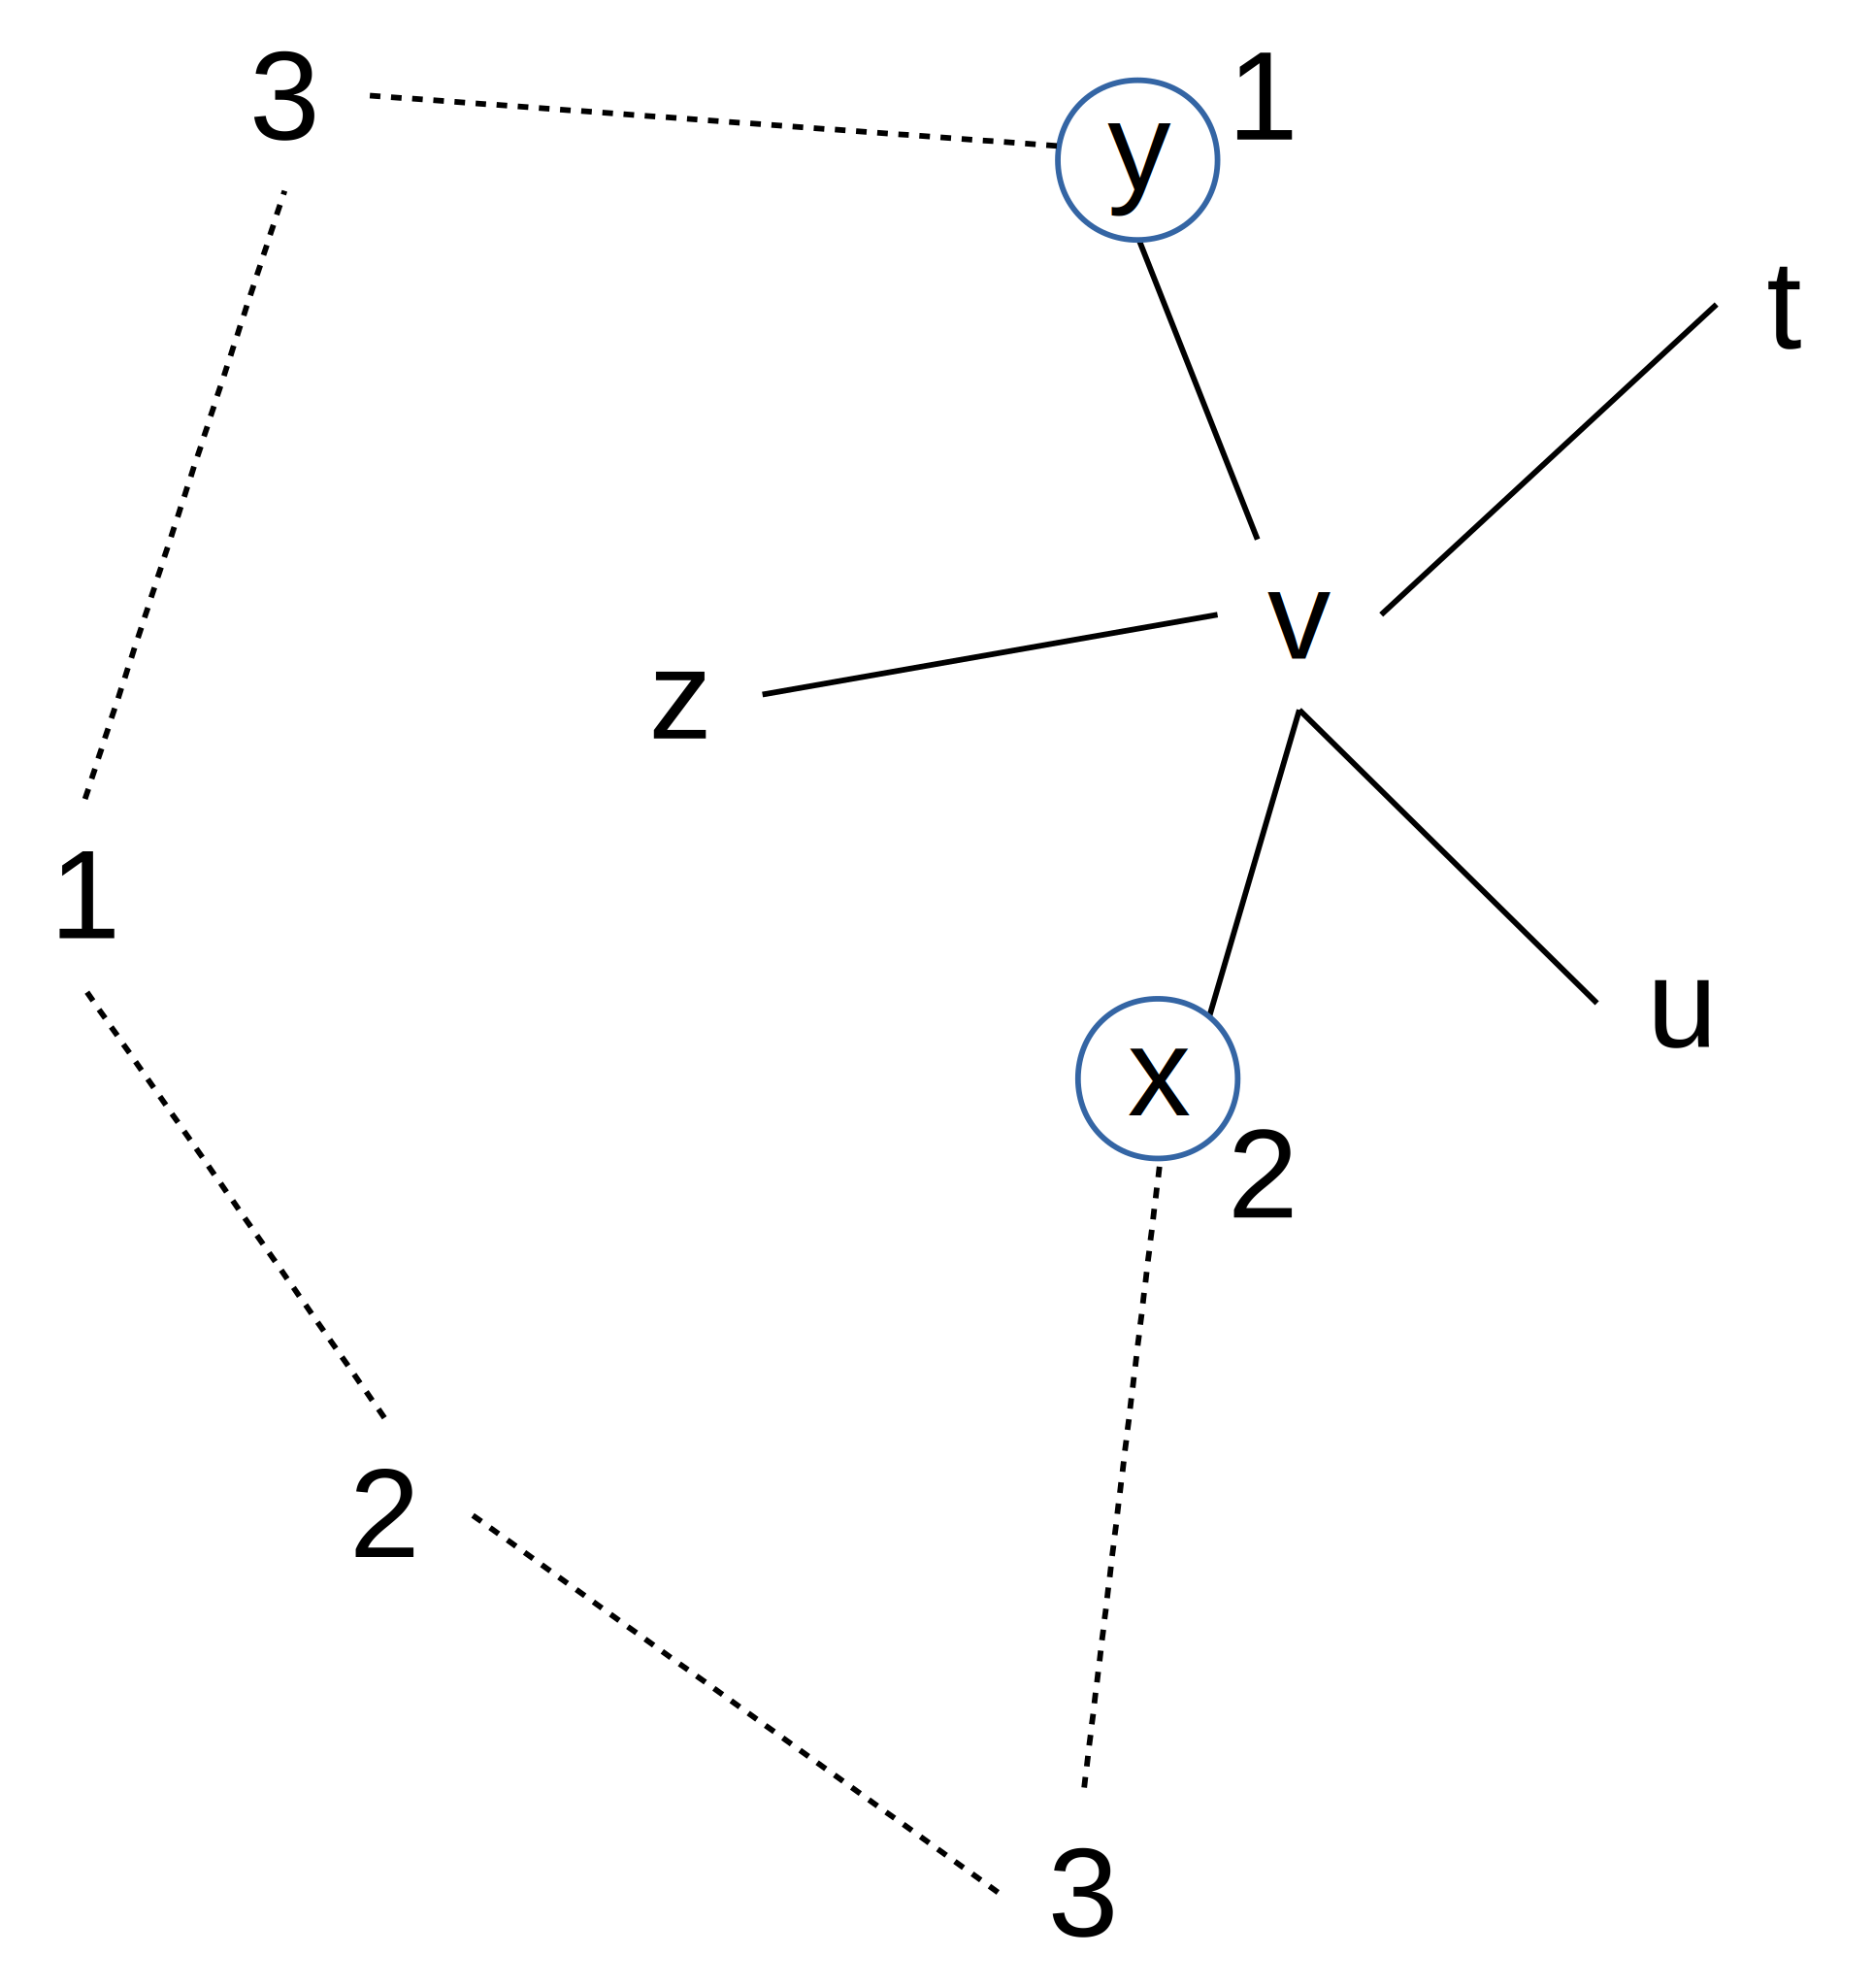
\includegraphics[scale=0.5]{lectures/161125/pix/2.pdf}
                        \begin{itemize}
                            \item betrachte 5-Färbung $\mathcal{C} \colon V(G \setminus \{v\}) \mapsto \{1, \dots, 5\}$, die es nach Rekursion gibt
                            \item betrache $x,y \in V_{xy}$ und sei $V_{xy} \subset V(G)$ die Menge der Knoten mit $\mathcal{C}(x)$- oder $\mathcal{C}(y)$-Färbung
                                \begin{enumerate}
                                    \item es gibt \underline{keinen} Weg von $x \rightsquigarrow y$, der nur Knoten aus $V_{xy}$ nutzt
                                        \begin{itemize}
                                            \item Seien $V'_{xy}$ die $s \in V(G \setminus \{v\})$, die von $x$ nur via $V_{xy}$ erreicht werden
                                            \item Färbe um:
                                            \begin{math}
                                                \mathcal{C'}(s) =
                                                    \begin{cases}
                                                        \mathcal{C}(s) & s \not \in V'_{xy}\\
                                                        \mathcal{C}(y) & s \in V'_{xy}, ~ \mathcal{C}(s) = \mathcal{C}(x)\\
                                                        \mathcal{C}(x) & s \in V'_{xy}, ~ \mathcal{C}(s) = \mathcal{C}(y)
                                                    \end{cases}
                                            \end{math}\\\\
                                            ``Tausche Farben auf $V'_{xy}$'' $\Rightarrow \mathcal{C'}(x) = \mathcal{C'}(y) = \mathcal{C}(y)$
                                        \end{itemize}
                                    \item es gibt einen solchen Pfad $x \rightsquigarrow y$ mit allen Knoten in $V_{xy}$
                                    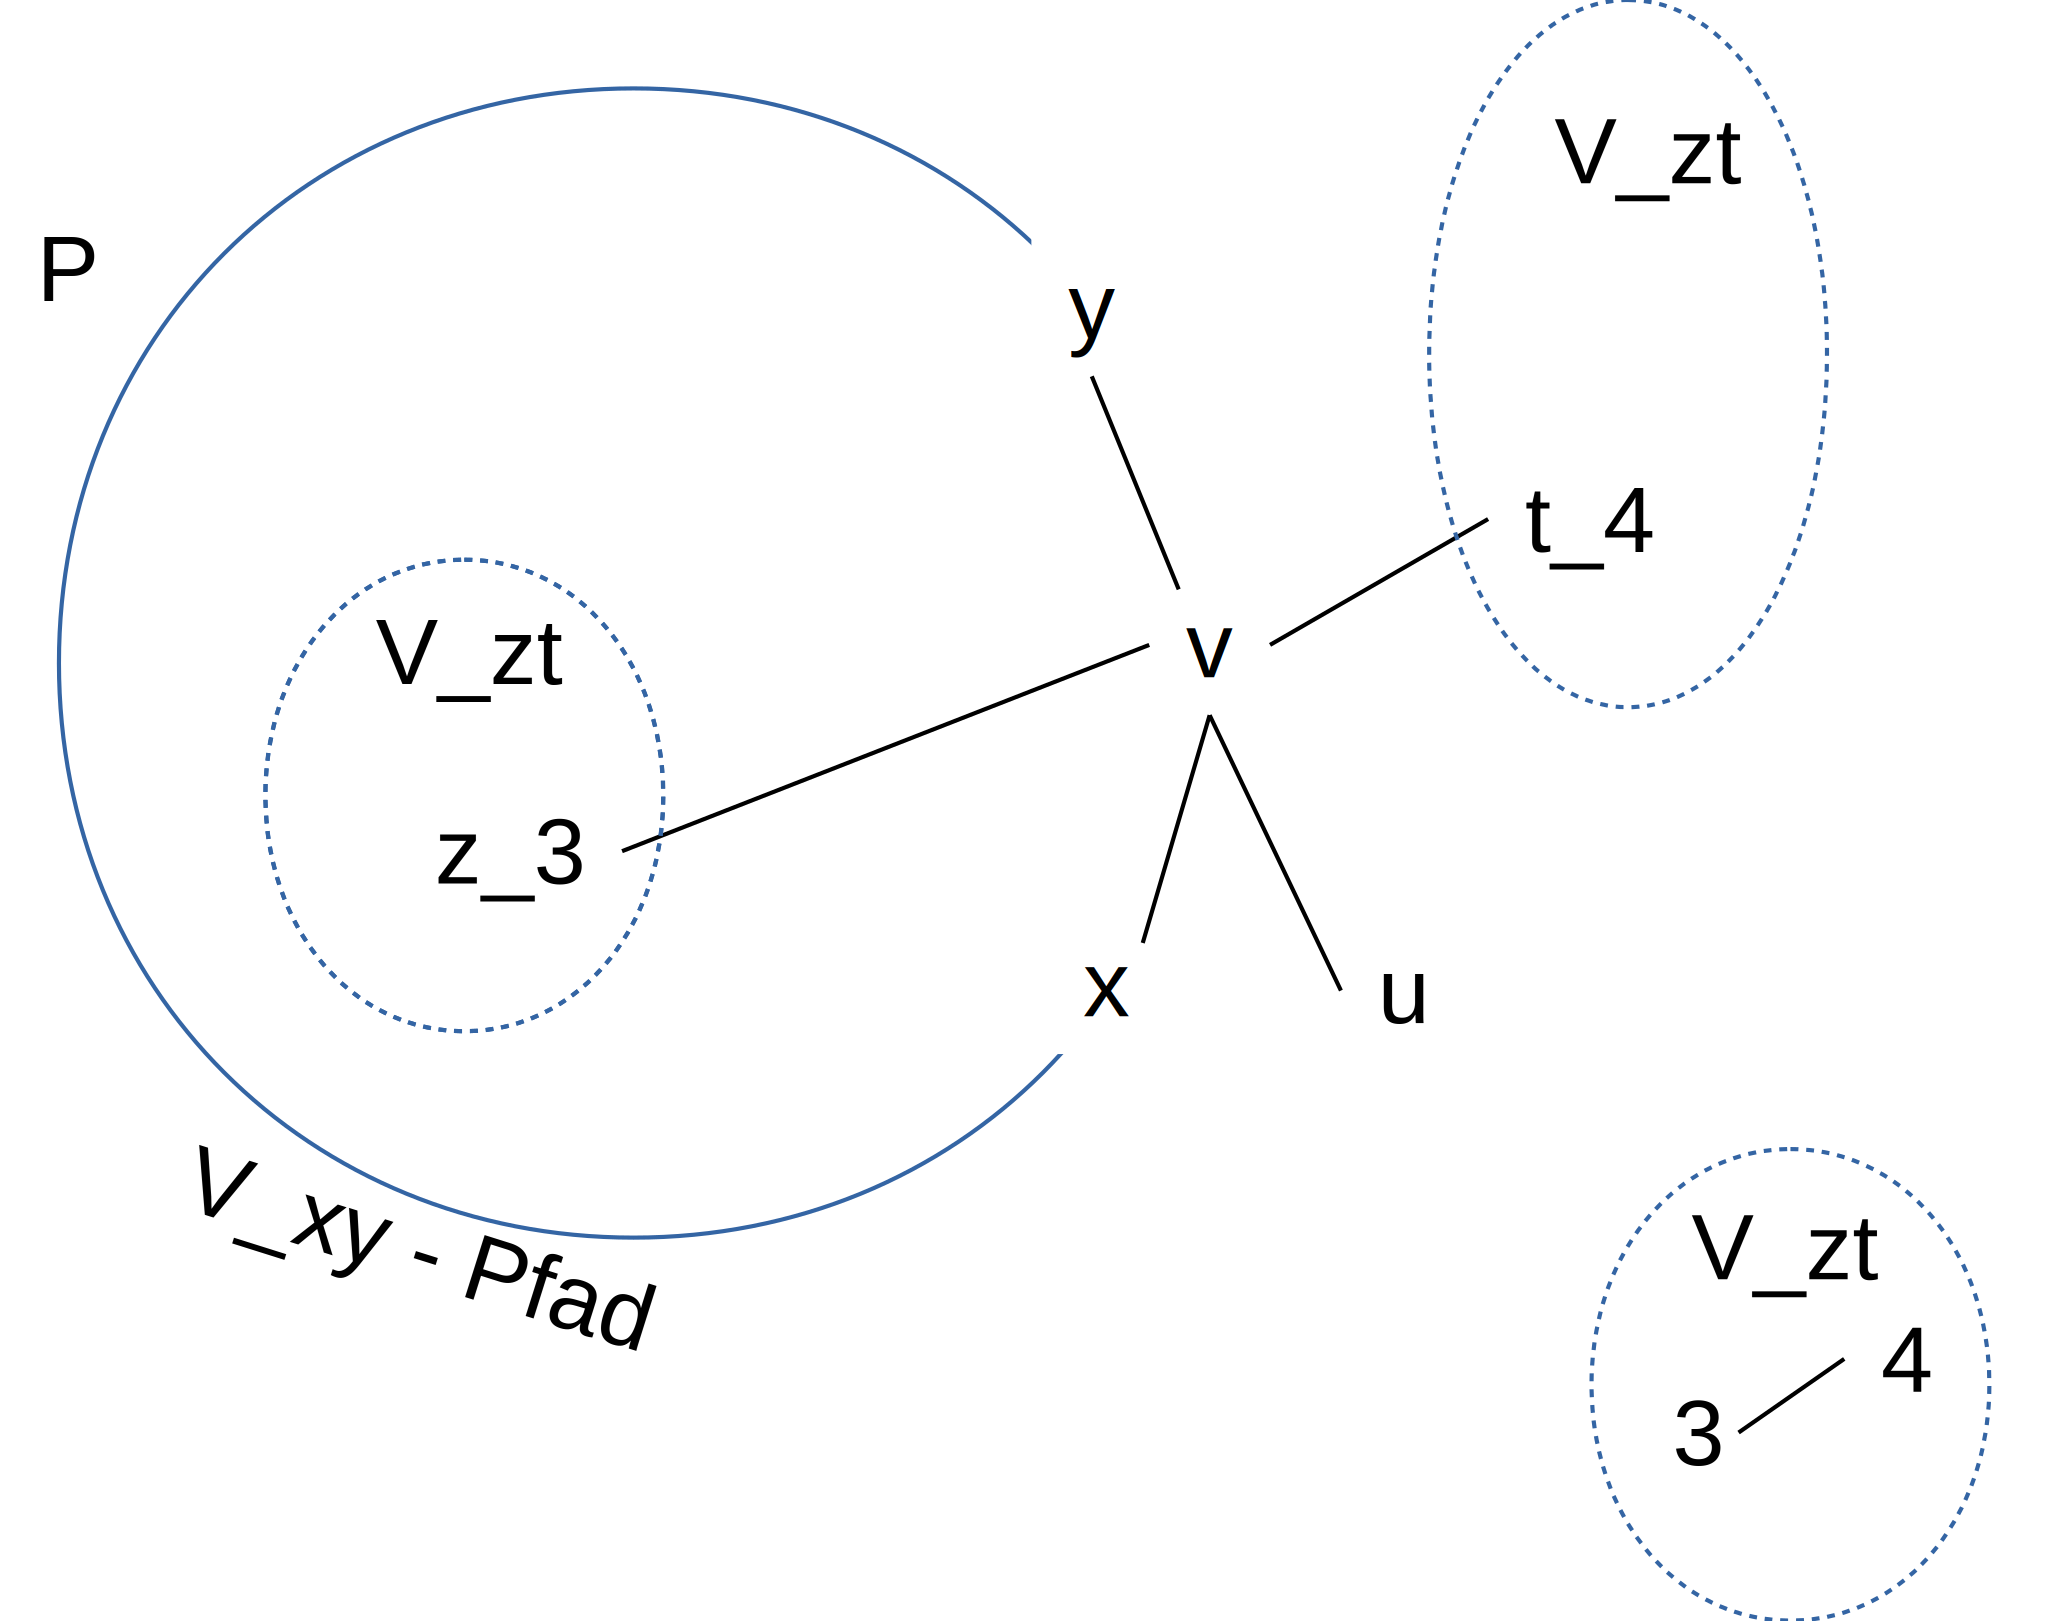
\includegraphics[scale=0.5]{lectures/161125/pix/3.pdf}
                                        \begin{itemize}
                                            \item $V_{zt}$: alle Knoten in $V(G \setminus \{v\})$, die $\mathcal{C}(t)$ oder $\mathcal{C}(z)$ gefärbt sind
                                            \item $V_{xy} \cap V_{zt} = \emptyset$!
                                            \item $V'_{zt}$ kann nur via eines $s \in P$ einen Knoten in $V_{zt} \setminus V'_{zt}$ erreichen
                                        \end{itemize}
                                        Damit lassen sich $z,t$ analog zu Fall (a) färben.
                                \end{enumerate}
                        \end{itemize}
                \end{enumerate}
        \end{description}
    \item[Theorem] Jeder planare Graph ist 4-färbbar
        \begin{description}
            \item[Proof] Es gibt eine Menge von 1936 4-färbbaren Karten, jede nicht Teil eines kleinsten Gegenbeispiels... (Appel, Haken, 1976).
            $\Rightarrow$ Es folgt, dass es kein kleinstes Gegenbeispiel gibt.
        \end{description}
\end{description}

\subsection{Zufallsgraphen}
Sei $G=(V,E)$ mit $V=\{1, \dots, n\}$ fixiert. Wir wollen nun Kanten zufällig auswählen auf dieser fixierten Kantenmenge $\{1, \dots, n\}$, um zufällige Graphen zu generieren. 
Die Menge dieser Zufallsgraphen nennen wir $\mathcal{G}$. \underline{Jede} Kante wird mit Wahrscheinlichkeit $p \in [0, \dots, 1]$ gewählt. 
Sei $G_0$ ein bestimmter Graph. Das Ereignis $\{G_0\}$ mit $G_0$ und m Kanten hat die Wahrscheinlichkeit $p^m \cdot (1-p)^{{n \over 2}-m}$. 
Wahrscheinlichkeitsmaß auf 
$\mathcal{G} ~ \forall e \in [v]^2$\\
$\Omega_e=\{0_e, 1_e\}$\\
$\mathbb{P}(\{1_e\})=p$\\
$\mathbb{P}(\{0_e\})=1-p$\\
$\Omega_\mathcal{G} = \prod\limits_{e \in [v]^2} \Omega_e$

\begin{description}
    \item[Beispiele] Fixiere Graph $H$, $V(H) = V(G)$, ist $H \leqslant G$? \\
        Mit $p^l$, $|E(H)| = l$, $|V(H)| = k$, aber falls $H$ induzierter Teilgraph von $G$ sein soll? \\
         - Nur $p^l (1-p)^{\binom{k}{2} - l}$. \\
        Und was ist mit Subgraph-Isomorphismus?
        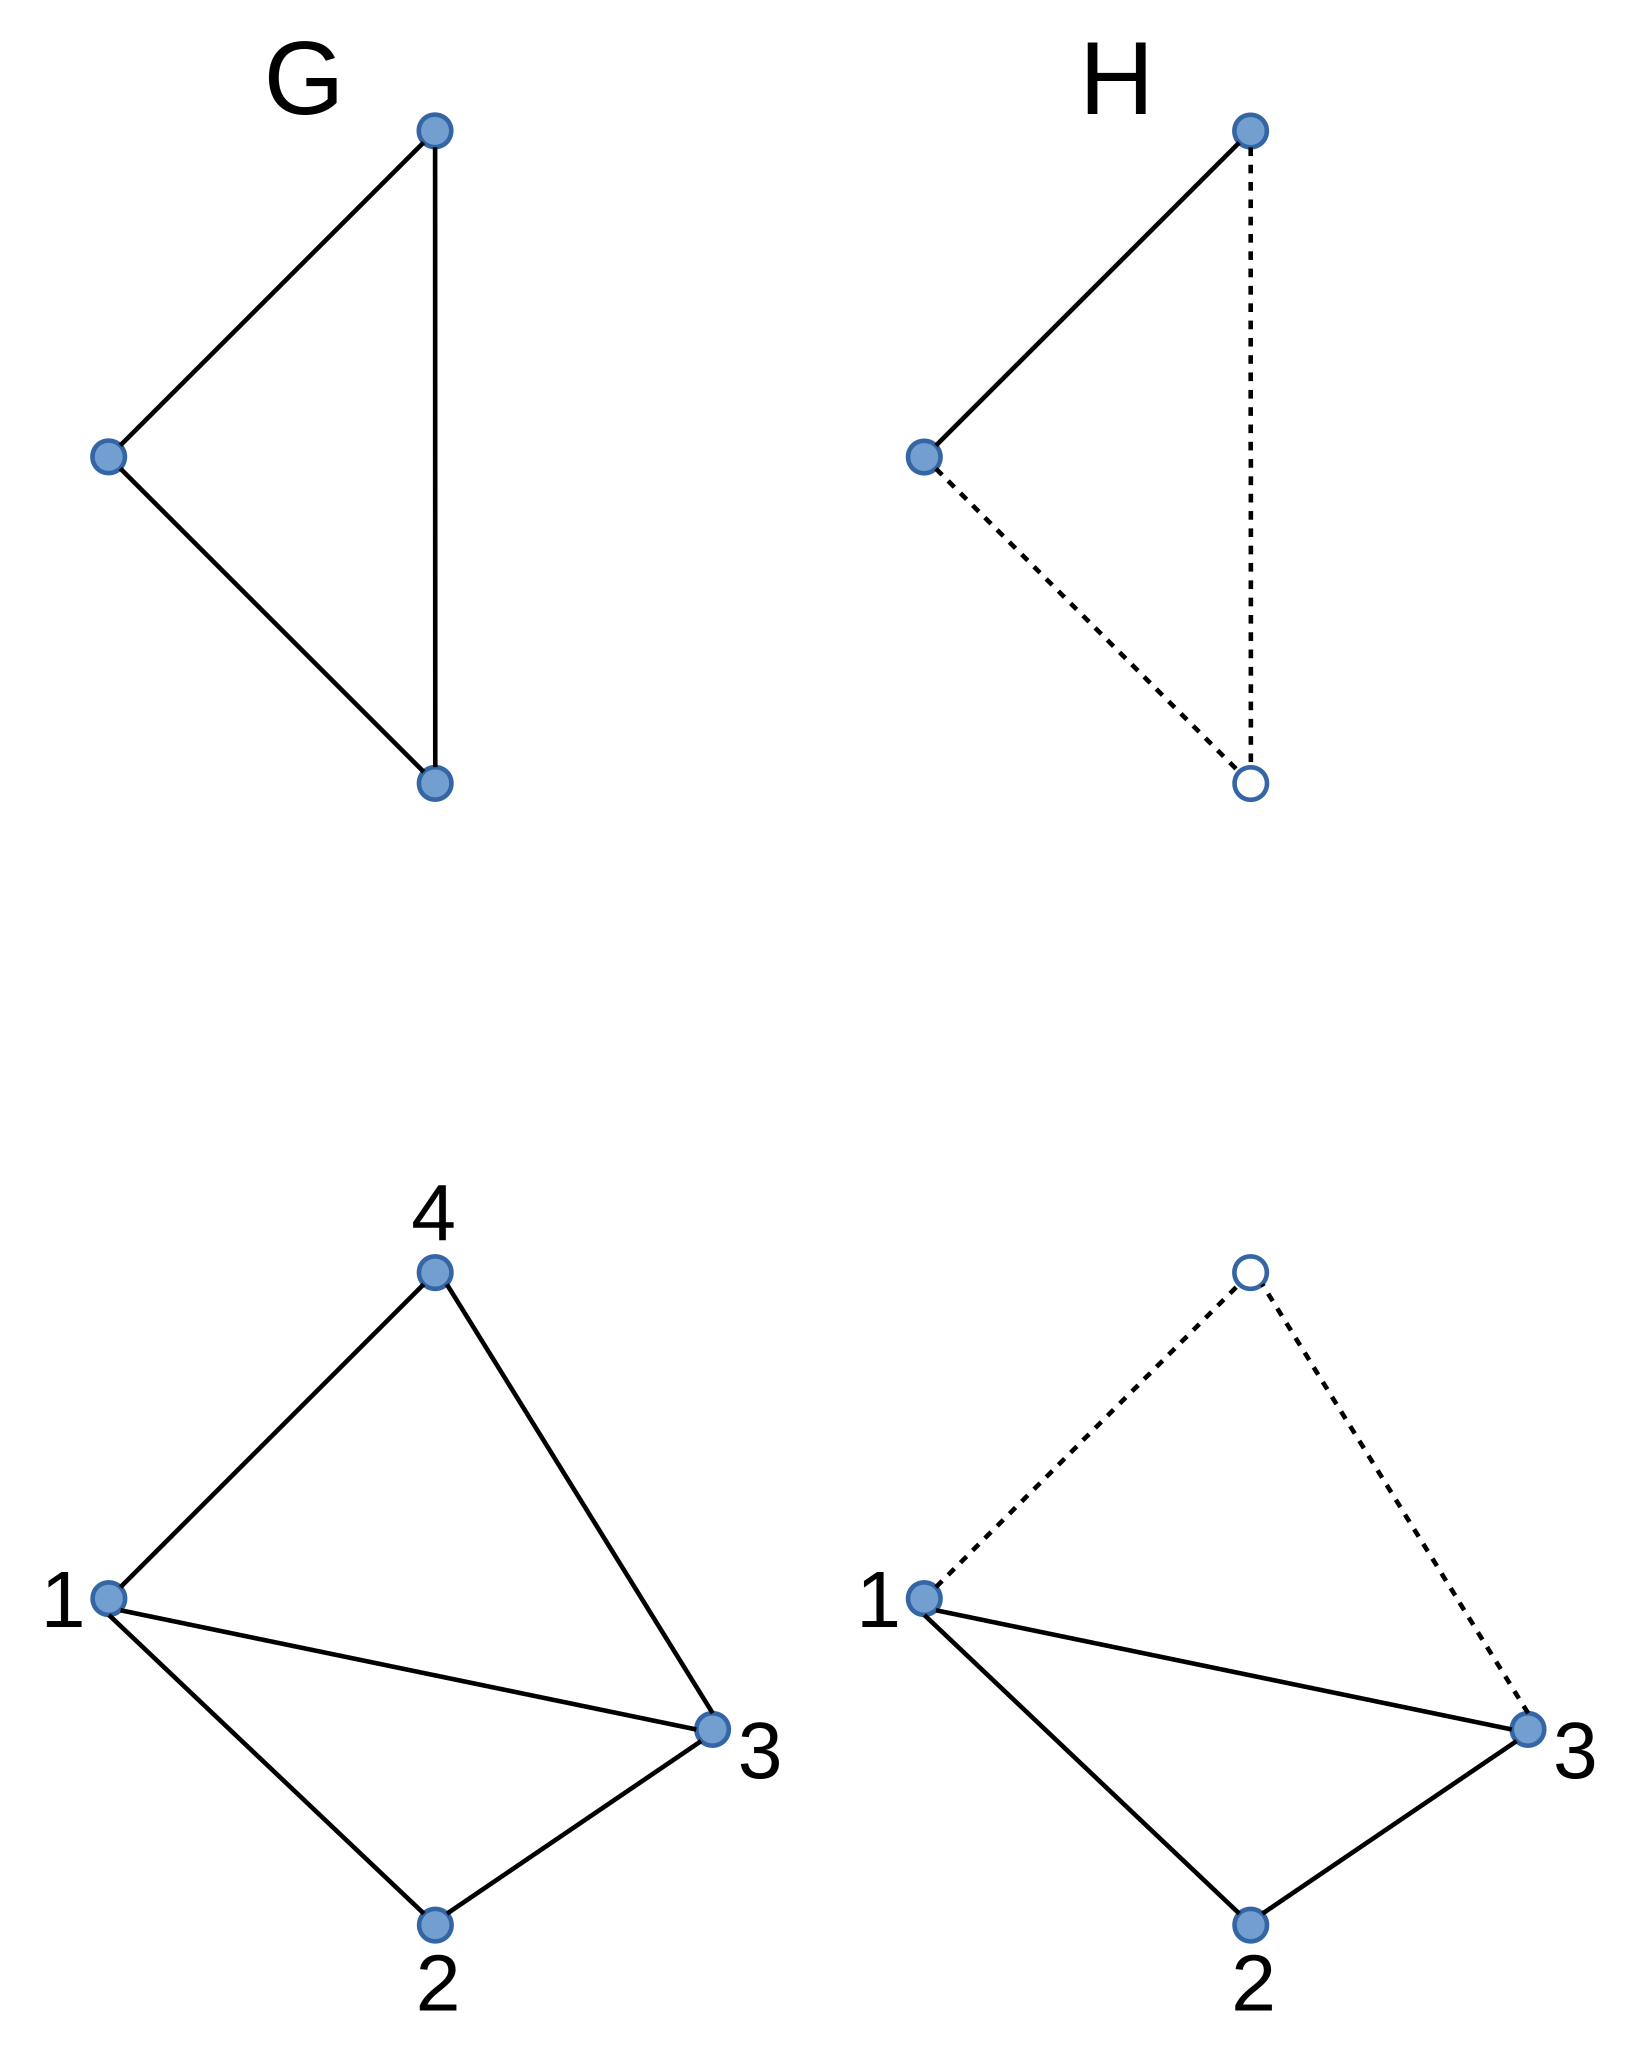
\includegraphics[scale=0.5]{lectures/161125/pix/4.pdf}
        \begin{itemize}
            \item Ereignismengen überlappen
            \item kompliziert
        \end{itemize}
\end{description}

\subsection{Eigenschaften fast aller Graphen}
Falls die Wahrscheinlichkeit, dass $P(G \in \mathcal{G}) \rightarrow 1$ für $n \rightarrow \infty$, dann geschieht $G$ fast sicher.
\begin{description}
    \item[Pro:] Gegeben jedes $H$ als Isomorphie-Klasse, $n \rightarrow \infty$ und $p \in ]0,1[ = (0,1)$, induzierte Kopie von $H$. 
    Dann haben fast alle $G$ in $\mathcal{G}(n,p)$ haben mindestens eine induzierte Kopie von $H$.
    \item[Prf:] Sei $H$ gegeben, $K=V(H)$. Sei $K \leqslant n$. $H$ ist (subgraph-) isomorph zu $G$ mit Wahrscheinlichkeit $r < 0$ ($G$ ist zufällig!). 
        Teile $G$ in $\lfloor {n \over k} \rfloor$ Teilgraphen, um genau so viele ``Versuche'' (für $r > 0$) zu haben. 
        $P(H \not \subseteq G$ induziert) $\leqslant (1-r)^{\lfloor {n \over k} \rfloor} \xrightarrow{n \rightarrow \infty} 0$
\end{description}


\newpage

\section{Vorlesung 25.11.2016}
\subsection{Färbung von Graphen}
\subsubsection{Vertexfärbung}
Zwei durch eine Kante verbundene Knoten haben unterschiedliche Farben.\\
Beispiel wäre eine Landkarte auf der mit so wenig wie möglich Farben die Länder ausgemalt werden, ohne zwei benachbarte Länder gleichfarbig zu haben. Hierbei entspricht jede Facette einen Knoten.\\
\includegraphics[width=0.4\textwidth]{lectures/161125/pix/Vertexfaerbung}
\begin{description}
    \item[Vertexfärbung] Eine Vertexfärbung eines Graphen $G=(V,E)$ ist eine Abbildung $\mathcal{C} \colon V \mapsto \mathcal{S}$, mit $\mathcal{S}=$ Menge der Farben. Es gilt, dass $\mathcal{C}(v) \neq \mathcal{C}(w)$, mit $w,v \in \mathcal{S}$, wenn $v$ und $w$ adjazent ($\{v,w\} \in E$) sind. Die Elemente von $\mathcal{S}$ heißen \emph{Farben}.
    \item[k-Färbung] Ein Graph $G$ ist $k$-färbbar, wenn es für eine Abbildung $\mathcal{C}$ eine Menge $\mathcal{S}=\{1,\dots,k\}$ gibt.
    \item[Chromatische Zahl] Eine chromatische Zahl $\chi(G)$ ist die kleinste natürliche Zahl $k$, sodass G $k$-färbbar ist. $\chi(G) \leqslant \Delta(G) + 1$, mit $\Delta(G) = $ maximaler Grad von $G$
        \begin{description}
            \item[Proof (greedy)] Färbe $v_i$ der Vertices $v_1 \dots v_n$ mit der kleinsten Farbe, die nicht von einem Nachbarn von $v_i$ benutzt wird. Da wir max. $\Delta(G)$ viele Nachbarn für $v_i$ haben, gibt es immer eine freie Farbe.
        \end{description}
        $\chi(G) \geqslant$ Größe der größten Clique
    \item[Lemma] Für jeden einfachen planaren Graphen $G$ ist der Durchschnittsgrad $d(G) < 6$
        \begin{description}
            \item[Proof] $d(G) = 2 \cdot {|E| \over |V|}$ mit $|V| \leqslant 3$, $|E| \leqslant 3  \cdot |V| - 6$, dann $d(G) \leqslant {2(3 \cdot |V|-6) \over |V|} = 6-{12 \over |V|}$
        \end{description}
    \item[Theorem] Jeder simple planare Graph $G$ hat $\chi(G) \leqslant 6$
        \begin{description}
            \item[Proof] Annahme: Jeder simple planare Graph mit $|V| = n$ ist $6$-färbbar.
            \begin{itemize}
                \item Sei $G$ hiermit ein simpler planarer Graph mit $|V| = n+1$
                \item Vom Lemma wissen wir, dass $w \in V$ mit $d(w) \leqslant 5$ existiert
                \item Sei $G' = G \setminus \{w\}$. Via Induktionshypothese ist $G'$ 6-färbbar. Das tun wir dann.
                \item Färbe $w$ mit der (min.) freien Farbe, um $G$ zu färben
            \end{itemize}
        \end{description}
    \item[Theorem] Für jeden simplen planaren Graphen $G$ gilt, dass $\chi(G) \leqslant 5$
        \begin{description}
            \item[Proof] Sei $G=(V,E)$ planar
                \begin{enumerate}
                    \item Falls $|V| \leqslant 5 \rightarrow$ trivial
                    \item Für alle $v \in V(G)$ mit $deg(v) < 5$, färbe $v$ und arbeite mit $G \setminus \{v\}$
                    \item $G$ hat Vertex $v$ mit $deg(v) = 5$
                        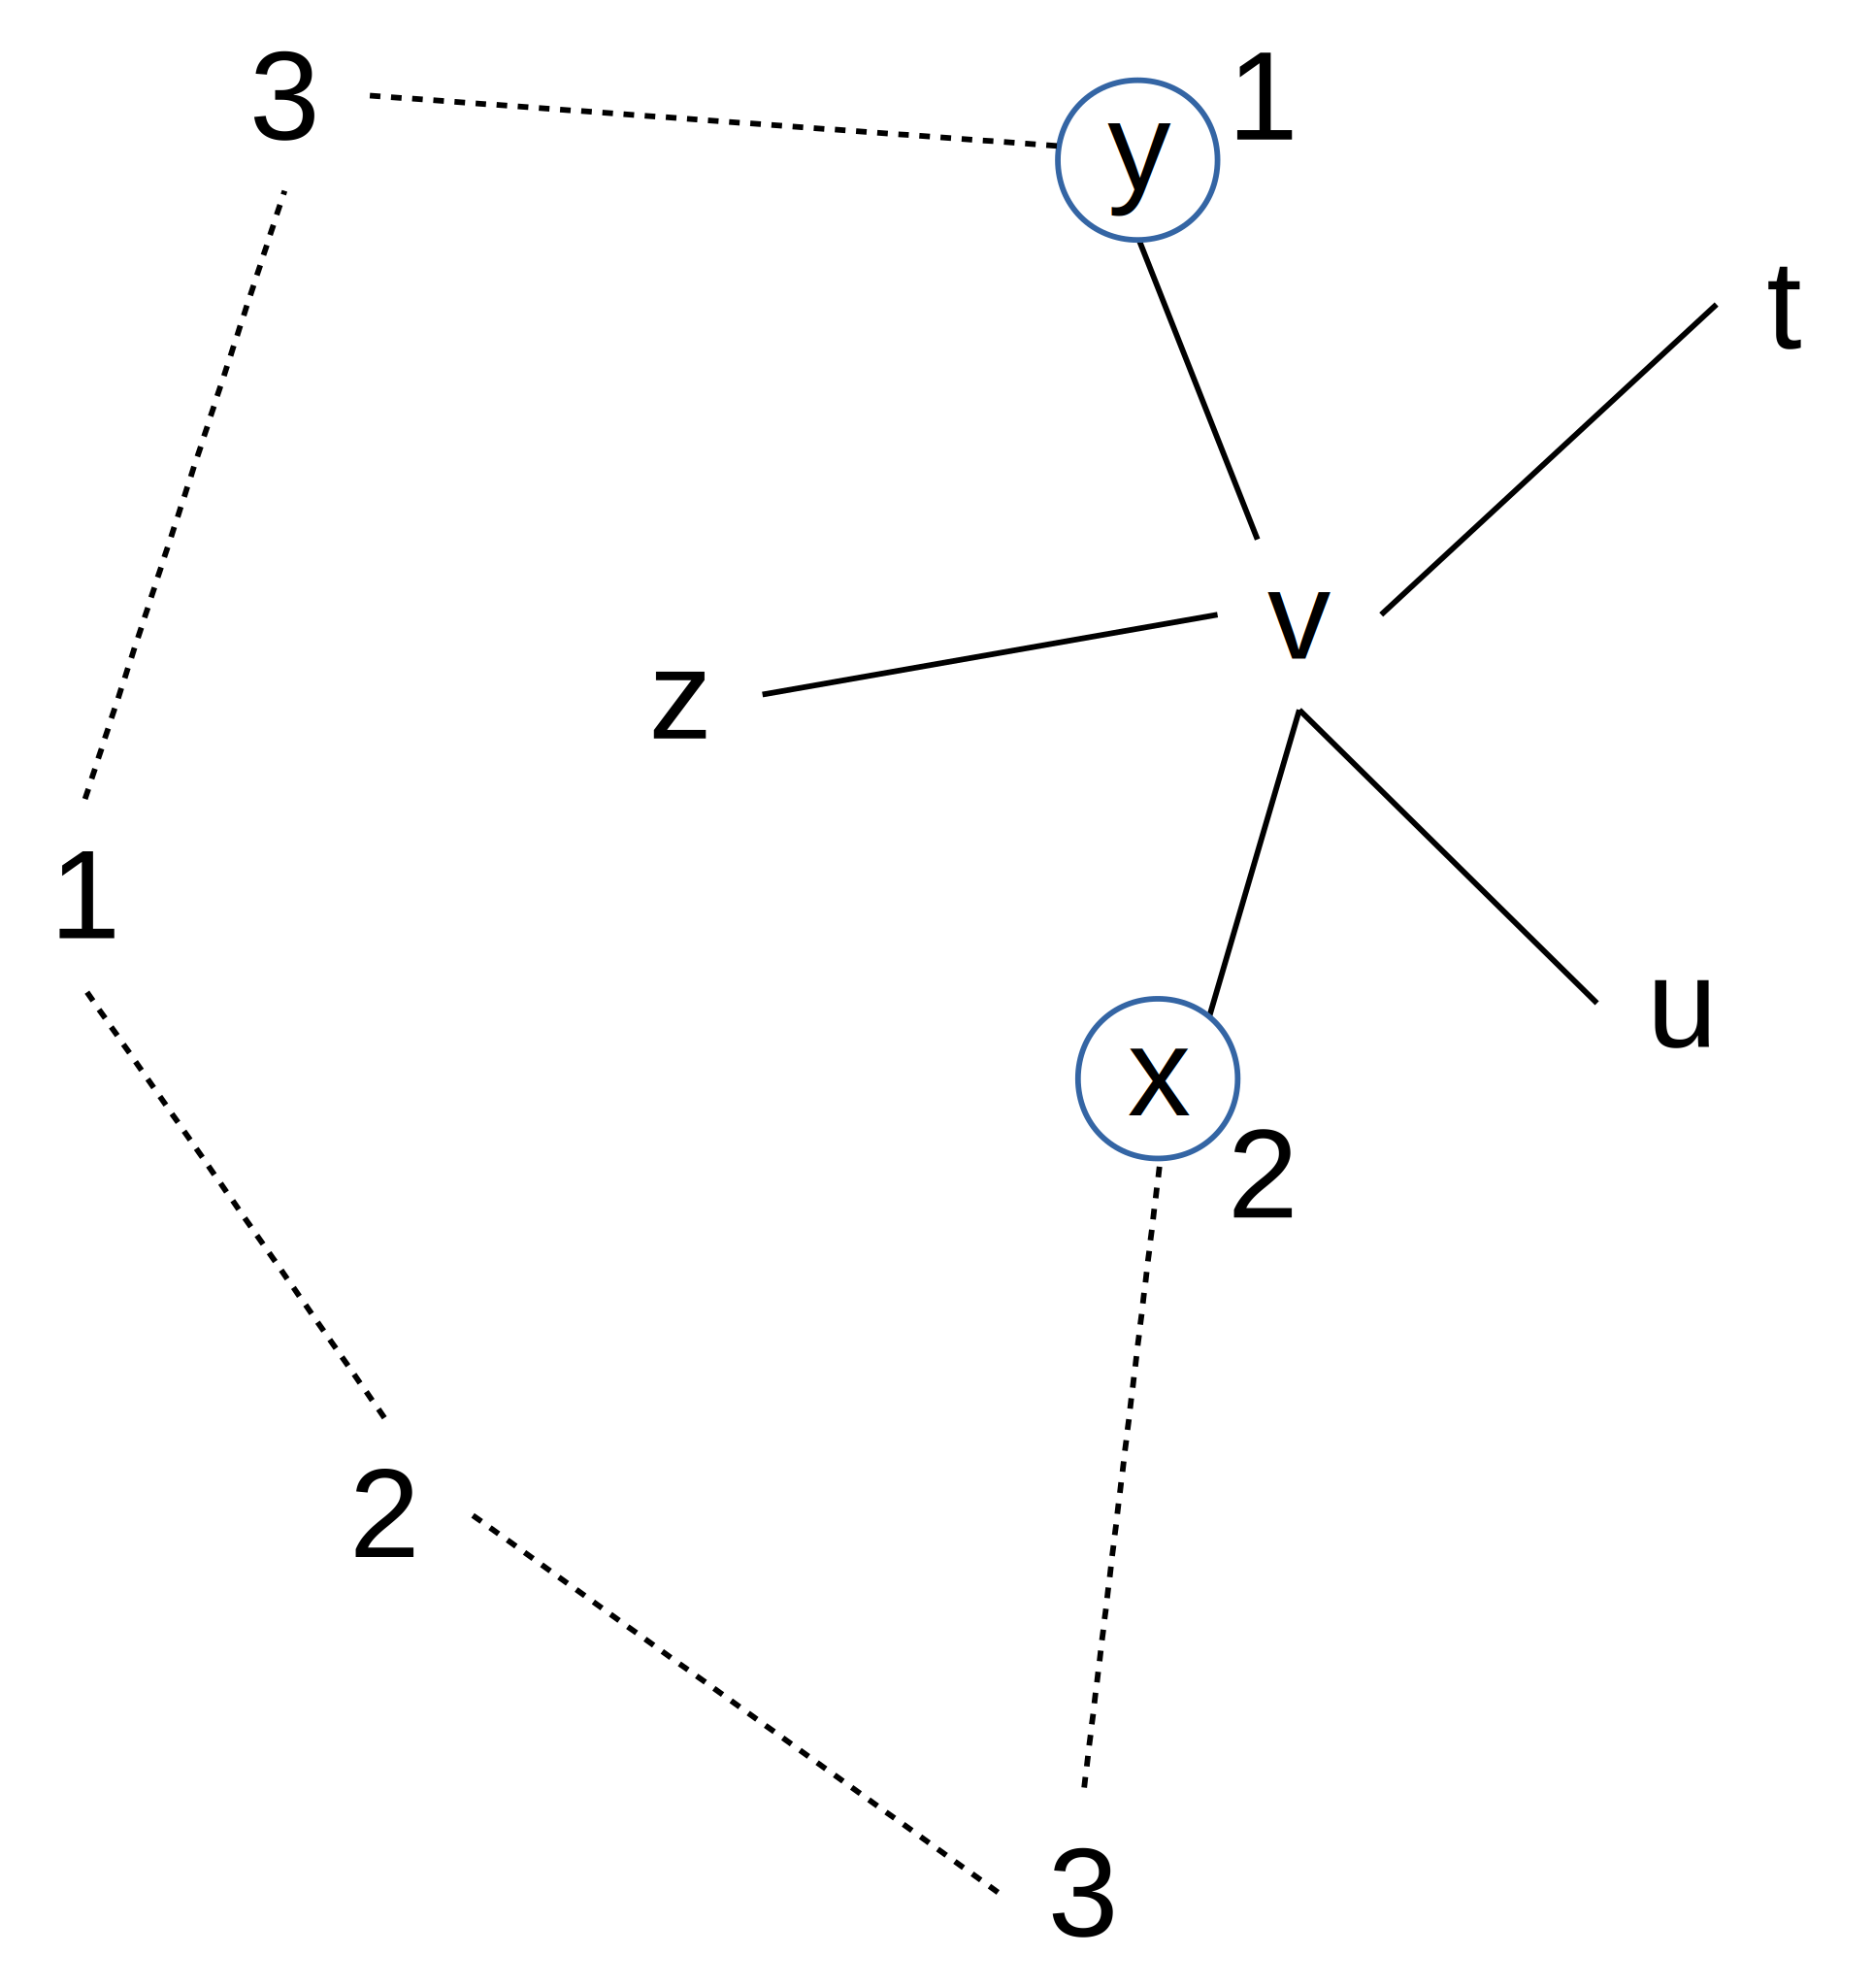
\includegraphics[scale=0.5]{lectures/161125/pix/2.pdf}
                        \begin{itemize}
                            \item betrachte 5-Färbung $\mathcal{C} \colon V(G \setminus \{v\}) \mapsto \{1, \dots, 5\}$, die es nach Rekursion gibt
                            \item betrache $x,y \in V_{xy}$ und sei $V_{xy} \subset V(G)$ die Menge der Knoten mit $\mathcal{C}(x)$- oder $\mathcal{C}(y)$-Färbung
                                \begin{enumerate}
                                    \item es gibt \underline{keinen} Weg von $x \rightsquigarrow y$, der nur Knoten aus $V_{xy}$ nutzt
                                        \begin{itemize}
                                            \item Seien $V'_{xy}$ die $s \in V(G \setminus \{v\})$, die von $x$ nur via $V_{xy}$ erreicht werden
                                            \item Färbe um:
                                            \begin{math}
                                                \mathcal{C'}(s) =
                                                    \begin{cases}
                                                        \mathcal{C}(s) & s \not \in V'_{xy}\\
                                                        \mathcal{C}(y) & s \in V'_{xy}, ~ \mathcal{C}(s) = \mathcal{C}(x)\\
                                                        \mathcal{C}(x) & s \in V'_{xy}, ~ \mathcal{C}(s) = \mathcal{C}(y)
                                                    \end{cases}
                                            \end{math}\\\\
                                            ``Tausche Farben auf $V'_{xy}$'' $\Rightarrow \mathcal{C'}(x) = \mathcal{C'}(y) = \mathcal{C}(y)$
                                        \end{itemize}
                                    \item es gibt einen solchen Pfad $x \rightsquigarrow y$ mit allen Knoten in $V_{xy}$
                                    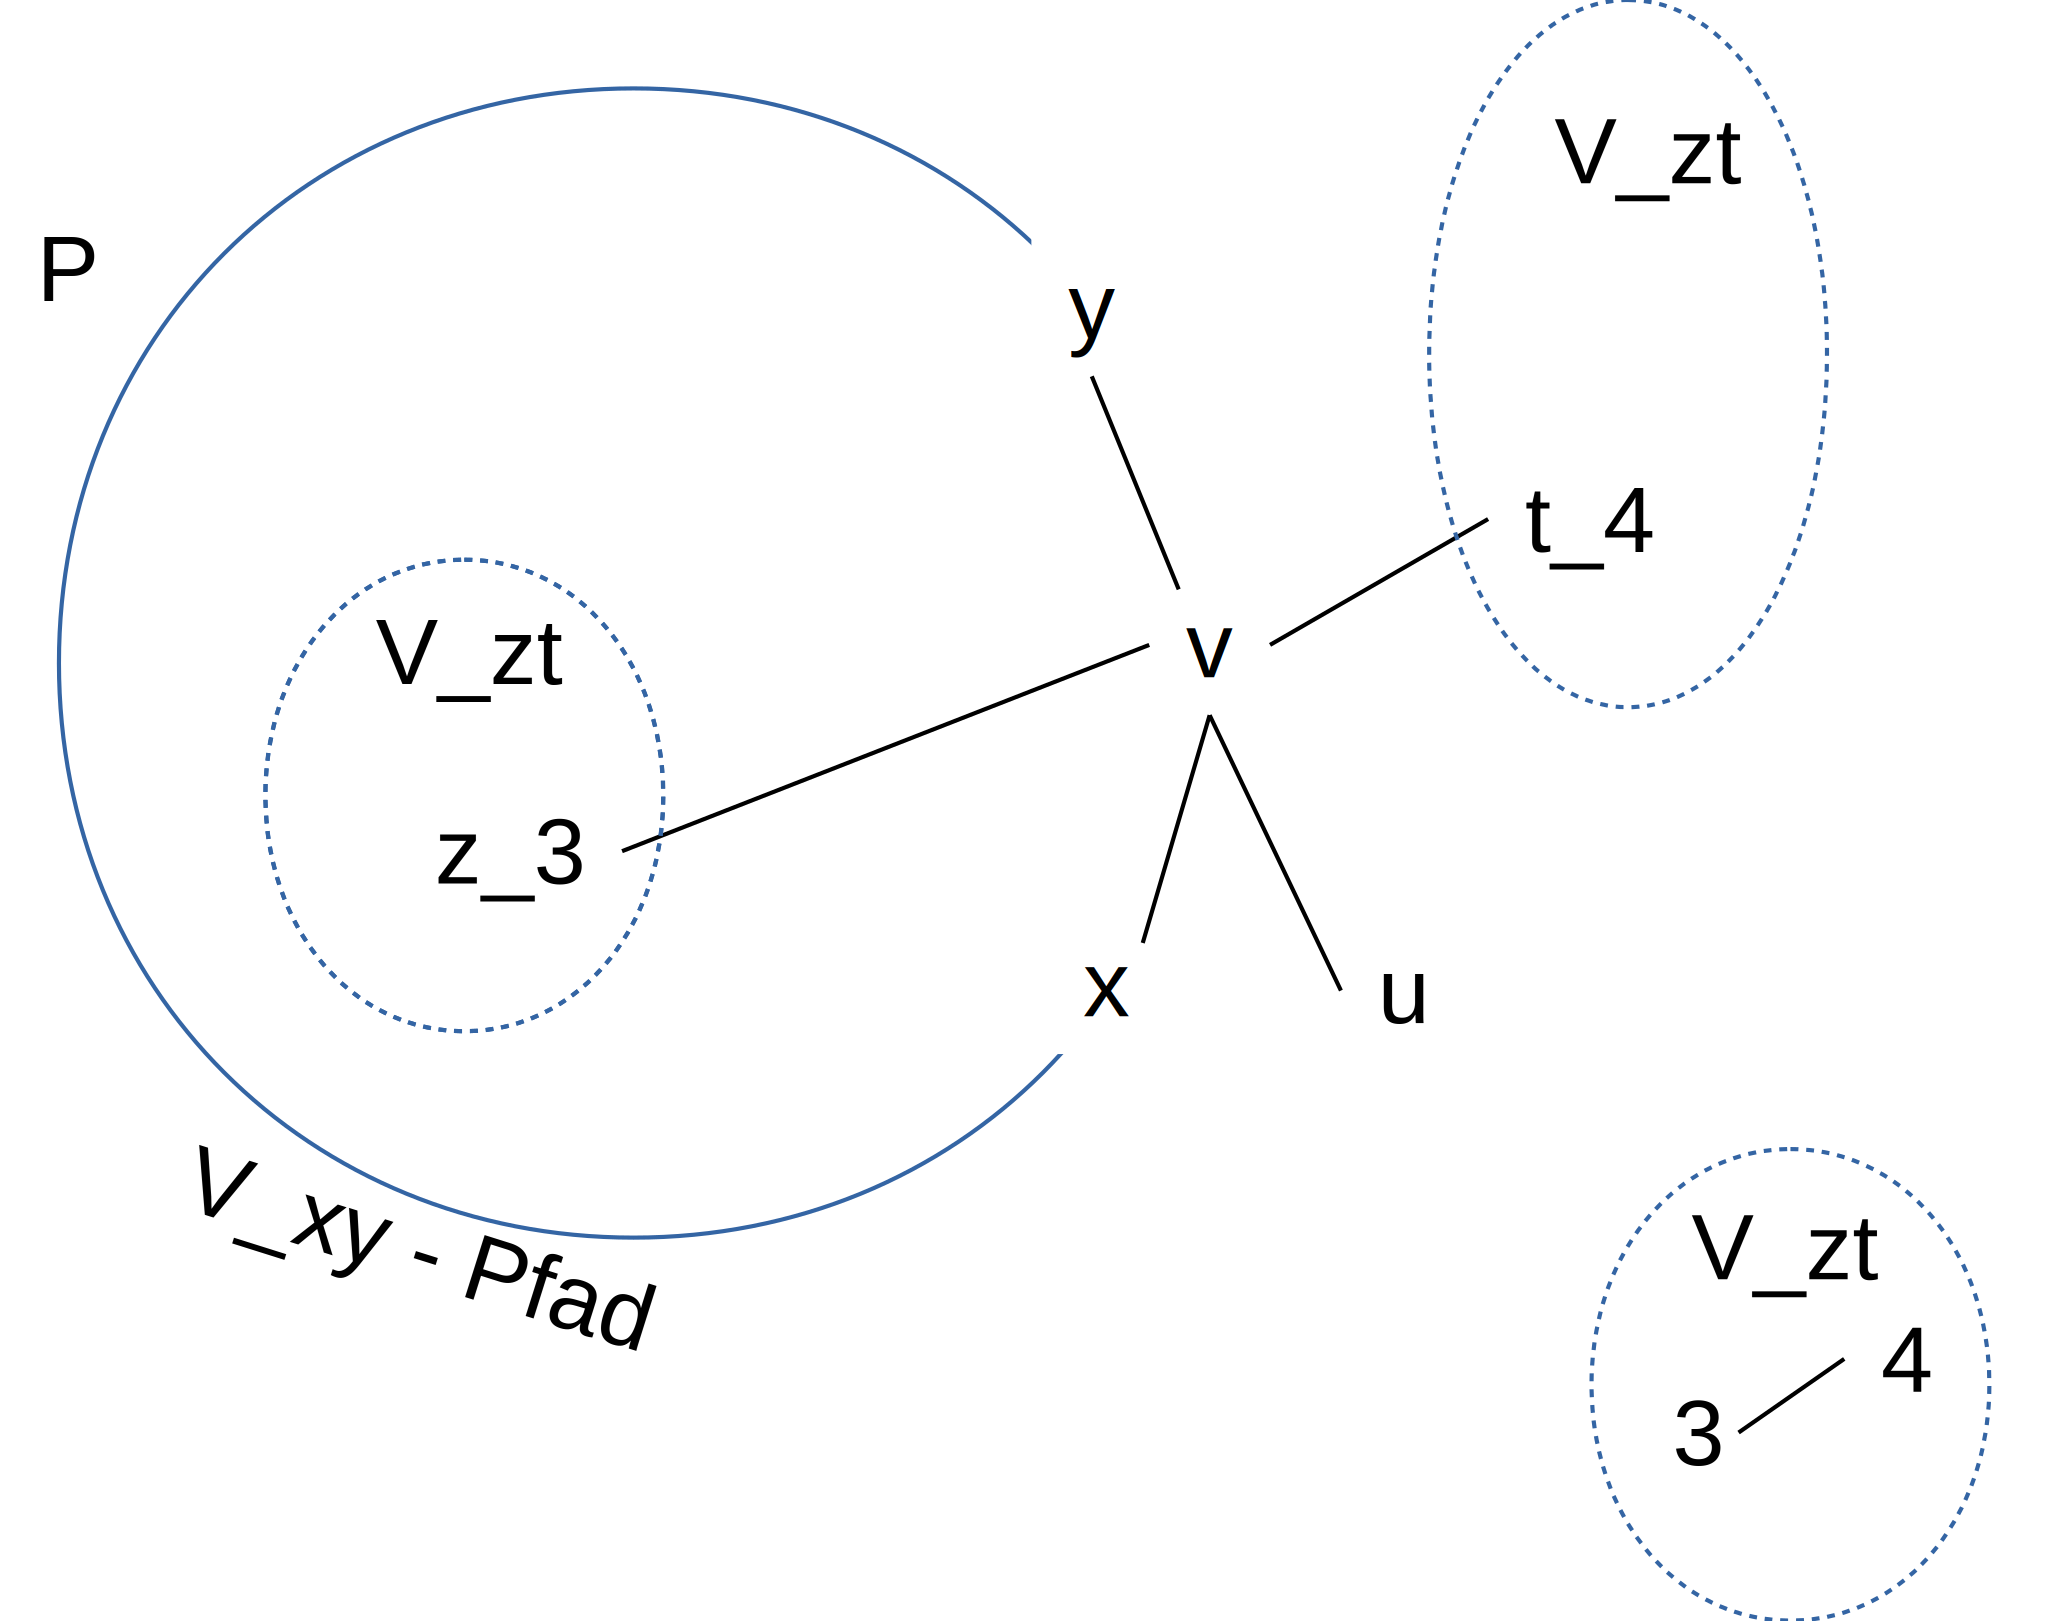
\includegraphics[scale=0.5]{lectures/161125/pix/3.pdf}
                                        \begin{itemize}
                                            \item $V_{zt}$: alle Knoten in $V(G \setminus \{v\})$, die $\mathcal{C}(t)$ oder $\mathcal{C}(z)$ gefärbt sind
                                            \item $V_{xy} \cap V_{zt} = \emptyset$!
                                            \item $V'_{zt}$ kann nur via eines $s \in P$ einen Knoten in $V_{zt} \setminus V'_{zt}$ erreichen
                                        \end{itemize}
                                        Damit lassen sich $z,t$ analog zu Fall (a) färben.
                                \end{enumerate}
                        \end{itemize}
                \end{enumerate}
        \end{description}
    \item[Theorem] Jeder planare Graph ist 4-färbbar
        \begin{description}
            \item[Proof] Es gibt eine Menge von 1936 4-färbbaren Karten, jede nicht Teil eines kleinsten Gegenbeispiels... (Appel, Haken, 1976).
            $\Rightarrow$ Es folgt, dass es kein kleinstes Gegenbeispiel gibt.
        \end{description}
\end{description}

\subsection{Zufallsgraphen}
Sei $G=(V,E)$ mit $V=\{1, \dots, n\}$ fixiert. Wir wollen nun Kanten zufällig auswählen auf dieser fixierten Kantenmenge $\{1, \dots, n\}$, um zufällige Graphen zu generieren. 
Die Menge dieser Zufallsgraphen nennen wir $\mathcal{G}$. \underline{Jede} Kante wird mit Wahrscheinlichkeit $p \in [0, \dots, 1]$ gewählt. 
Sei $G_0$ ein bestimmter Graph. Das Ereignis $\{G_0\}$ mit $G_0$ und m Kanten hat die Wahrscheinlichkeit $p^m \cdot (1-p)^{{n \over 2}-m}$. 
Wahrscheinlichkeitsmaß auf 
$\mathcal{G} ~ \forall e \in [v]^2$\\
$\Omega_e=\{0_e, 1_e\}$\\
$\mathbb{P}(\{1_e\})=p$\\
$\mathbb{P}(\{0_e\})=1-p$\\
$\Omega_\mathcal{G} = \prod\limits_{e \in [v]^2} \Omega_e$

\begin{description}
    \item[Beispiele] Fixiere Graph $H$, $V(H) = V(G)$, ist $H \leqslant G$? \\
        Mit $p^l$, $|E(H)| = l$, $|V(H)| = k$, aber falls $H$ induzierter Teilgraph von $G$ sein soll? \\
         - Nur $p^l (1-p)^{\binom{k}{2} - l}$. \\
        Und was ist mit Subgraph-Isomorphismus?
        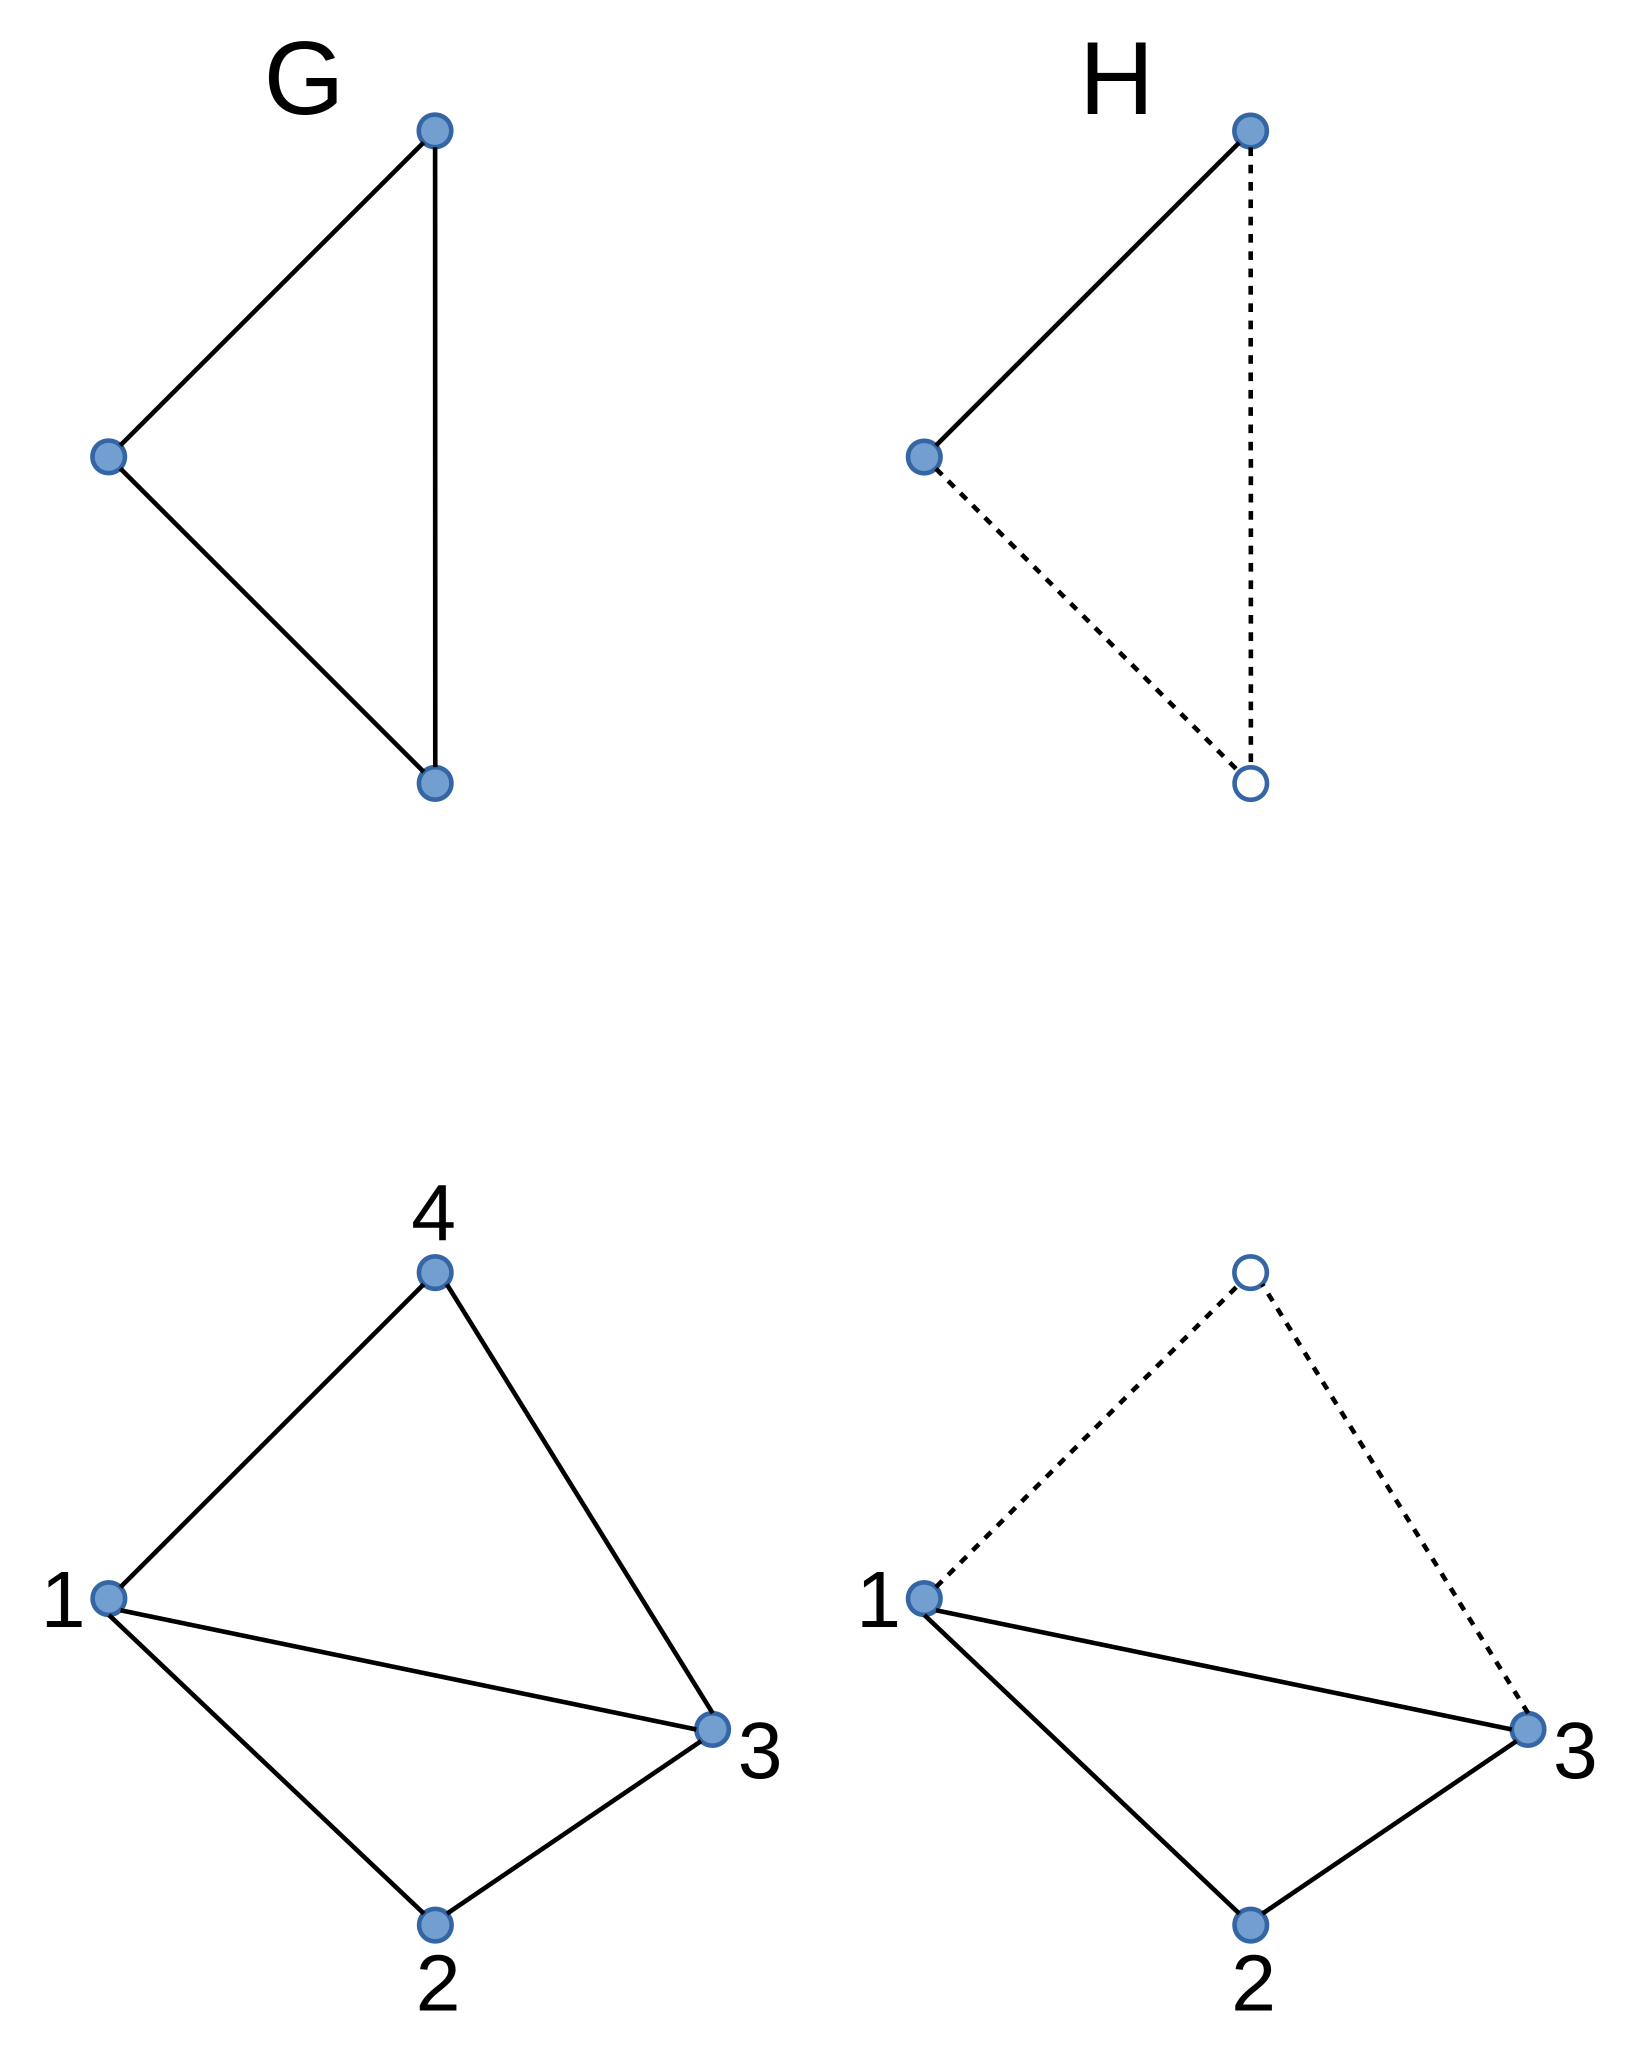
\includegraphics[scale=0.5]{lectures/161125/pix/4.pdf}
        \begin{itemize}
            \item Ereignismengen überlappen
            \item kompliziert
        \end{itemize}
\end{description}

\subsection{Eigenschaften fast aller Graphen}
Falls die Wahrscheinlichkeit, dass $P(G \in \mathcal{G}) \rightarrow 1$ für $n \rightarrow \infty$, dann geschieht $G$ fast sicher.
\begin{description}
    \item[Pro:] Gegeben jedes $H$ als Isomorphie-Klasse, $n \rightarrow \infty$ und $p \in ]0,1[ = (0,1)$, induzierte Kopie von $H$. 
    Dann haben fast alle $G$ in $\mathcal{G}(n,p)$ haben mindestens eine induzierte Kopie von $H$.
    \item[Prf:] Sei $H$ gegeben, $K=V(H)$. Sei $K \leqslant n$. $H$ ist (subgraph-) isomorph zu $G$ mit Wahrscheinlichkeit $r < 0$ ($G$ ist zufällig!). 
        Teile $G$ in $\lfloor {n \over k} \rfloor$ Teilgraphen, um genau so viele ``Versuche'' (für $r > 0$) zu haben. 
        $P(H \not \subseteq G$ induziert) $\leqslant (1-r)^{\lfloor {n \over k} \rfloor} \xrightarrow{n \rightarrow \infty} 0$
\end{description}


\newpage

\section{Vorlesung 25.11.2016}
\subsection{Färbung von Graphen}
\subsubsection{Vertexfärbung}
Zwei durch eine Kante verbundene Knoten haben unterschiedliche Farben.\\
Beispiel wäre eine Landkarte auf der mit so wenig wie möglich Farben die Länder ausgemalt werden, ohne zwei benachbarte Länder gleichfarbig zu haben. Hierbei entspricht jede Facette einen Knoten.\\
\includegraphics[width=0.4\textwidth]{lectures/161125/pix/Vertexfaerbung}
\begin{description}
    \item[Vertexfärbung] Eine Vertexfärbung eines Graphen $G=(V,E)$ ist eine Abbildung $\mathcal{C} \colon V \mapsto \mathcal{S}$, mit $\mathcal{S}=$ Menge der Farben. Es gilt, dass $\mathcal{C}(v) \neq \mathcal{C}(w)$, mit $w,v \in \mathcal{S}$, wenn $v$ und $w$ adjazent ($\{v,w\} \in E$) sind. Die Elemente von $\mathcal{S}$ heißen \emph{Farben}.
    \item[k-Färbung] Ein Graph $G$ ist $k$-färbbar, wenn es für eine Abbildung $\mathcal{C}$ eine Menge $\mathcal{S}=\{1,\dots,k\}$ gibt.
    \item[Chromatische Zahl] Eine chromatische Zahl $\chi(G)$ ist die kleinste natürliche Zahl $k$, sodass G $k$-färbbar ist. $\chi(G) \leqslant \Delta(G) + 1$, mit $\Delta(G) = $ maximaler Grad von $G$
        \begin{description}
            \item[Proof (greedy)] Färbe $v_i$ der Vertices $v_1 \dots v_n$ mit der kleinsten Farbe, die nicht von einem Nachbarn von $v_i$ benutzt wird. Da wir max. $\Delta(G)$ viele Nachbarn für $v_i$ haben, gibt es immer eine freie Farbe.
        \end{description}
        $\chi(G) \geqslant$ Größe der größten Clique
    \item[Lemma] Für jeden einfachen planaren Graphen $G$ ist der Durchschnittsgrad $d(G) < 6$
        \begin{description}
            \item[Proof] $d(G) = 2 \cdot {|E| \over |V|}$ mit $|V| \leqslant 3$, $|E| \leqslant 3  \cdot |V| - 6$, dann $d(G) \leqslant {2(3 \cdot |V|-6) \over |V|} = 6-{12 \over |V|}$
        \end{description}
    \item[Theorem] Jeder simple planare Graph $G$ hat $\chi(G) \leqslant 6$
        \begin{description}
            \item[Proof] Annahme: Jeder simple planare Graph mit $|V| = n$ ist $6$-färbbar.
            \begin{itemize}
                \item Sei $G$ hiermit ein simpler planarer Graph mit $|V| = n+1$
                \item Vom Lemma wissen wir, dass $w \in V$ mit $d(w) \leqslant 5$ existiert
                \item Sei $G' = G \setminus \{w\}$. Via Induktionshypothese ist $G'$ 6-färbbar. Das tun wir dann.
                \item Färbe $w$ mit der (min.) freien Farbe, um $G$ zu färben
            \end{itemize}
        \end{description}
    \item[Theorem] Für jeden simplen planaren Graphen $G$ gilt, dass $\chi(G) \leqslant 5$
        \begin{description}
            \item[Proof] Sei $G=(V,E)$ planar
                \begin{enumerate}
                    \item Falls $|V| \leqslant 5 \rightarrow$ trivial
                    \item Für alle $v \in V(G)$ mit $deg(v) < 5$, färbe $v$ und arbeite mit $G \setminus \{v\}$
                    \item $G$ hat Vertex $v$ mit $deg(v) = 5$
                        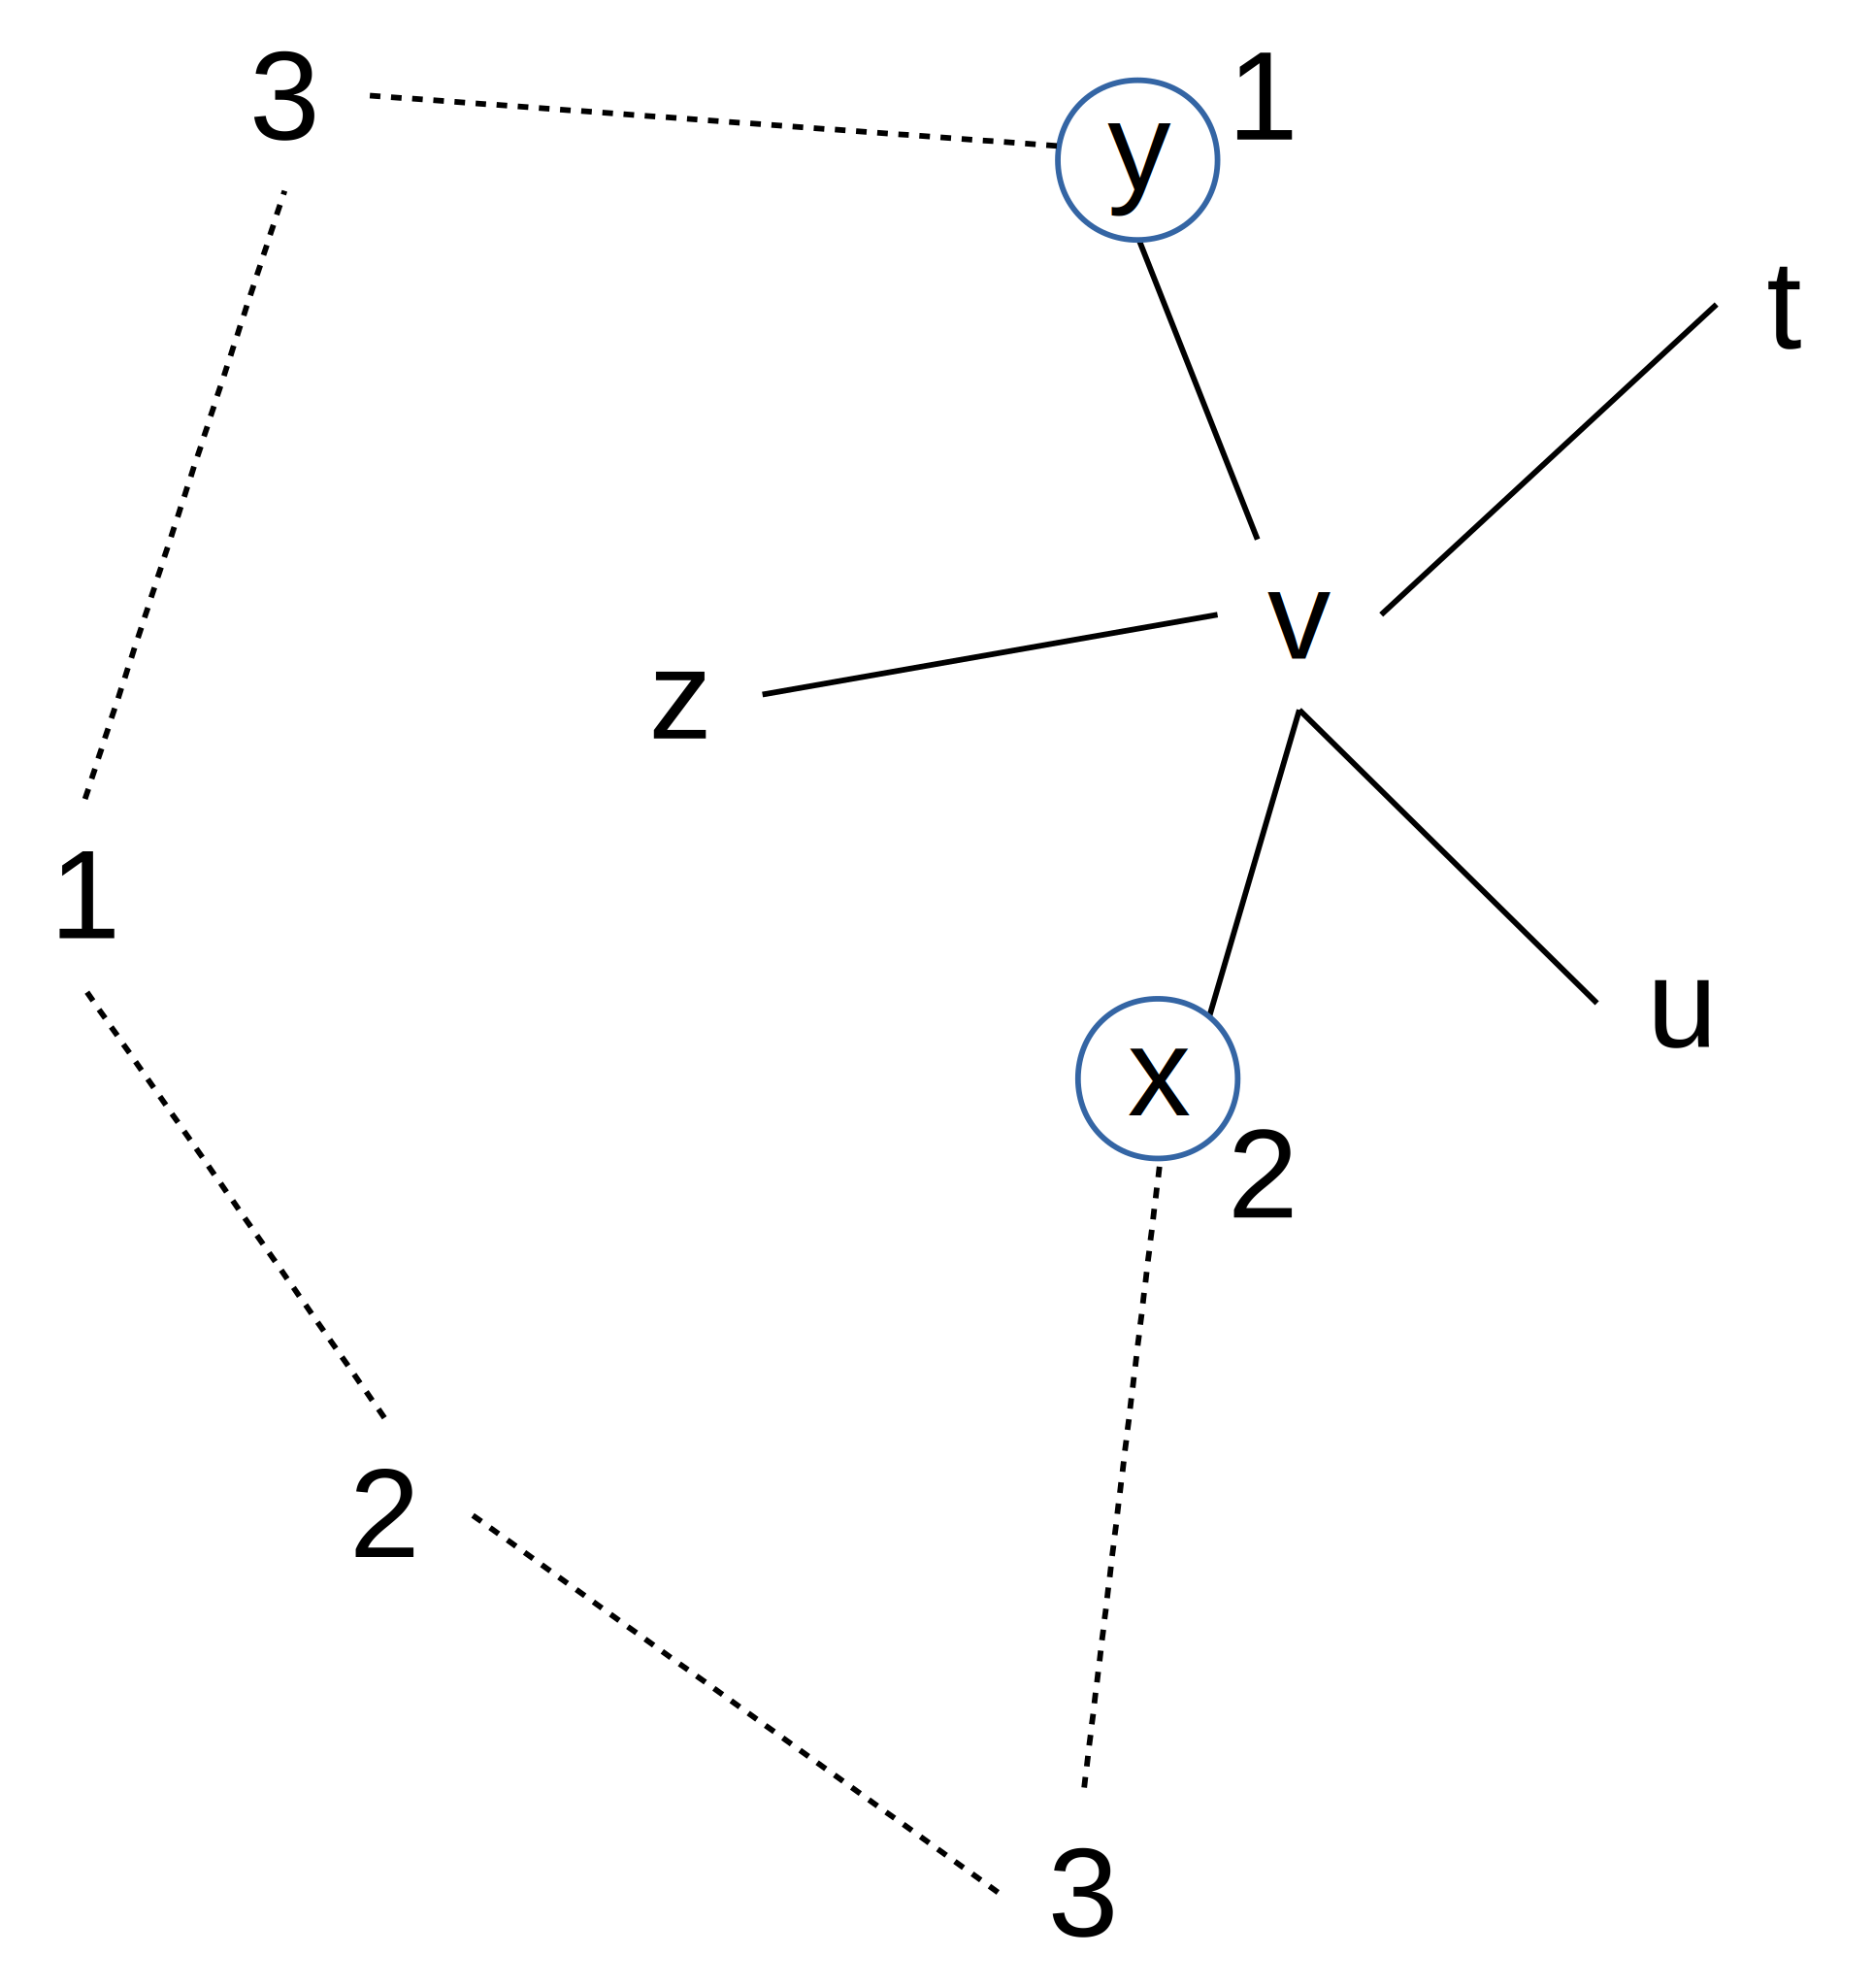
\includegraphics[scale=0.5]{lectures/161125/pix/2.pdf}
                        \begin{itemize}
                            \item betrachte 5-Färbung $\mathcal{C} \colon V(G \setminus \{v\}) \mapsto \{1, \dots, 5\}$, die es nach Rekursion gibt
                            \item betrache $x,y \in V_{xy}$ und sei $V_{xy} \subset V(G)$ die Menge der Knoten mit $\mathcal{C}(x)$- oder $\mathcal{C}(y)$-Färbung
                                \begin{enumerate}
                                    \item es gibt \underline{keinen} Weg von $x \rightsquigarrow y$, der nur Knoten aus $V_{xy}$ nutzt
                                        \begin{itemize}
                                            \item Seien $V'_{xy}$ die $s \in V(G \setminus \{v\})$, die von $x$ nur via $V_{xy}$ erreicht werden
                                            \item Färbe um:
                                            \begin{math}
                                                \mathcal{C'}(s) =
                                                    \begin{cases}
                                                        \mathcal{C}(s) & s \not \in V'_{xy}\\
                                                        \mathcal{C}(y) & s \in V'_{xy}, ~ \mathcal{C}(s) = \mathcal{C}(x)\\
                                                        \mathcal{C}(x) & s \in V'_{xy}, ~ \mathcal{C}(s) = \mathcal{C}(y)
                                                    \end{cases}
                                            \end{math}\\\\
                                            ``Tausche Farben auf $V'_{xy}$'' $\Rightarrow \mathcal{C'}(x) = \mathcal{C'}(y) = \mathcal{C}(y)$
                                        \end{itemize}
                                    \item es gibt einen solchen Pfad $x \rightsquigarrow y$ mit allen Knoten in $V_{xy}$
                                    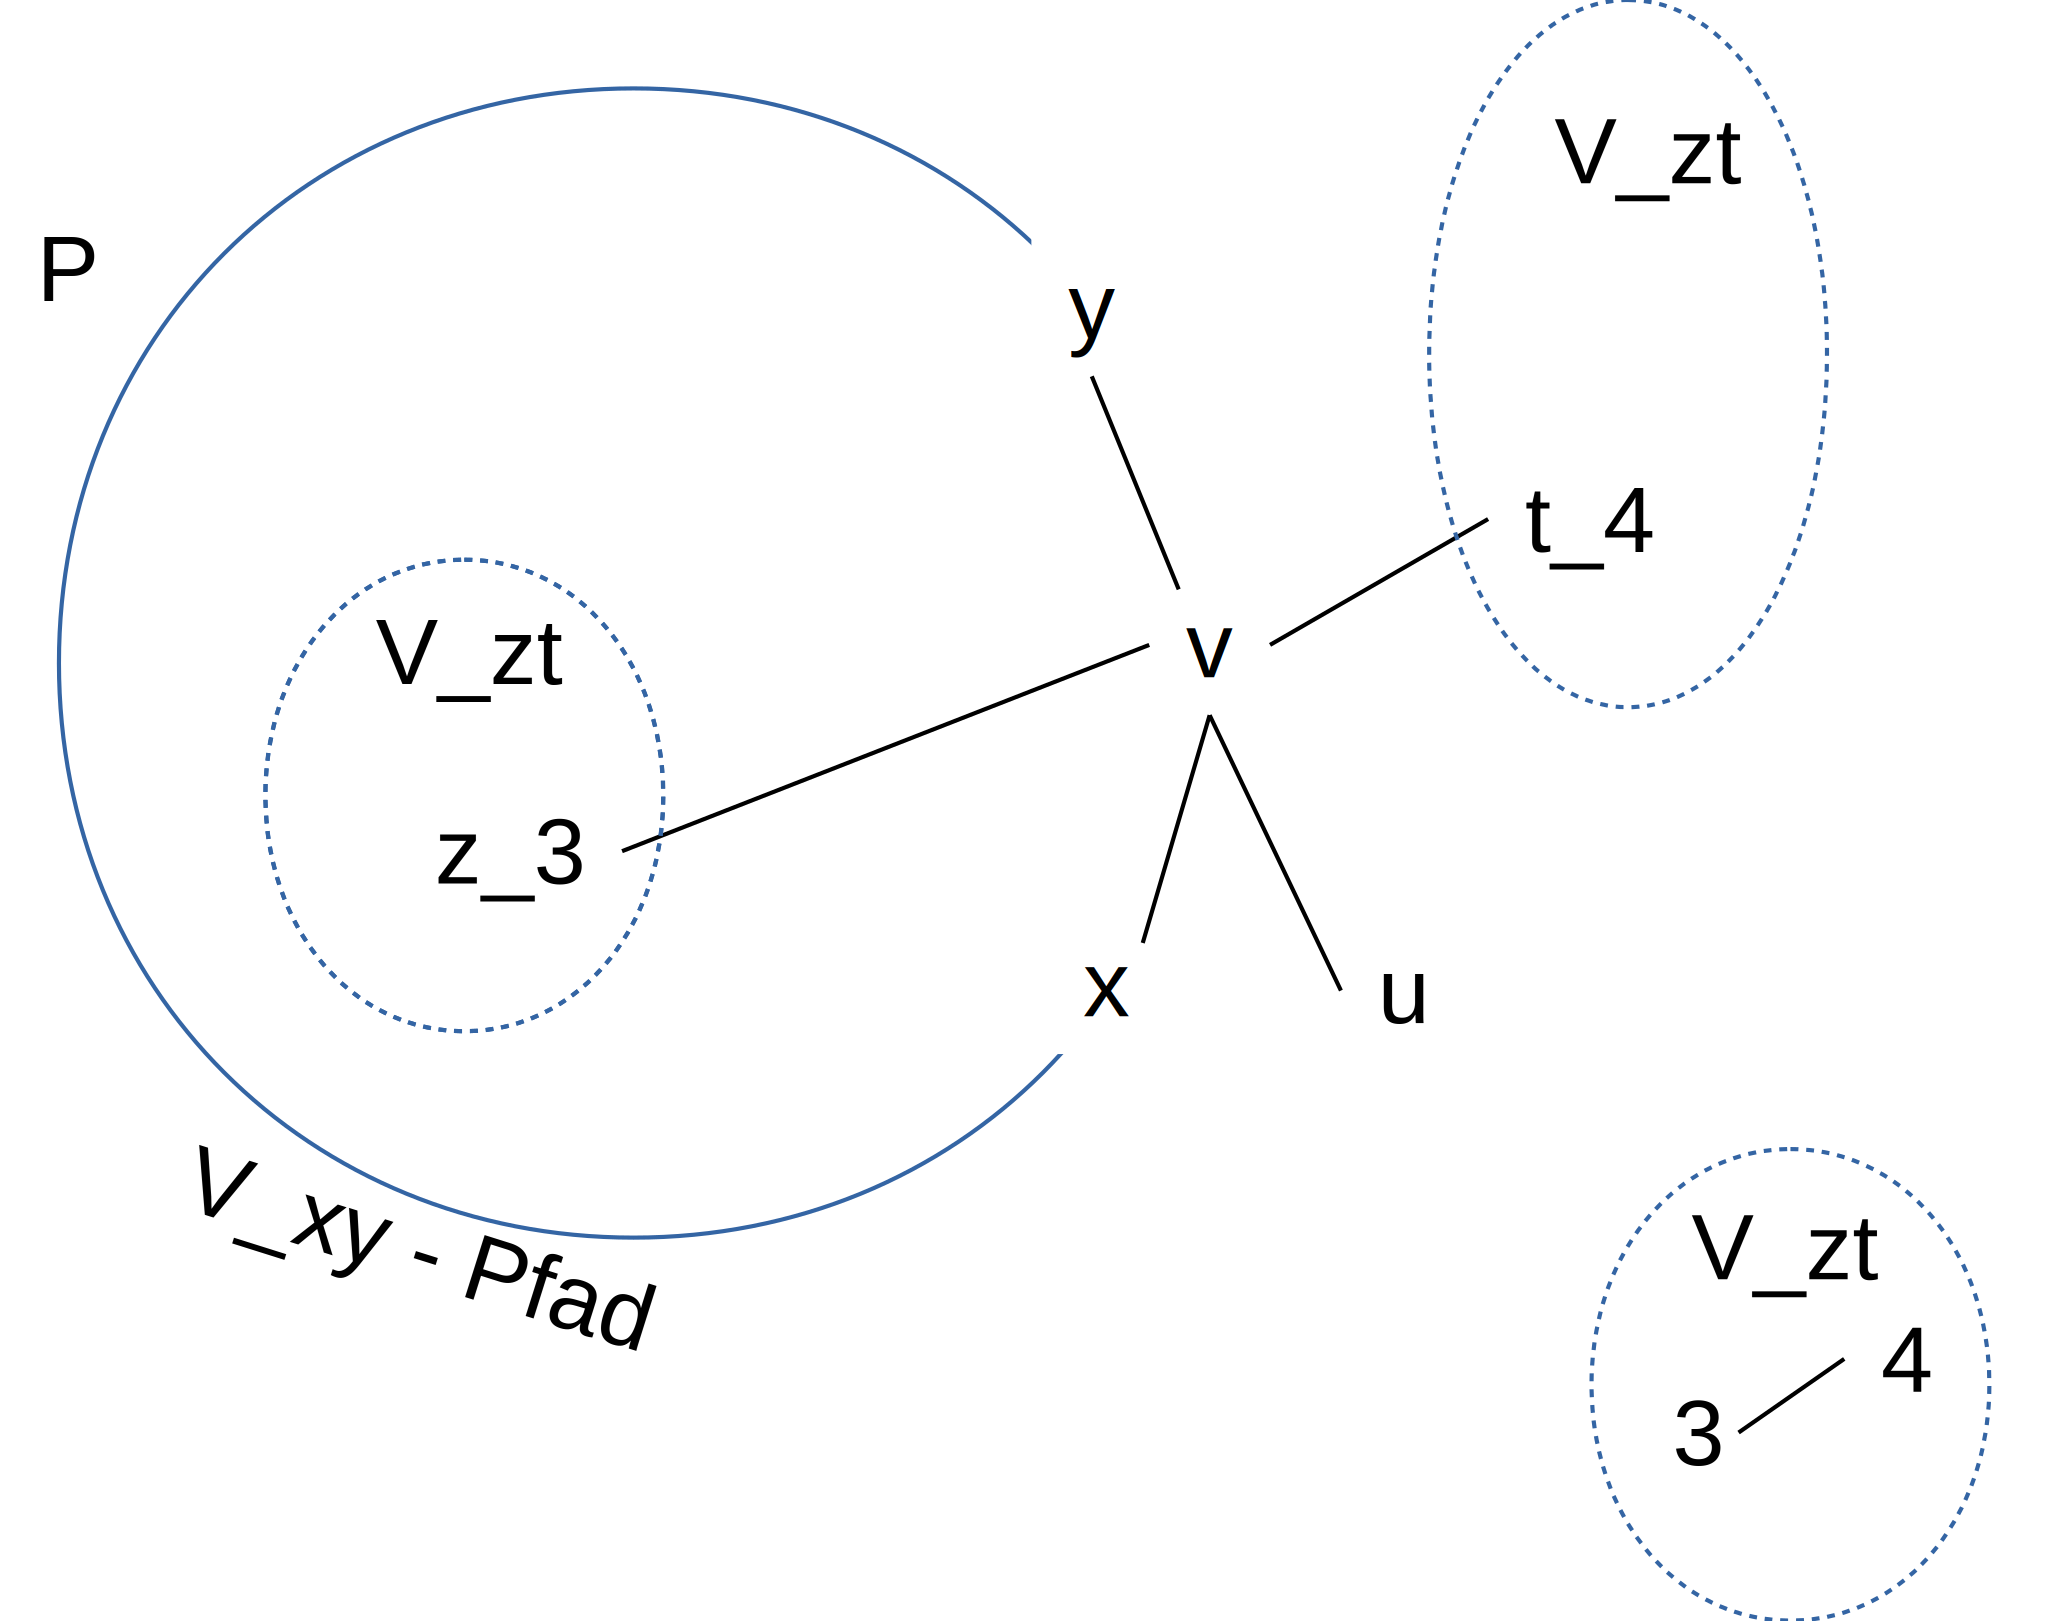
\includegraphics[scale=0.5]{lectures/161125/pix/3.pdf}
                                        \begin{itemize}
                                            \item $V_{zt}$: alle Knoten in $V(G \setminus \{v\})$, die $\mathcal{C}(t)$ oder $\mathcal{C}(z)$ gefärbt sind
                                            \item $V_{xy} \cap V_{zt} = \emptyset$!
                                            \item $V'_{zt}$ kann nur via eines $s \in P$ einen Knoten in $V_{zt} \setminus V'_{zt}$ erreichen
                                        \end{itemize}
                                        Damit lassen sich $z,t$ analog zu Fall (a) färben.
                                \end{enumerate}
                        \end{itemize}
                \end{enumerate}
        \end{description}
    \item[Theorem] Jeder planare Graph ist 4-färbbar
        \begin{description}
            \item[Proof] Es gibt eine Menge von 1936 4-färbbaren Karten, jede nicht Teil eines kleinsten Gegenbeispiels... (Appel, Haken, 1976).
            $\Rightarrow$ Es folgt, dass es kein kleinstes Gegenbeispiel gibt.
        \end{description}
\end{description}

\subsection{Zufallsgraphen}
Sei $G=(V,E)$ mit $V=\{1, \dots, n\}$ fixiert. Wir wollen nun Kanten zufällig auswählen auf dieser fixierten Kantenmenge $\{1, \dots, n\}$, um zufällige Graphen zu generieren. 
Die Menge dieser Zufallsgraphen nennen wir $\mathcal{G}$. \underline{Jede} Kante wird mit Wahrscheinlichkeit $p \in [0, \dots, 1]$ gewählt. 
Sei $G_0$ ein bestimmter Graph. Das Ereignis $\{G_0\}$ mit $G_0$ und m Kanten hat die Wahrscheinlichkeit $p^m \cdot (1-p)^{{n \over 2}-m}$. 
Wahrscheinlichkeitsmaß auf 
$\mathcal{G} ~ \forall e \in [v]^2$\\
$\Omega_e=\{0_e, 1_e\}$\\
$\mathbb{P}(\{1_e\})=p$\\
$\mathbb{P}(\{0_e\})=1-p$\\
$\Omega_\mathcal{G} = \prod\limits_{e \in [v]^2} \Omega_e$

\begin{description}
    \item[Beispiele] Fixiere Graph $H$, $V(H) = V(G)$, ist $H \leqslant G$? \\
        Mit $p^l$, $|E(H)| = l$, $|V(H)| = k$, aber falls $H$ induzierter Teilgraph von $G$ sein soll? \\
         - Nur $p^l (1-p)^{\binom{k}{2} - l}$. \\
        Und was ist mit Subgraph-Isomorphismus?
        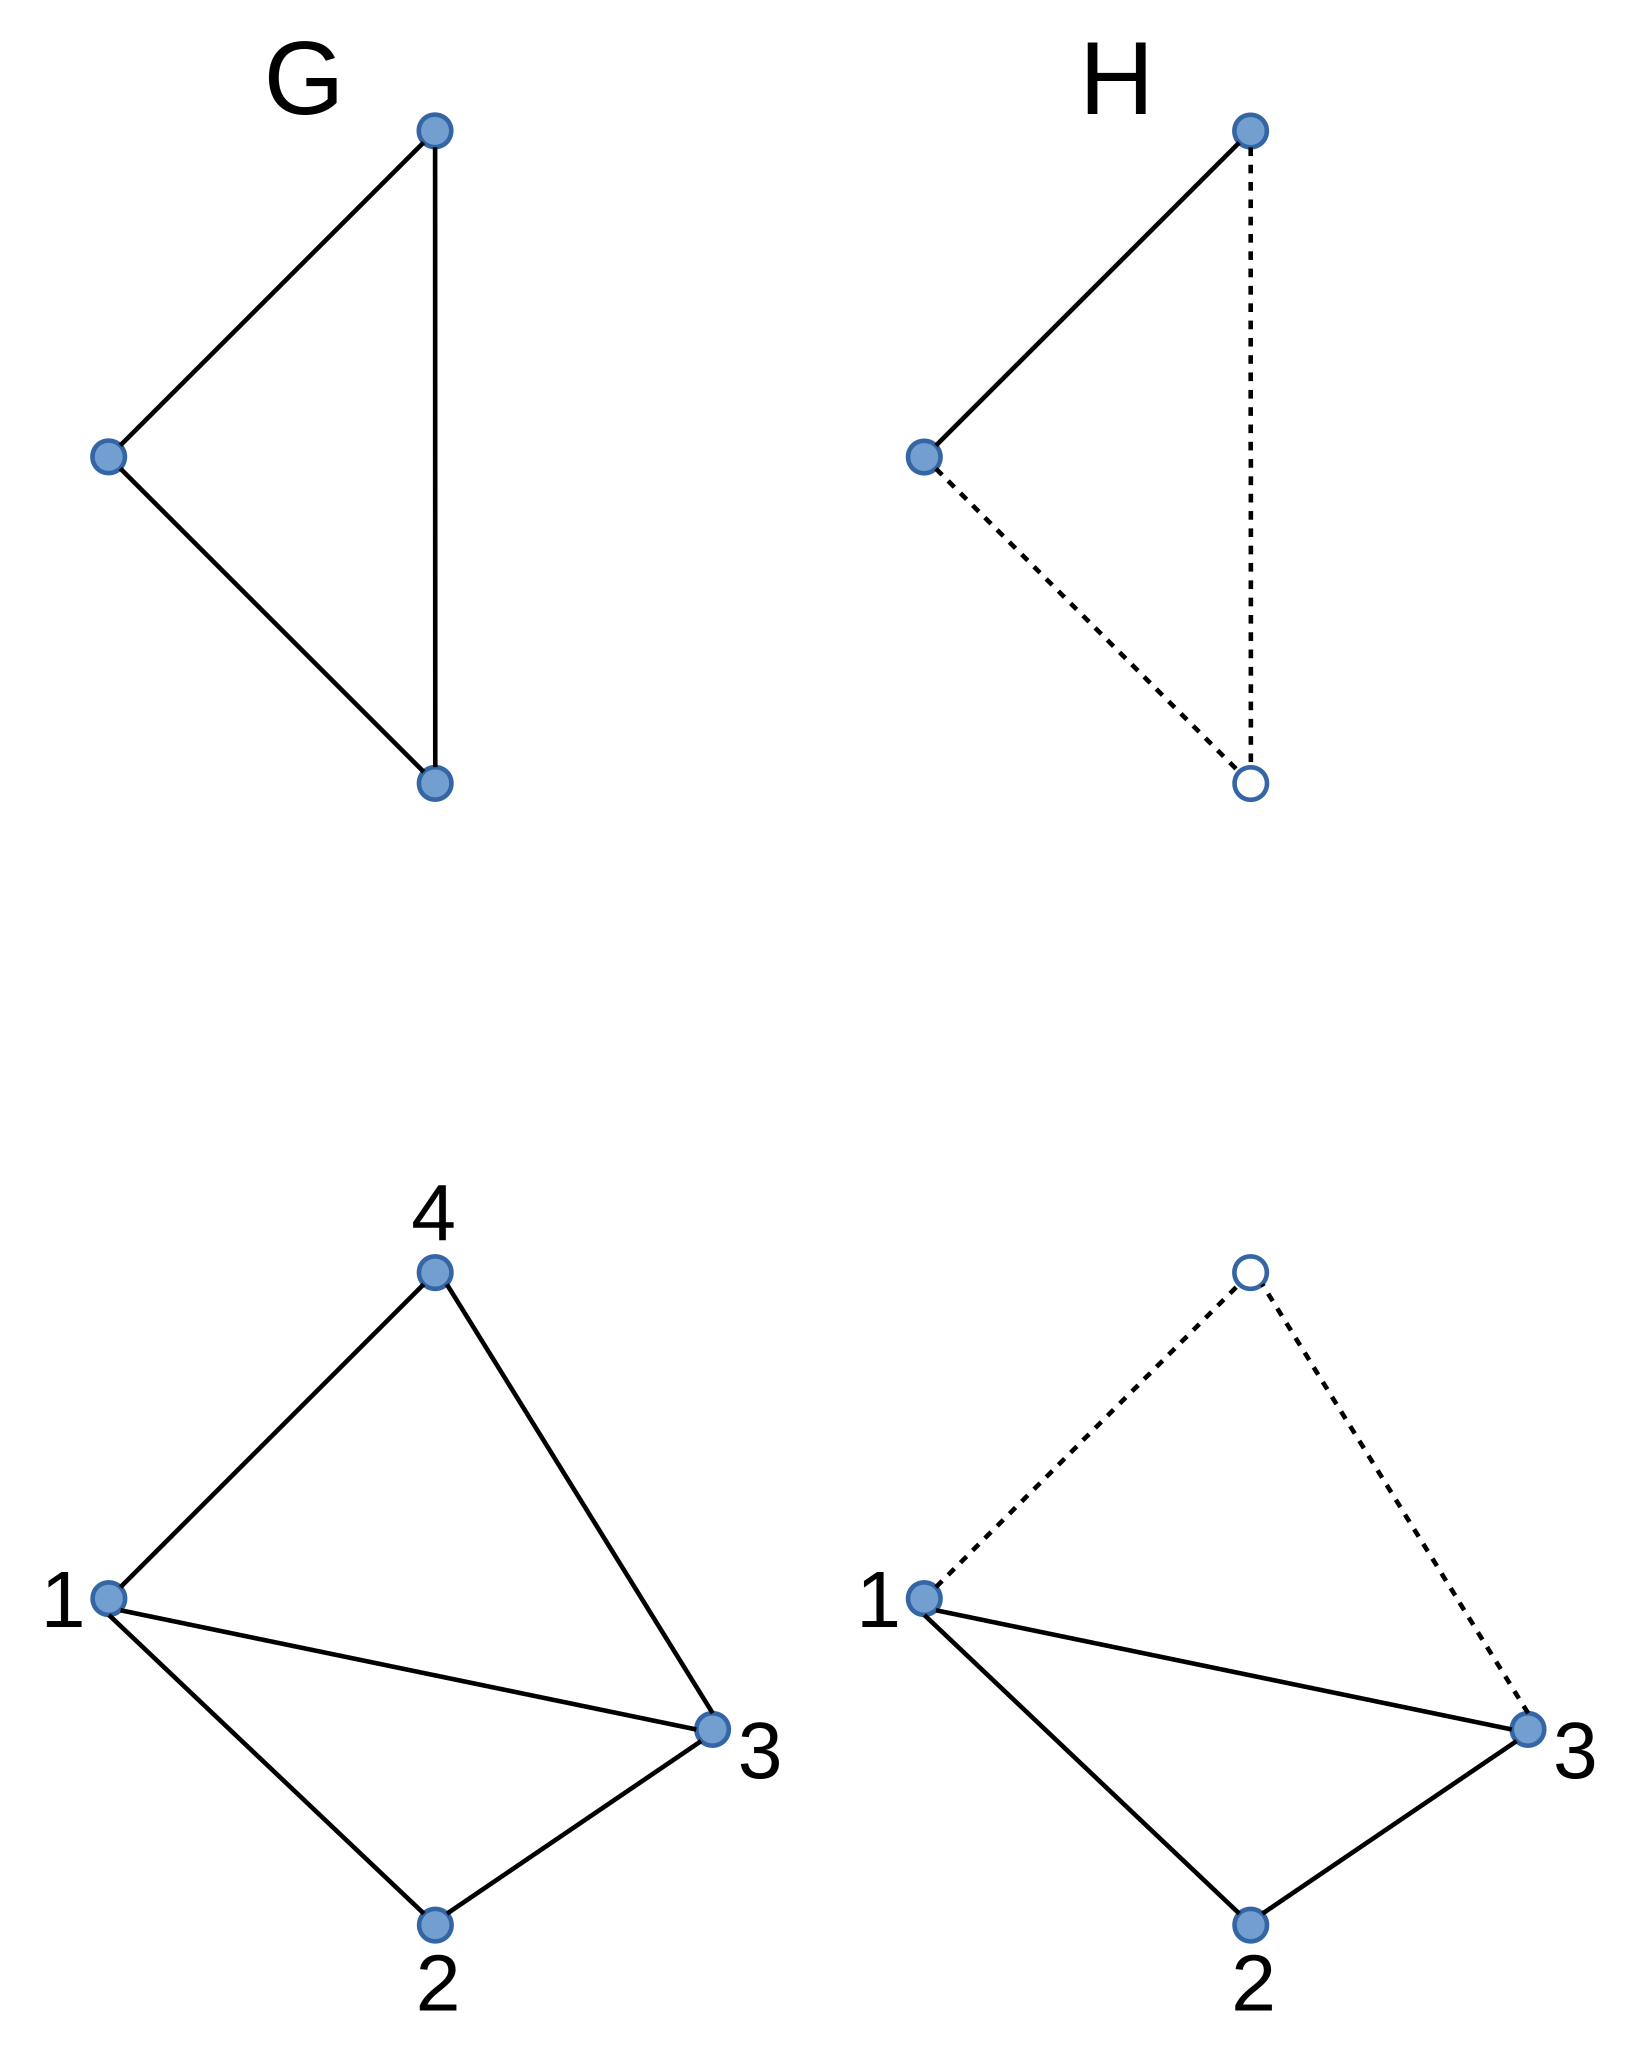
\includegraphics[scale=0.5]{lectures/161125/pix/4.pdf}
        \begin{itemize}
            \item Ereignismengen überlappen
            \item kompliziert
        \end{itemize}
\end{description}

\subsection{Eigenschaften fast aller Graphen}
Falls die Wahrscheinlichkeit, dass $P(G \in \mathcal{G}) \rightarrow 1$ für $n \rightarrow \infty$, dann geschieht $G$ fast sicher.
\begin{description}
    \item[Pro:] Gegeben jedes $H$ als Isomorphie-Klasse, $n \rightarrow \infty$ und $p \in ]0,1[ = (0,1)$, induzierte Kopie von $H$. 
    Dann haben fast alle $G$ in $\mathcal{G}(n,p)$ haben mindestens eine induzierte Kopie von $H$.
    \item[Prf:] Sei $H$ gegeben, $K=V(H)$. Sei $K \leqslant n$. $H$ ist (subgraph-) isomorph zu $G$ mit Wahrscheinlichkeit $r < 0$ ($G$ ist zufällig!). 
        Teile $G$ in $\lfloor {n \over k} \rfloor$ Teilgraphen, um genau so viele ``Versuche'' (für $r > 0$) zu haben. 
        $P(H \not \subseteq G$ induziert) $\leqslant (1-r)^{\lfloor {n \over k} \rfloor} \xrightarrow{n \rightarrow \infty} 0$
\end{description}


\newpage

\section{Vorlesung 25.11.2016}
\subsection{Färbung von Graphen}
\subsubsection{Vertexfärbung}
Zwei durch eine Kante verbundene Knoten haben unterschiedliche Farben.\\
Beispiel wäre eine Landkarte auf der mit so wenig wie möglich Farben die Länder ausgemalt werden, ohne zwei benachbarte Länder gleichfarbig zu haben. Hierbei entspricht jede Facette einen Knoten.\\
\includegraphics[width=0.4\textwidth]{lectures/161125/pix/Vertexfaerbung}
\begin{description}
    \item[Vertexfärbung] Eine Vertexfärbung eines Graphen $G=(V,E)$ ist eine Abbildung $\mathcal{C} \colon V \mapsto \mathcal{S}$, mit $\mathcal{S}=$ Menge der Farben. Es gilt, dass $\mathcal{C}(v) \neq \mathcal{C}(w)$, mit $w,v \in \mathcal{S}$, wenn $v$ und $w$ adjazent ($\{v,w\} \in E$) sind. Die Elemente von $\mathcal{S}$ heißen \emph{Farben}.
    \item[k-Färbung] Ein Graph $G$ ist $k$-färbbar, wenn es für eine Abbildung $\mathcal{C}$ eine Menge $\mathcal{S}=\{1,\dots,k\}$ gibt.
    \item[Chromatische Zahl] Eine chromatische Zahl $\chi(G)$ ist die kleinste natürliche Zahl $k$, sodass G $k$-färbbar ist. $\chi(G) \leqslant \Delta(G) + 1$, mit $\Delta(G) = $ maximaler Grad von $G$
        \begin{description}
            \item[Proof (greedy)] Färbe $v_i$ der Vertices $v_1 \dots v_n$ mit der kleinsten Farbe, die nicht von einem Nachbarn von $v_i$ benutzt wird. Da wir max. $\Delta(G)$ viele Nachbarn für $v_i$ haben, gibt es immer eine freie Farbe.
        \end{description}
        $\chi(G) \geqslant$ Größe der größten Clique
    \item[Lemma] Für jeden einfachen planaren Graphen $G$ ist der Durchschnittsgrad $d(G) < 6$
        \begin{description}
            \item[Proof] $d(G) = 2 \cdot {|E| \over |V|}$ mit $|V| \leqslant 3$, $|E| \leqslant 3  \cdot |V| - 6$, dann $d(G) \leqslant {2(3 \cdot |V|-6) \over |V|} = 6-{12 \over |V|}$
        \end{description}
    \item[Theorem] Jeder simple planare Graph $G$ hat $\chi(G) \leqslant 6$
        \begin{description}
            \item[Proof] Annahme: Jeder simple planare Graph mit $|V| = n$ ist $6$-färbbar.
            \begin{itemize}
                \item Sei $G$ hiermit ein simpler planarer Graph mit $|V| = n+1$
                \item Vom Lemma wissen wir, dass $w \in V$ mit $d(w) \leqslant 5$ existiert
                \item Sei $G' = G \setminus \{w\}$. Via Induktionshypothese ist $G'$ 6-färbbar. Das tun wir dann.
                \item Färbe $w$ mit der (min.) freien Farbe, um $G$ zu färben
            \end{itemize}
        \end{description}
    \item[Theorem] Für jeden simplen planaren Graphen $G$ gilt, dass $\chi(G) \leqslant 5$
        \begin{description}
            \item[Proof] Sei $G=(V,E)$ planar
                \begin{enumerate}
                    \item Falls $|V| \leqslant 5 \rightarrow$ trivial
                    \item Für alle $v \in V(G)$ mit $deg(v) < 5$, färbe $v$ und arbeite mit $G \setminus \{v\}$
                    \item $G$ hat Vertex $v$ mit $deg(v) = 5$
                        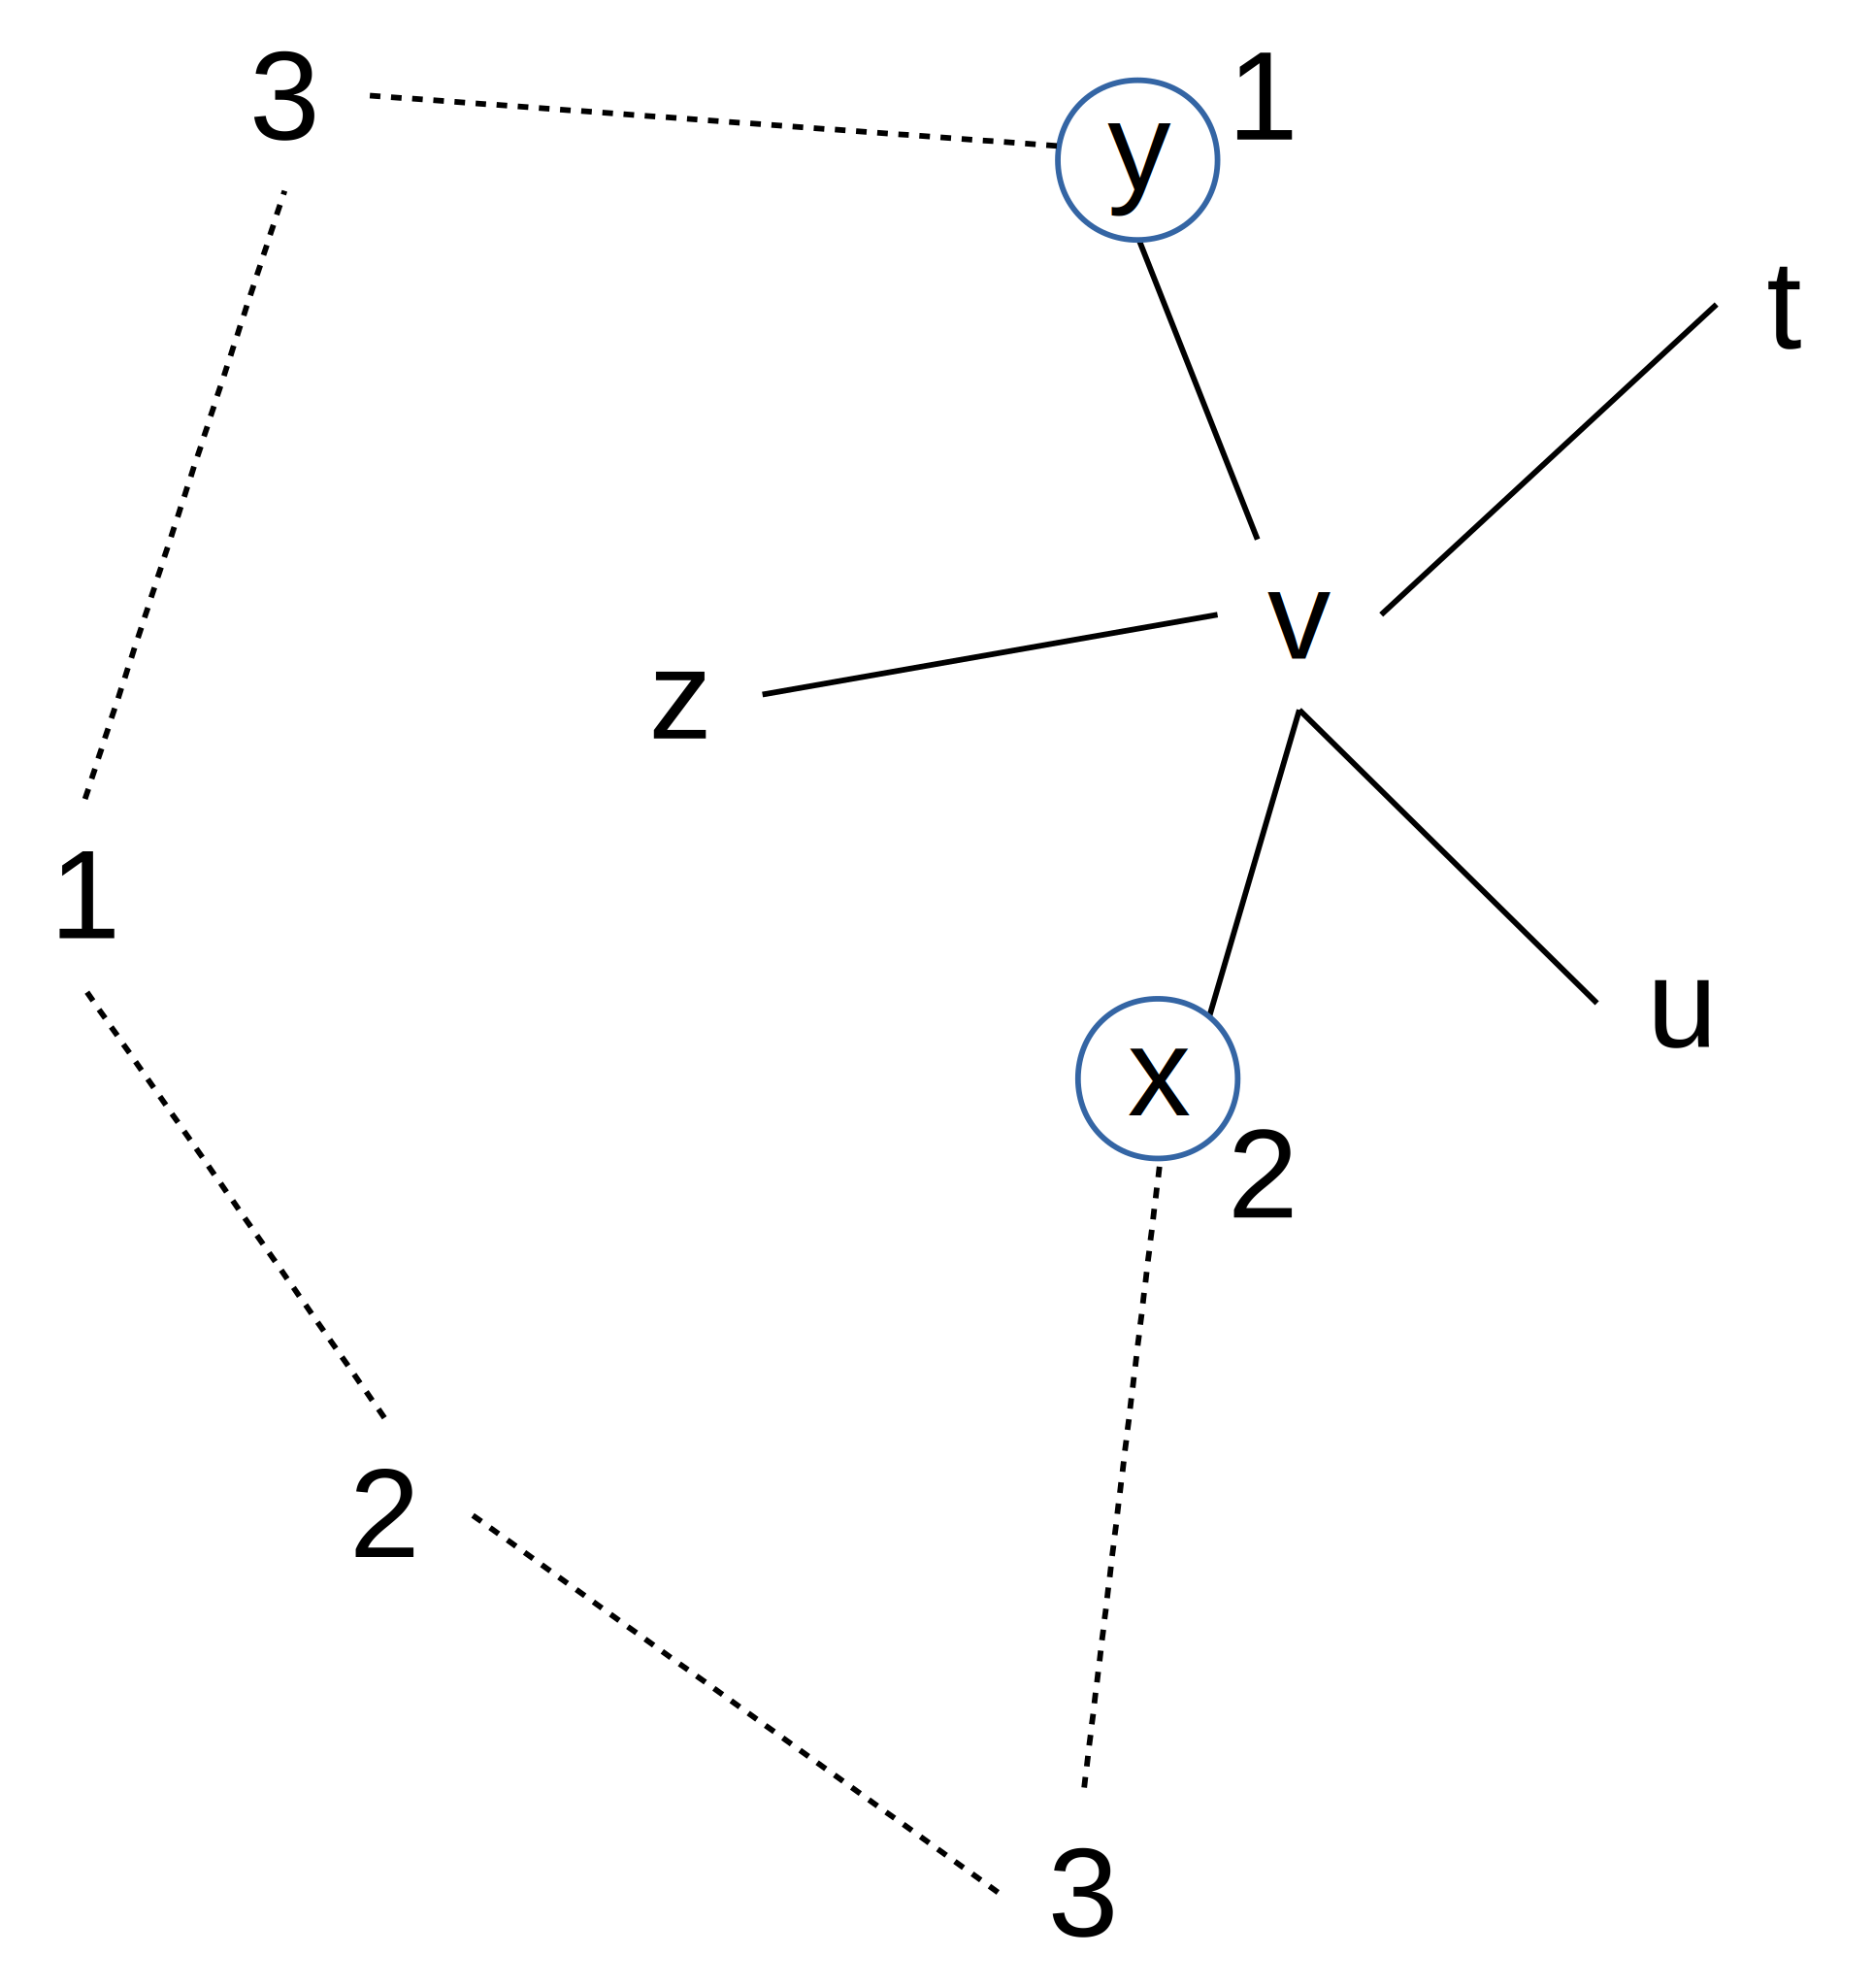
\includegraphics[scale=0.5]{lectures/161125/pix/2.pdf}
                        \begin{itemize}
                            \item betrachte 5-Färbung $\mathcal{C} \colon V(G \setminus \{v\}) \mapsto \{1, \dots, 5\}$, die es nach Rekursion gibt
                            \item betrache $x,y \in V_{xy}$ und sei $V_{xy} \subset V(G)$ die Menge der Knoten mit $\mathcal{C}(x)$- oder $\mathcal{C}(y)$-Färbung
                                \begin{enumerate}
                                    \item es gibt \underline{keinen} Weg von $x \rightsquigarrow y$, der nur Knoten aus $V_{xy}$ nutzt
                                        \begin{itemize}
                                            \item Seien $V'_{xy}$ die $s \in V(G \setminus \{v\})$, die von $x$ nur via $V_{xy}$ erreicht werden
                                            \item Färbe um:
                                            \begin{math}
                                                \mathcal{C'}(s) =
                                                    \begin{cases}
                                                        \mathcal{C}(s) & s \not \in V'_{xy}\\
                                                        \mathcal{C}(y) & s \in V'_{xy}, ~ \mathcal{C}(s) = \mathcal{C}(x)\\
                                                        \mathcal{C}(x) & s \in V'_{xy}, ~ \mathcal{C}(s) = \mathcal{C}(y)
                                                    \end{cases}
                                            \end{math}\\\\
                                            ``Tausche Farben auf $V'_{xy}$'' $\Rightarrow \mathcal{C'}(x) = \mathcal{C'}(y) = \mathcal{C}(y)$
                                        \end{itemize}
                                    \item es gibt einen solchen Pfad $x \rightsquigarrow y$ mit allen Knoten in $V_{xy}$
                                    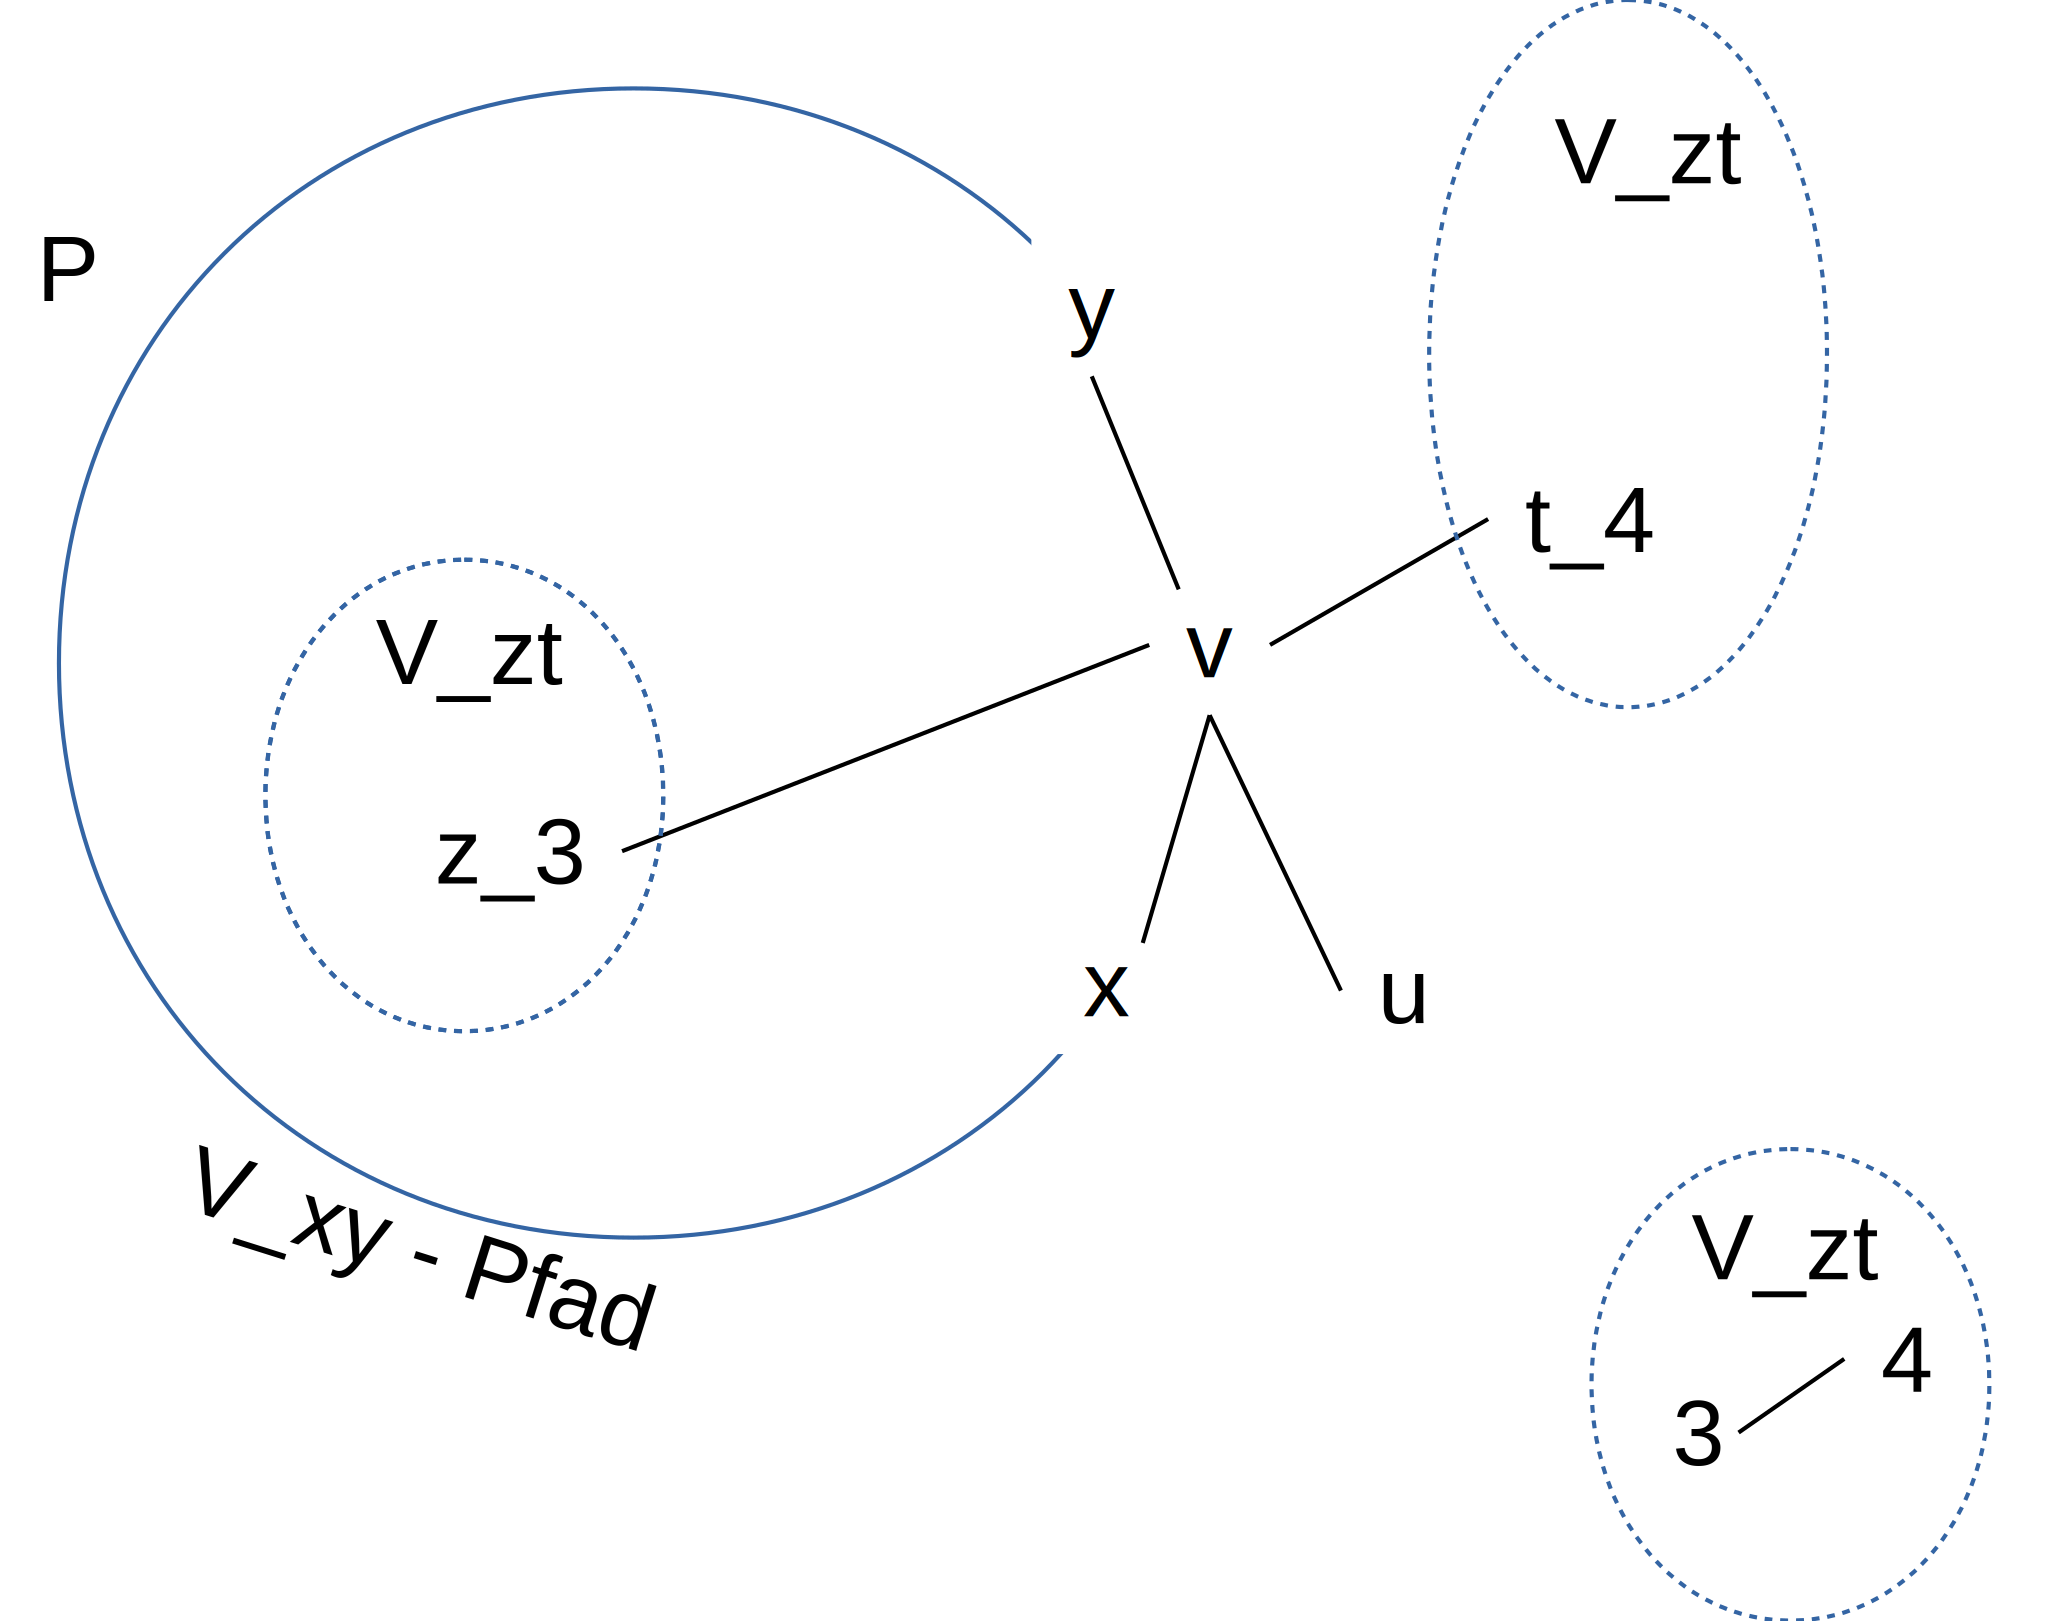
\includegraphics[scale=0.5]{lectures/161125/pix/3.pdf}
                                        \begin{itemize}
                                            \item $V_{zt}$: alle Knoten in $V(G \setminus \{v\})$, die $\mathcal{C}(t)$ oder $\mathcal{C}(z)$ gefärbt sind
                                            \item $V_{xy} \cap V_{zt} = \emptyset$!
                                            \item $V'_{zt}$ kann nur via eines $s \in P$ einen Knoten in $V_{zt} \setminus V'_{zt}$ erreichen
                                        \end{itemize}
                                        Damit lassen sich $z,t$ analog zu Fall (a) färben.
                                \end{enumerate}
                        \end{itemize}
                \end{enumerate}
        \end{description}
    \item[Theorem] Jeder planare Graph ist 4-färbbar
        \begin{description}
            \item[Proof] Es gibt eine Menge von 1936 4-färbbaren Karten, jede nicht Teil eines kleinsten Gegenbeispiels... (Appel, Haken, 1976).
            $\Rightarrow$ Es folgt, dass es kein kleinstes Gegenbeispiel gibt.
        \end{description}
\end{description}

\subsection{Zufallsgraphen}
Sei $G=(V,E)$ mit $V=\{1, \dots, n\}$ fixiert. Wir wollen nun Kanten zufällig auswählen auf dieser fixierten Kantenmenge $\{1, \dots, n\}$, um zufällige Graphen zu generieren. 
Die Menge dieser Zufallsgraphen nennen wir $\mathcal{G}$. \underline{Jede} Kante wird mit Wahrscheinlichkeit $p \in [0, \dots, 1]$ gewählt. 
Sei $G_0$ ein bestimmter Graph. Das Ereignis $\{G_0\}$ mit $G_0$ und m Kanten hat die Wahrscheinlichkeit $p^m \cdot (1-p)^{{n \over 2}-m}$. 
Wahrscheinlichkeitsmaß auf 
$\mathcal{G} ~ \forall e \in [v]^2$\\
$\Omega_e=\{0_e, 1_e\}$\\
$\mathbb{P}(\{1_e\})=p$\\
$\mathbb{P}(\{0_e\})=1-p$\\
$\Omega_\mathcal{G} = \prod\limits_{e \in [v]^2} \Omega_e$

\begin{description}
    \item[Beispiele] Fixiere Graph $H$, $V(H) = V(G)$, ist $H \leqslant G$? \\
        Mit $p^l$, $|E(H)| = l$, $|V(H)| = k$, aber falls $H$ induzierter Teilgraph von $G$ sein soll? \\
         - Nur $p^l (1-p)^{\binom{k}{2} - l}$. \\
        Und was ist mit Subgraph-Isomorphismus?
        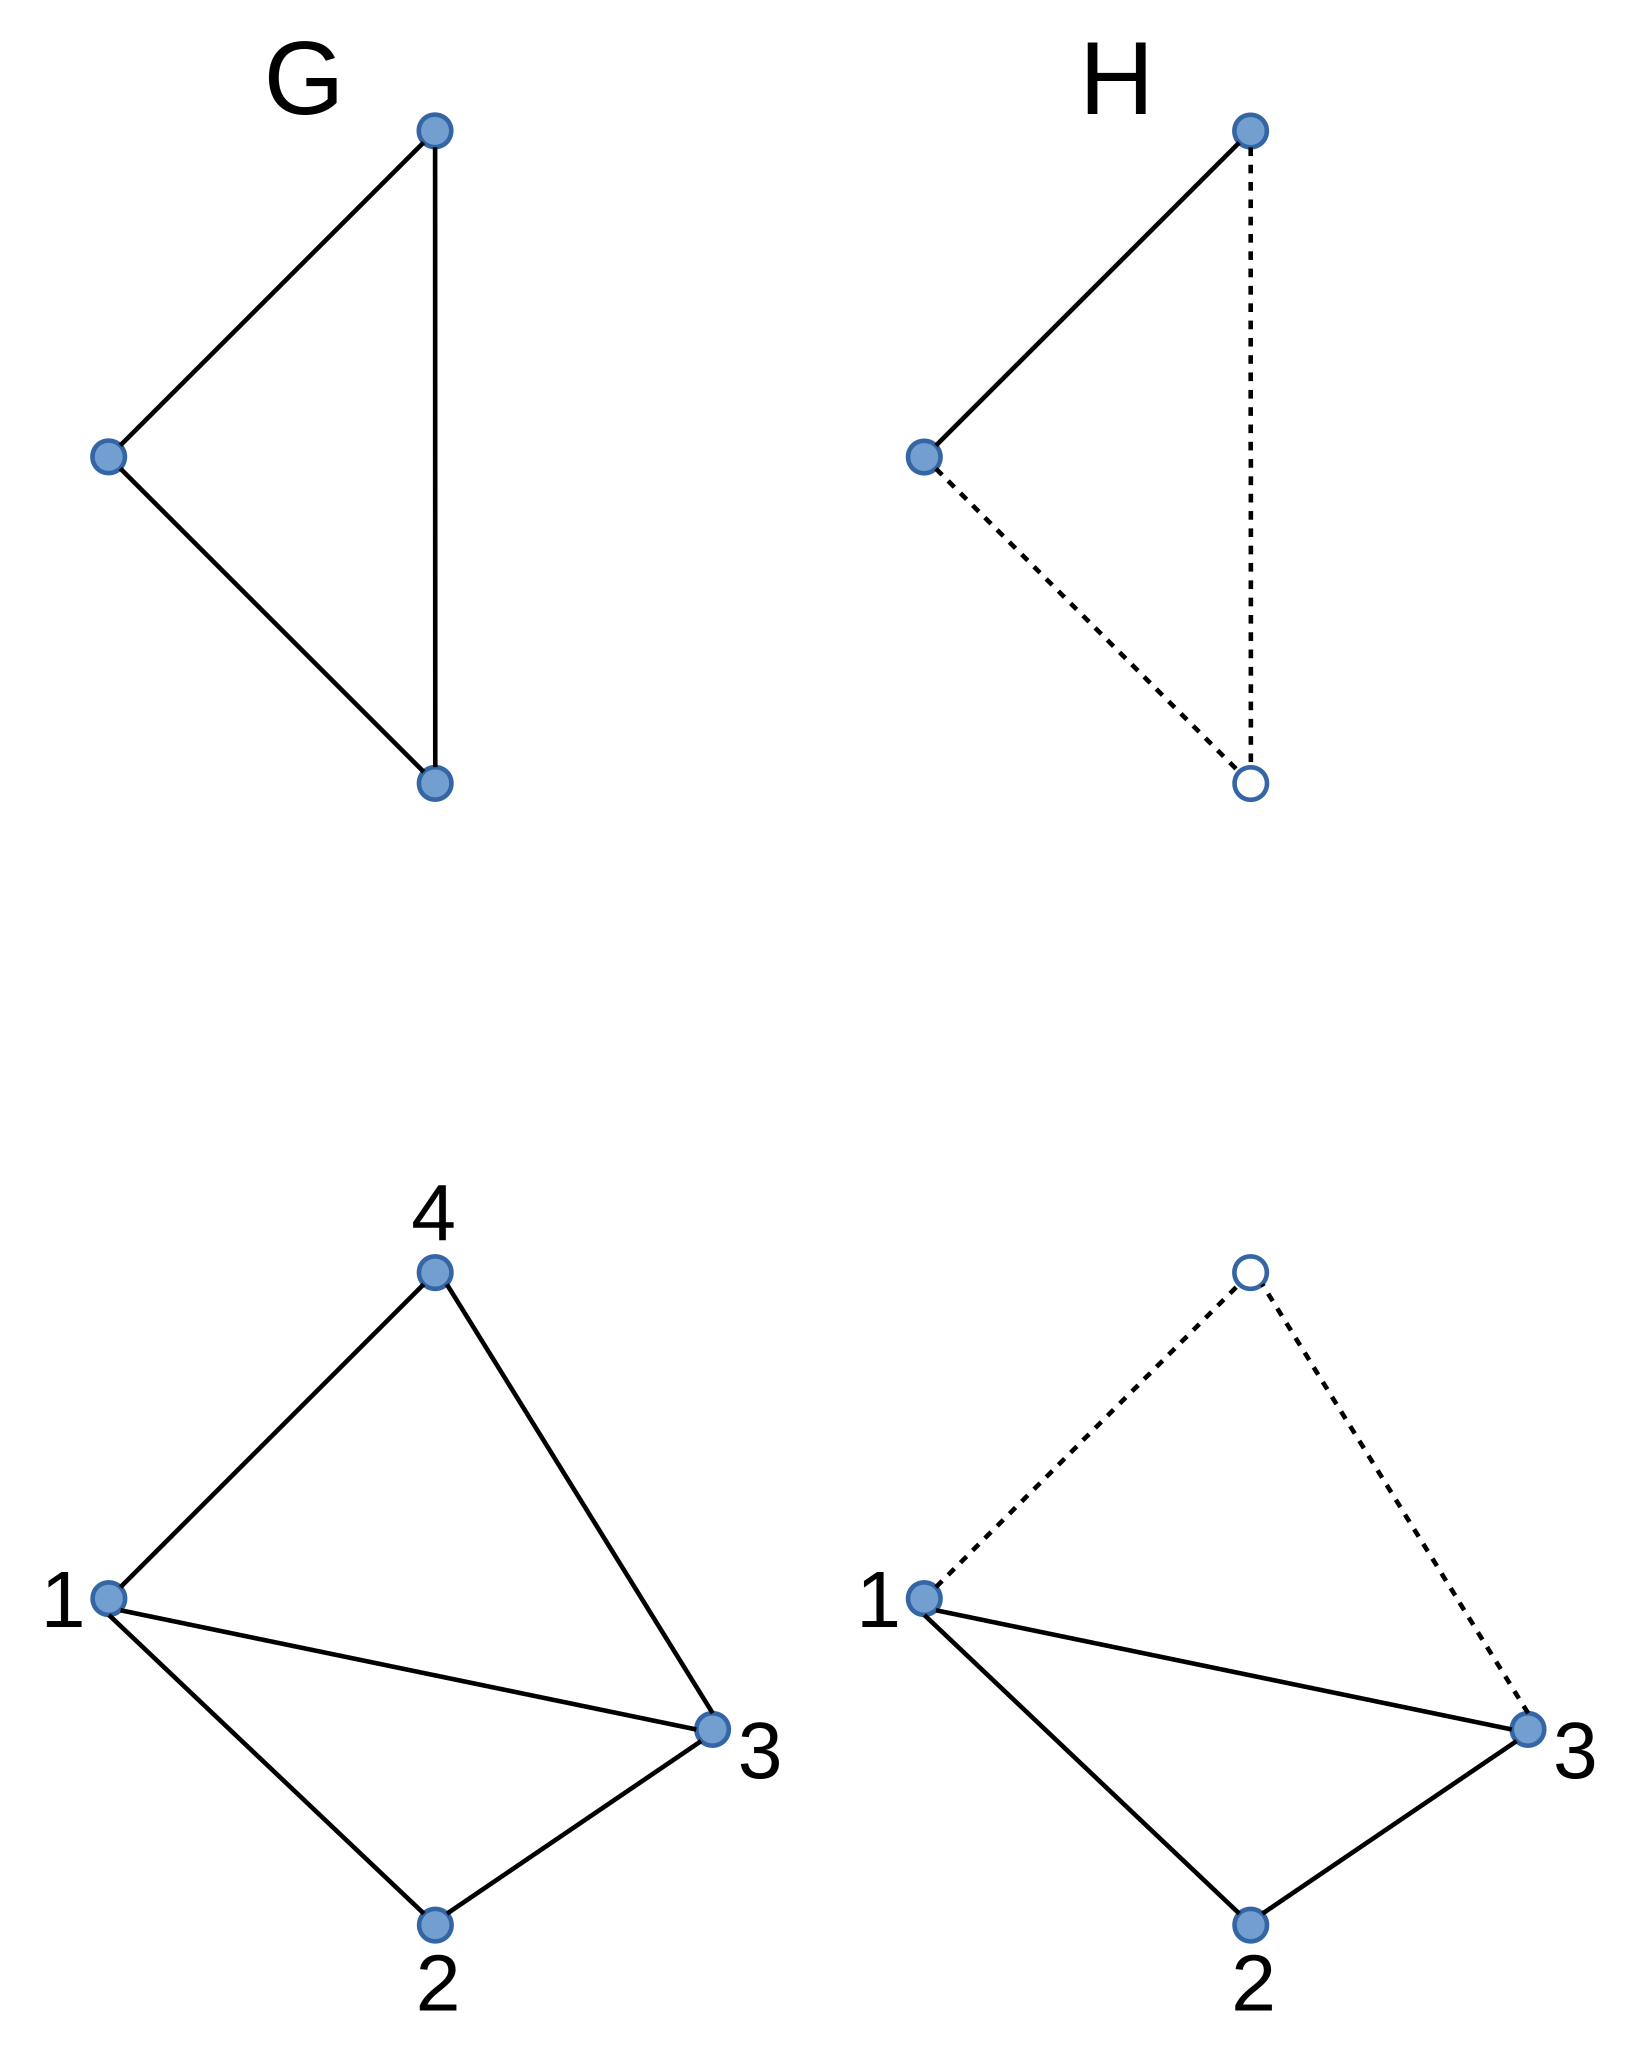
\includegraphics[scale=0.5]{lectures/161125/pix/4.pdf}
        \begin{itemize}
            \item Ereignismengen überlappen
            \item kompliziert
        \end{itemize}
\end{description}

\subsection{Eigenschaften fast aller Graphen}
Falls die Wahrscheinlichkeit, dass $P(G \in \mathcal{G}) \rightarrow 1$ für $n \rightarrow \infty$, dann geschieht $G$ fast sicher.
\begin{description}
    \item[Pro:] Gegeben jedes $H$ als Isomorphie-Klasse, $n \rightarrow \infty$ und $p \in ]0,1[ = (0,1)$, induzierte Kopie von $H$. 
    Dann haben fast alle $G$ in $\mathcal{G}(n,p)$ haben mindestens eine induzierte Kopie von $H$.
    \item[Prf:] Sei $H$ gegeben, $K=V(H)$. Sei $K \leqslant n$. $H$ ist (subgraph-) isomorph zu $G$ mit Wahrscheinlichkeit $r < 0$ ($G$ ist zufällig!). 
        Teile $G$ in $\lfloor {n \over k} \rfloor$ Teilgraphen, um genau so viele ``Versuche'' (für $r > 0$) zu haben. 
        $P(H \not \subseteq G$ induziert) $\leqslant (1-r)^{\lfloor {n \over k} \rfloor} \xrightarrow{n \rightarrow \infty} 0$
\end{description}


\newpage

\section{Vorlesung 25.11.2016}
\subsection{Färbung von Graphen}
\subsubsection{Vertexfärbung}
Zwei durch eine Kante verbundene Knoten haben unterschiedliche Farben.\\
Beispiel wäre eine Landkarte auf der mit so wenig wie möglich Farben die Länder ausgemalt werden, ohne zwei benachbarte Länder gleichfarbig zu haben. Hierbei entspricht jede Facette einen Knoten.\\
\includegraphics[width=0.4\textwidth]{lectures/161125/pix/Vertexfaerbung}
\begin{description}
    \item[Vertexfärbung] Eine Vertexfärbung eines Graphen $G=(V,E)$ ist eine Abbildung $\mathcal{C} \colon V \mapsto \mathcal{S}$, mit $\mathcal{S}=$ Menge der Farben. Es gilt, dass $\mathcal{C}(v) \neq \mathcal{C}(w)$, mit $w,v \in \mathcal{S}$, wenn $v$ und $w$ adjazent ($\{v,w\} \in E$) sind. Die Elemente von $\mathcal{S}$ heißen \emph{Farben}.
    \item[k-Färbung] Ein Graph $G$ ist $k$-färbbar, wenn es für eine Abbildung $\mathcal{C}$ eine Menge $\mathcal{S}=\{1,\dots,k\}$ gibt.
    \item[Chromatische Zahl] Eine chromatische Zahl $\chi(G)$ ist die kleinste natürliche Zahl $k$, sodass G $k$-färbbar ist. $\chi(G) \leqslant \Delta(G) + 1$, mit $\Delta(G) = $ maximaler Grad von $G$
        \begin{description}
            \item[Proof (greedy)] Färbe $v_i$ der Vertices $v_1 \dots v_n$ mit der kleinsten Farbe, die nicht von einem Nachbarn von $v_i$ benutzt wird. Da wir max. $\Delta(G)$ viele Nachbarn für $v_i$ haben, gibt es immer eine freie Farbe.
        \end{description}
        $\chi(G) \geqslant$ Größe der größten Clique
    \item[Lemma] Für jeden einfachen planaren Graphen $G$ ist der Durchschnittsgrad $d(G) < 6$
        \begin{description}
            \item[Proof] $d(G) = 2 \cdot {|E| \over |V|}$ mit $|V| \leqslant 3$, $|E| \leqslant 3  \cdot |V| - 6$, dann $d(G) \leqslant {2(3 \cdot |V|-6) \over |V|} = 6-{12 \over |V|}$
        \end{description}
    \item[Theorem] Jeder simple planare Graph $G$ hat $\chi(G) \leqslant 6$
        \begin{description}
            \item[Proof] Annahme: Jeder simple planare Graph mit $|V| = n$ ist $6$-färbbar.
            \begin{itemize}
                \item Sei $G$ hiermit ein simpler planarer Graph mit $|V| = n+1$
                \item Vom Lemma wissen wir, dass $w \in V$ mit $d(w) \leqslant 5$ existiert
                \item Sei $G' = G \setminus \{w\}$. Via Induktionshypothese ist $G'$ 6-färbbar. Das tun wir dann.
                \item Färbe $w$ mit der (min.) freien Farbe, um $G$ zu färben
            \end{itemize}
        \end{description}
    \item[Theorem] Für jeden simplen planaren Graphen $G$ gilt, dass $\chi(G) \leqslant 5$
        \begin{description}
            \item[Proof] Sei $G=(V,E)$ planar
                \begin{enumerate}
                    \item Falls $|V| \leqslant 5 \rightarrow$ trivial
                    \item Für alle $v \in V(G)$ mit $deg(v) < 5$, färbe $v$ und arbeite mit $G \setminus \{v\}$
                    \item $G$ hat Vertex $v$ mit $deg(v) = 5$
                        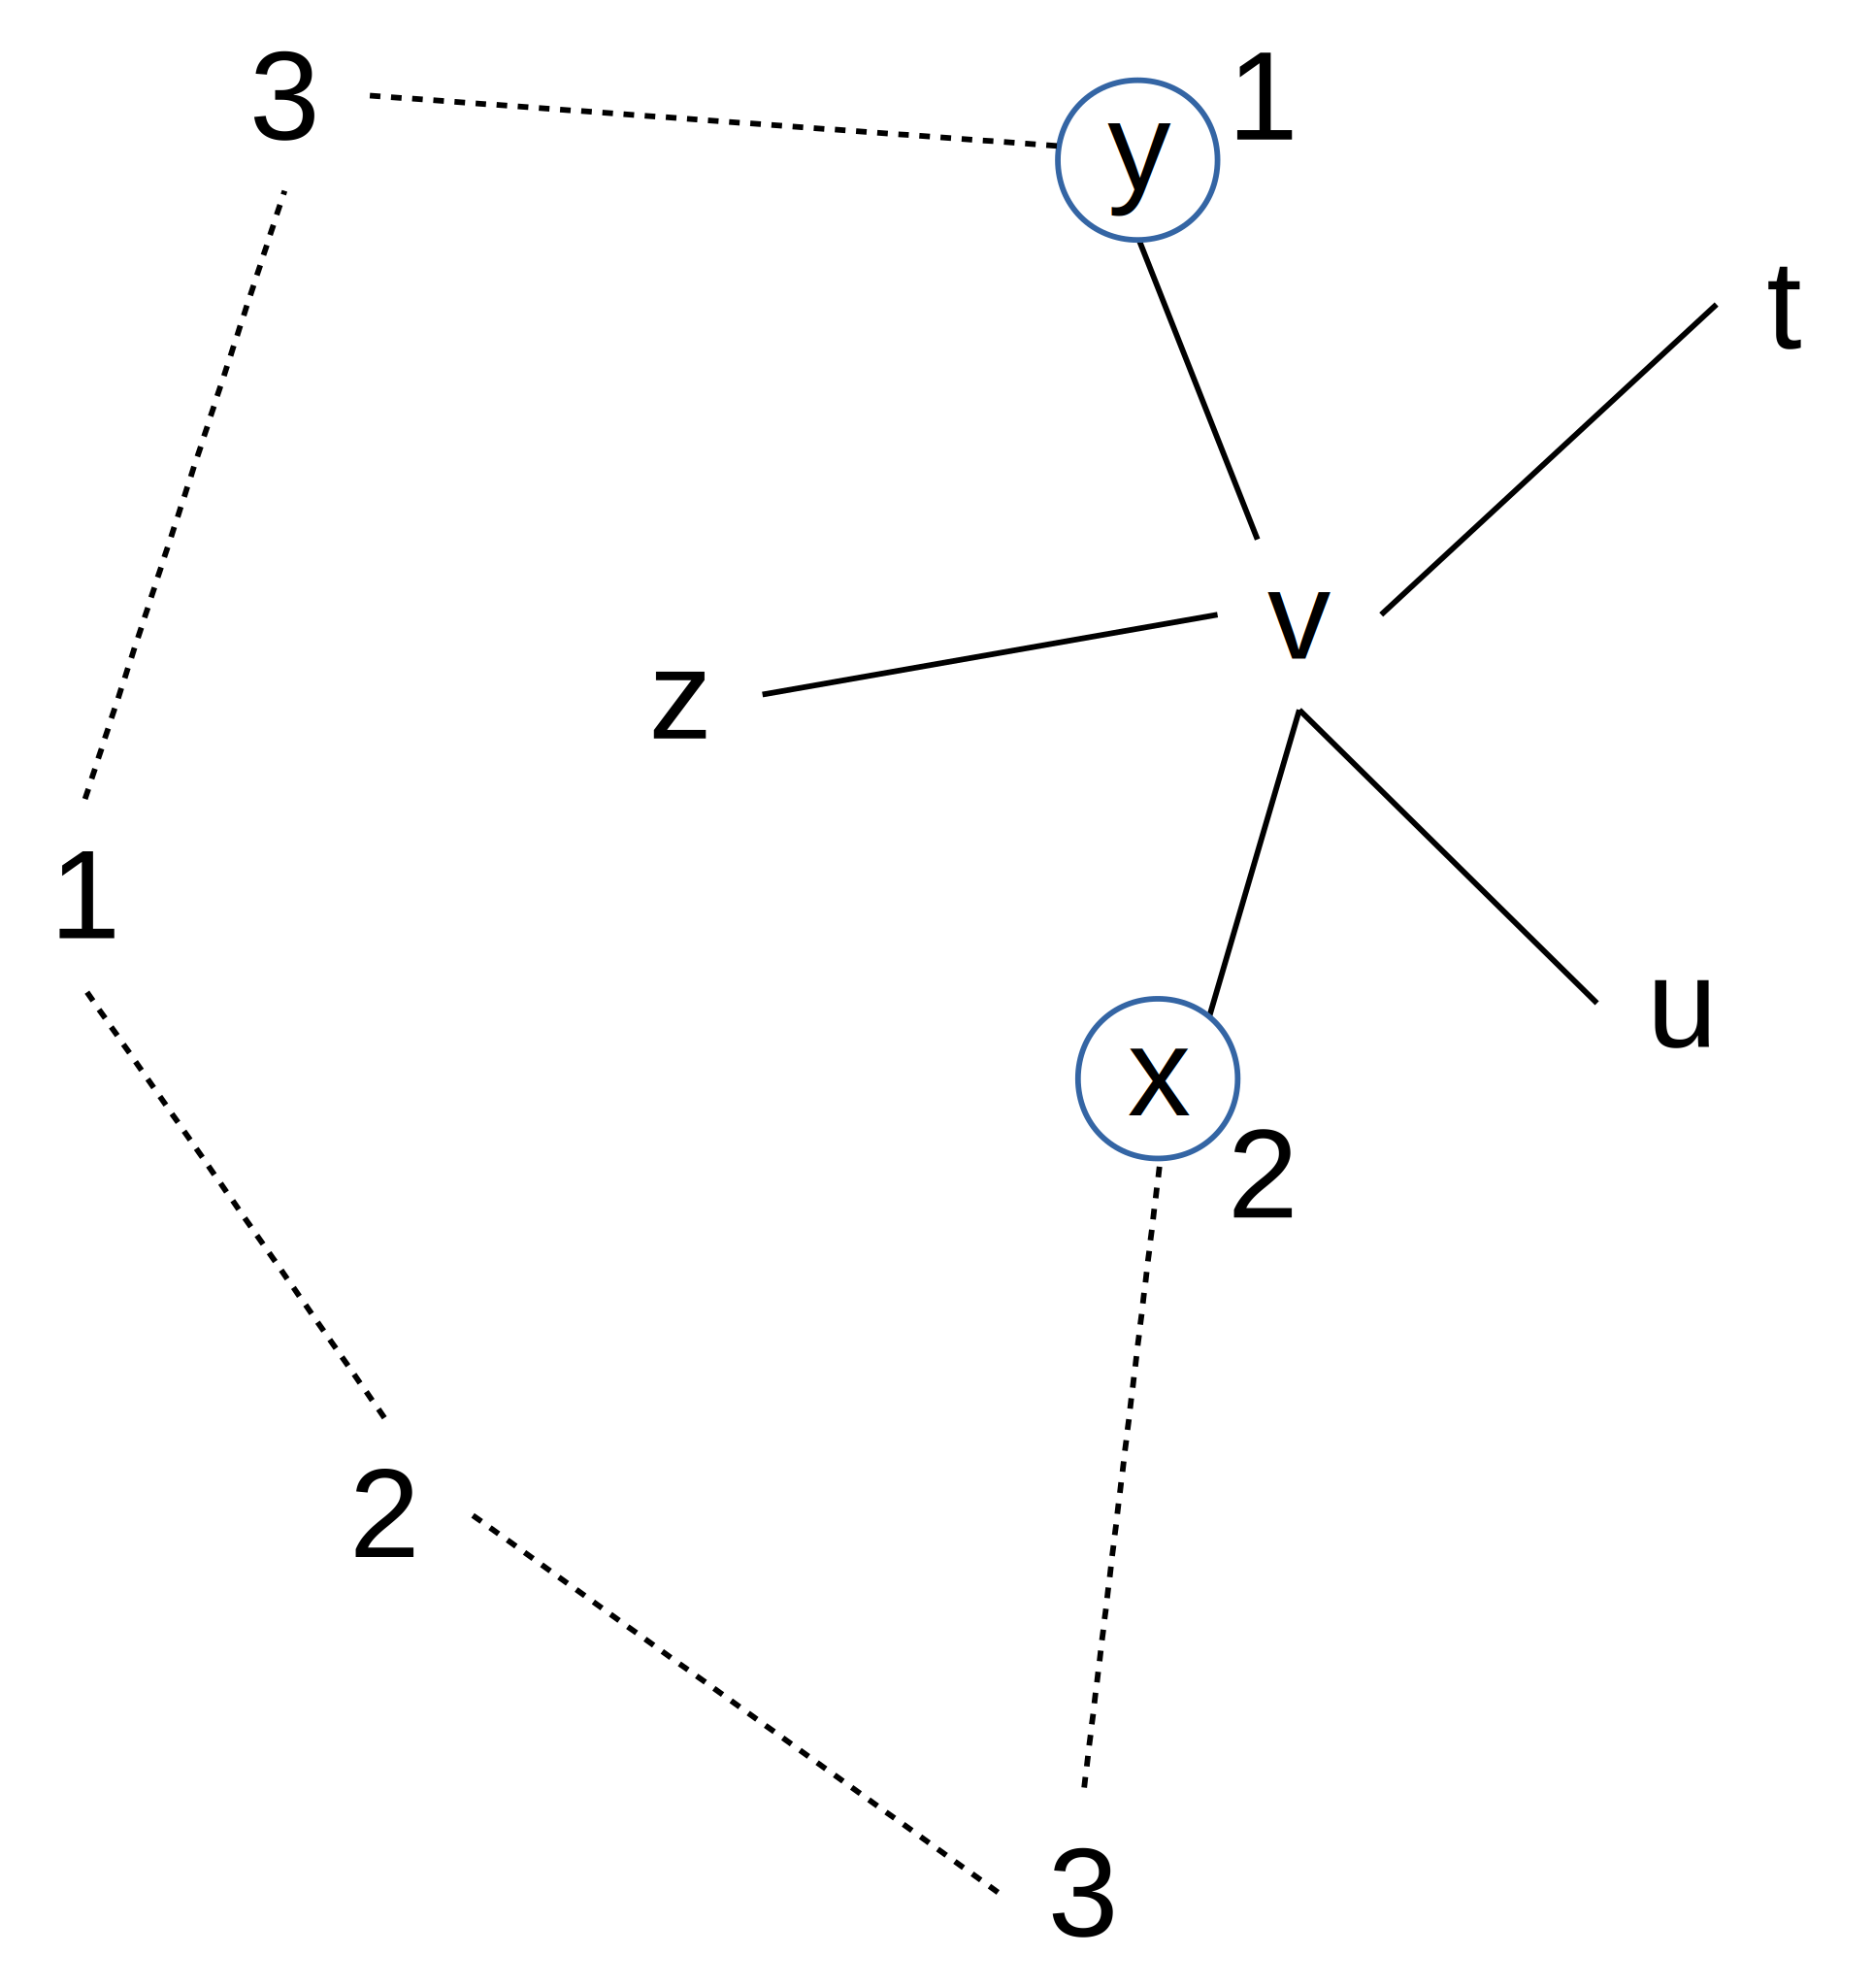
\includegraphics[scale=0.5]{lectures/161125/pix/2.pdf}
                        \begin{itemize}
                            \item betrachte 5-Färbung $\mathcal{C} \colon V(G \setminus \{v\}) \mapsto \{1, \dots, 5\}$, die es nach Rekursion gibt
                            \item betrache $x,y \in V_{xy}$ und sei $V_{xy} \subset V(G)$ die Menge der Knoten mit $\mathcal{C}(x)$- oder $\mathcal{C}(y)$-Färbung
                                \begin{enumerate}
                                    \item es gibt \underline{keinen} Weg von $x \rightsquigarrow y$, der nur Knoten aus $V_{xy}$ nutzt
                                        \begin{itemize}
                                            \item Seien $V'_{xy}$ die $s \in V(G \setminus \{v\})$, die von $x$ nur via $V_{xy}$ erreicht werden
                                            \item Färbe um:
                                            \begin{math}
                                                \mathcal{C'}(s) =
                                                    \begin{cases}
                                                        \mathcal{C}(s) & s \not \in V'_{xy}\\
                                                        \mathcal{C}(y) & s \in V'_{xy}, ~ \mathcal{C}(s) = \mathcal{C}(x)\\
                                                        \mathcal{C}(x) & s \in V'_{xy}, ~ \mathcal{C}(s) = \mathcal{C}(y)
                                                    \end{cases}
                                            \end{math}\\\\
                                            ``Tausche Farben auf $V'_{xy}$'' $\Rightarrow \mathcal{C'}(x) = \mathcal{C'}(y) = \mathcal{C}(y)$
                                        \end{itemize}
                                    \item es gibt einen solchen Pfad $x \rightsquigarrow y$ mit allen Knoten in $V_{xy}$
                                    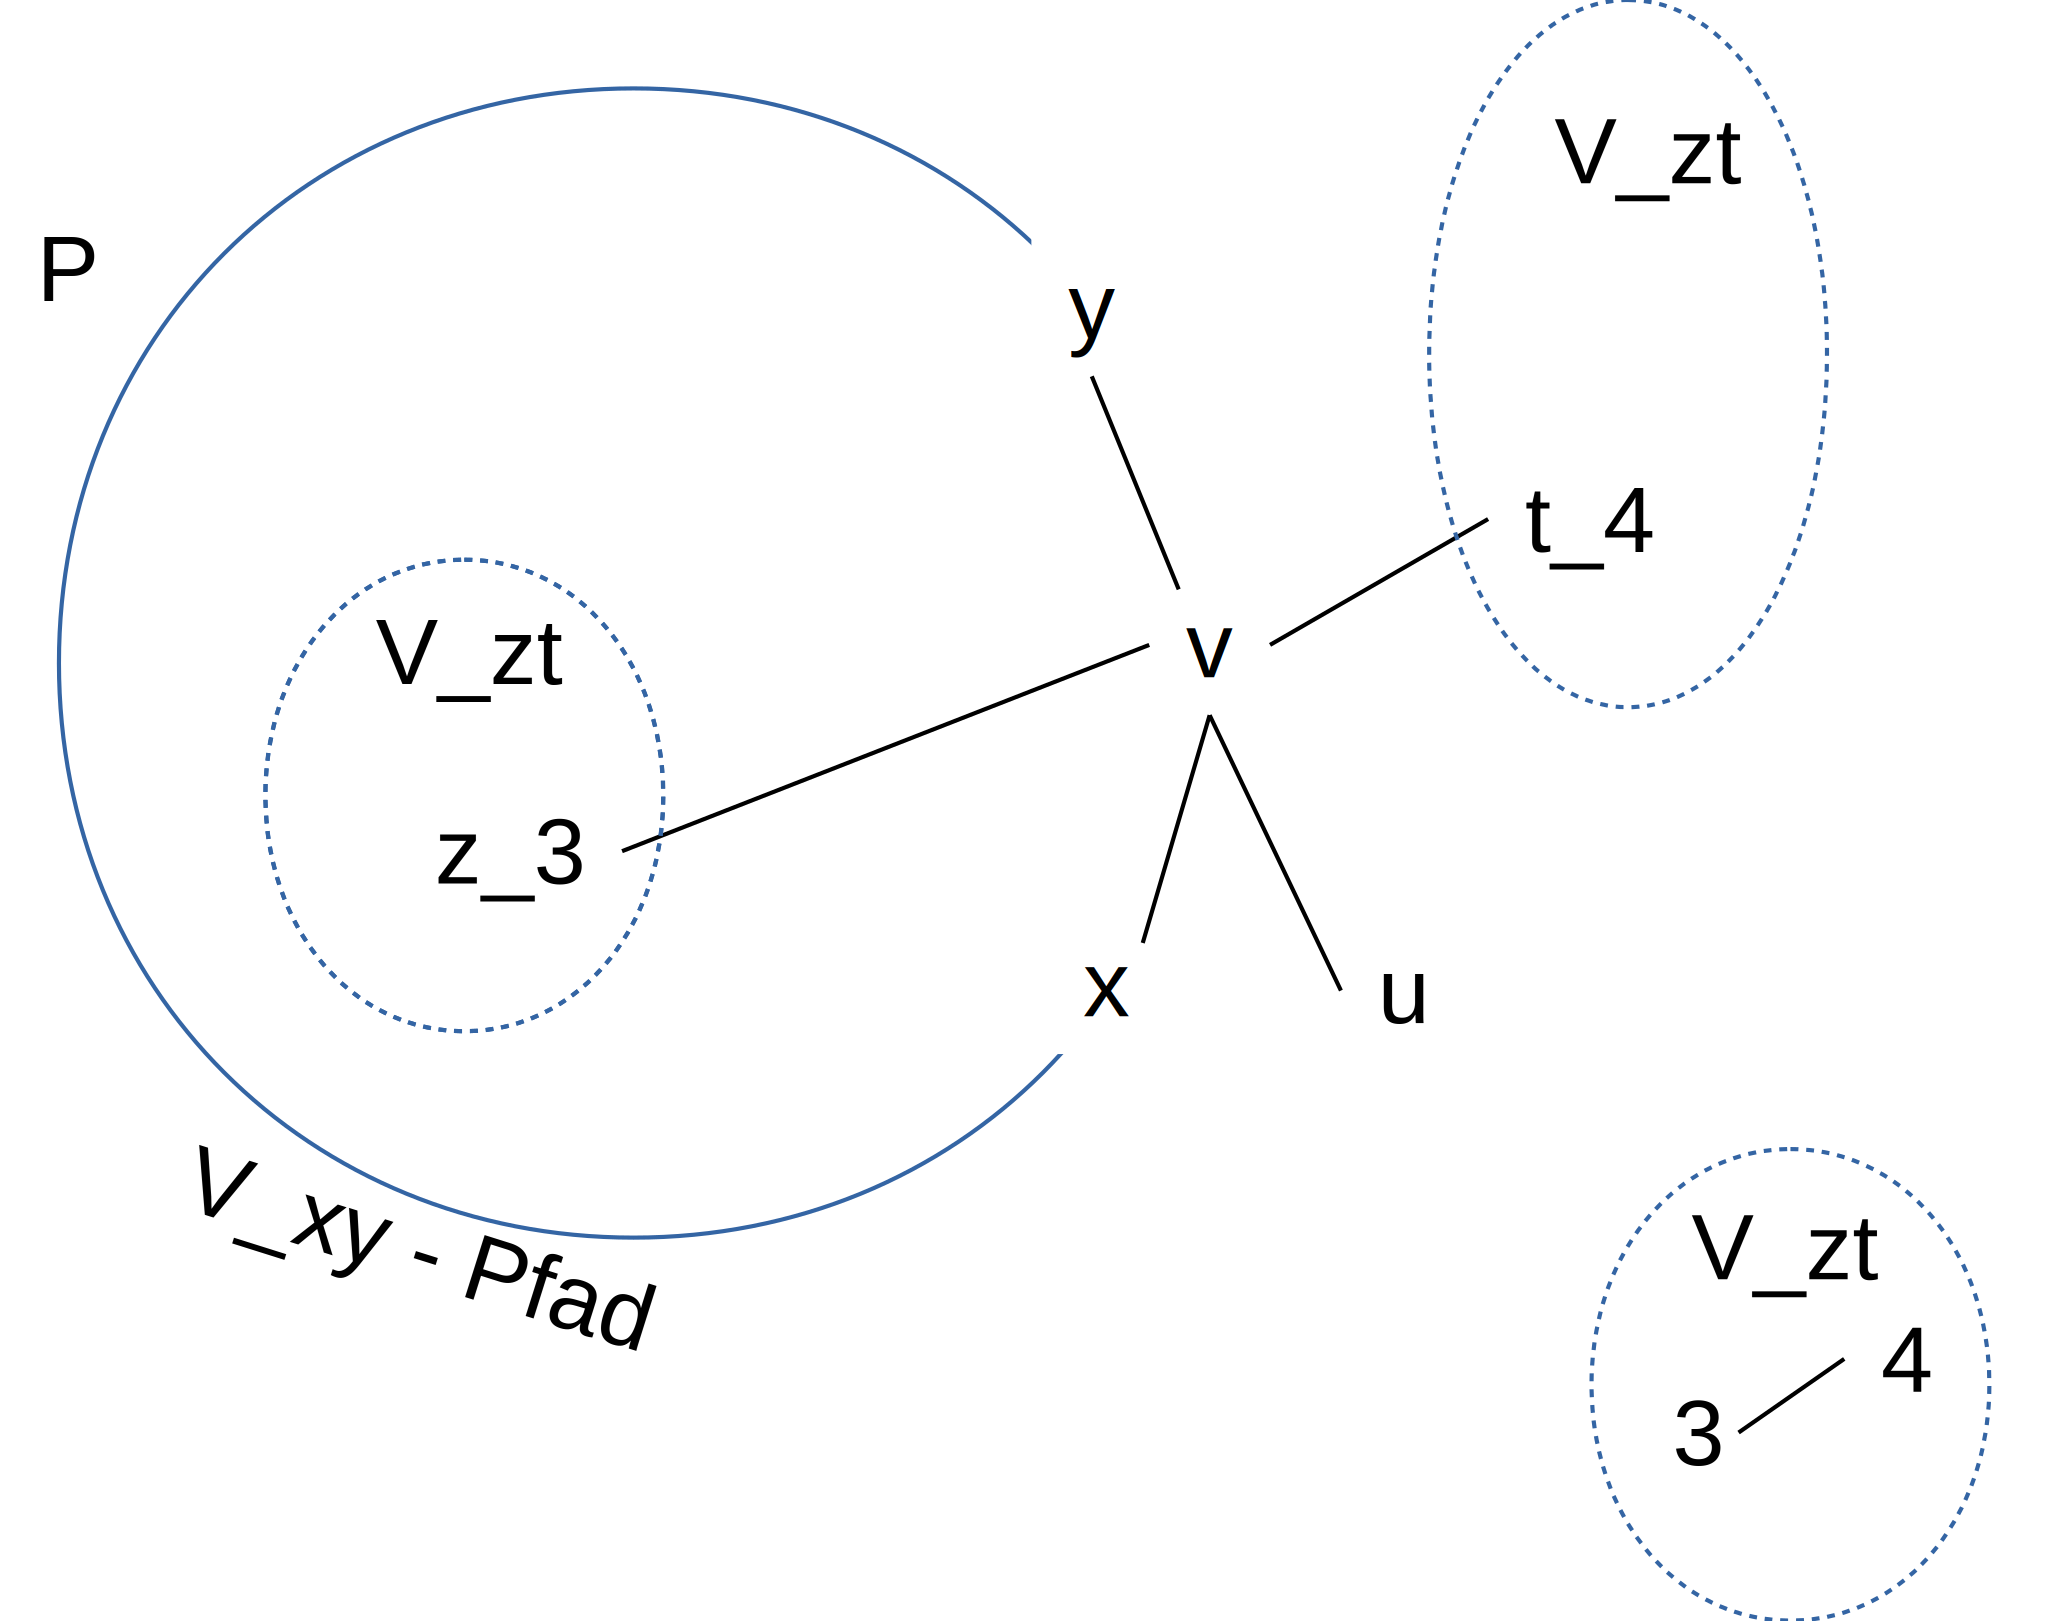
\includegraphics[scale=0.5]{lectures/161125/pix/3.pdf}
                                        \begin{itemize}
                                            \item $V_{zt}$: alle Knoten in $V(G \setminus \{v\})$, die $\mathcal{C}(t)$ oder $\mathcal{C}(z)$ gefärbt sind
                                            \item $V_{xy} \cap V_{zt} = \emptyset$!
                                            \item $V'_{zt}$ kann nur via eines $s \in P$ einen Knoten in $V_{zt} \setminus V'_{zt}$ erreichen
                                        \end{itemize}
                                        Damit lassen sich $z,t$ analog zu Fall (a) färben.
                                \end{enumerate}
                        \end{itemize}
                \end{enumerate}
        \end{description}
    \item[Theorem] Jeder planare Graph ist 4-färbbar
        \begin{description}
            \item[Proof] Es gibt eine Menge von 1936 4-färbbaren Karten, jede nicht Teil eines kleinsten Gegenbeispiels... (Appel, Haken, 1976).
            $\Rightarrow$ Es folgt, dass es kein kleinstes Gegenbeispiel gibt.
        \end{description}
\end{description}

\subsection{Zufallsgraphen}
Sei $G=(V,E)$ mit $V=\{1, \dots, n\}$ fixiert. Wir wollen nun Kanten zufällig auswählen auf dieser fixierten Kantenmenge $\{1, \dots, n\}$, um zufällige Graphen zu generieren. 
Die Menge dieser Zufallsgraphen nennen wir $\mathcal{G}$. \underline{Jede} Kante wird mit Wahrscheinlichkeit $p \in [0, \dots, 1]$ gewählt. 
Sei $G_0$ ein bestimmter Graph. Das Ereignis $\{G_0\}$ mit $G_0$ und m Kanten hat die Wahrscheinlichkeit $p^m \cdot (1-p)^{{n \over 2}-m}$. 
Wahrscheinlichkeitsmaß auf 
$\mathcal{G} ~ \forall e \in [v]^2$\\
$\Omega_e=\{0_e, 1_e\}$\\
$\mathbb{P}(\{1_e\})=p$\\
$\mathbb{P}(\{0_e\})=1-p$\\
$\Omega_\mathcal{G} = \prod\limits_{e \in [v]^2} \Omega_e$

\begin{description}
    \item[Beispiele] Fixiere Graph $H$, $V(H) = V(G)$, ist $H \leqslant G$? \\
        Mit $p^l$, $|E(H)| = l$, $|V(H)| = k$, aber falls $H$ induzierter Teilgraph von $G$ sein soll? \\
         - Nur $p^l (1-p)^{\binom{k}{2} - l}$. \\
        Und was ist mit Subgraph-Isomorphismus?
        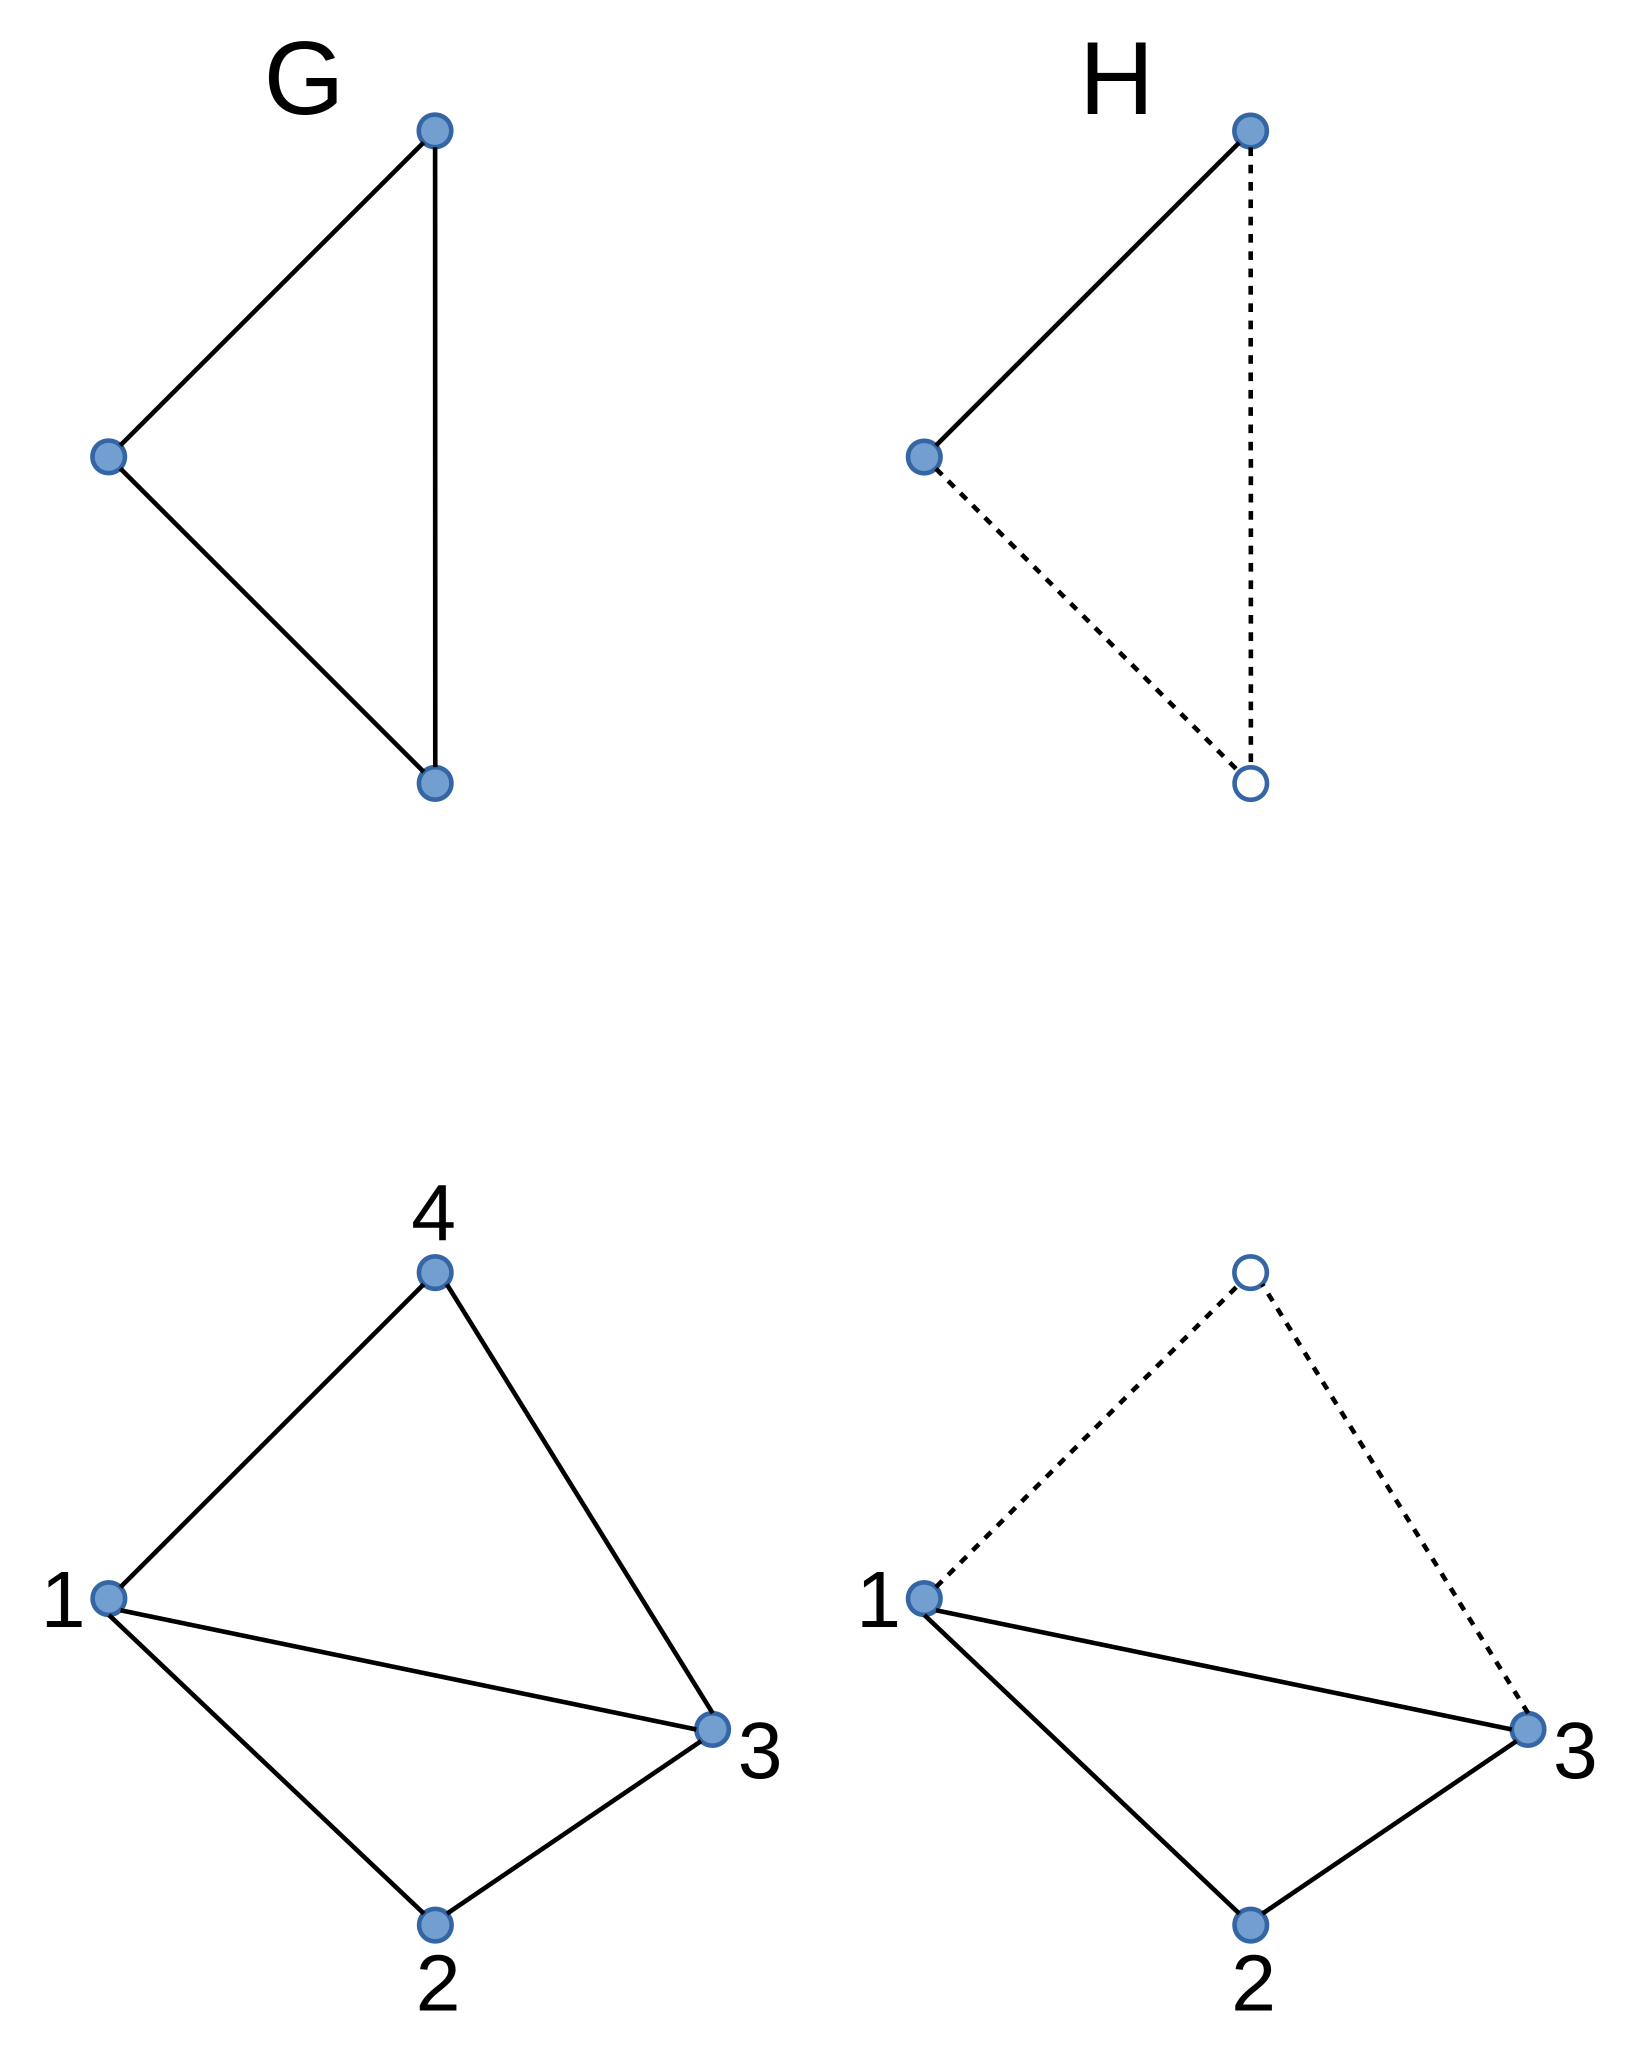
\includegraphics[scale=0.5]{lectures/161125/pix/4.pdf}
        \begin{itemize}
            \item Ereignismengen überlappen
            \item kompliziert
        \end{itemize}
\end{description}

\subsection{Eigenschaften fast aller Graphen}
Falls die Wahrscheinlichkeit, dass $P(G \in \mathcal{G}) \rightarrow 1$ für $n \rightarrow \infty$, dann geschieht $G$ fast sicher.
\begin{description}
    \item[Pro:] Gegeben jedes $H$ als Isomorphie-Klasse, $n \rightarrow \infty$ und $p \in ]0,1[ = (0,1)$, induzierte Kopie von $H$. 
    Dann haben fast alle $G$ in $\mathcal{G}(n,p)$ haben mindestens eine induzierte Kopie von $H$.
    \item[Prf:] Sei $H$ gegeben, $K=V(H)$. Sei $K \leqslant n$. $H$ ist (subgraph-) isomorph zu $G$ mit Wahrscheinlichkeit $r < 0$ ($G$ ist zufällig!). 
        Teile $G$ in $\lfloor {n \over k} \rfloor$ Teilgraphen, um genau so viele ``Versuche'' (für $r > 0$) zu haben. 
        $P(H \not \subseteq G$ induziert) $\leqslant (1-r)^{\lfloor {n \over k} \rfloor} \xrightarrow{n \rightarrow \infty} 0$
\end{description}


\newpage

\section{Vorlesung 25.11.2016}
\subsection{Färbung von Graphen}
\subsubsection{Vertexfärbung}
Zwei durch eine Kante verbundene Knoten haben unterschiedliche Farben.\\
Beispiel wäre eine Landkarte auf der mit so wenig wie möglich Farben die Länder ausgemalt werden, ohne zwei benachbarte Länder gleichfarbig zu haben. Hierbei entspricht jede Facette einen Knoten.\\
\includegraphics[width=0.4\textwidth]{lectures/161125/pix/Vertexfaerbung}
\begin{description}
    \item[Vertexfärbung] Eine Vertexfärbung eines Graphen $G=(V,E)$ ist eine Abbildung $\mathcal{C} \colon V \mapsto \mathcal{S}$, mit $\mathcal{S}=$ Menge der Farben. Es gilt, dass $\mathcal{C}(v) \neq \mathcal{C}(w)$, mit $w,v \in \mathcal{S}$, wenn $v$ und $w$ adjazent ($\{v,w\} \in E$) sind. Die Elemente von $\mathcal{S}$ heißen \emph{Farben}.
    \item[k-Färbung] Ein Graph $G$ ist $k$-färbbar, wenn es für eine Abbildung $\mathcal{C}$ eine Menge $\mathcal{S}=\{1,\dots,k\}$ gibt.
    \item[Chromatische Zahl] Eine chromatische Zahl $\chi(G)$ ist die kleinste natürliche Zahl $k$, sodass G $k$-färbbar ist. $\chi(G) \leqslant \Delta(G) + 1$, mit $\Delta(G) = $ maximaler Grad von $G$
        \begin{description}
            \item[Proof (greedy)] Färbe $v_i$ der Vertices $v_1 \dots v_n$ mit der kleinsten Farbe, die nicht von einem Nachbarn von $v_i$ benutzt wird. Da wir max. $\Delta(G)$ viele Nachbarn für $v_i$ haben, gibt es immer eine freie Farbe.
        \end{description}
        $\chi(G) \geqslant$ Größe der größten Clique
    \item[Lemma] Für jeden einfachen planaren Graphen $G$ ist der Durchschnittsgrad $d(G) < 6$
        \begin{description}
            \item[Proof] $d(G) = 2 \cdot {|E| \over |V|}$ mit $|V| \leqslant 3$, $|E| \leqslant 3  \cdot |V| - 6$, dann $d(G) \leqslant {2(3 \cdot |V|-6) \over |V|} = 6-{12 \over |V|}$
        \end{description}
    \item[Theorem] Jeder simple planare Graph $G$ hat $\chi(G) \leqslant 6$
        \begin{description}
            \item[Proof] Annahme: Jeder simple planare Graph mit $|V| = n$ ist $6$-färbbar.
            \begin{itemize}
                \item Sei $G$ hiermit ein simpler planarer Graph mit $|V| = n+1$
                \item Vom Lemma wissen wir, dass $w \in V$ mit $d(w) \leqslant 5$ existiert
                \item Sei $G' = G \setminus \{w\}$. Via Induktionshypothese ist $G'$ 6-färbbar. Das tun wir dann.
                \item Färbe $w$ mit der (min.) freien Farbe, um $G$ zu färben
            \end{itemize}
        \end{description}
    \item[Theorem] Für jeden simplen planaren Graphen $G$ gilt, dass $\chi(G) \leqslant 5$
        \begin{description}
            \item[Proof] Sei $G=(V,E)$ planar
                \begin{enumerate}
                    \item Falls $|V| \leqslant 5 \rightarrow$ trivial
                    \item Für alle $v \in V(G)$ mit $deg(v) < 5$, färbe $v$ und arbeite mit $G \setminus \{v\}$
                    \item $G$ hat Vertex $v$ mit $deg(v) = 5$
                        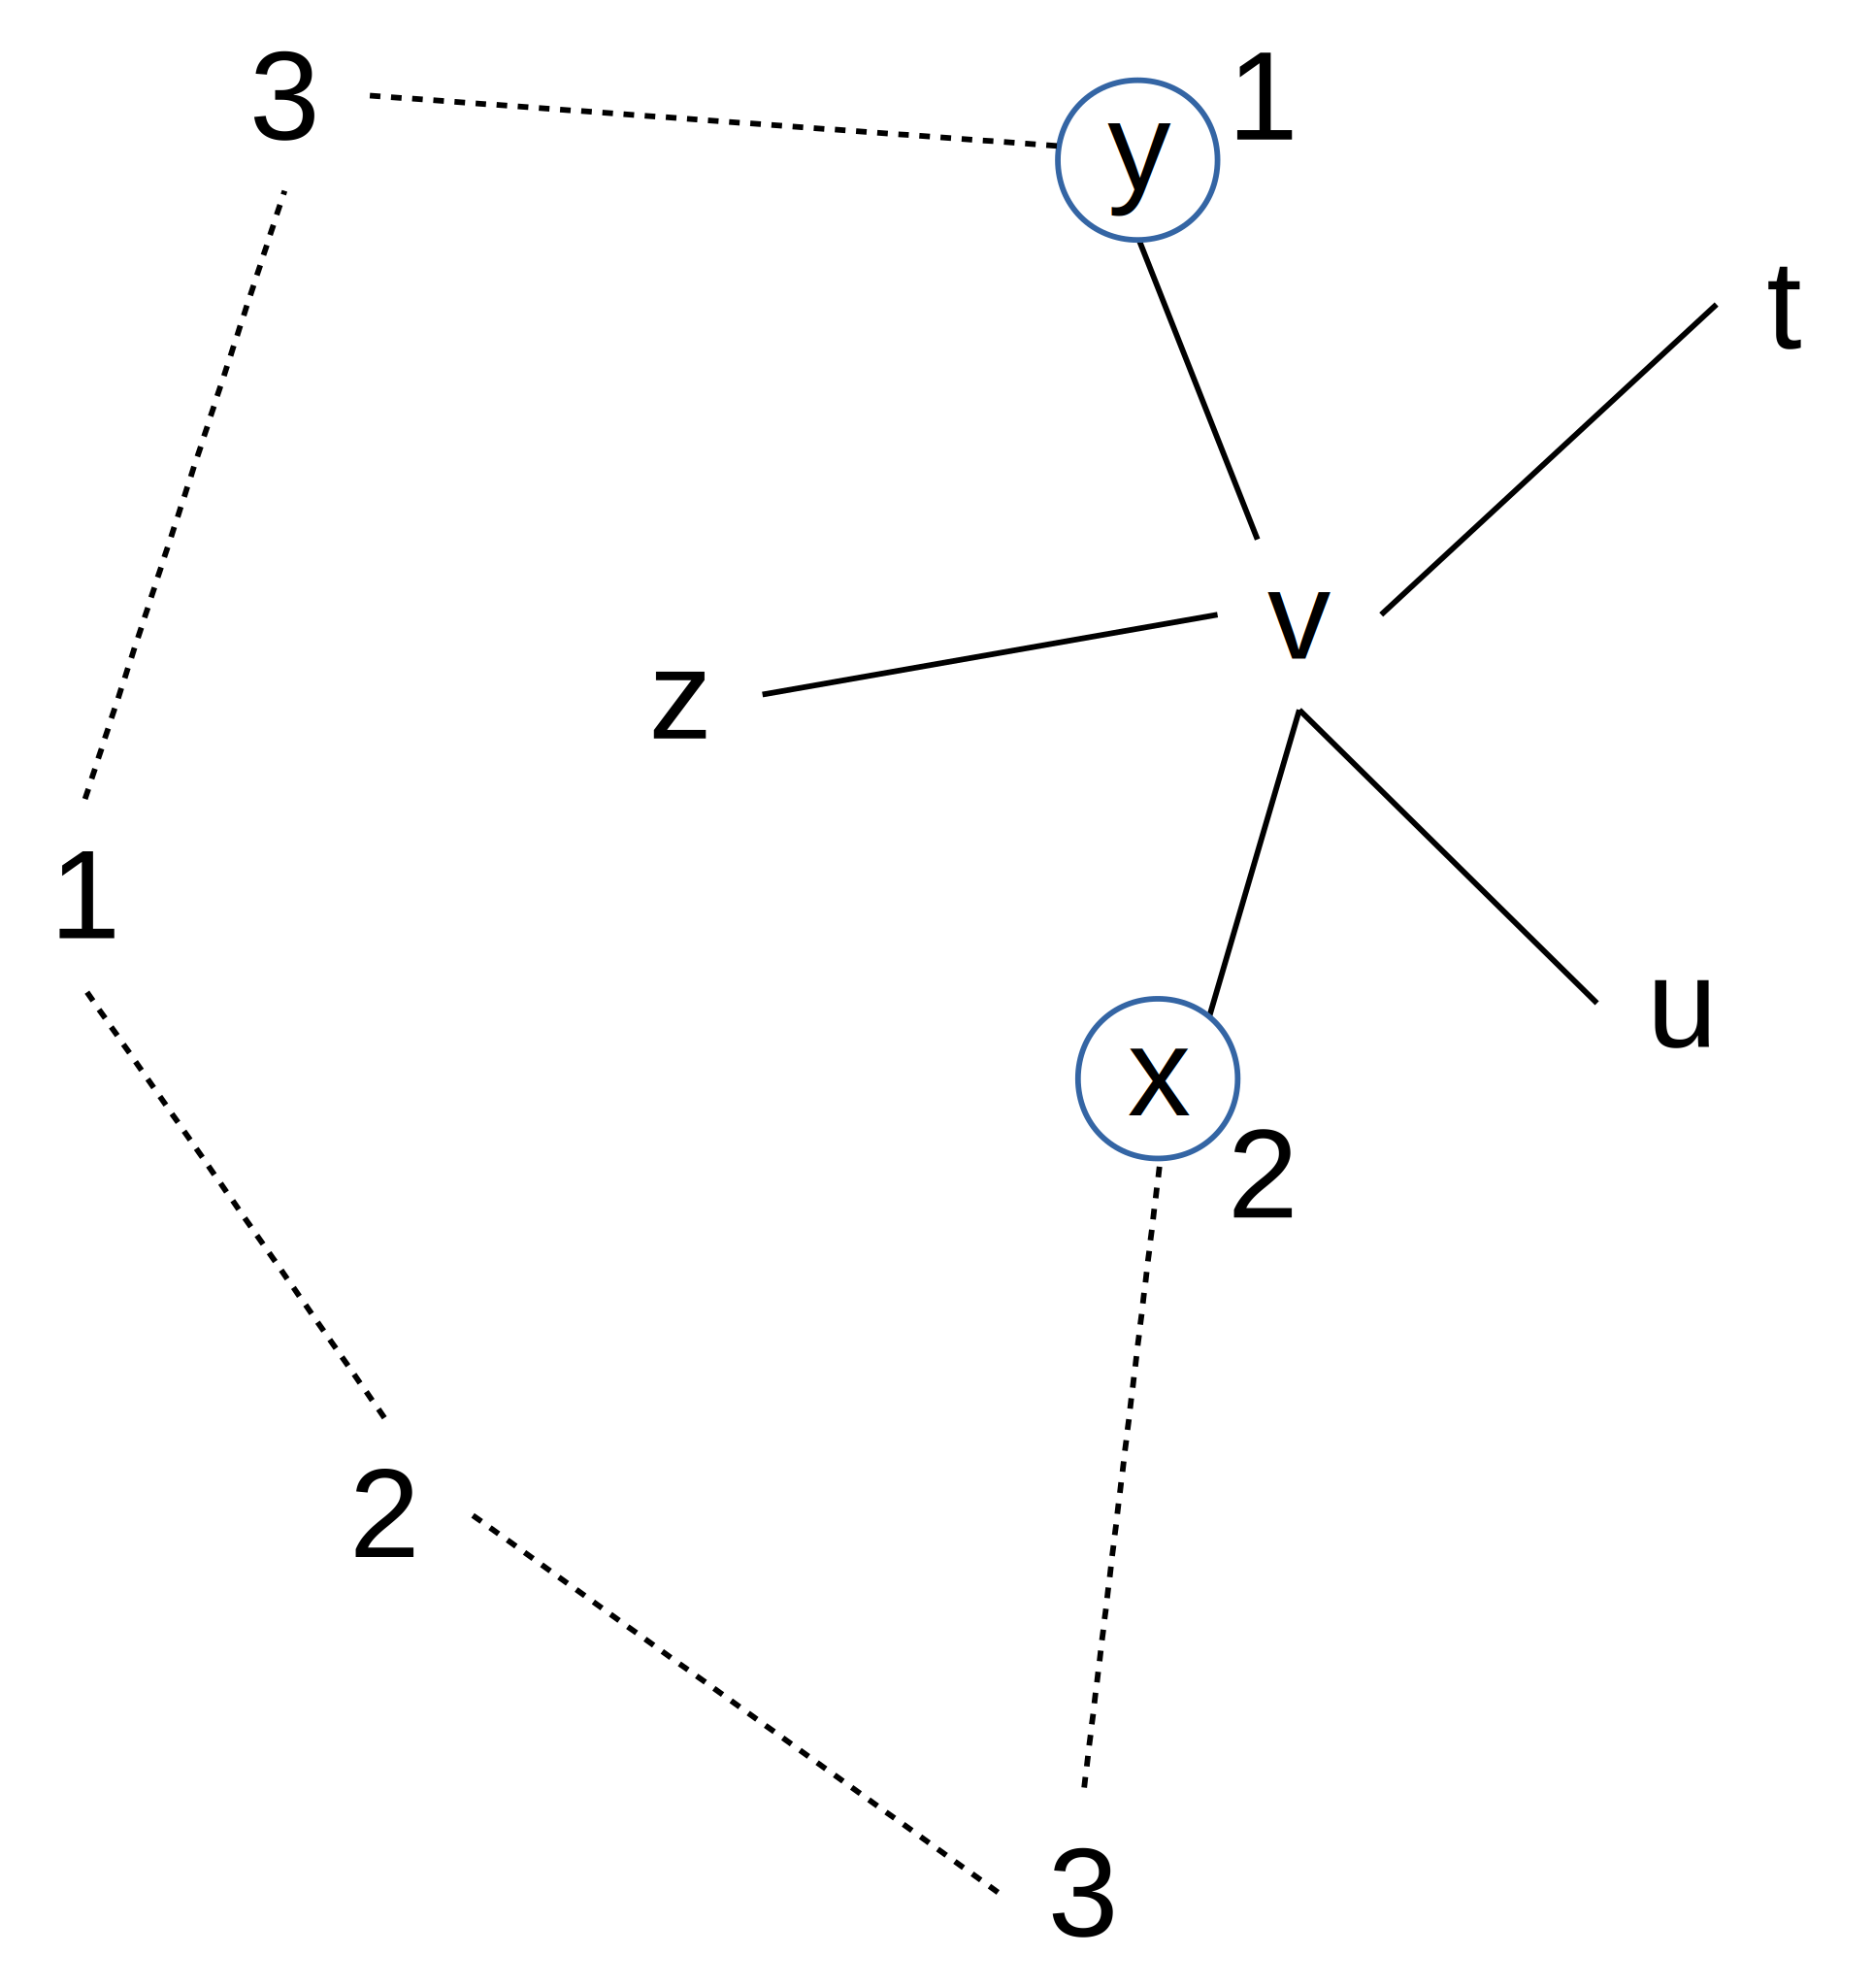
\includegraphics[scale=0.5]{lectures/161125/pix/2.pdf}
                        \begin{itemize}
                            \item betrachte 5-Färbung $\mathcal{C} \colon V(G \setminus \{v\}) \mapsto \{1, \dots, 5\}$, die es nach Rekursion gibt
                            \item betrache $x,y \in V_{xy}$ und sei $V_{xy} \subset V(G)$ die Menge der Knoten mit $\mathcal{C}(x)$- oder $\mathcal{C}(y)$-Färbung
                                \begin{enumerate}
                                    \item es gibt \underline{keinen} Weg von $x \rightsquigarrow y$, der nur Knoten aus $V_{xy}$ nutzt
                                        \begin{itemize}
                                            \item Seien $V'_{xy}$ die $s \in V(G \setminus \{v\})$, die von $x$ nur via $V_{xy}$ erreicht werden
                                            \item Färbe um:
                                            \begin{math}
                                                \mathcal{C'}(s) =
                                                    \begin{cases}
                                                        \mathcal{C}(s) & s \not \in V'_{xy}\\
                                                        \mathcal{C}(y) & s \in V'_{xy}, ~ \mathcal{C}(s) = \mathcal{C}(x)\\
                                                        \mathcal{C}(x) & s \in V'_{xy}, ~ \mathcal{C}(s) = \mathcal{C}(y)
                                                    \end{cases}
                                            \end{math}\\\\
                                            ``Tausche Farben auf $V'_{xy}$'' $\Rightarrow \mathcal{C'}(x) = \mathcal{C'}(y) = \mathcal{C}(y)$
                                        \end{itemize}
                                    \item es gibt einen solchen Pfad $x \rightsquigarrow y$ mit allen Knoten in $V_{xy}$
                                    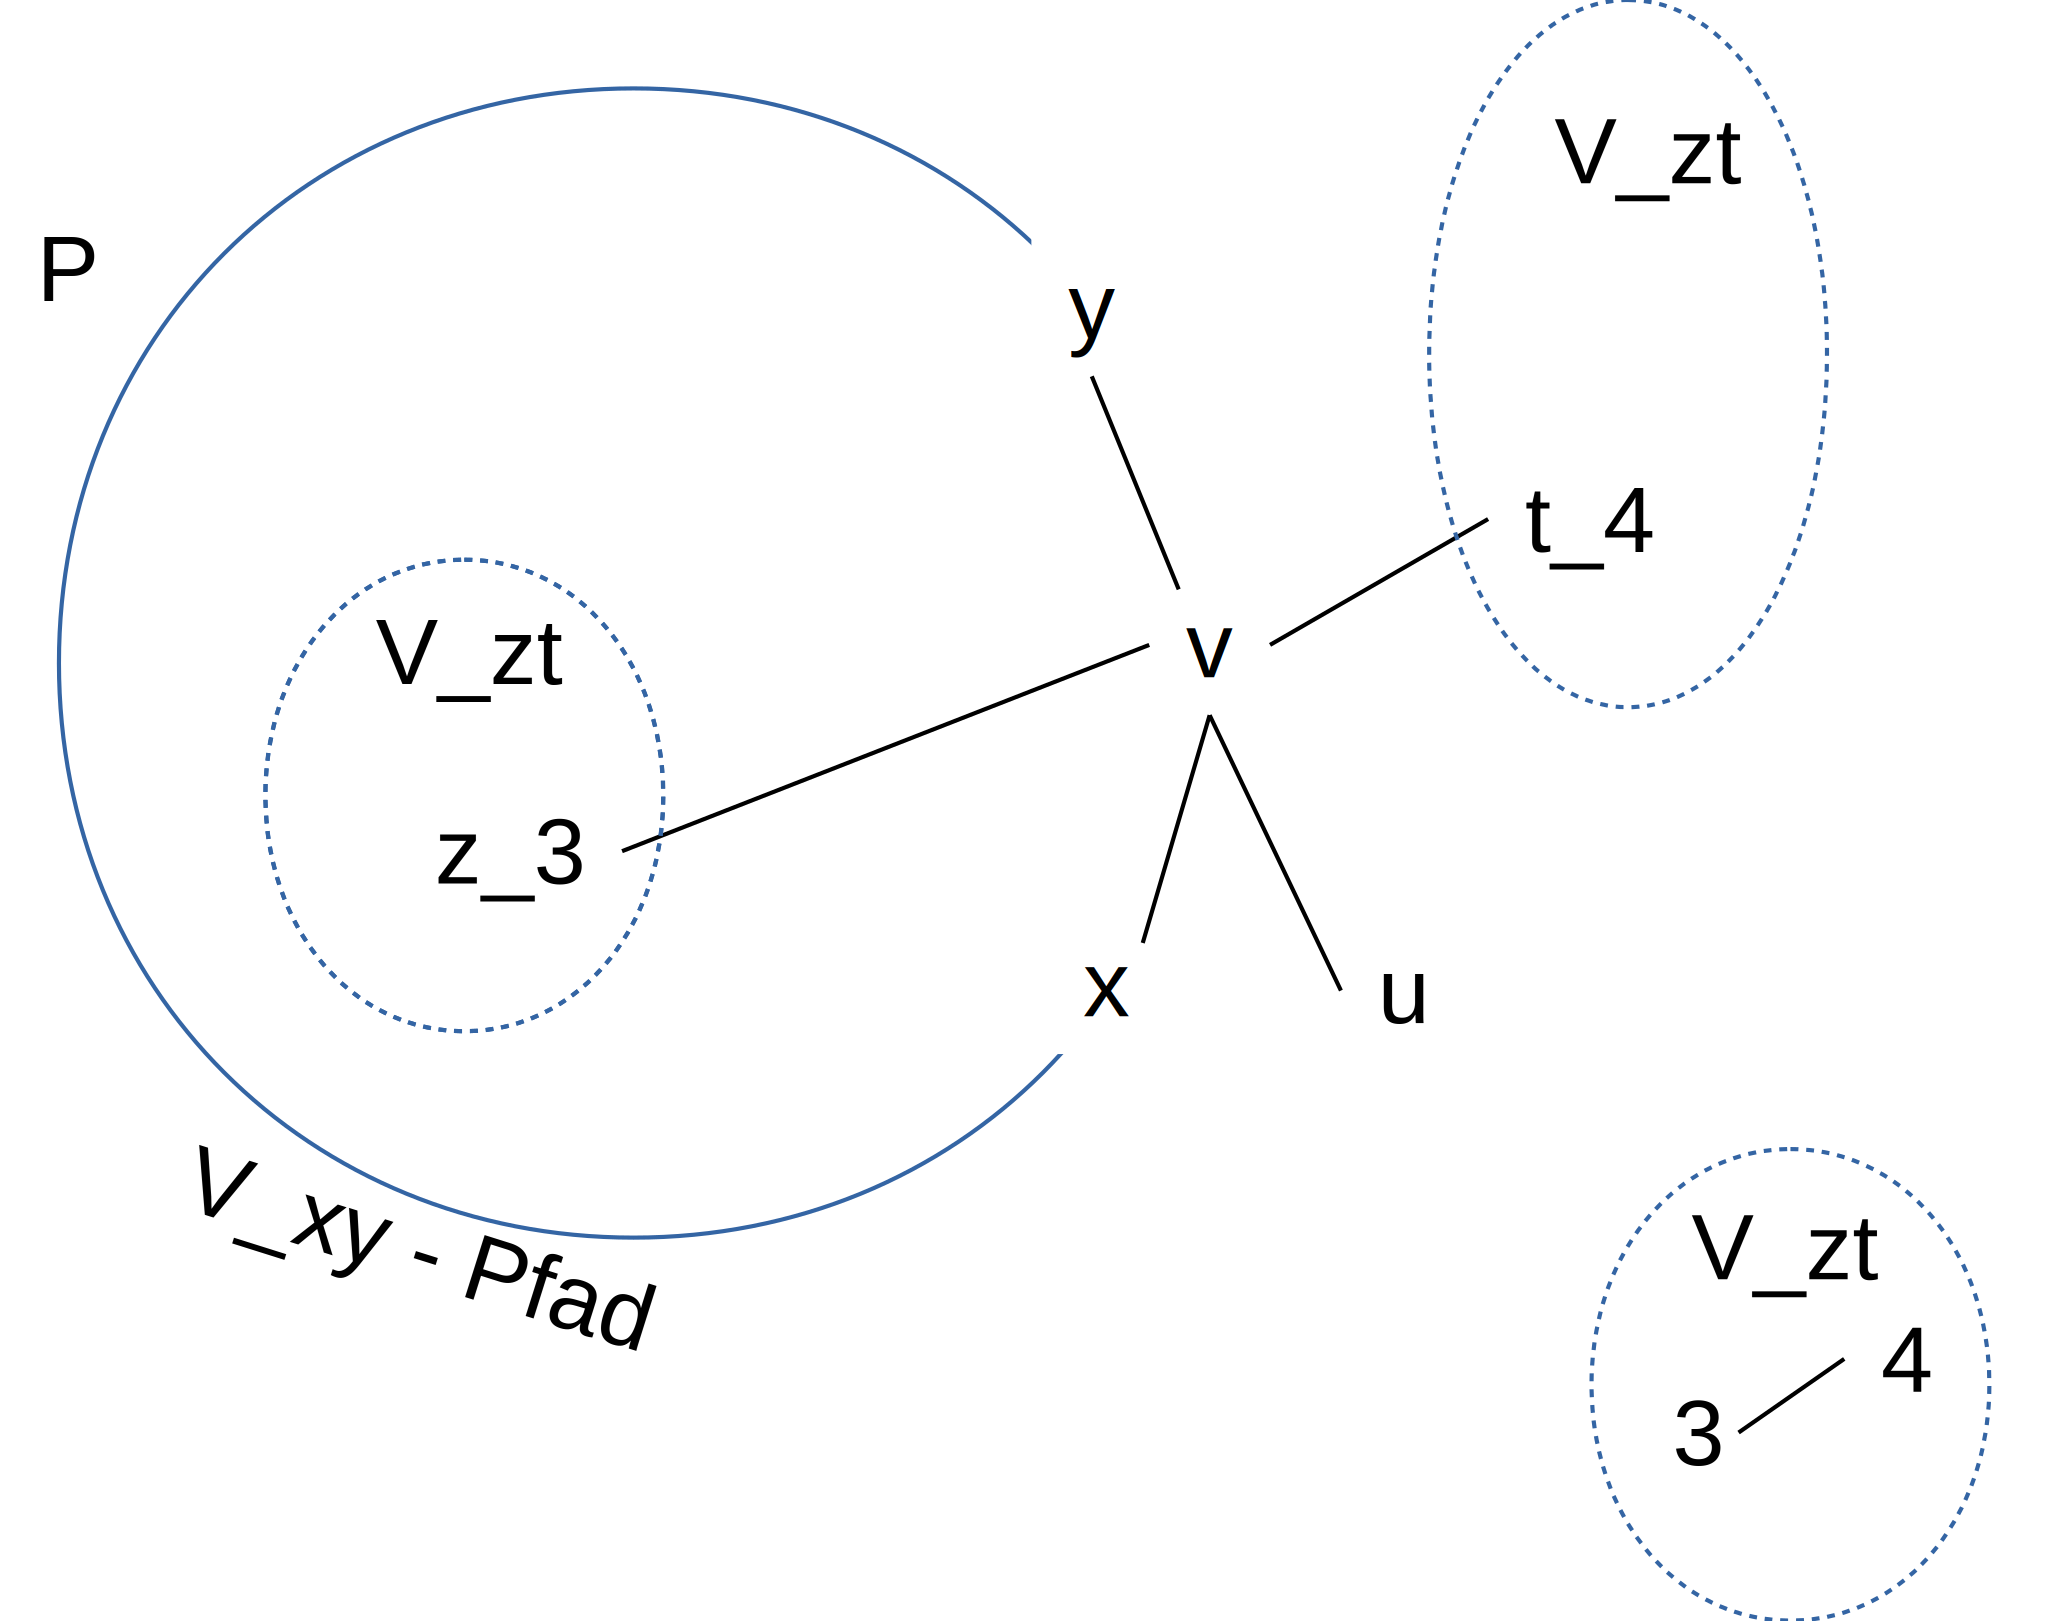
\includegraphics[scale=0.5]{lectures/161125/pix/3.pdf}
                                        \begin{itemize}
                                            \item $V_{zt}$: alle Knoten in $V(G \setminus \{v\})$, die $\mathcal{C}(t)$ oder $\mathcal{C}(z)$ gefärbt sind
                                            \item $V_{xy} \cap V_{zt} = \emptyset$!
                                            \item $V'_{zt}$ kann nur via eines $s \in P$ einen Knoten in $V_{zt} \setminus V'_{zt}$ erreichen
                                        \end{itemize}
                                        Damit lassen sich $z,t$ analog zu Fall (a) färben.
                                \end{enumerate}
                        \end{itemize}
                \end{enumerate}
        \end{description}
    \item[Theorem] Jeder planare Graph ist 4-färbbar
        \begin{description}
            \item[Proof] Es gibt eine Menge von 1936 4-färbbaren Karten, jede nicht Teil eines kleinsten Gegenbeispiels... (Appel, Haken, 1976).
            $\Rightarrow$ Es folgt, dass es kein kleinstes Gegenbeispiel gibt.
        \end{description}
\end{description}

\subsection{Zufallsgraphen}
Sei $G=(V,E)$ mit $V=\{1, \dots, n\}$ fixiert. Wir wollen nun Kanten zufällig auswählen auf dieser fixierten Kantenmenge $\{1, \dots, n\}$, um zufällige Graphen zu generieren. 
Die Menge dieser Zufallsgraphen nennen wir $\mathcal{G}$. \underline{Jede} Kante wird mit Wahrscheinlichkeit $p \in [0, \dots, 1]$ gewählt. 
Sei $G_0$ ein bestimmter Graph. Das Ereignis $\{G_0\}$ mit $G_0$ und m Kanten hat die Wahrscheinlichkeit $p^m \cdot (1-p)^{{n \over 2}-m}$. 
Wahrscheinlichkeitsmaß auf 
$\mathcal{G} ~ \forall e \in [v]^2$\\
$\Omega_e=\{0_e, 1_e\}$\\
$\mathbb{P}(\{1_e\})=p$\\
$\mathbb{P}(\{0_e\})=1-p$\\
$\Omega_\mathcal{G} = \prod\limits_{e \in [v]^2} \Omega_e$

\begin{description}
    \item[Beispiele] Fixiere Graph $H$, $V(H) = V(G)$, ist $H \leqslant G$? \\
        Mit $p^l$, $|E(H)| = l$, $|V(H)| = k$, aber falls $H$ induzierter Teilgraph von $G$ sein soll? \\
         - Nur $p^l (1-p)^{\binom{k}{2} - l}$. \\
        Und was ist mit Subgraph-Isomorphismus?
        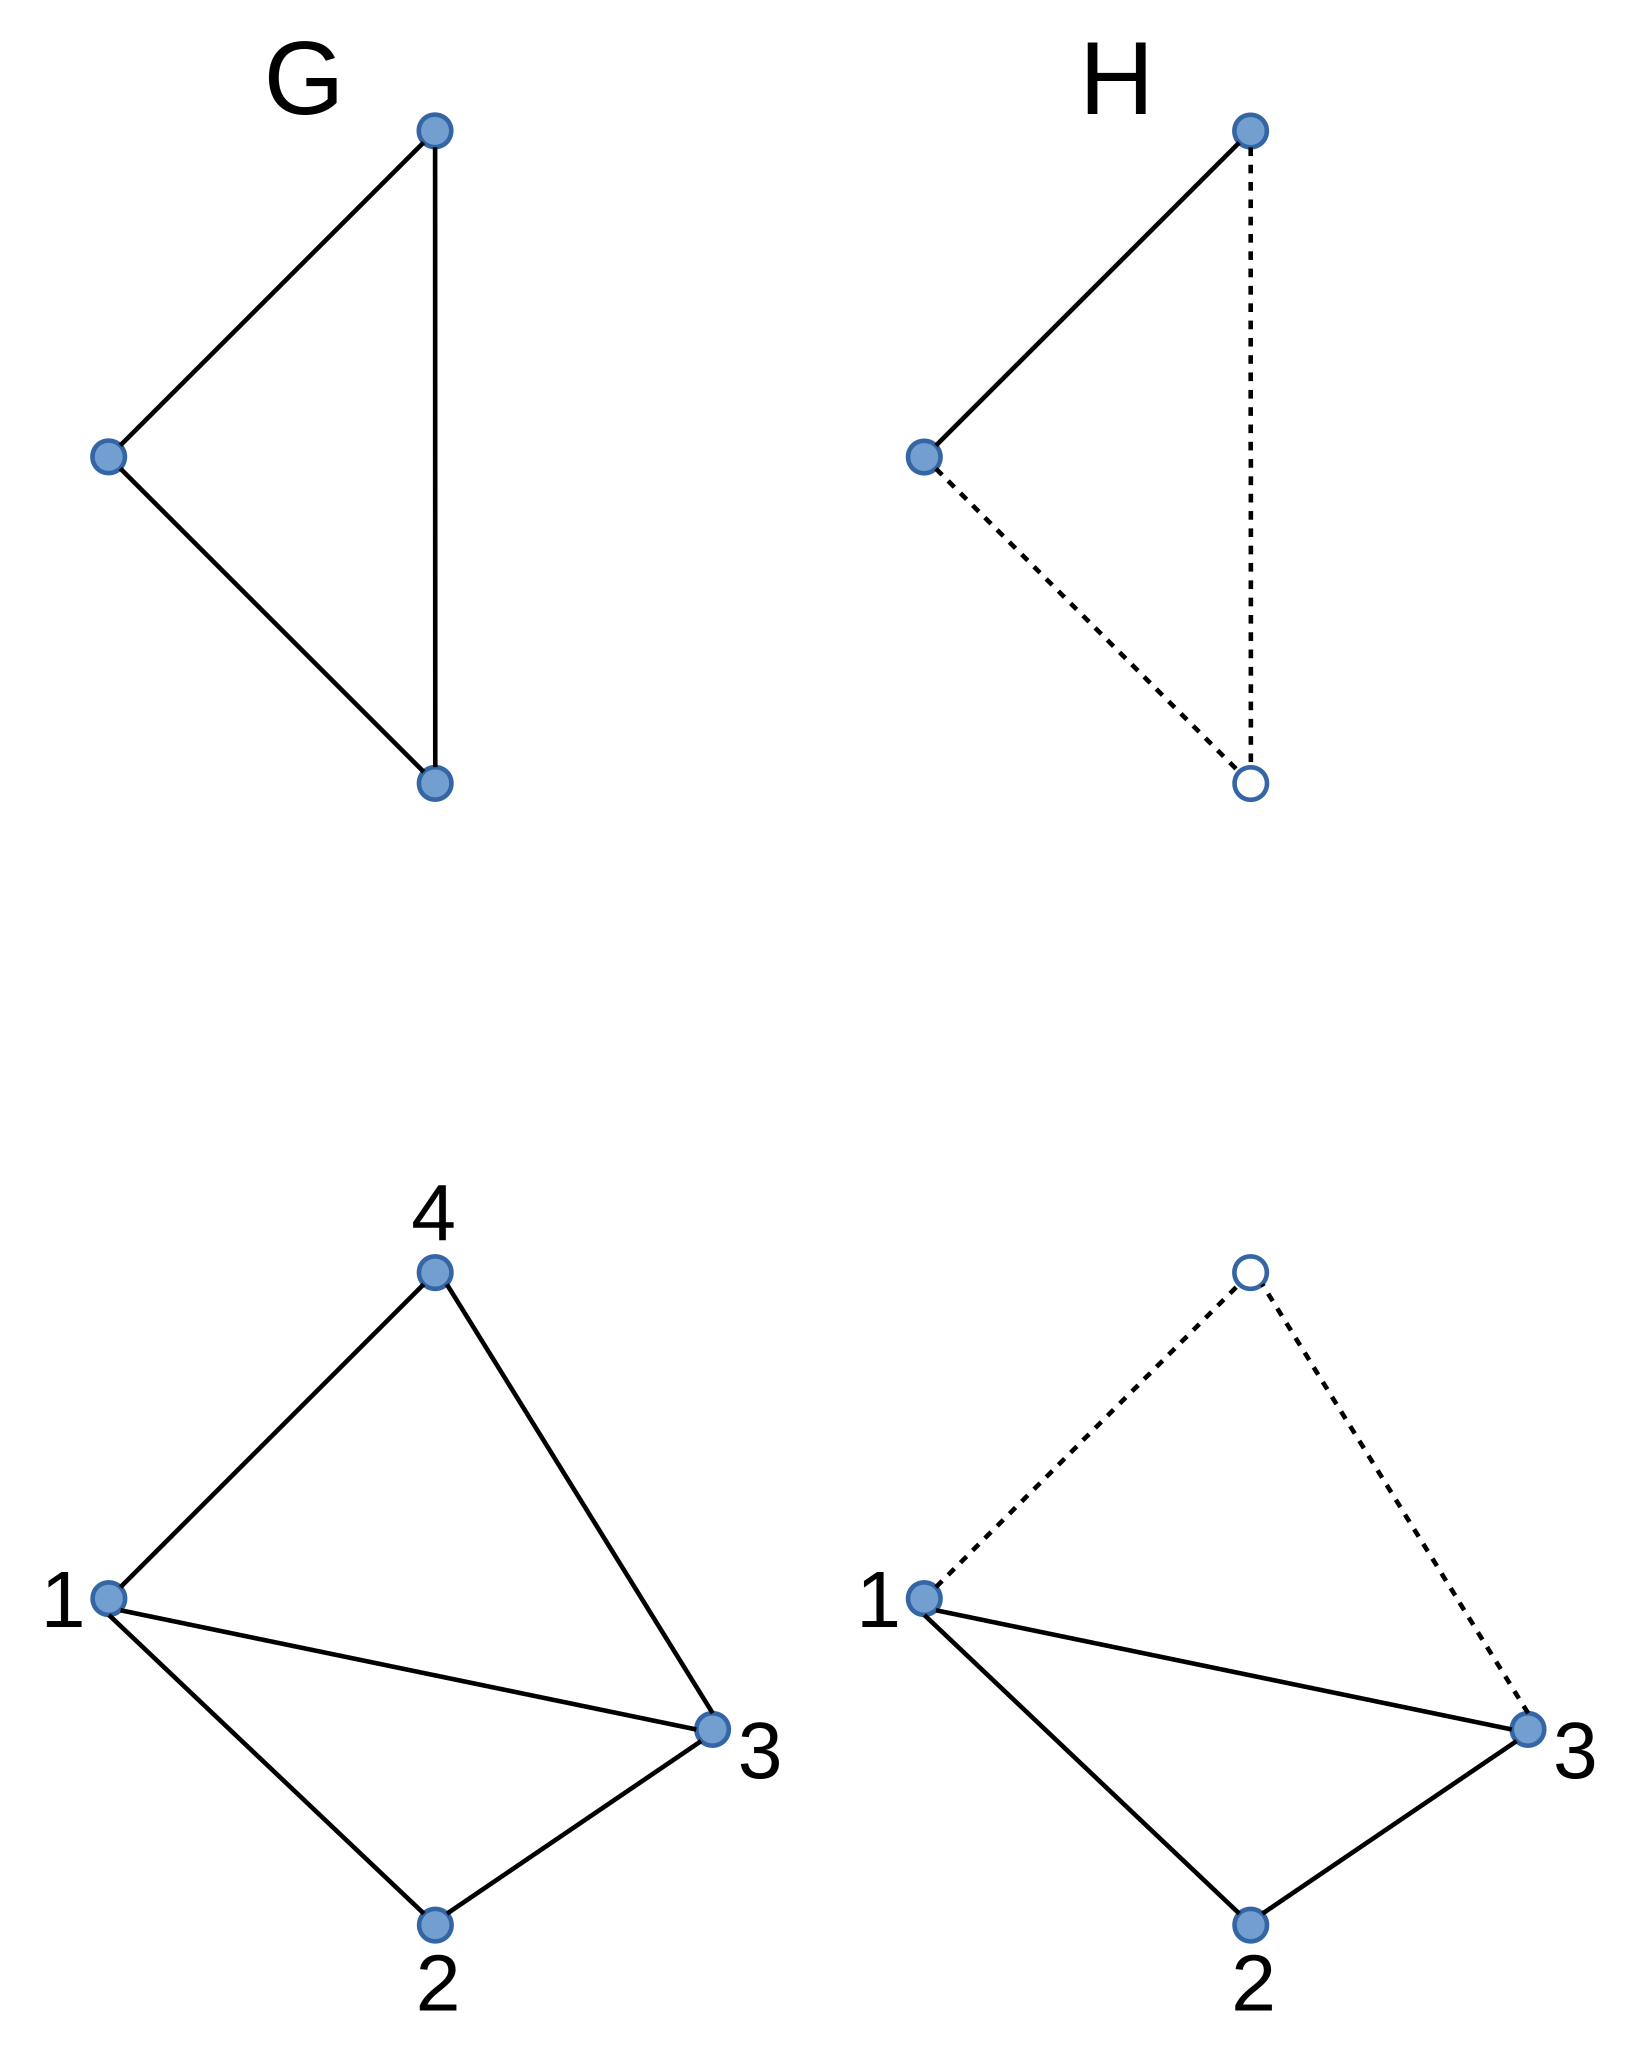
\includegraphics[scale=0.5]{lectures/161125/pix/4.pdf}
        \begin{itemize}
            \item Ereignismengen überlappen
            \item kompliziert
        \end{itemize}
\end{description}

\subsection{Eigenschaften fast aller Graphen}
Falls die Wahrscheinlichkeit, dass $P(G \in \mathcal{G}) \rightarrow 1$ für $n \rightarrow \infty$, dann geschieht $G$ fast sicher.
\begin{description}
    \item[Pro:] Gegeben jedes $H$ als Isomorphie-Klasse, $n \rightarrow \infty$ und $p \in ]0,1[ = (0,1)$, induzierte Kopie von $H$. 
    Dann haben fast alle $G$ in $\mathcal{G}(n,p)$ haben mindestens eine induzierte Kopie von $H$.
    \item[Prf:] Sei $H$ gegeben, $K=V(H)$. Sei $K \leqslant n$. $H$ ist (subgraph-) isomorph zu $G$ mit Wahrscheinlichkeit $r < 0$ ($G$ ist zufällig!). 
        Teile $G$ in $\lfloor {n \over k} \rfloor$ Teilgraphen, um genau so viele ``Versuche'' (für $r > 0$) zu haben. 
        $P(H \not \subseteq G$ induziert) $\leqslant (1-r)^{\lfloor {n \over k} \rfloor} \xrightarrow{n \rightarrow \infty} 0$
\end{description}


\newpage

\section{Vorlesung 25.11.2016}
\subsection{Färbung von Graphen}
\subsubsection{Vertexfärbung}
Zwei durch eine Kante verbundene Knoten haben unterschiedliche Farben.\\
Beispiel wäre eine Landkarte auf der mit so wenig wie möglich Farben die Länder ausgemalt werden, ohne zwei benachbarte Länder gleichfarbig zu haben. Hierbei entspricht jede Facette einen Knoten.\\
\includegraphics[width=0.4\textwidth]{lectures/161125/pix/Vertexfaerbung}
\begin{description}
    \item[Vertexfärbung] Eine Vertexfärbung eines Graphen $G=(V,E)$ ist eine Abbildung $\mathcal{C} \colon V \mapsto \mathcal{S}$, mit $\mathcal{S}=$ Menge der Farben. Es gilt, dass $\mathcal{C}(v) \neq \mathcal{C}(w)$, mit $w,v \in \mathcal{S}$, wenn $v$ und $w$ adjazent ($\{v,w\} \in E$) sind. Die Elemente von $\mathcal{S}$ heißen \emph{Farben}.
    \item[k-Färbung] Ein Graph $G$ ist $k$-färbbar, wenn es für eine Abbildung $\mathcal{C}$ eine Menge $\mathcal{S}=\{1,\dots,k\}$ gibt.
    \item[Chromatische Zahl] Eine chromatische Zahl $\chi(G)$ ist die kleinste natürliche Zahl $k$, sodass G $k$-färbbar ist. $\chi(G) \leqslant \Delta(G) + 1$, mit $\Delta(G) = $ maximaler Grad von $G$
        \begin{description}
            \item[Proof (greedy)] Färbe $v_i$ der Vertices $v_1 \dots v_n$ mit der kleinsten Farbe, die nicht von einem Nachbarn von $v_i$ benutzt wird. Da wir max. $\Delta(G)$ viele Nachbarn für $v_i$ haben, gibt es immer eine freie Farbe.
        \end{description}
        $\chi(G) \geqslant$ Größe der größten Clique
    \item[Lemma] Für jeden einfachen planaren Graphen $G$ ist der Durchschnittsgrad $d(G) < 6$
        \begin{description}
            \item[Proof] $d(G) = 2 \cdot {|E| \over |V|}$ mit $|V| \leqslant 3$, $|E| \leqslant 3  \cdot |V| - 6$, dann $d(G) \leqslant {2(3 \cdot |V|-6) \over |V|} = 6-{12 \over |V|}$
        \end{description}
    \item[Theorem] Jeder simple planare Graph $G$ hat $\chi(G) \leqslant 6$
        \begin{description}
            \item[Proof] Annahme: Jeder simple planare Graph mit $|V| = n$ ist $6$-färbbar.
            \begin{itemize}
                \item Sei $G$ hiermit ein simpler planarer Graph mit $|V| = n+1$
                \item Vom Lemma wissen wir, dass $w \in V$ mit $d(w) \leqslant 5$ existiert
                \item Sei $G' = G \setminus \{w\}$. Via Induktionshypothese ist $G'$ 6-färbbar. Das tun wir dann.
                \item Färbe $w$ mit der (min.) freien Farbe, um $G$ zu färben
            \end{itemize}
        \end{description}
    \item[Theorem] Für jeden simplen planaren Graphen $G$ gilt, dass $\chi(G) \leqslant 5$
        \begin{description}
            \item[Proof] Sei $G=(V,E)$ planar
                \begin{enumerate}
                    \item Falls $|V| \leqslant 5 \rightarrow$ trivial
                    \item Für alle $v \in V(G)$ mit $deg(v) < 5$, färbe $v$ und arbeite mit $G \setminus \{v\}$
                    \item $G$ hat Vertex $v$ mit $deg(v) = 5$
                        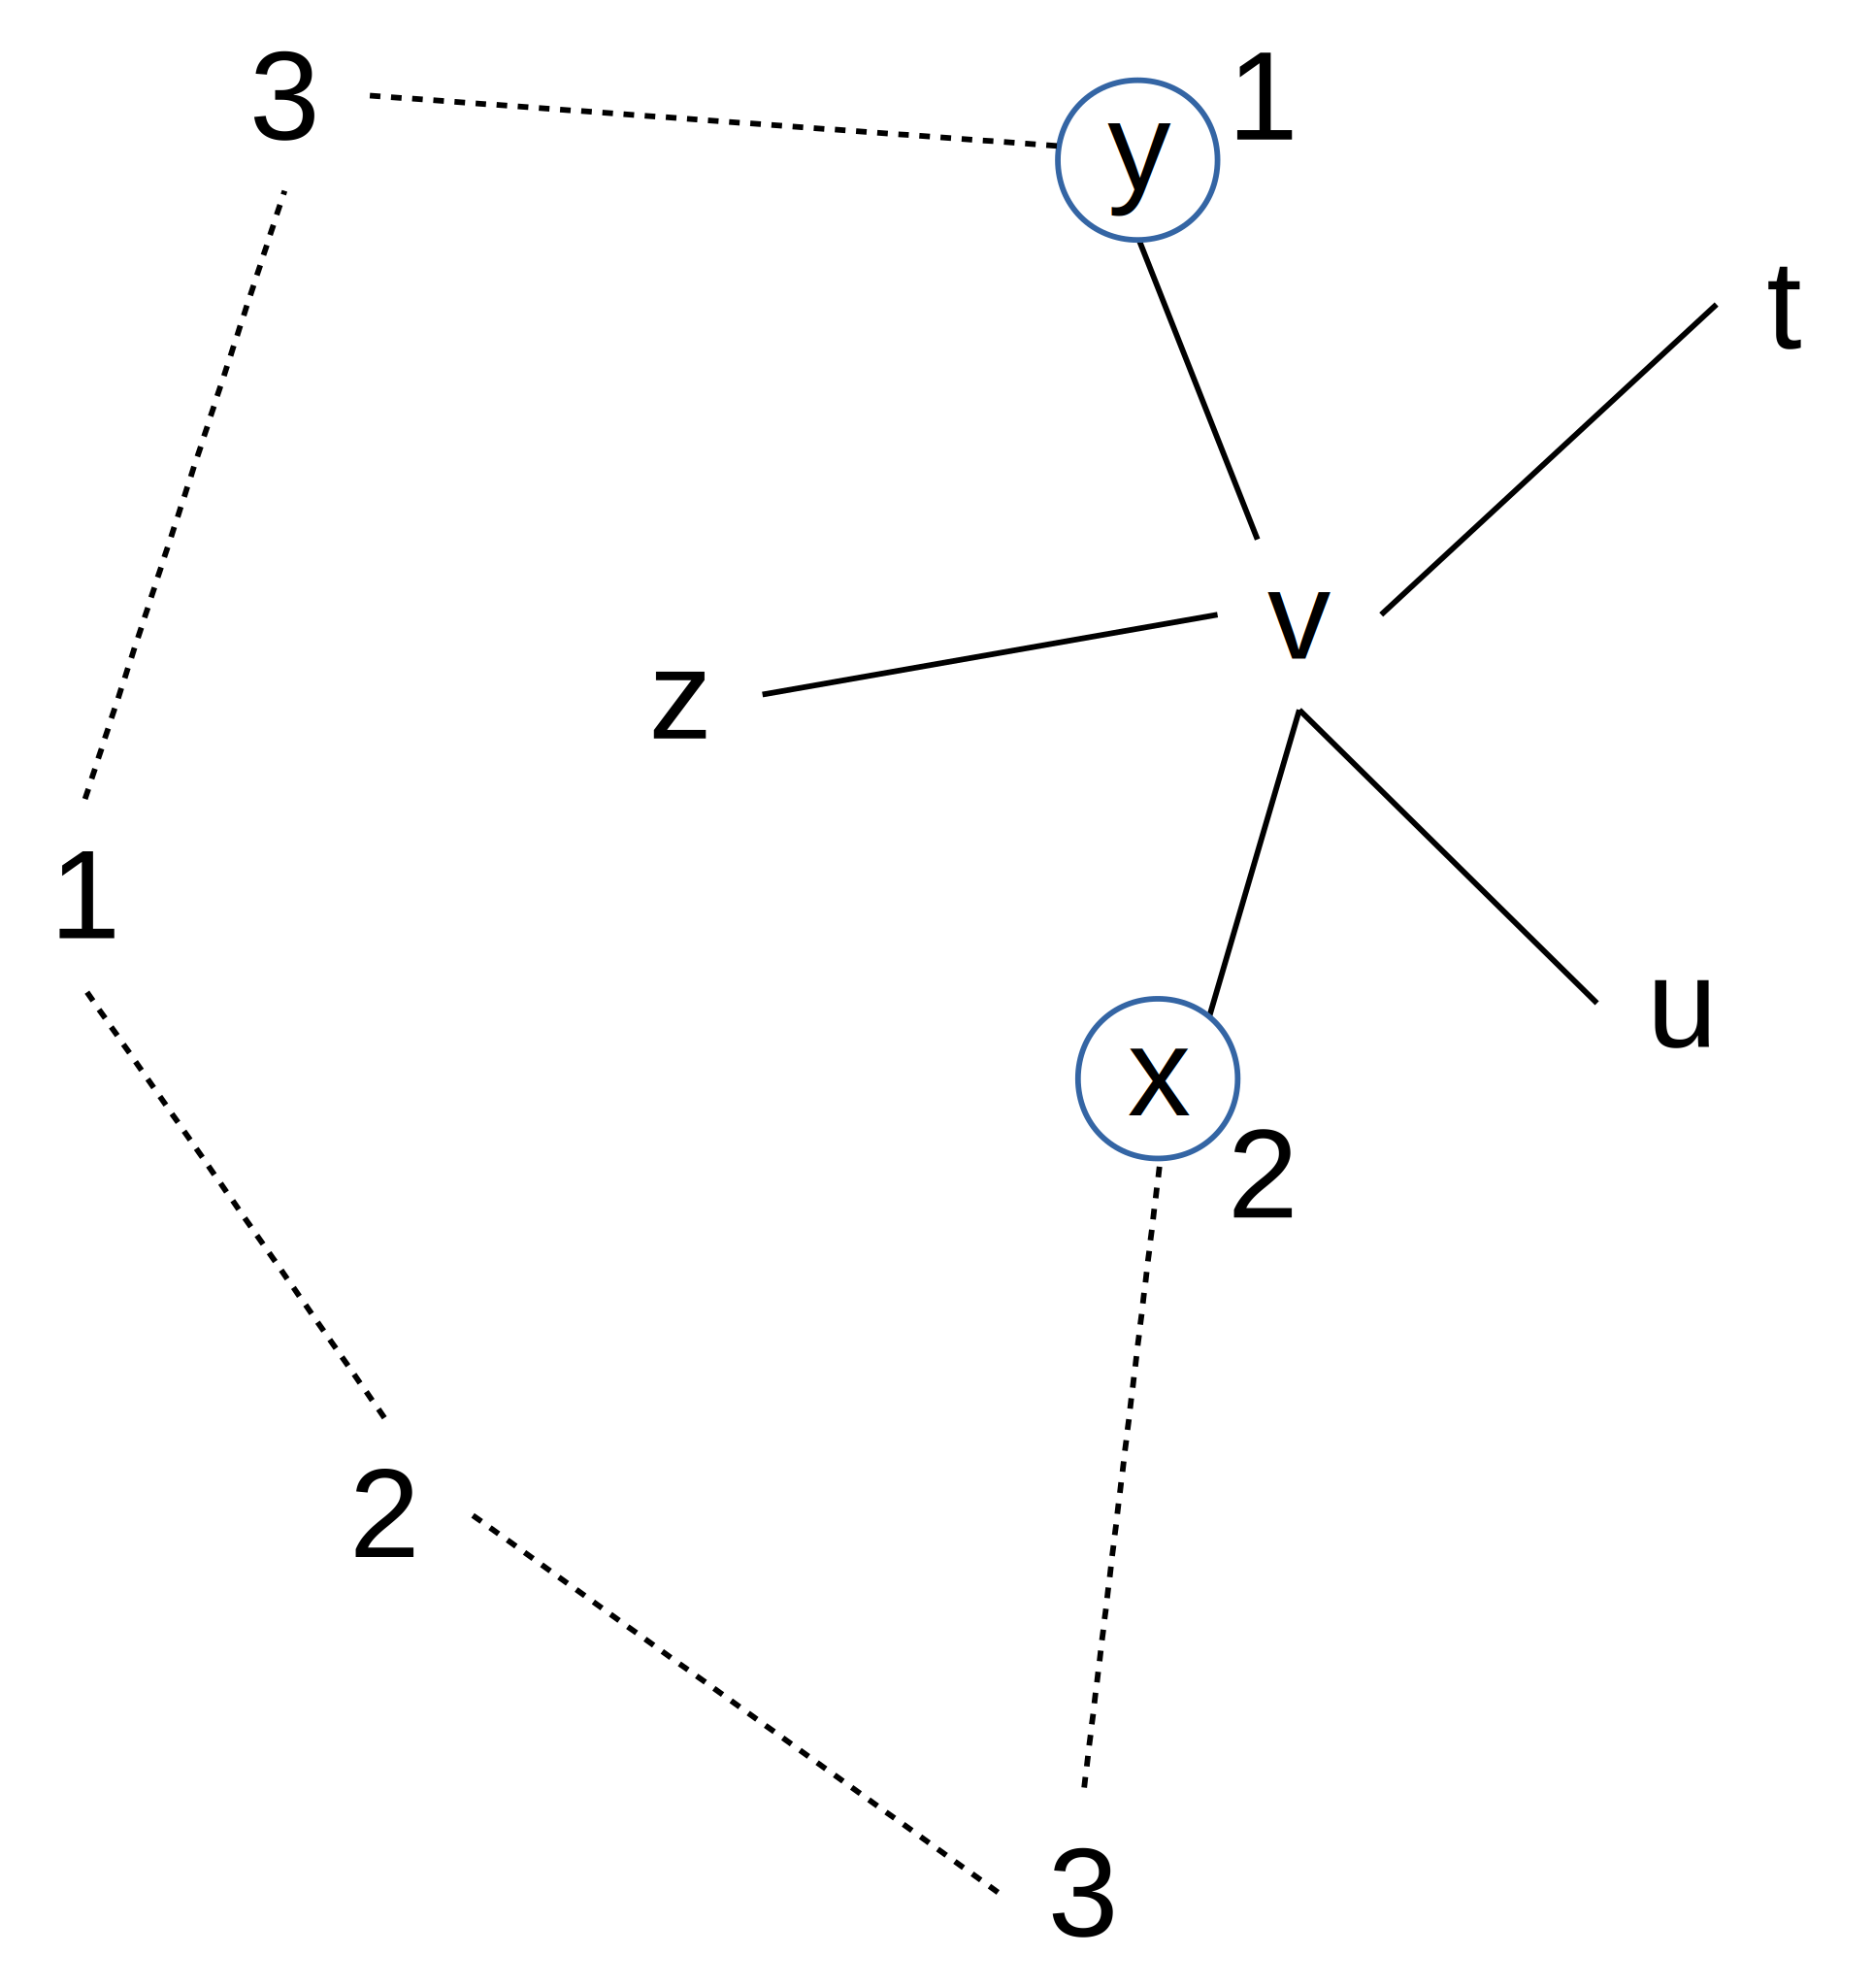
\includegraphics[scale=0.5]{lectures/161125/pix/2.pdf}
                        \begin{itemize}
                            \item betrachte 5-Färbung $\mathcal{C} \colon V(G \setminus \{v\}) \mapsto \{1, \dots, 5\}$, die es nach Rekursion gibt
                            \item betrache $x,y \in V_{xy}$ und sei $V_{xy} \subset V(G)$ die Menge der Knoten mit $\mathcal{C}(x)$- oder $\mathcal{C}(y)$-Färbung
                                \begin{enumerate}
                                    \item es gibt \underline{keinen} Weg von $x \rightsquigarrow y$, der nur Knoten aus $V_{xy}$ nutzt
                                        \begin{itemize}
                                            \item Seien $V'_{xy}$ die $s \in V(G \setminus \{v\})$, die von $x$ nur via $V_{xy}$ erreicht werden
                                            \item Färbe um:
                                            \begin{math}
                                                \mathcal{C'}(s) =
                                                    \begin{cases}
                                                        \mathcal{C}(s) & s \not \in V'_{xy}\\
                                                        \mathcal{C}(y) & s \in V'_{xy}, ~ \mathcal{C}(s) = \mathcal{C}(x)\\
                                                        \mathcal{C}(x) & s \in V'_{xy}, ~ \mathcal{C}(s) = \mathcal{C}(y)
                                                    \end{cases}
                                            \end{math}\\\\
                                            ``Tausche Farben auf $V'_{xy}$'' $\Rightarrow \mathcal{C'}(x) = \mathcal{C'}(y) = \mathcal{C}(y)$
                                        \end{itemize}
                                    \item es gibt einen solchen Pfad $x \rightsquigarrow y$ mit allen Knoten in $V_{xy}$
                                    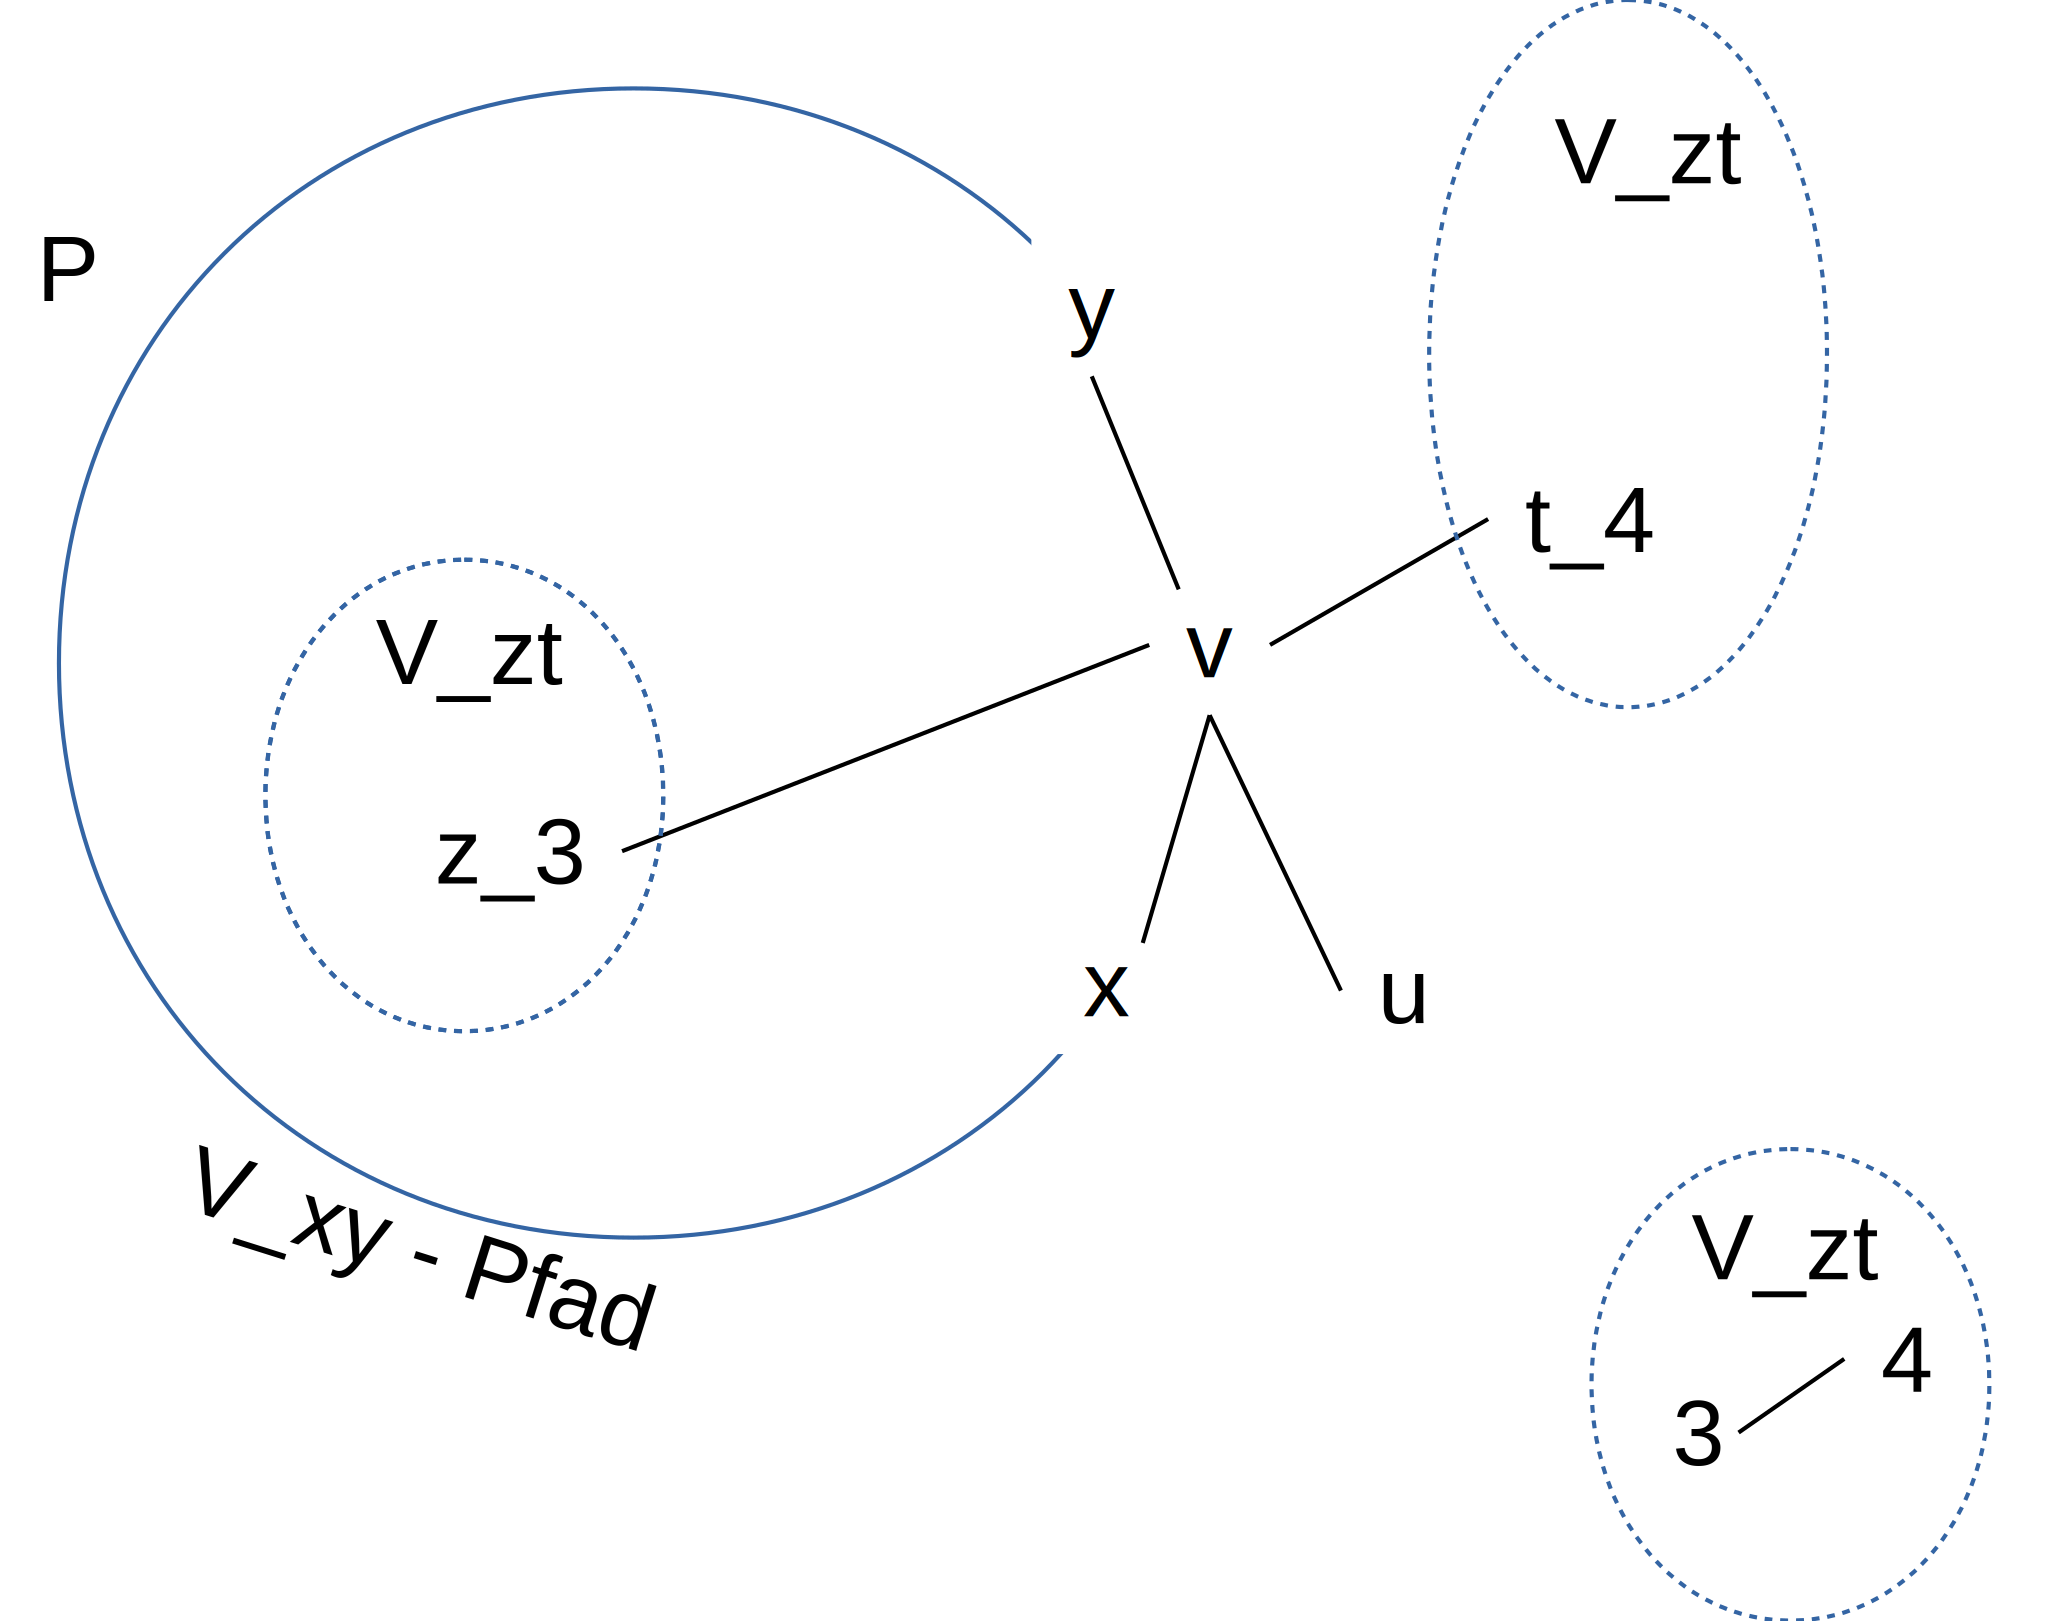
\includegraphics[scale=0.5]{lectures/161125/pix/3.pdf}
                                        \begin{itemize}
                                            \item $V_{zt}$: alle Knoten in $V(G \setminus \{v\})$, die $\mathcal{C}(t)$ oder $\mathcal{C}(z)$ gefärbt sind
                                            \item $V_{xy} \cap V_{zt} = \emptyset$!
                                            \item $V'_{zt}$ kann nur via eines $s \in P$ einen Knoten in $V_{zt} \setminus V'_{zt}$ erreichen
                                        \end{itemize}
                                        Damit lassen sich $z,t$ analog zu Fall (a) färben.
                                \end{enumerate}
                        \end{itemize}
                \end{enumerate}
        \end{description}
    \item[Theorem] Jeder planare Graph ist 4-färbbar
        \begin{description}
            \item[Proof] Es gibt eine Menge von 1936 4-färbbaren Karten, jede nicht Teil eines kleinsten Gegenbeispiels... (Appel, Haken, 1976).
            $\Rightarrow$ Es folgt, dass es kein kleinstes Gegenbeispiel gibt.
        \end{description}
\end{description}

\subsection{Zufallsgraphen}
Sei $G=(V,E)$ mit $V=\{1, \dots, n\}$ fixiert. Wir wollen nun Kanten zufällig auswählen auf dieser fixierten Kantenmenge $\{1, \dots, n\}$, um zufällige Graphen zu generieren. 
Die Menge dieser Zufallsgraphen nennen wir $\mathcal{G}$. \underline{Jede} Kante wird mit Wahrscheinlichkeit $p \in [0, \dots, 1]$ gewählt. 
Sei $G_0$ ein bestimmter Graph. Das Ereignis $\{G_0\}$ mit $G_0$ und m Kanten hat die Wahrscheinlichkeit $p^m \cdot (1-p)^{{n \over 2}-m}$. 
Wahrscheinlichkeitsmaß auf 
$\mathcal{G} ~ \forall e \in [v]^2$\\
$\Omega_e=\{0_e, 1_e\}$\\
$\mathbb{P}(\{1_e\})=p$\\
$\mathbb{P}(\{0_e\})=1-p$\\
$\Omega_\mathcal{G} = \prod\limits_{e \in [v]^2} \Omega_e$

\begin{description}
    \item[Beispiele] Fixiere Graph $H$, $V(H) = V(G)$, ist $H \leqslant G$? \\
        Mit $p^l$, $|E(H)| = l$, $|V(H)| = k$, aber falls $H$ induzierter Teilgraph von $G$ sein soll? \\
         - Nur $p^l (1-p)^{\binom{k}{2} - l}$. \\
        Und was ist mit Subgraph-Isomorphismus?
        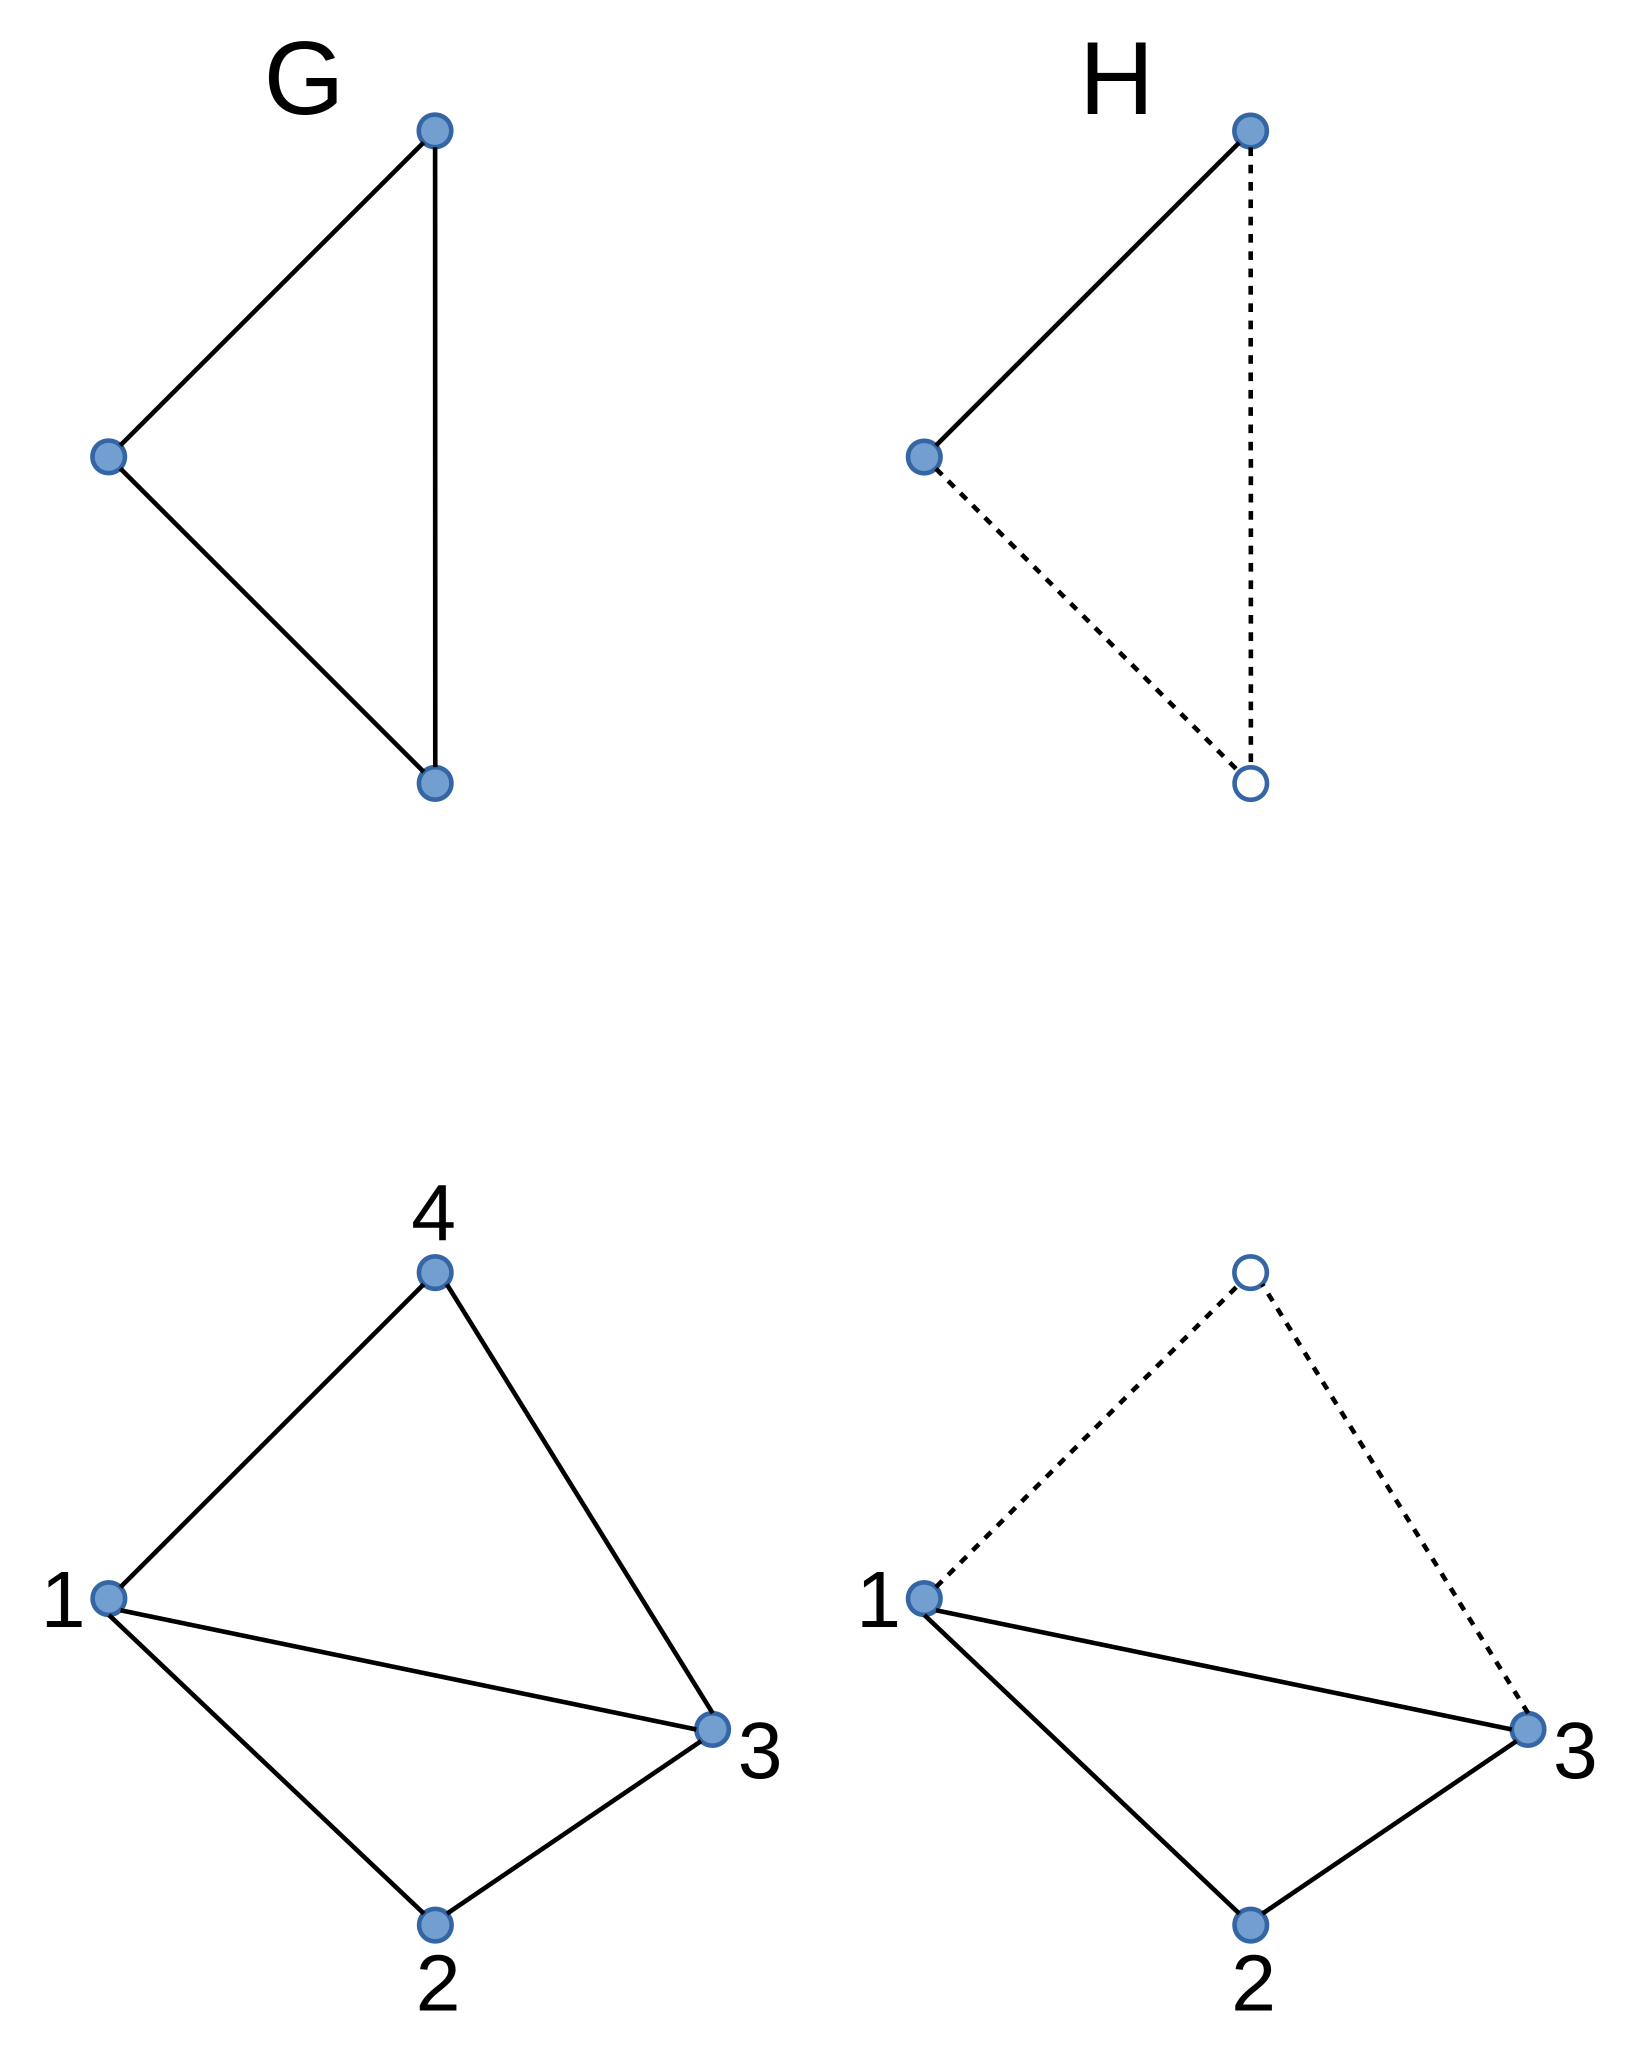
\includegraphics[scale=0.5]{lectures/161125/pix/4.pdf}
        \begin{itemize}
            \item Ereignismengen überlappen
            \item kompliziert
        \end{itemize}
\end{description}

\subsection{Eigenschaften fast aller Graphen}
Falls die Wahrscheinlichkeit, dass $P(G \in \mathcal{G}) \rightarrow 1$ für $n \rightarrow \infty$, dann geschieht $G$ fast sicher.
\begin{description}
    \item[Pro:] Gegeben jedes $H$ als Isomorphie-Klasse, $n \rightarrow \infty$ und $p \in ]0,1[ = (0,1)$, induzierte Kopie von $H$. 
    Dann haben fast alle $G$ in $\mathcal{G}(n,p)$ haben mindestens eine induzierte Kopie von $H$.
    \item[Prf:] Sei $H$ gegeben, $K=V(H)$. Sei $K \leqslant n$. $H$ ist (subgraph-) isomorph zu $G$ mit Wahrscheinlichkeit $r < 0$ ($G$ ist zufällig!). 
        Teile $G$ in $\lfloor {n \over k} \rfloor$ Teilgraphen, um genau so viele ``Versuche'' (für $r > 0$) zu haben. 
        $P(H \not \subseteq G$ induziert) $\leqslant (1-r)^{\lfloor {n \over k} \rfloor} \xrightarrow{n \rightarrow \infty} 0$
\end{description}


\newpage

\section{Vorlesung 25.11.2016}
\subsection{Färbung von Graphen}
\subsubsection{Vertexfärbung}
Zwei durch eine Kante verbundene Knoten haben unterschiedliche Farben.\\
Beispiel wäre eine Landkarte auf der mit so wenig wie möglich Farben die Länder ausgemalt werden, ohne zwei benachbarte Länder gleichfarbig zu haben. Hierbei entspricht jede Facette einen Knoten.\\
\includegraphics[width=0.4\textwidth]{lectures/161125/pix/Vertexfaerbung}
\begin{description}
    \item[Vertexfärbung] Eine Vertexfärbung eines Graphen $G=(V,E)$ ist eine Abbildung $\mathcal{C} \colon V \mapsto \mathcal{S}$, mit $\mathcal{S}=$ Menge der Farben. Es gilt, dass $\mathcal{C}(v) \neq \mathcal{C}(w)$, mit $w,v \in \mathcal{S}$, wenn $v$ und $w$ adjazent ($\{v,w\} \in E$) sind. Die Elemente von $\mathcal{S}$ heißen \emph{Farben}.
    \item[k-Färbung] Ein Graph $G$ ist $k$-färbbar, wenn es für eine Abbildung $\mathcal{C}$ eine Menge $\mathcal{S}=\{1,\dots,k\}$ gibt.
    \item[Chromatische Zahl] Eine chromatische Zahl $\chi(G)$ ist die kleinste natürliche Zahl $k$, sodass G $k$-färbbar ist. $\chi(G) \leqslant \Delta(G) + 1$, mit $\Delta(G) = $ maximaler Grad von $G$
        \begin{description}
            \item[Proof (greedy)] Färbe $v_i$ der Vertices $v_1 \dots v_n$ mit der kleinsten Farbe, die nicht von einem Nachbarn von $v_i$ benutzt wird. Da wir max. $\Delta(G)$ viele Nachbarn für $v_i$ haben, gibt es immer eine freie Farbe.
        \end{description}
        $\chi(G) \geqslant$ Größe der größten Clique
    \item[Lemma] Für jeden einfachen planaren Graphen $G$ ist der Durchschnittsgrad $d(G) < 6$
        \begin{description}
            \item[Proof] $d(G) = 2 \cdot {|E| \over |V|}$ mit $|V| \leqslant 3$, $|E| \leqslant 3  \cdot |V| - 6$, dann $d(G) \leqslant {2(3 \cdot |V|-6) \over |V|} = 6-{12 \over |V|}$
        \end{description}
    \item[Theorem] Jeder simple planare Graph $G$ hat $\chi(G) \leqslant 6$
        \begin{description}
            \item[Proof] Annahme: Jeder simple planare Graph mit $|V| = n$ ist $6$-färbbar.
            \begin{itemize}
                \item Sei $G$ hiermit ein simpler planarer Graph mit $|V| = n+1$
                \item Vom Lemma wissen wir, dass $w \in V$ mit $d(w) \leqslant 5$ existiert
                \item Sei $G' = G \setminus \{w\}$. Via Induktionshypothese ist $G'$ 6-färbbar. Das tun wir dann.
                \item Färbe $w$ mit der (min.) freien Farbe, um $G$ zu färben
            \end{itemize}
        \end{description}
    \item[Theorem] Für jeden simplen planaren Graphen $G$ gilt, dass $\chi(G) \leqslant 5$
        \begin{description}
            \item[Proof] Sei $G=(V,E)$ planar
                \begin{enumerate}
                    \item Falls $|V| \leqslant 5 \rightarrow$ trivial
                    \item Für alle $v \in V(G)$ mit $deg(v) < 5$, färbe $v$ und arbeite mit $G \setminus \{v\}$
                    \item $G$ hat Vertex $v$ mit $deg(v) = 5$
                        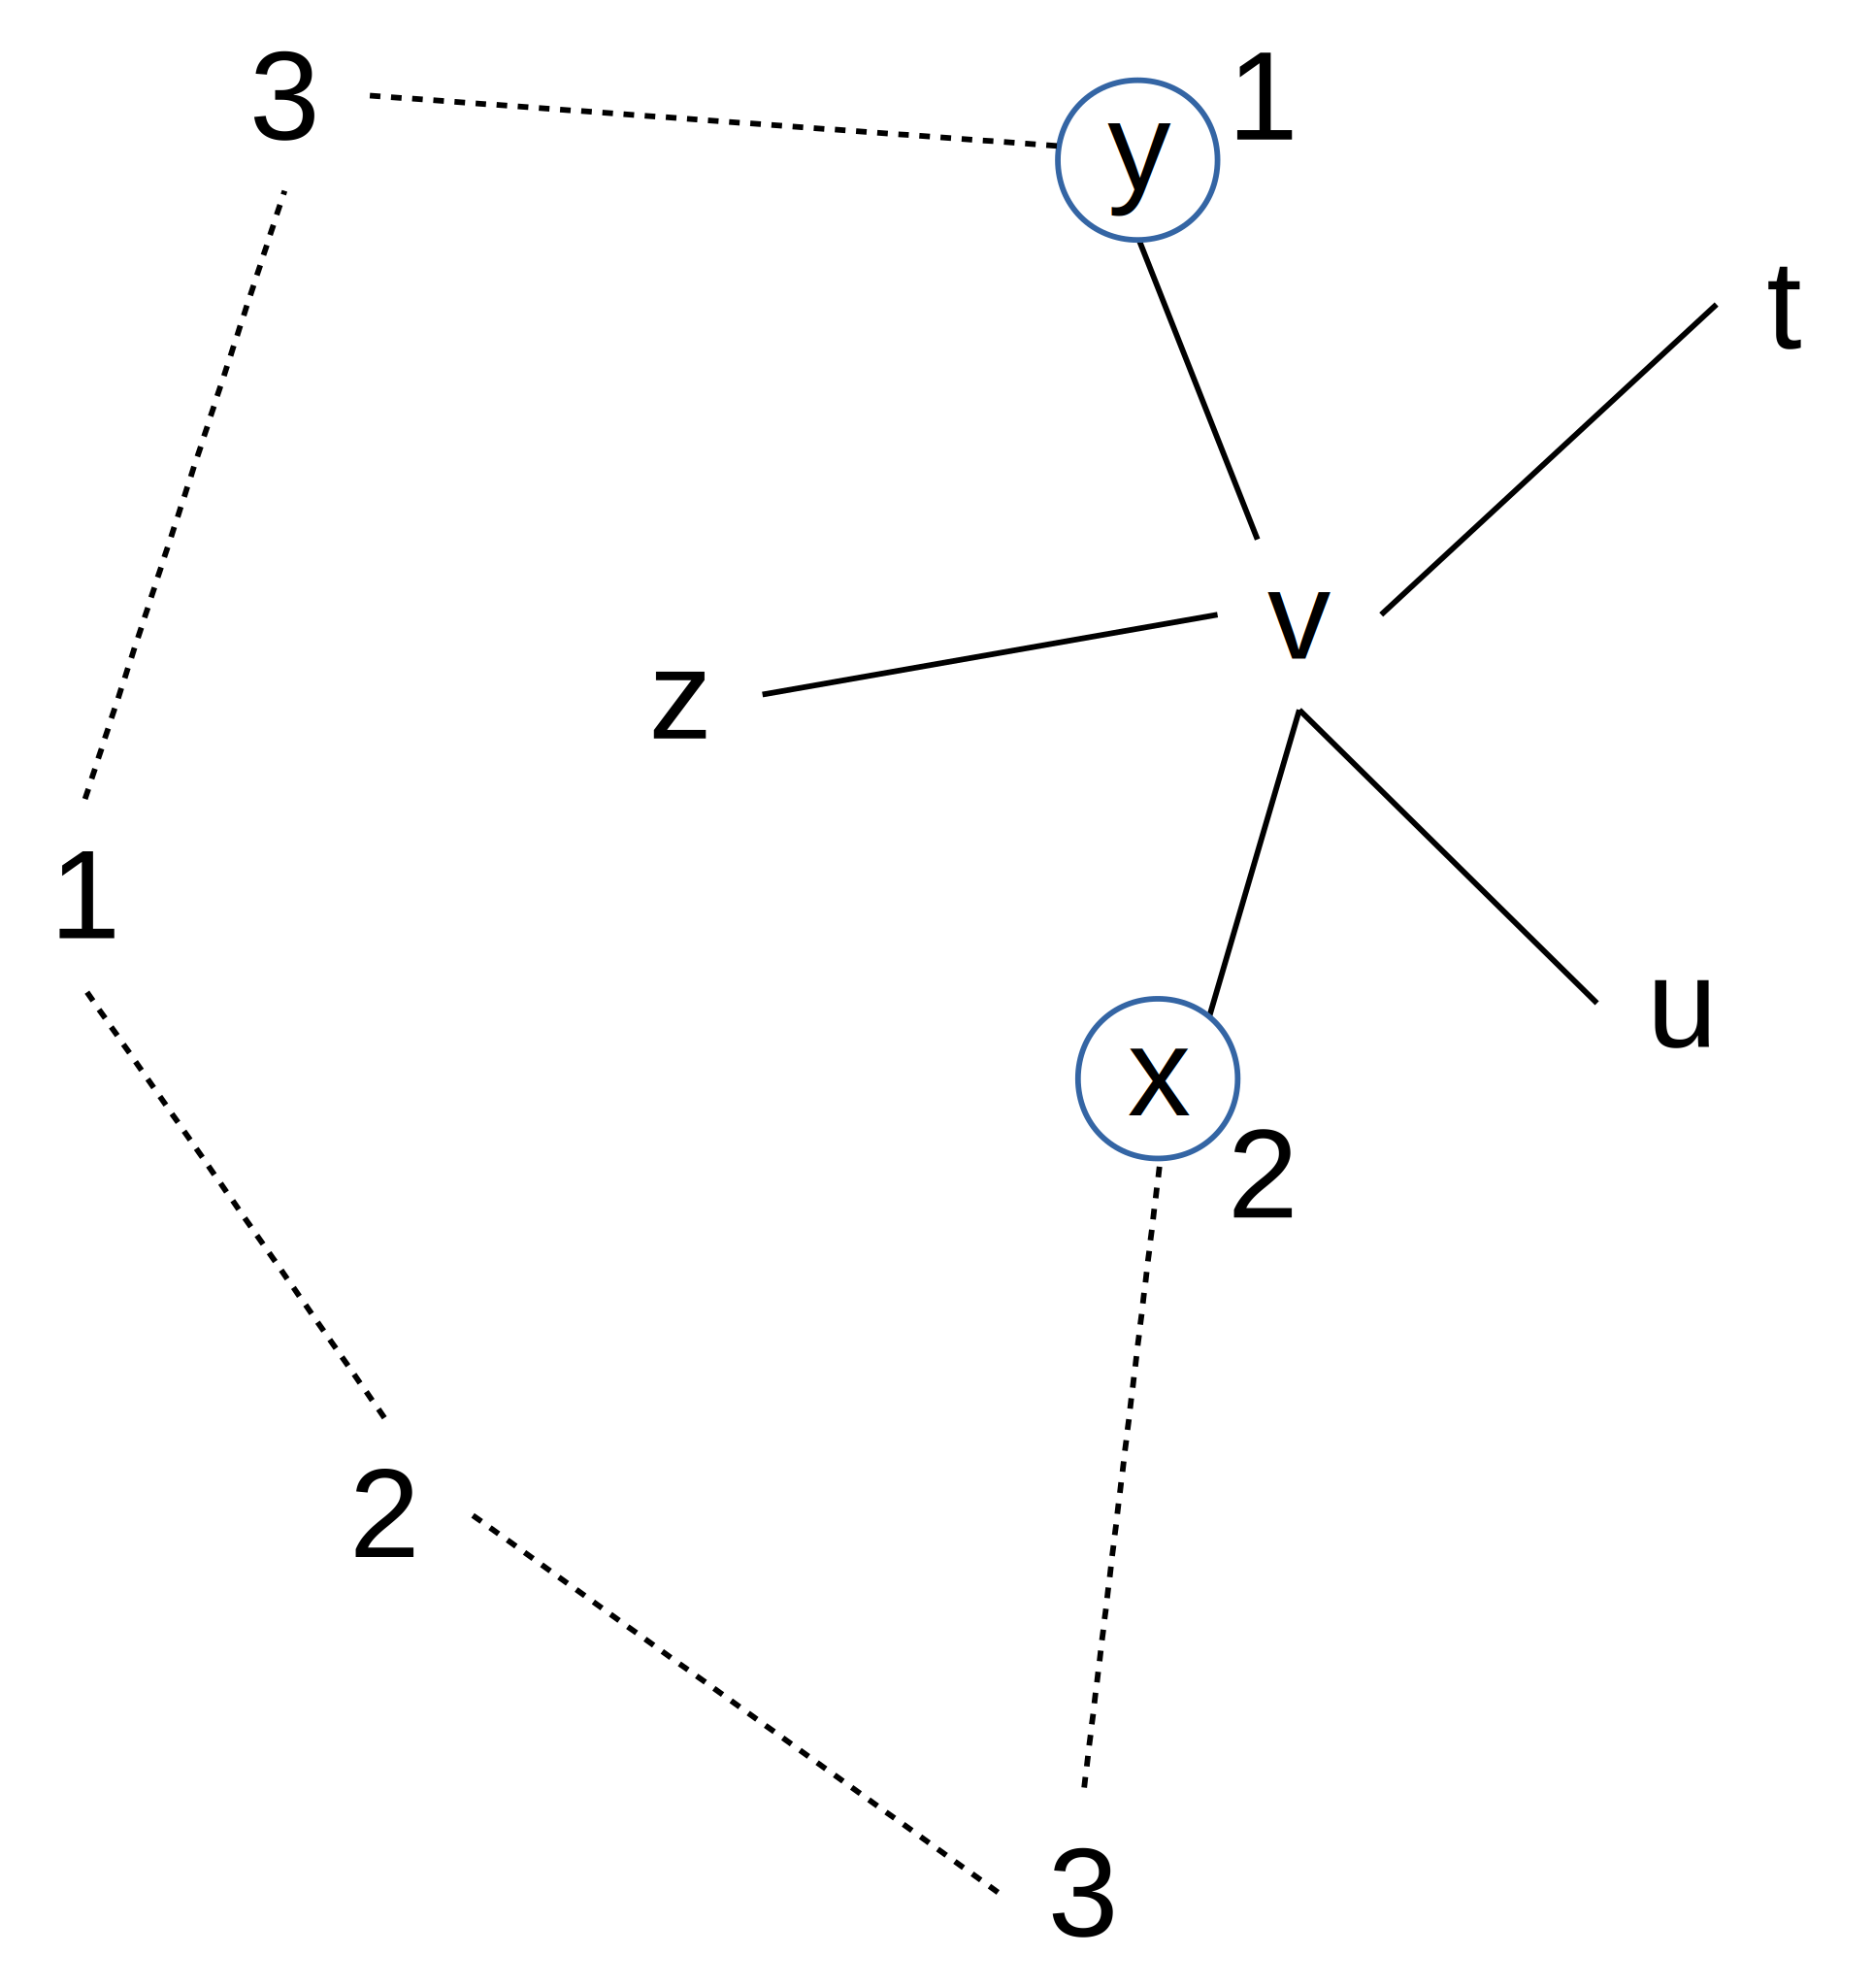
\includegraphics[scale=0.5]{lectures/161125/pix/2.pdf}
                        \begin{itemize}
                            \item betrachte 5-Färbung $\mathcal{C} \colon V(G \setminus \{v\}) \mapsto \{1, \dots, 5\}$, die es nach Rekursion gibt
                            \item betrache $x,y \in V_{xy}$ und sei $V_{xy} \subset V(G)$ die Menge der Knoten mit $\mathcal{C}(x)$- oder $\mathcal{C}(y)$-Färbung
                                \begin{enumerate}
                                    \item es gibt \underline{keinen} Weg von $x \rightsquigarrow y$, der nur Knoten aus $V_{xy}$ nutzt
                                        \begin{itemize}
                                            \item Seien $V'_{xy}$ die $s \in V(G \setminus \{v\})$, die von $x$ nur via $V_{xy}$ erreicht werden
                                            \item Färbe um:
                                            \begin{math}
                                                \mathcal{C'}(s) =
                                                    \begin{cases}
                                                        \mathcal{C}(s) & s \not \in V'_{xy}\\
                                                        \mathcal{C}(y) & s \in V'_{xy}, ~ \mathcal{C}(s) = \mathcal{C}(x)\\
                                                        \mathcal{C}(x) & s \in V'_{xy}, ~ \mathcal{C}(s) = \mathcal{C}(y)
                                                    \end{cases}
                                            \end{math}\\\\
                                            ``Tausche Farben auf $V'_{xy}$'' $\Rightarrow \mathcal{C'}(x) = \mathcal{C'}(y) = \mathcal{C}(y)$
                                        \end{itemize}
                                    \item es gibt einen solchen Pfad $x \rightsquigarrow y$ mit allen Knoten in $V_{xy}$
                                    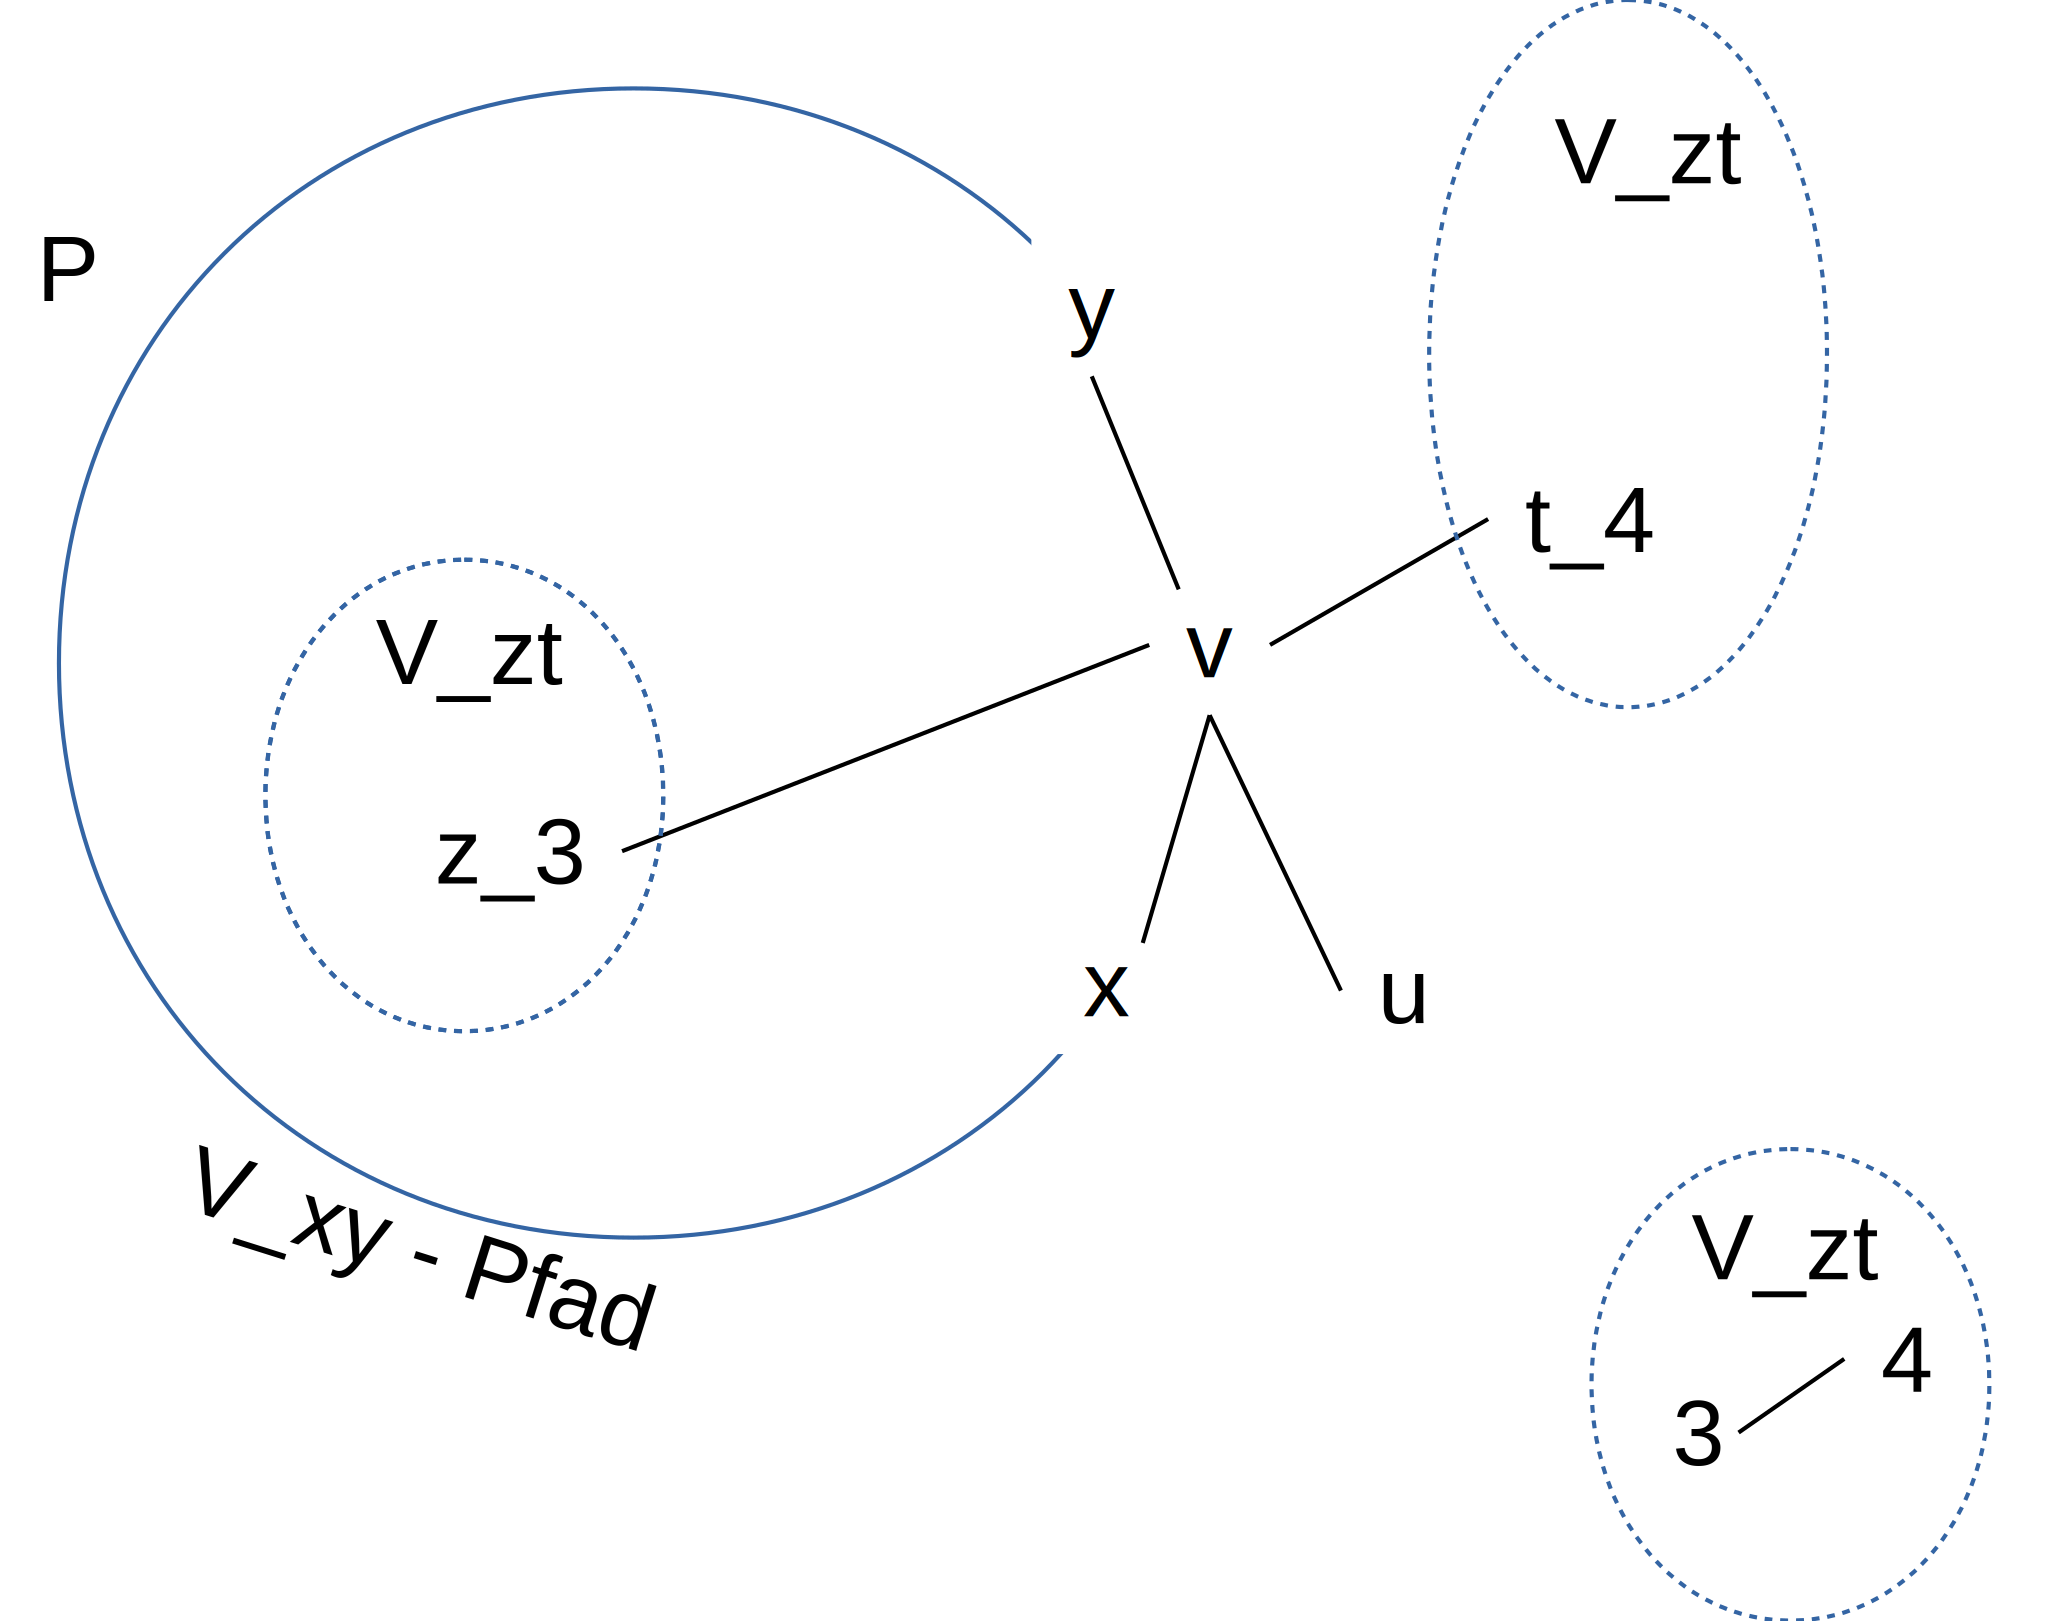
\includegraphics[scale=0.5]{lectures/161125/pix/3.pdf}
                                        \begin{itemize}
                                            \item $V_{zt}$: alle Knoten in $V(G \setminus \{v\})$, die $\mathcal{C}(t)$ oder $\mathcal{C}(z)$ gefärbt sind
                                            \item $V_{xy} \cap V_{zt} = \emptyset$!
                                            \item $V'_{zt}$ kann nur via eines $s \in P$ einen Knoten in $V_{zt} \setminus V'_{zt}$ erreichen
                                        \end{itemize}
                                        Damit lassen sich $z,t$ analog zu Fall (a) färben.
                                \end{enumerate}
                        \end{itemize}
                \end{enumerate}
        \end{description}
    \item[Theorem] Jeder planare Graph ist 4-färbbar
        \begin{description}
            \item[Proof] Es gibt eine Menge von 1936 4-färbbaren Karten, jede nicht Teil eines kleinsten Gegenbeispiels... (Appel, Haken, 1976).
            $\Rightarrow$ Es folgt, dass es kein kleinstes Gegenbeispiel gibt.
        \end{description}
\end{description}

\subsection{Zufallsgraphen}
Sei $G=(V,E)$ mit $V=\{1, \dots, n\}$ fixiert. Wir wollen nun Kanten zufällig auswählen auf dieser fixierten Kantenmenge $\{1, \dots, n\}$, um zufällige Graphen zu generieren. 
Die Menge dieser Zufallsgraphen nennen wir $\mathcal{G}$. \underline{Jede} Kante wird mit Wahrscheinlichkeit $p \in [0, \dots, 1]$ gewählt. 
Sei $G_0$ ein bestimmter Graph. Das Ereignis $\{G_0\}$ mit $G_0$ und m Kanten hat die Wahrscheinlichkeit $p^m \cdot (1-p)^{{n \over 2}-m}$. 
Wahrscheinlichkeitsmaß auf 
$\mathcal{G} ~ \forall e \in [v]^2$\\
$\Omega_e=\{0_e, 1_e\}$\\
$\mathbb{P}(\{1_e\})=p$\\
$\mathbb{P}(\{0_e\})=1-p$\\
$\Omega_\mathcal{G} = \prod\limits_{e \in [v]^2} \Omega_e$

\begin{description}
    \item[Beispiele] Fixiere Graph $H$, $V(H) = V(G)$, ist $H \leqslant G$? \\
        Mit $p^l$, $|E(H)| = l$, $|V(H)| = k$, aber falls $H$ induzierter Teilgraph von $G$ sein soll? \\
         - Nur $p^l (1-p)^{\binom{k}{2} - l}$. \\
        Und was ist mit Subgraph-Isomorphismus?
        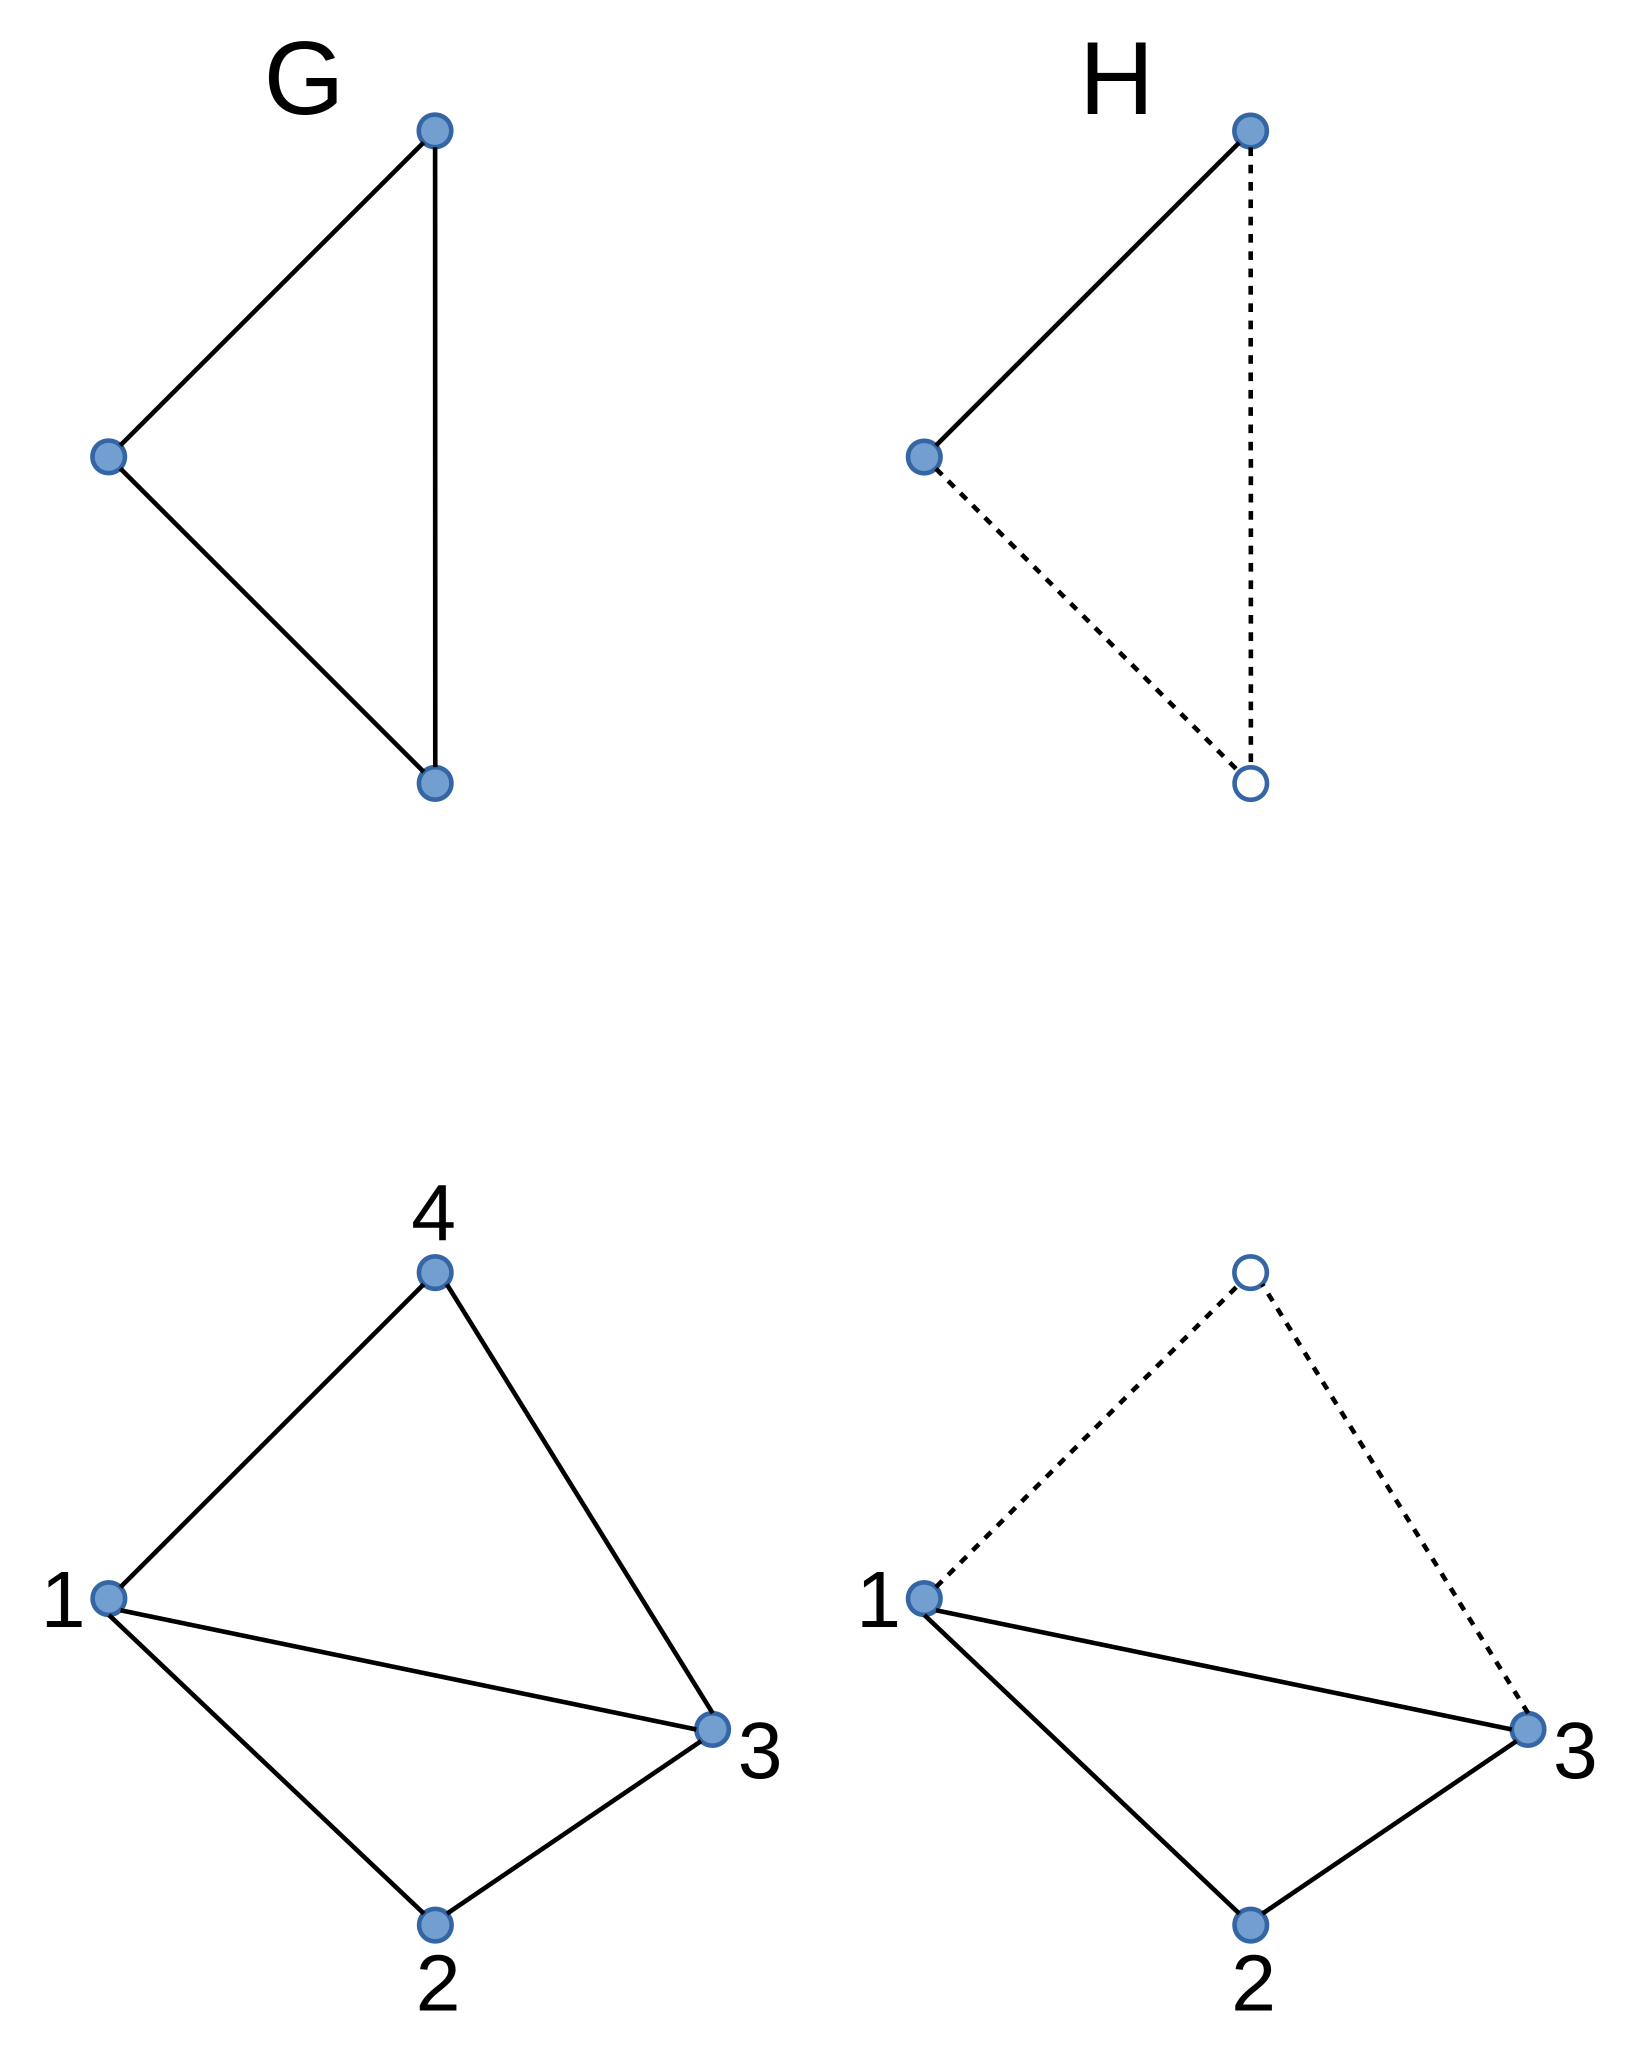
\includegraphics[scale=0.5]{lectures/161125/pix/4.pdf}
        \begin{itemize}
            \item Ereignismengen überlappen
            \item kompliziert
        \end{itemize}
\end{description}

\subsection{Eigenschaften fast aller Graphen}
Falls die Wahrscheinlichkeit, dass $P(G \in \mathcal{G}) \rightarrow 1$ für $n \rightarrow \infty$, dann geschieht $G$ fast sicher.
\begin{description}
    \item[Pro:] Gegeben jedes $H$ als Isomorphie-Klasse, $n \rightarrow \infty$ und $p \in ]0,1[ = (0,1)$, induzierte Kopie von $H$. 
    Dann haben fast alle $G$ in $\mathcal{G}(n,p)$ haben mindestens eine induzierte Kopie von $H$.
    \item[Prf:] Sei $H$ gegeben, $K=V(H)$. Sei $K \leqslant n$. $H$ ist (subgraph-) isomorph zu $G$ mit Wahrscheinlichkeit $r < 0$ ($G$ ist zufällig!). 
        Teile $G$ in $\lfloor {n \over k} \rfloor$ Teilgraphen, um genau so viele ``Versuche'' (für $r > 0$) zu haben. 
        $P(H \not \subseteq G$ induziert) $\leqslant (1-r)^{\lfloor {n \over k} \rfloor} \xrightarrow{n \rightarrow \infty} 0$
\end{description}


\newpage

\section{Vorlesung 25.11.2016}
\subsection{Färbung von Graphen}
\subsubsection{Vertexfärbung}
Zwei durch eine Kante verbundene Knoten haben unterschiedliche Farben.\\
Beispiel wäre eine Landkarte auf der mit so wenig wie möglich Farben die Länder ausgemalt werden, ohne zwei benachbarte Länder gleichfarbig zu haben. Hierbei entspricht jede Facette einen Knoten.\\
\includegraphics[width=0.4\textwidth]{lectures/161125/pix/Vertexfaerbung}
\begin{description}
    \item[Vertexfärbung] Eine Vertexfärbung eines Graphen $G=(V,E)$ ist eine Abbildung $\mathcal{C} \colon V \mapsto \mathcal{S}$, mit $\mathcal{S}=$ Menge der Farben. Es gilt, dass $\mathcal{C}(v) \neq \mathcal{C}(w)$, mit $w,v \in \mathcal{S}$, wenn $v$ und $w$ adjazent ($\{v,w\} \in E$) sind. Die Elemente von $\mathcal{S}$ heißen \emph{Farben}.
    \item[k-Färbung] Ein Graph $G$ ist $k$-färbbar, wenn es für eine Abbildung $\mathcal{C}$ eine Menge $\mathcal{S}=\{1,\dots,k\}$ gibt.
    \item[Chromatische Zahl] Eine chromatische Zahl $\chi(G)$ ist die kleinste natürliche Zahl $k$, sodass G $k$-färbbar ist. $\chi(G) \leqslant \Delta(G) + 1$, mit $\Delta(G) = $ maximaler Grad von $G$
        \begin{description}
            \item[Proof (greedy)] Färbe $v_i$ der Vertices $v_1 \dots v_n$ mit der kleinsten Farbe, die nicht von einem Nachbarn von $v_i$ benutzt wird. Da wir max. $\Delta(G)$ viele Nachbarn für $v_i$ haben, gibt es immer eine freie Farbe.
        \end{description}
        $\chi(G) \geqslant$ Größe der größten Clique
    \item[Lemma] Für jeden einfachen planaren Graphen $G$ ist der Durchschnittsgrad $d(G) < 6$
        \begin{description}
            \item[Proof] $d(G) = 2 \cdot {|E| \over |V|}$ mit $|V| \leqslant 3$, $|E| \leqslant 3  \cdot |V| - 6$, dann $d(G) \leqslant {2(3 \cdot |V|-6) \over |V|} = 6-{12 \over |V|}$
        \end{description}
    \item[Theorem] Jeder simple planare Graph $G$ hat $\chi(G) \leqslant 6$
        \begin{description}
            \item[Proof] Annahme: Jeder simple planare Graph mit $|V| = n$ ist $6$-färbbar.
            \begin{itemize}
                \item Sei $G$ hiermit ein simpler planarer Graph mit $|V| = n+1$
                \item Vom Lemma wissen wir, dass $w \in V$ mit $d(w) \leqslant 5$ existiert
                \item Sei $G' = G \setminus \{w\}$. Via Induktionshypothese ist $G'$ 6-färbbar. Das tun wir dann.
                \item Färbe $w$ mit der (min.) freien Farbe, um $G$ zu färben
            \end{itemize}
        \end{description}
    \item[Theorem] Für jeden simplen planaren Graphen $G$ gilt, dass $\chi(G) \leqslant 5$
        \begin{description}
            \item[Proof] Sei $G=(V,E)$ planar
                \begin{enumerate}
                    \item Falls $|V| \leqslant 5 \rightarrow$ trivial
                    \item Für alle $v \in V(G)$ mit $deg(v) < 5$, färbe $v$ und arbeite mit $G \setminus \{v\}$
                    \item $G$ hat Vertex $v$ mit $deg(v) = 5$
                        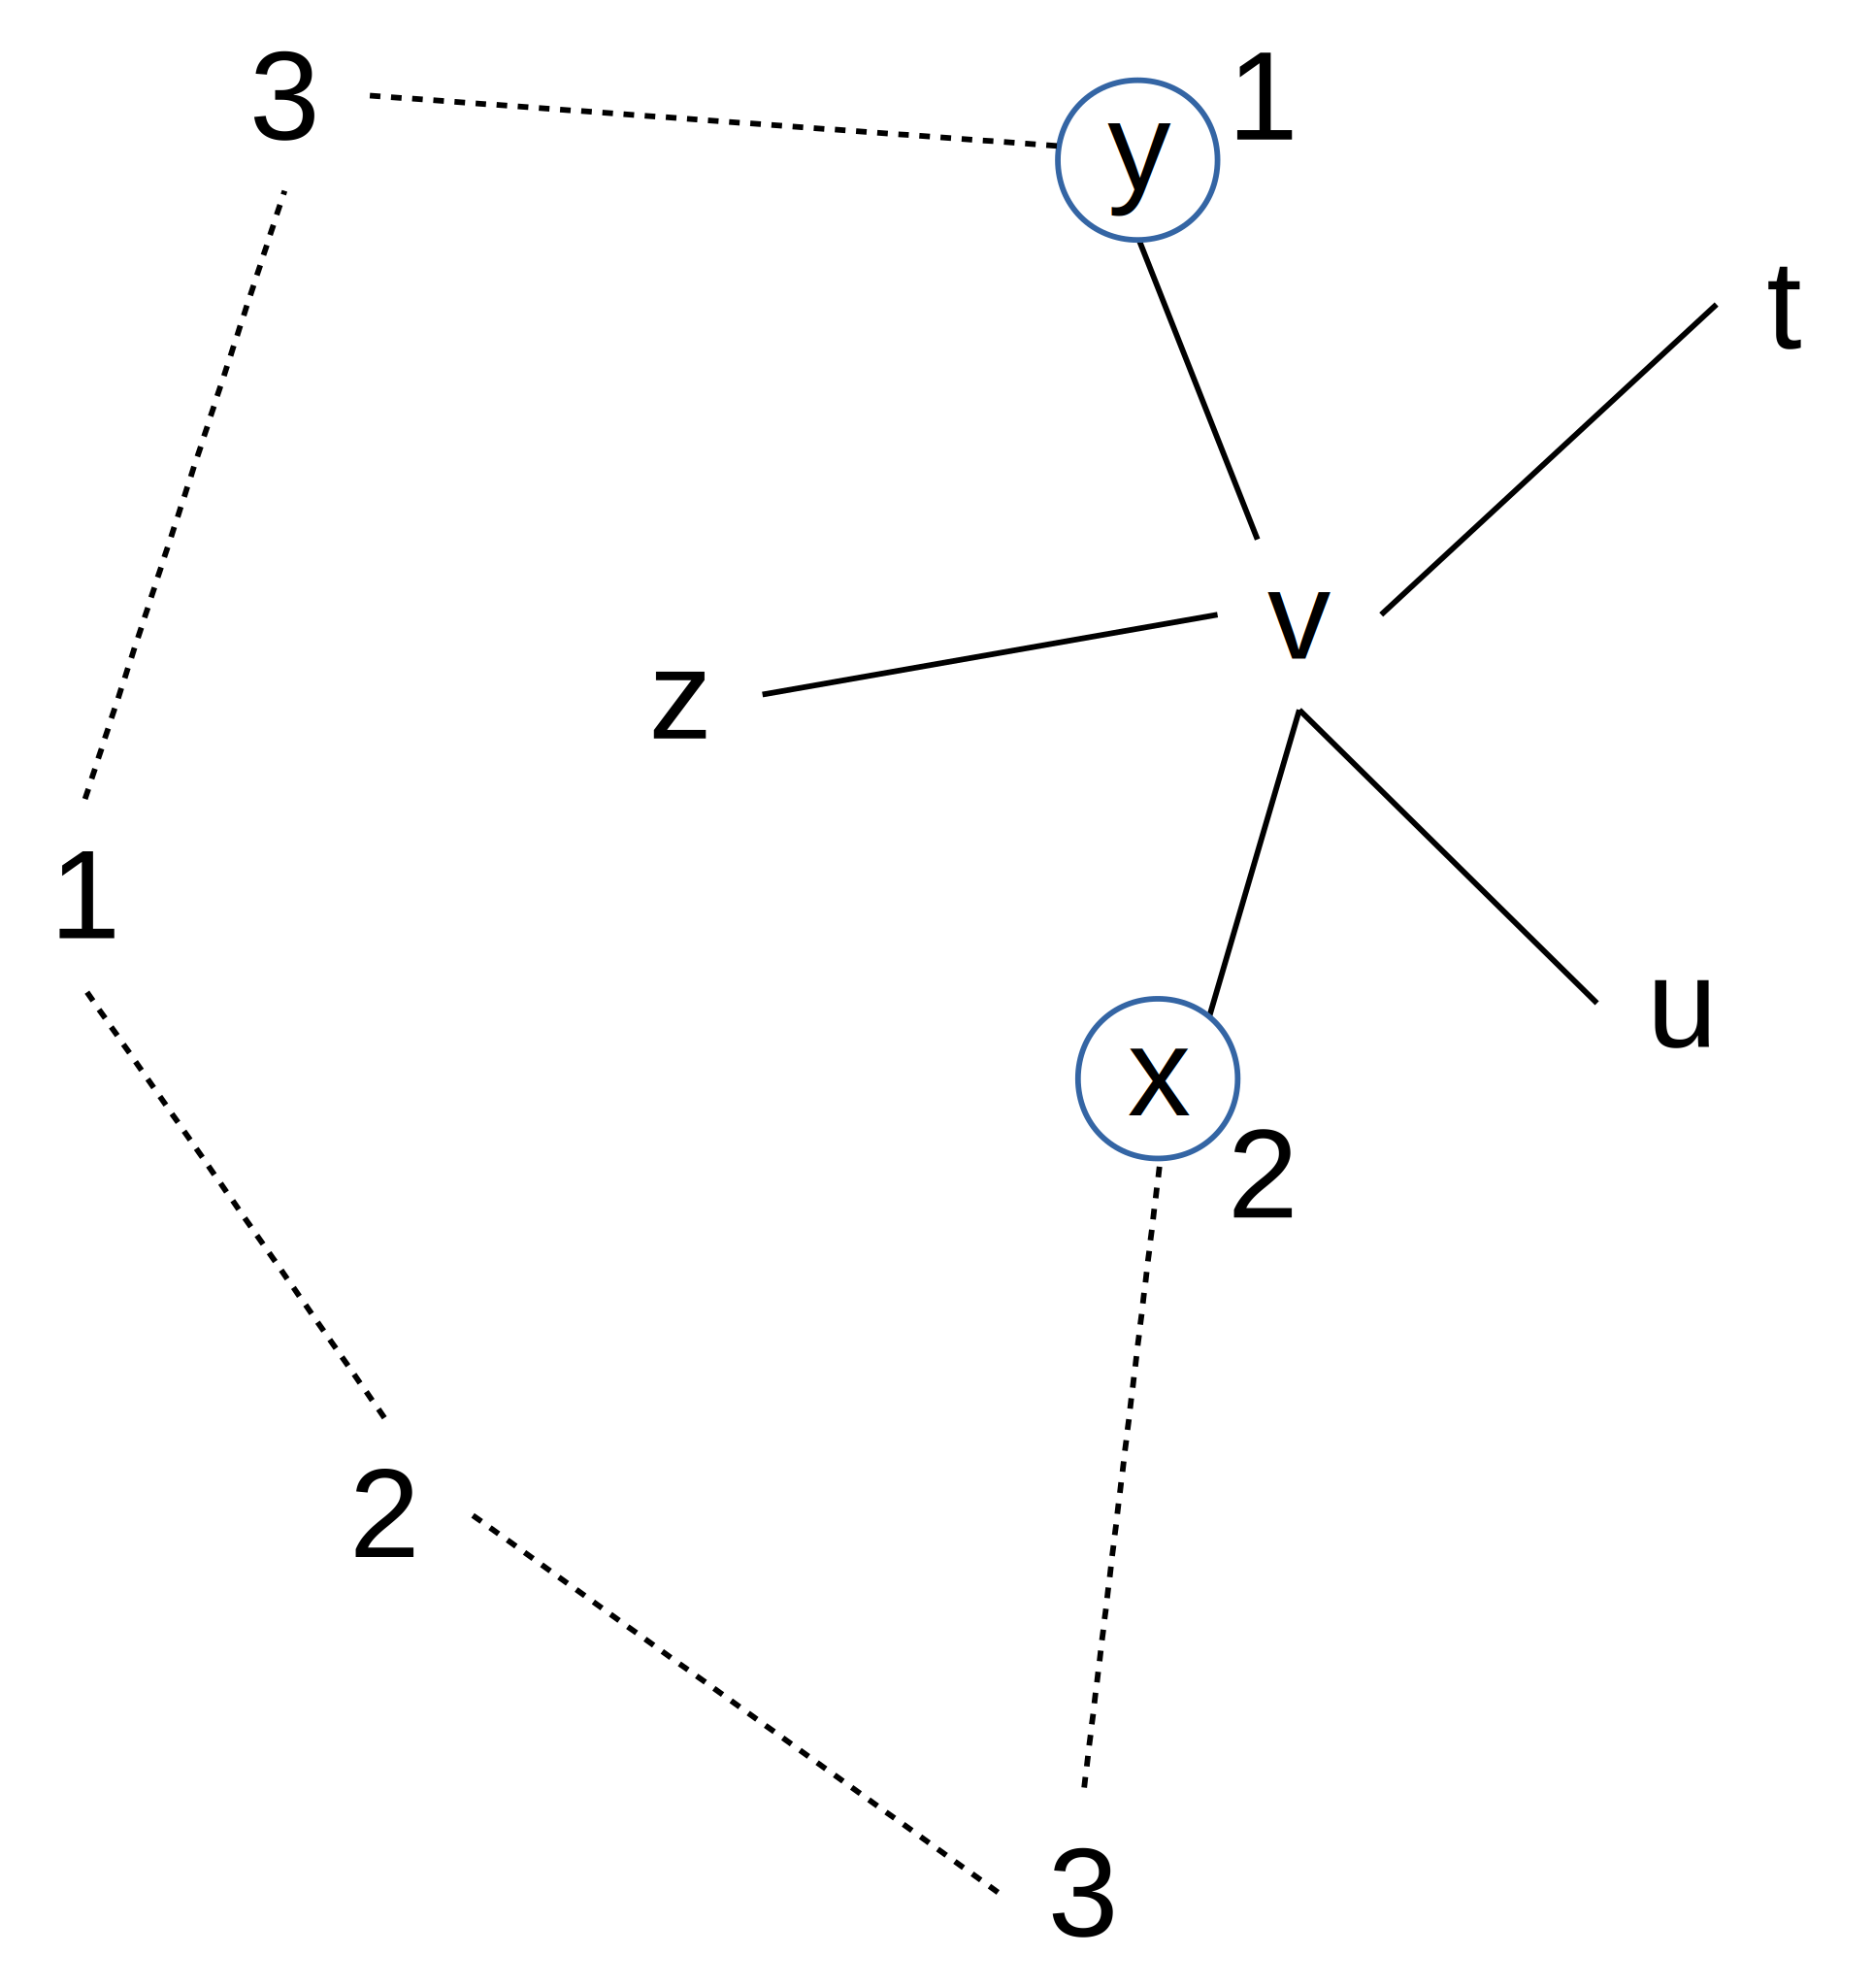
\includegraphics[scale=0.5]{lectures/161125/pix/2.pdf}
                        \begin{itemize}
                            \item betrachte 5-Färbung $\mathcal{C} \colon V(G \setminus \{v\}) \mapsto \{1, \dots, 5\}$, die es nach Rekursion gibt
                            \item betrache $x,y \in V_{xy}$ und sei $V_{xy} \subset V(G)$ die Menge der Knoten mit $\mathcal{C}(x)$- oder $\mathcal{C}(y)$-Färbung
                                \begin{enumerate}
                                    \item es gibt \underline{keinen} Weg von $x \rightsquigarrow y$, der nur Knoten aus $V_{xy}$ nutzt
                                        \begin{itemize}
                                            \item Seien $V'_{xy}$ die $s \in V(G \setminus \{v\})$, die von $x$ nur via $V_{xy}$ erreicht werden
                                            \item Färbe um:
                                            \begin{math}
                                                \mathcal{C'}(s) =
                                                    \begin{cases}
                                                        \mathcal{C}(s) & s \not \in V'_{xy}\\
                                                        \mathcal{C}(y) & s \in V'_{xy}, ~ \mathcal{C}(s) = \mathcal{C}(x)\\
                                                        \mathcal{C}(x) & s \in V'_{xy}, ~ \mathcal{C}(s) = \mathcal{C}(y)
                                                    \end{cases}
                                            \end{math}\\\\
                                            ``Tausche Farben auf $V'_{xy}$'' $\Rightarrow \mathcal{C'}(x) = \mathcal{C'}(y) = \mathcal{C}(y)$
                                        \end{itemize}
                                    \item es gibt einen solchen Pfad $x \rightsquigarrow y$ mit allen Knoten in $V_{xy}$
                                    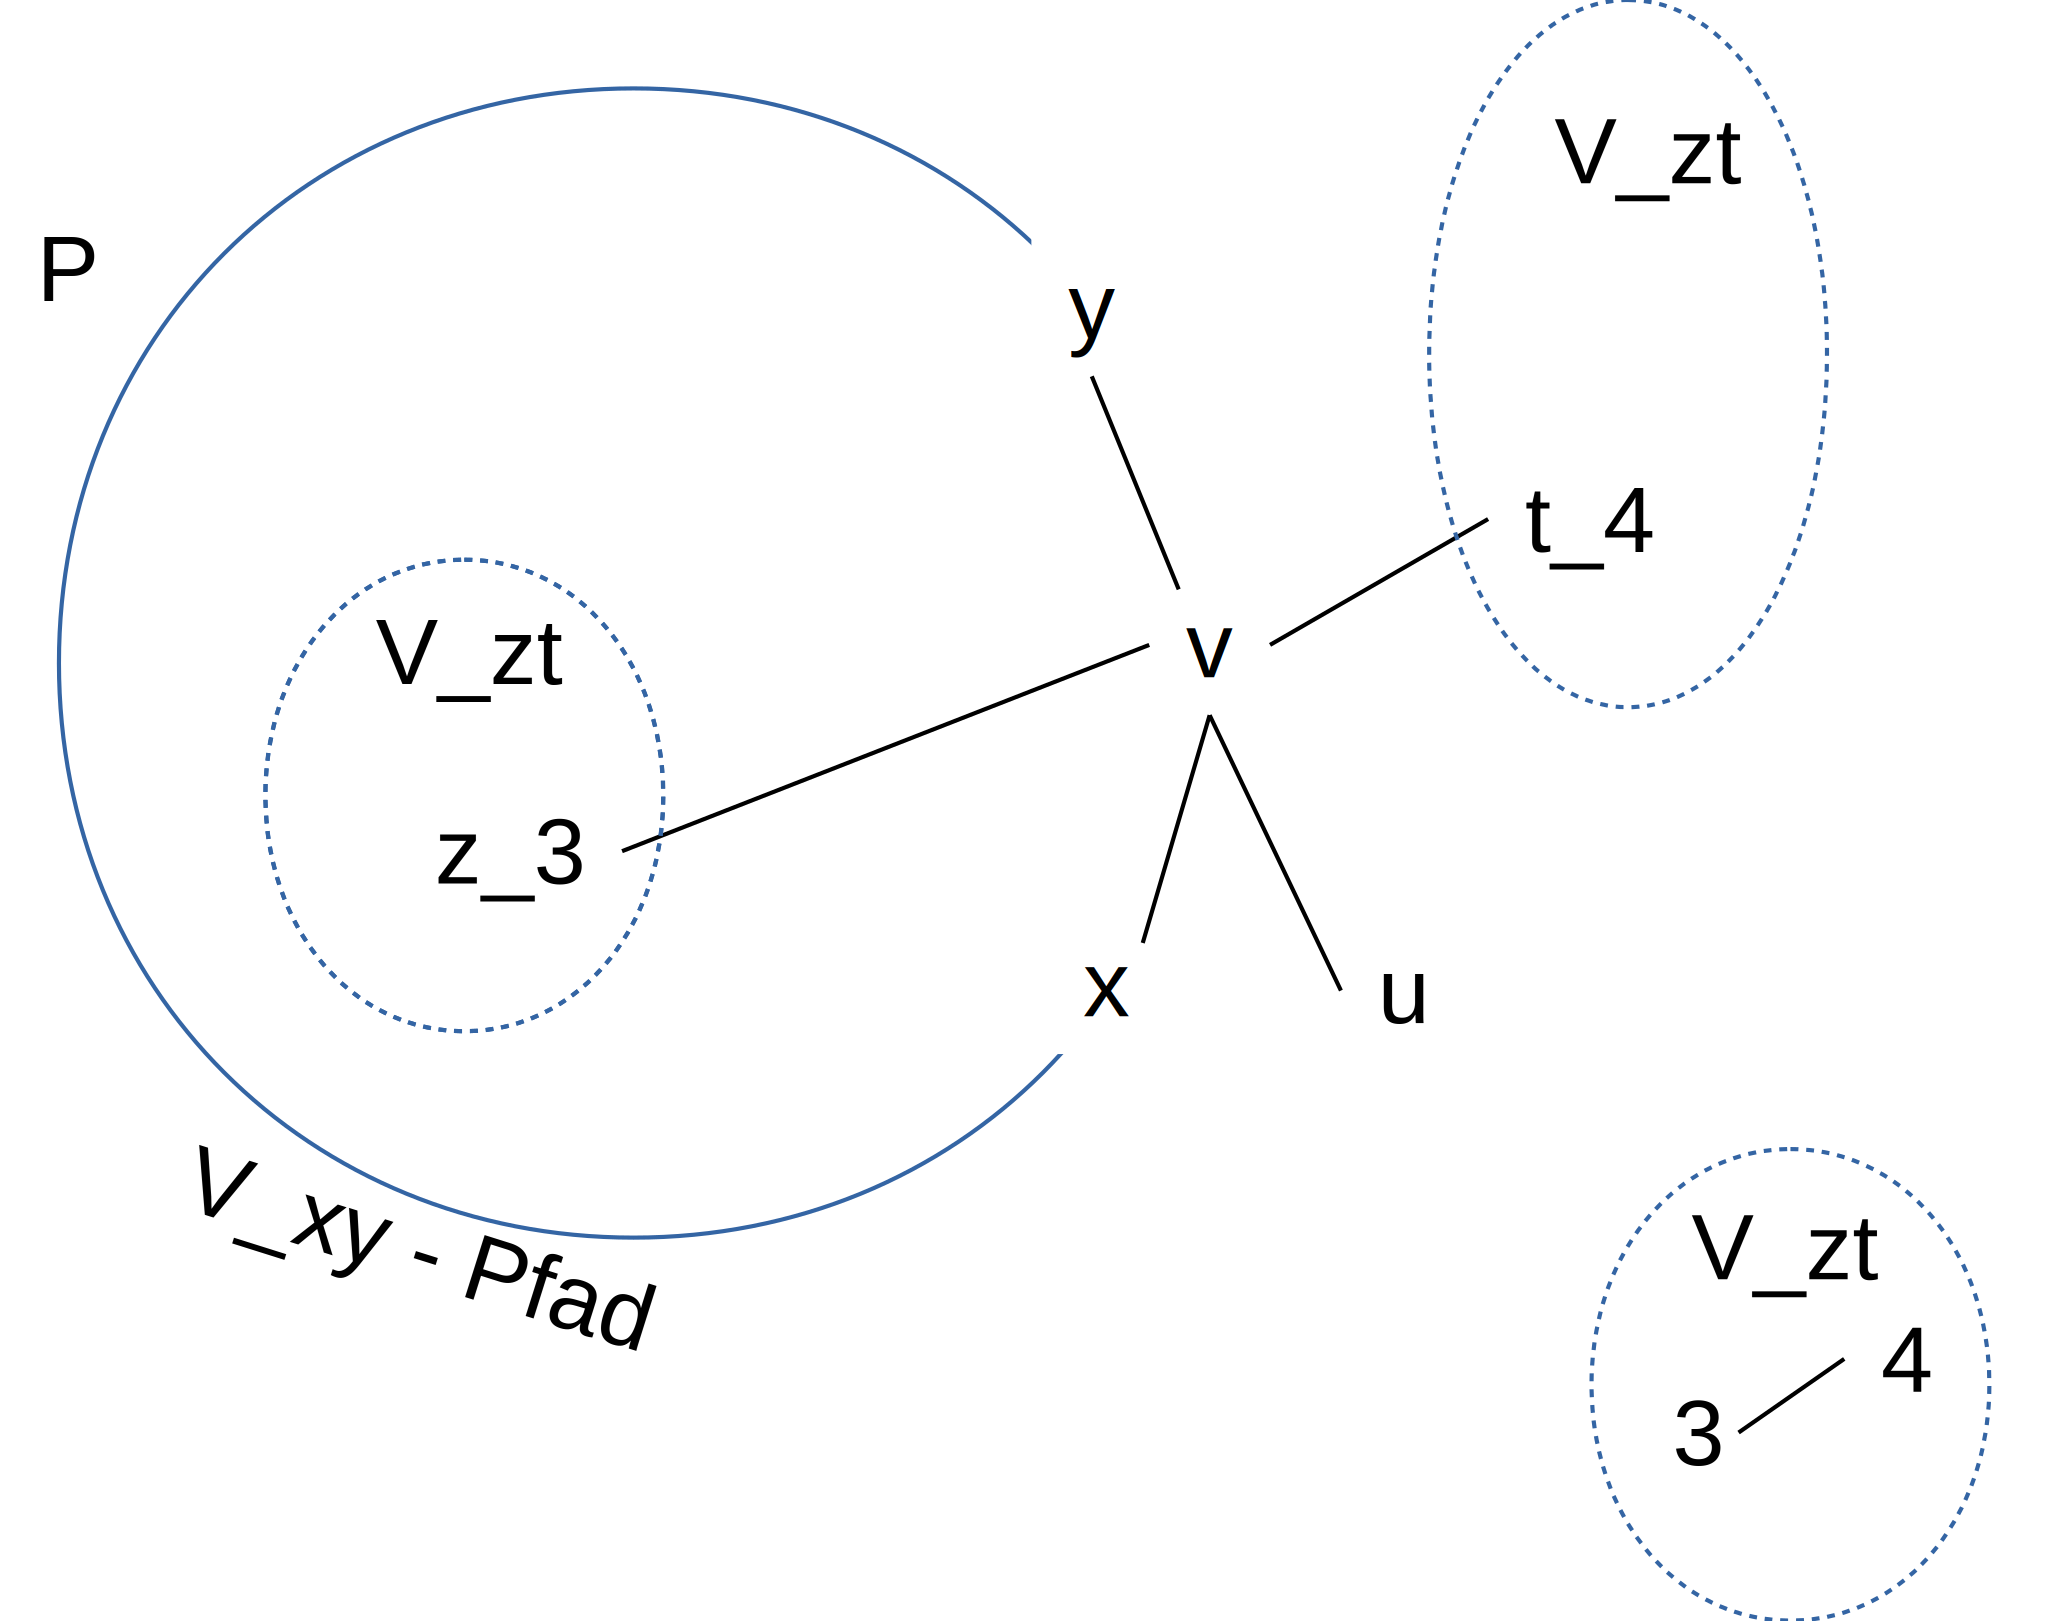
\includegraphics[scale=0.5]{lectures/161125/pix/3.pdf}
                                        \begin{itemize}
                                            \item $V_{zt}$: alle Knoten in $V(G \setminus \{v\})$, die $\mathcal{C}(t)$ oder $\mathcal{C}(z)$ gefärbt sind
                                            \item $V_{xy} \cap V_{zt} = \emptyset$!
                                            \item $V'_{zt}$ kann nur via eines $s \in P$ einen Knoten in $V_{zt} \setminus V'_{zt}$ erreichen
                                        \end{itemize}
                                        Damit lassen sich $z,t$ analog zu Fall (a) färben.
                                \end{enumerate}
                        \end{itemize}
                \end{enumerate}
        \end{description}
    \item[Theorem] Jeder planare Graph ist 4-färbbar
        \begin{description}
            \item[Proof] Es gibt eine Menge von 1936 4-färbbaren Karten, jede nicht Teil eines kleinsten Gegenbeispiels... (Appel, Haken, 1976).
            $\Rightarrow$ Es folgt, dass es kein kleinstes Gegenbeispiel gibt.
        \end{description}
\end{description}

\subsection{Zufallsgraphen}
Sei $G=(V,E)$ mit $V=\{1, \dots, n\}$ fixiert. Wir wollen nun Kanten zufällig auswählen auf dieser fixierten Kantenmenge $\{1, \dots, n\}$, um zufällige Graphen zu generieren. 
Die Menge dieser Zufallsgraphen nennen wir $\mathcal{G}$. \underline{Jede} Kante wird mit Wahrscheinlichkeit $p \in [0, \dots, 1]$ gewählt. 
Sei $G_0$ ein bestimmter Graph. Das Ereignis $\{G_0\}$ mit $G_0$ und m Kanten hat die Wahrscheinlichkeit $p^m \cdot (1-p)^{{n \over 2}-m}$. 
Wahrscheinlichkeitsmaß auf 
$\mathcal{G} ~ \forall e \in [v]^2$\\
$\Omega_e=\{0_e, 1_e\}$\\
$\mathbb{P}(\{1_e\})=p$\\
$\mathbb{P}(\{0_e\})=1-p$\\
$\Omega_\mathcal{G} = \prod\limits_{e \in [v]^2} \Omega_e$

\begin{description}
    \item[Beispiele] Fixiere Graph $H$, $V(H) = V(G)$, ist $H \leqslant G$? \\
        Mit $p^l$, $|E(H)| = l$, $|V(H)| = k$, aber falls $H$ induzierter Teilgraph von $G$ sein soll? \\
         - Nur $p^l (1-p)^{\binom{k}{2} - l}$. \\
        Und was ist mit Subgraph-Isomorphismus?
        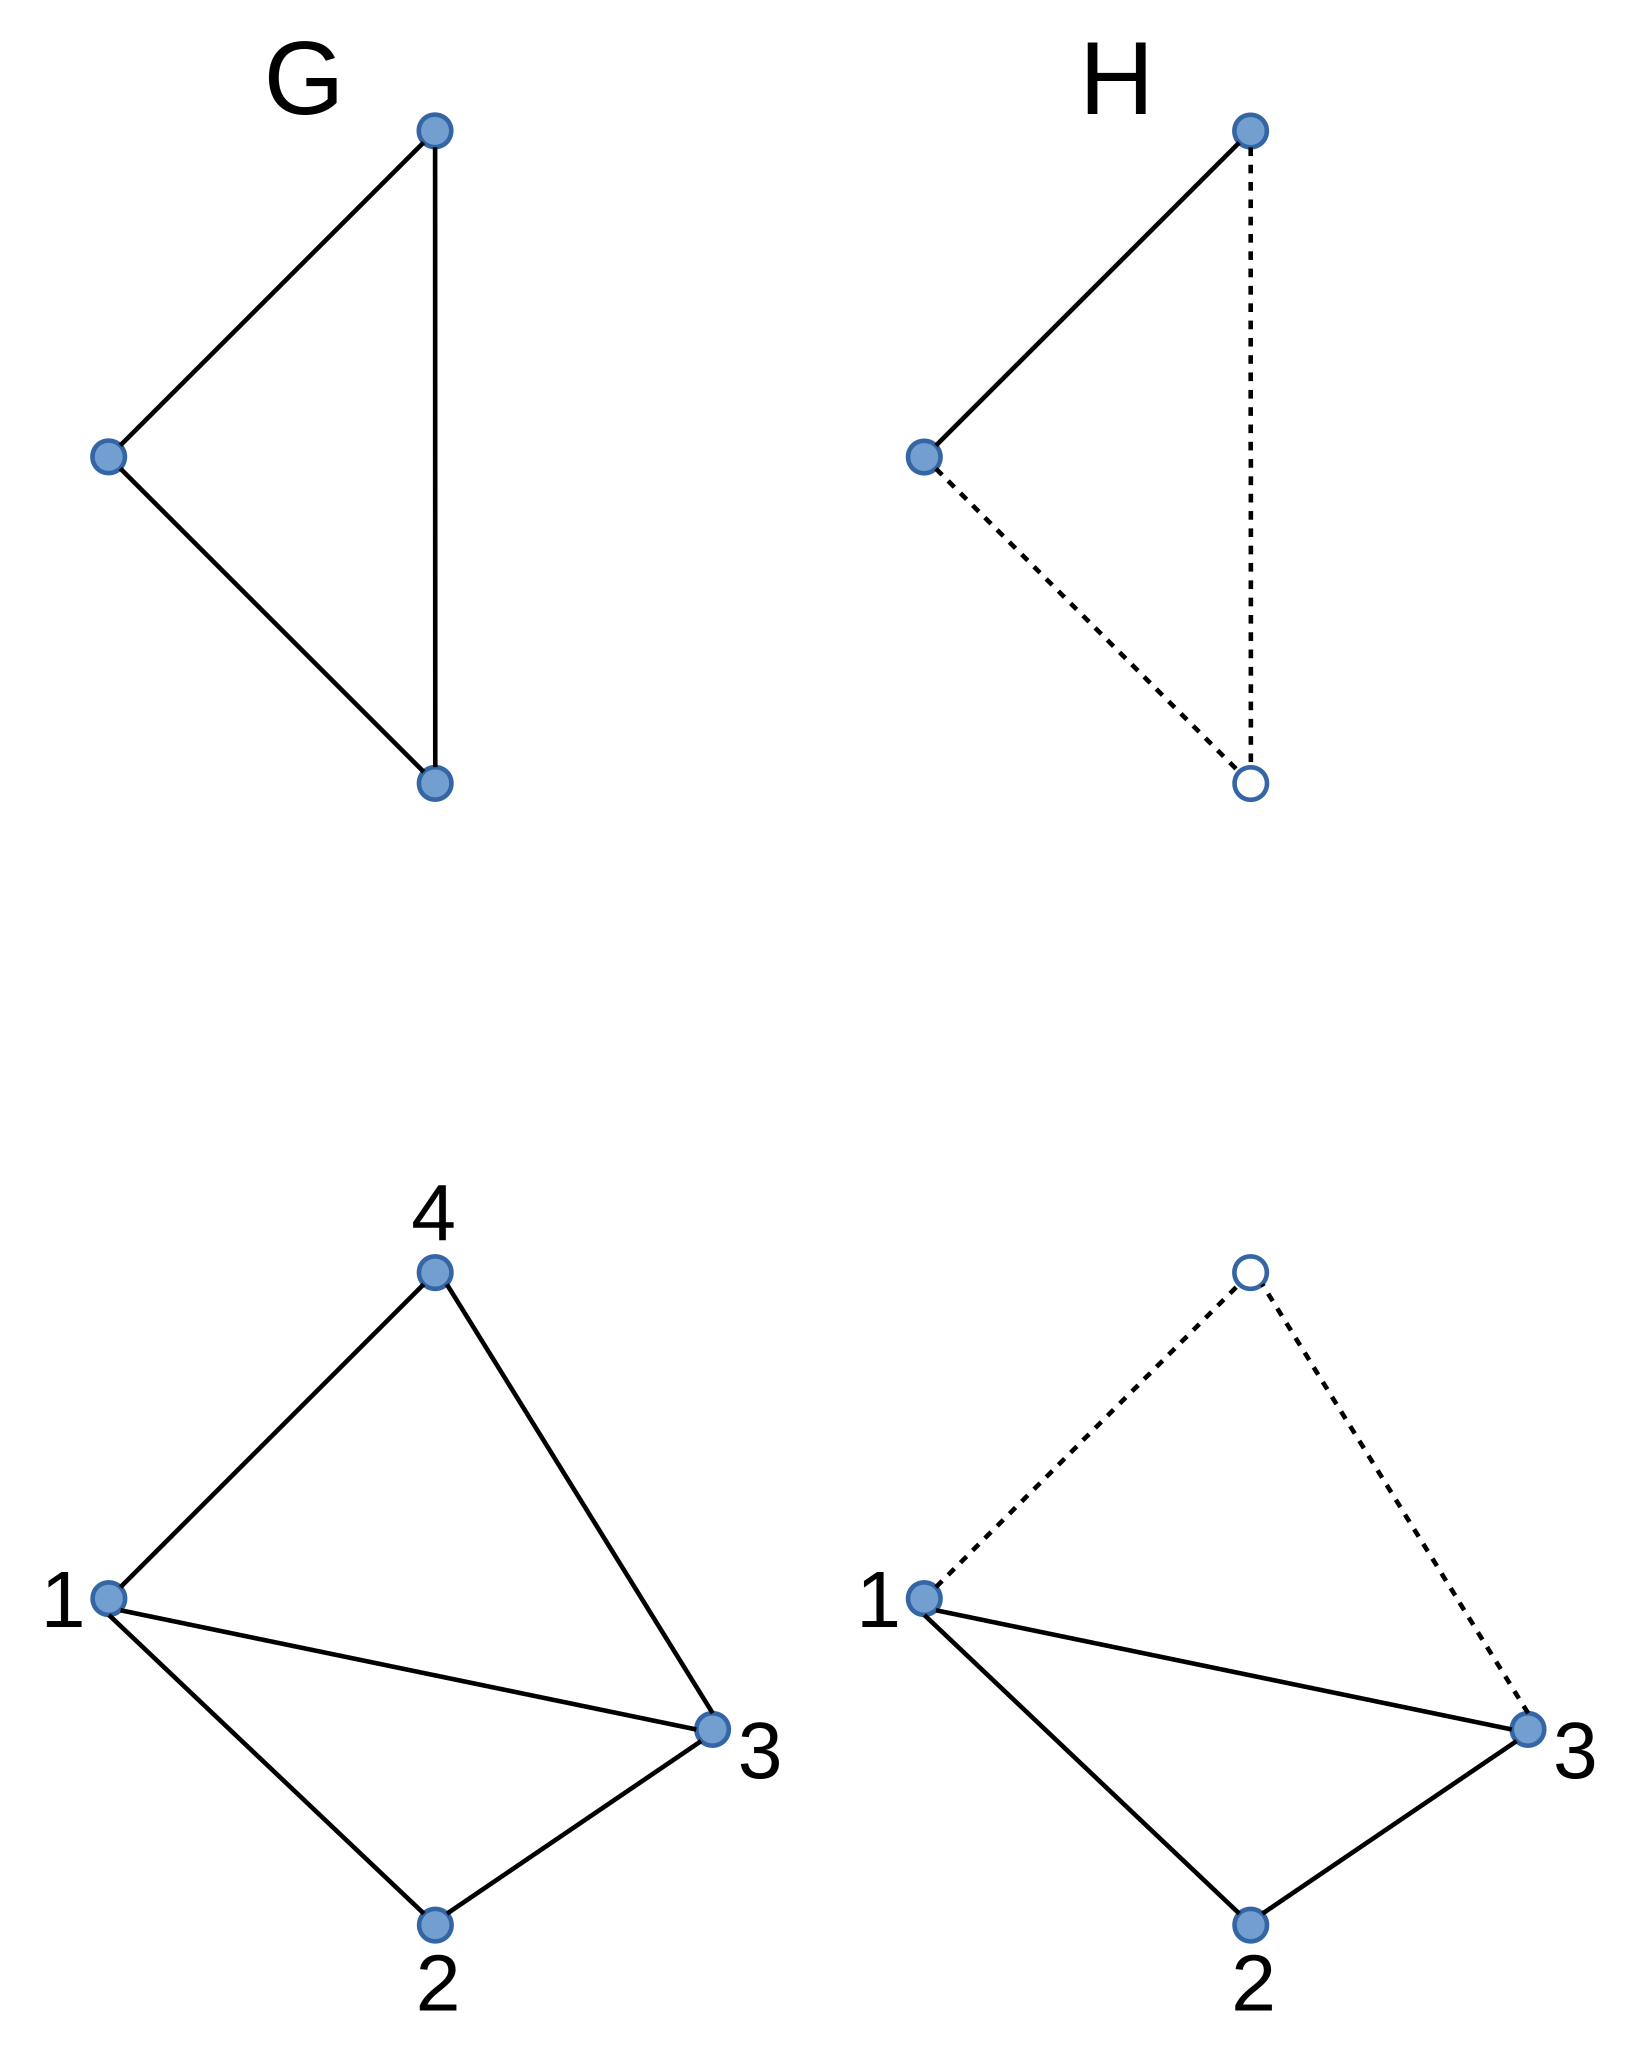
\includegraphics[scale=0.5]{lectures/161125/pix/4.pdf}
        \begin{itemize}
            \item Ereignismengen überlappen
            \item kompliziert
        \end{itemize}
\end{description}

\subsection{Eigenschaften fast aller Graphen}
Falls die Wahrscheinlichkeit, dass $P(G \in \mathcal{G}) \rightarrow 1$ für $n \rightarrow \infty$, dann geschieht $G$ fast sicher.
\begin{description}
    \item[Pro:] Gegeben jedes $H$ als Isomorphie-Klasse, $n \rightarrow \infty$ und $p \in ]0,1[ = (0,1)$, induzierte Kopie von $H$. 
    Dann haben fast alle $G$ in $\mathcal{G}(n,p)$ haben mindestens eine induzierte Kopie von $H$.
    \item[Prf:] Sei $H$ gegeben, $K=V(H)$. Sei $K \leqslant n$. $H$ ist (subgraph-) isomorph zu $G$ mit Wahrscheinlichkeit $r < 0$ ($G$ ist zufällig!). 
        Teile $G$ in $\lfloor {n \over k} \rfloor$ Teilgraphen, um genau so viele ``Versuche'' (für $r > 0$) zu haben. 
        $P(H \not \subseteq G$ induziert) $\leqslant (1-r)^{\lfloor {n \over k} \rfloor} \xrightarrow{n \rightarrow \infty} 0$
\end{description}


\newpage

\section{Vorlesung 25.11.2016}
\subsection{Färbung von Graphen}
\subsubsection{Vertexfärbung}
Zwei durch eine Kante verbundene Knoten haben unterschiedliche Farben.\\
Beispiel wäre eine Landkarte auf der mit so wenig wie möglich Farben die Länder ausgemalt werden, ohne zwei benachbarte Länder gleichfarbig zu haben. Hierbei entspricht jede Facette einen Knoten.\\
\includegraphics[width=0.4\textwidth]{lectures/161125/pix/Vertexfaerbung}
\begin{description}
    \item[Vertexfärbung] Eine Vertexfärbung eines Graphen $G=(V,E)$ ist eine Abbildung $\mathcal{C} \colon V \mapsto \mathcal{S}$, mit $\mathcal{S}=$ Menge der Farben. Es gilt, dass $\mathcal{C}(v) \neq \mathcal{C}(w)$, mit $w,v \in \mathcal{S}$, wenn $v$ und $w$ adjazent ($\{v,w\} \in E$) sind. Die Elemente von $\mathcal{S}$ heißen \emph{Farben}.
    \item[k-Färbung] Ein Graph $G$ ist $k$-färbbar, wenn es für eine Abbildung $\mathcal{C}$ eine Menge $\mathcal{S}=\{1,\dots,k\}$ gibt.
    \item[Chromatische Zahl] Eine chromatische Zahl $\chi(G)$ ist die kleinste natürliche Zahl $k$, sodass G $k$-färbbar ist. $\chi(G) \leqslant \Delta(G) + 1$, mit $\Delta(G) = $ maximaler Grad von $G$
        \begin{description}
            \item[Proof (greedy)] Färbe $v_i$ der Vertices $v_1 \dots v_n$ mit der kleinsten Farbe, die nicht von einem Nachbarn von $v_i$ benutzt wird. Da wir max. $\Delta(G)$ viele Nachbarn für $v_i$ haben, gibt es immer eine freie Farbe.
        \end{description}
        $\chi(G) \geqslant$ Größe der größten Clique
    \item[Lemma] Für jeden einfachen planaren Graphen $G$ ist der Durchschnittsgrad $d(G) < 6$
        \begin{description}
            \item[Proof] $d(G) = 2 \cdot {|E| \over |V|}$ mit $|V| \leqslant 3$, $|E| \leqslant 3  \cdot |V| - 6$, dann $d(G) \leqslant {2(3 \cdot |V|-6) \over |V|} = 6-{12 \over |V|}$
        \end{description}
    \item[Theorem] Jeder simple planare Graph $G$ hat $\chi(G) \leqslant 6$
        \begin{description}
            \item[Proof] Annahme: Jeder simple planare Graph mit $|V| = n$ ist $6$-färbbar.
            \begin{itemize}
                \item Sei $G$ hiermit ein simpler planarer Graph mit $|V| = n+1$
                \item Vom Lemma wissen wir, dass $w \in V$ mit $d(w) \leqslant 5$ existiert
                \item Sei $G' = G \setminus \{w\}$. Via Induktionshypothese ist $G'$ 6-färbbar. Das tun wir dann.
                \item Färbe $w$ mit der (min.) freien Farbe, um $G$ zu färben
            \end{itemize}
        \end{description}
    \item[Theorem] Für jeden simplen planaren Graphen $G$ gilt, dass $\chi(G) \leqslant 5$
        \begin{description}
            \item[Proof] Sei $G=(V,E)$ planar
                \begin{enumerate}
                    \item Falls $|V| \leqslant 5 \rightarrow$ trivial
                    \item Für alle $v \in V(G)$ mit $deg(v) < 5$, färbe $v$ und arbeite mit $G \setminus \{v\}$
                    \item $G$ hat Vertex $v$ mit $deg(v) = 5$
                        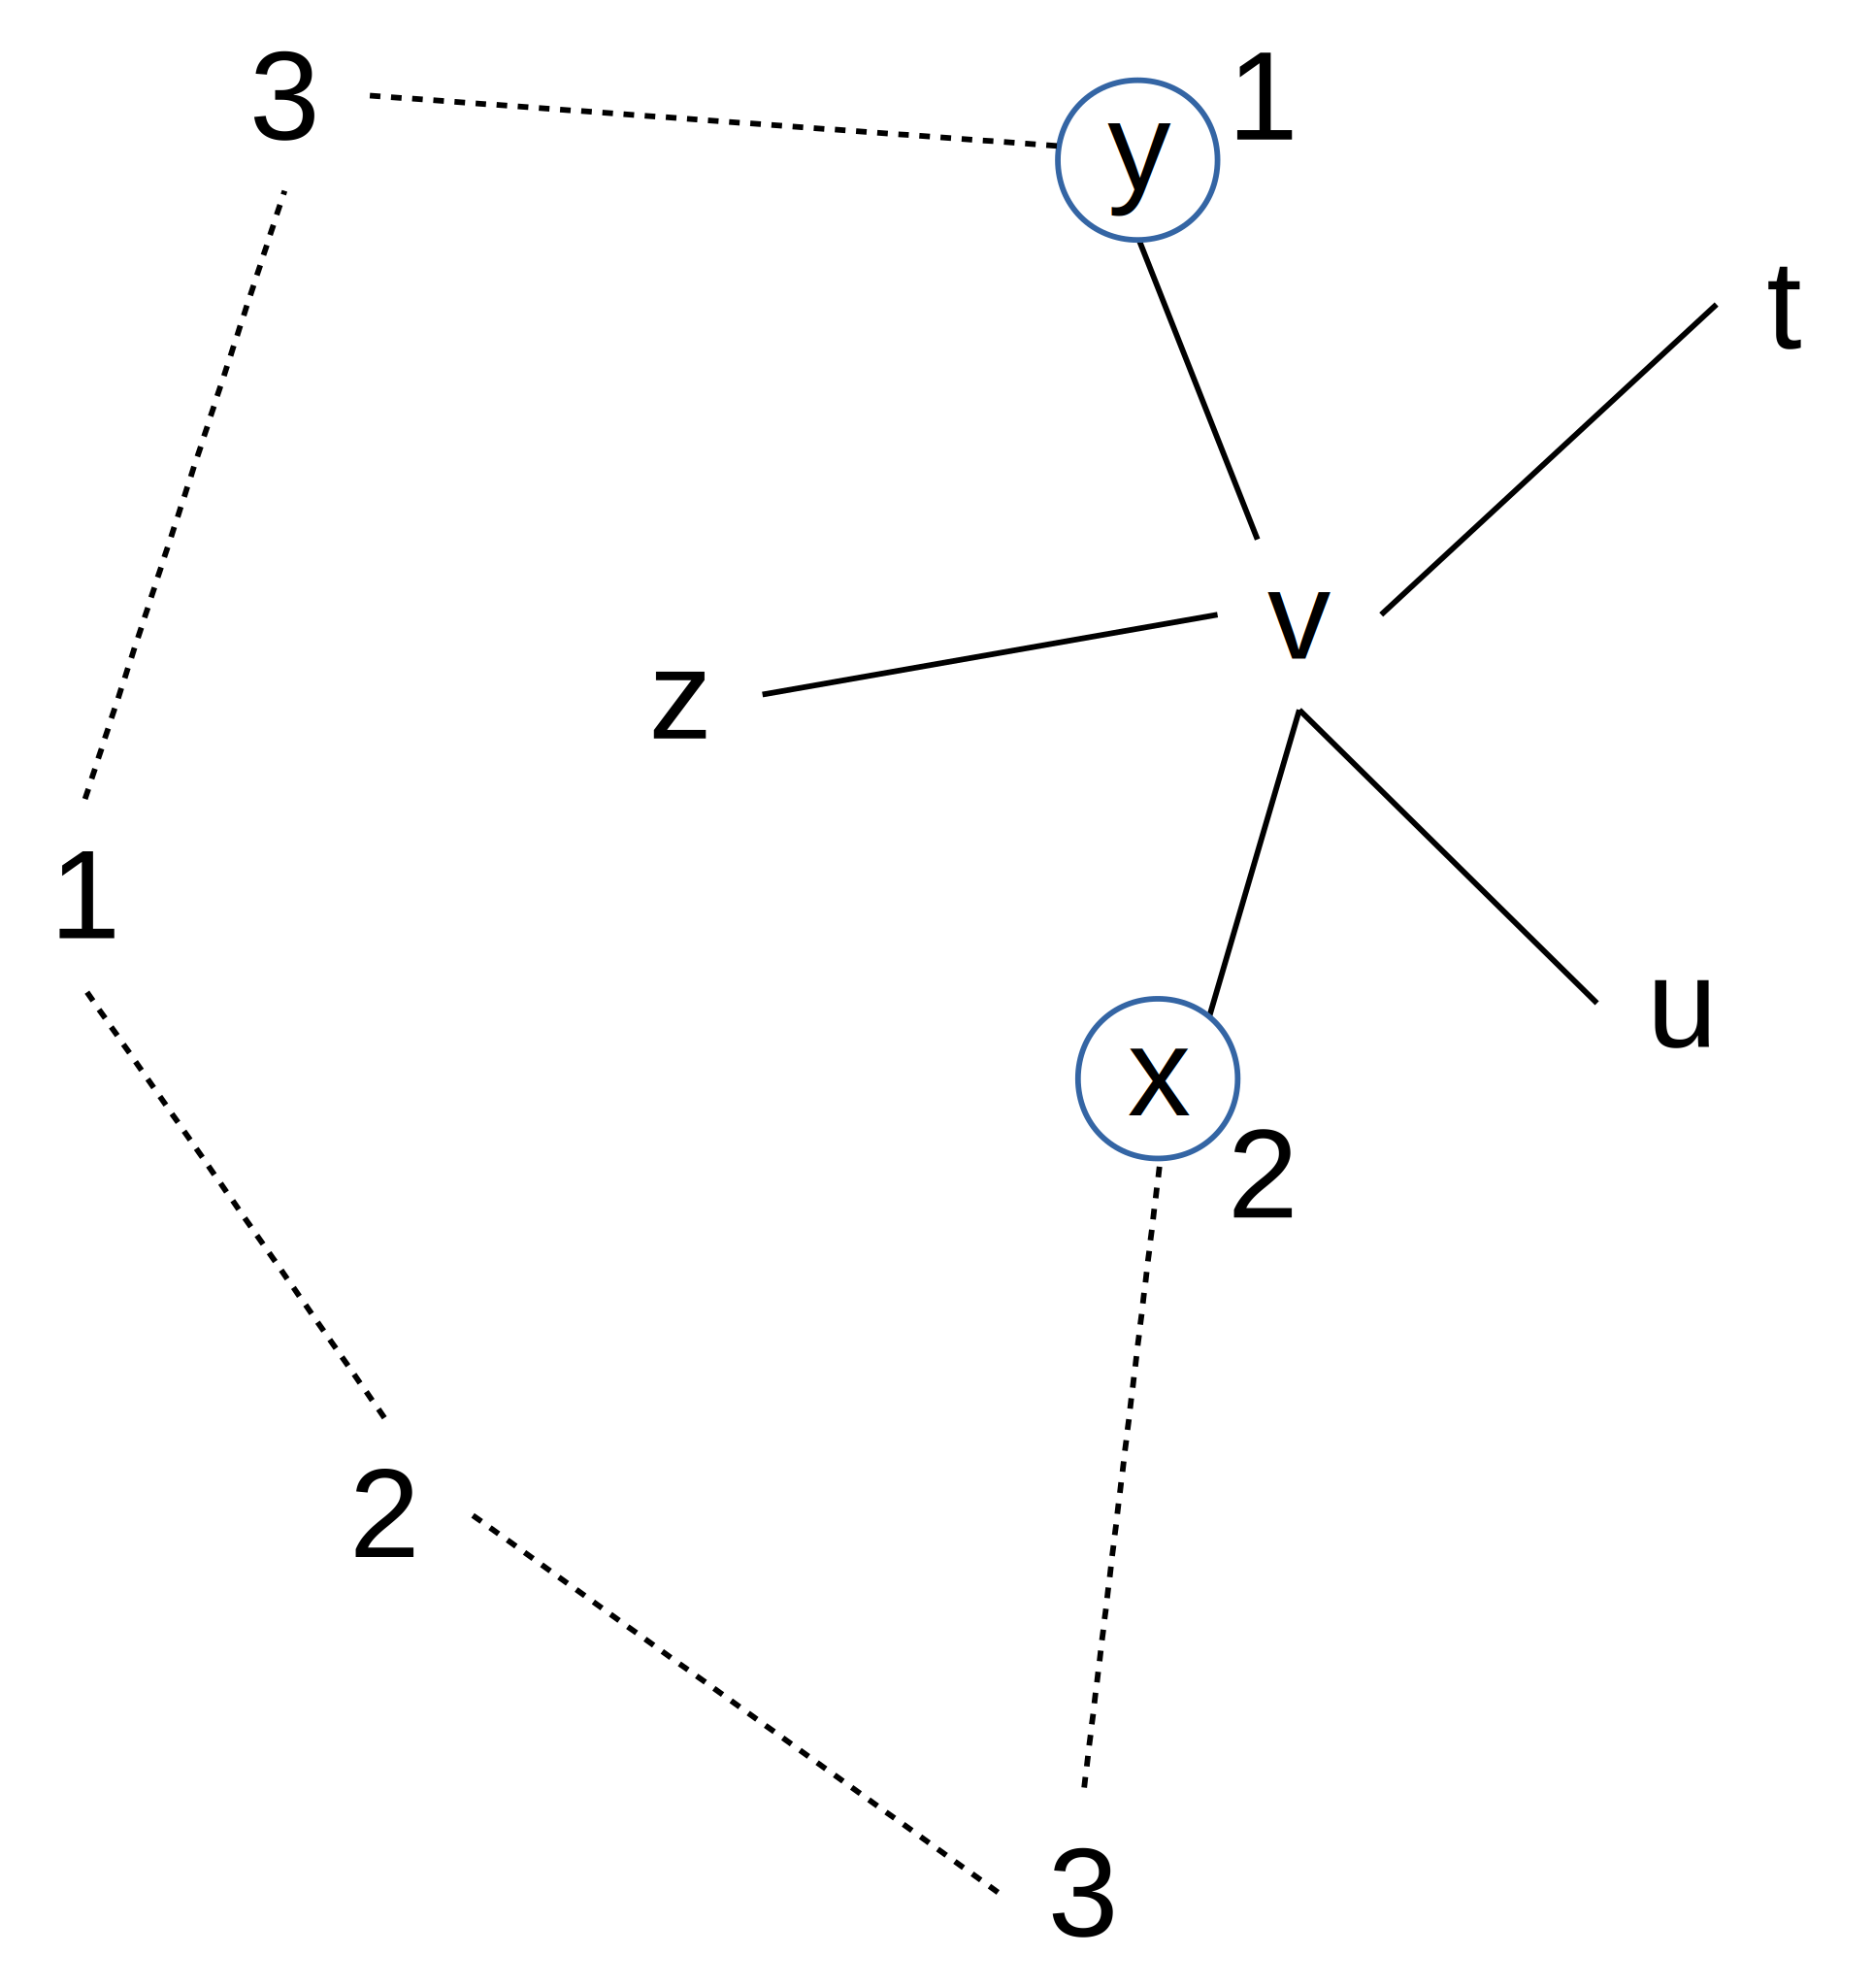
\includegraphics[scale=0.5]{lectures/161125/pix/2.pdf}
                        \begin{itemize}
                            \item betrachte 5-Färbung $\mathcal{C} \colon V(G \setminus \{v\}) \mapsto \{1, \dots, 5\}$, die es nach Rekursion gibt
                            \item betrache $x,y \in V_{xy}$ und sei $V_{xy} \subset V(G)$ die Menge der Knoten mit $\mathcal{C}(x)$- oder $\mathcal{C}(y)$-Färbung
                                \begin{enumerate}
                                    \item es gibt \underline{keinen} Weg von $x \rightsquigarrow y$, der nur Knoten aus $V_{xy}$ nutzt
                                        \begin{itemize}
                                            \item Seien $V'_{xy}$ die $s \in V(G \setminus \{v\})$, die von $x$ nur via $V_{xy}$ erreicht werden
                                            \item Färbe um:
                                            \begin{math}
                                                \mathcal{C'}(s) =
                                                    \begin{cases}
                                                        \mathcal{C}(s) & s \not \in V'_{xy}\\
                                                        \mathcal{C}(y) & s \in V'_{xy}, ~ \mathcal{C}(s) = \mathcal{C}(x)\\
                                                        \mathcal{C}(x) & s \in V'_{xy}, ~ \mathcal{C}(s) = \mathcal{C}(y)
                                                    \end{cases}
                                            \end{math}\\\\
                                            ``Tausche Farben auf $V'_{xy}$'' $\Rightarrow \mathcal{C'}(x) = \mathcal{C'}(y) = \mathcal{C}(y)$
                                        \end{itemize}
                                    \item es gibt einen solchen Pfad $x \rightsquigarrow y$ mit allen Knoten in $V_{xy}$
                                    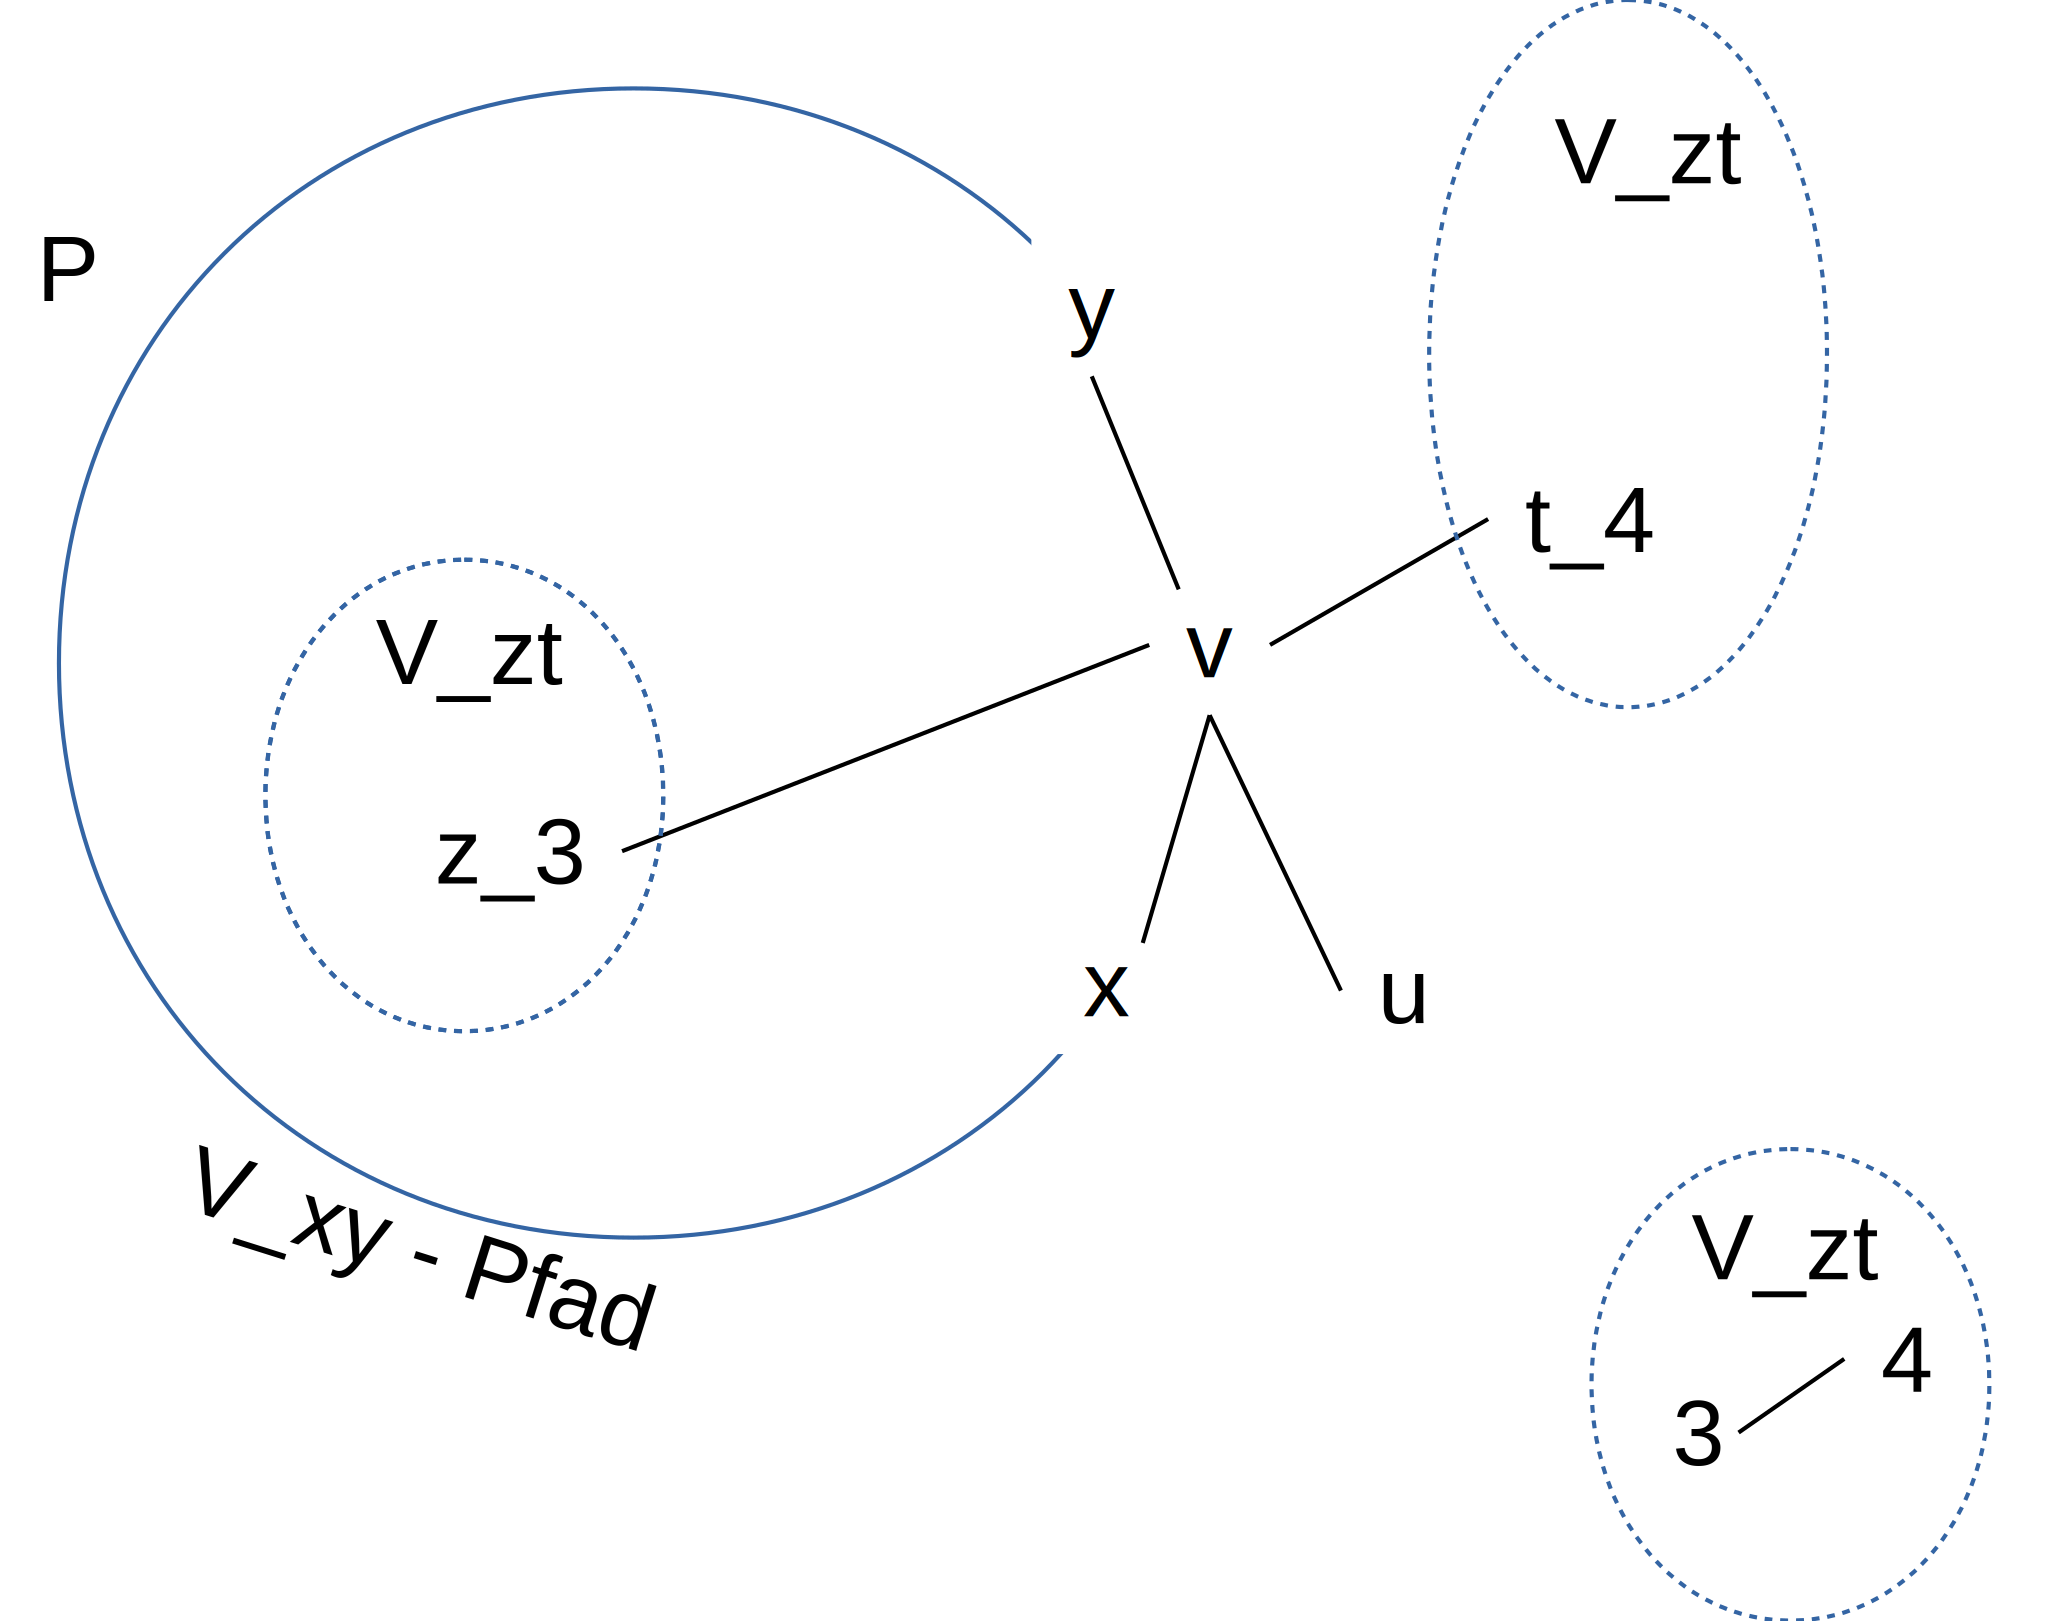
\includegraphics[scale=0.5]{lectures/161125/pix/3.pdf}
                                        \begin{itemize}
                                            \item $V_{zt}$: alle Knoten in $V(G \setminus \{v\})$, die $\mathcal{C}(t)$ oder $\mathcal{C}(z)$ gefärbt sind
                                            \item $V_{xy} \cap V_{zt} = \emptyset$!
                                            \item $V'_{zt}$ kann nur via eines $s \in P$ einen Knoten in $V_{zt} \setminus V'_{zt}$ erreichen
                                        \end{itemize}
                                        Damit lassen sich $z,t$ analog zu Fall (a) färben.
                                \end{enumerate}
                        \end{itemize}
                \end{enumerate}
        \end{description}
    \item[Theorem] Jeder planare Graph ist 4-färbbar
        \begin{description}
            \item[Proof] Es gibt eine Menge von 1936 4-färbbaren Karten, jede nicht Teil eines kleinsten Gegenbeispiels... (Appel, Haken, 1976).
            $\Rightarrow$ Es folgt, dass es kein kleinstes Gegenbeispiel gibt.
        \end{description}
\end{description}

\subsection{Zufallsgraphen}
Sei $G=(V,E)$ mit $V=\{1, \dots, n\}$ fixiert. Wir wollen nun Kanten zufällig auswählen auf dieser fixierten Kantenmenge $\{1, \dots, n\}$, um zufällige Graphen zu generieren. 
Die Menge dieser Zufallsgraphen nennen wir $\mathcal{G}$. \underline{Jede} Kante wird mit Wahrscheinlichkeit $p \in [0, \dots, 1]$ gewählt. 
Sei $G_0$ ein bestimmter Graph. Das Ereignis $\{G_0\}$ mit $G_0$ und m Kanten hat die Wahrscheinlichkeit $p^m \cdot (1-p)^{{n \over 2}-m}$. 
Wahrscheinlichkeitsmaß auf 
$\mathcal{G} ~ \forall e \in [v]^2$\\
$\Omega_e=\{0_e, 1_e\}$\\
$\mathbb{P}(\{1_e\})=p$\\
$\mathbb{P}(\{0_e\})=1-p$\\
$\Omega_\mathcal{G} = \prod\limits_{e \in [v]^2} \Omega_e$

\begin{description}
    \item[Beispiele] Fixiere Graph $H$, $V(H) = V(G)$, ist $H \leqslant G$? \\
        Mit $p^l$, $|E(H)| = l$, $|V(H)| = k$, aber falls $H$ induzierter Teilgraph von $G$ sein soll? \\
         - Nur $p^l (1-p)^{\binom{k}{2} - l}$. \\
        Und was ist mit Subgraph-Isomorphismus?
        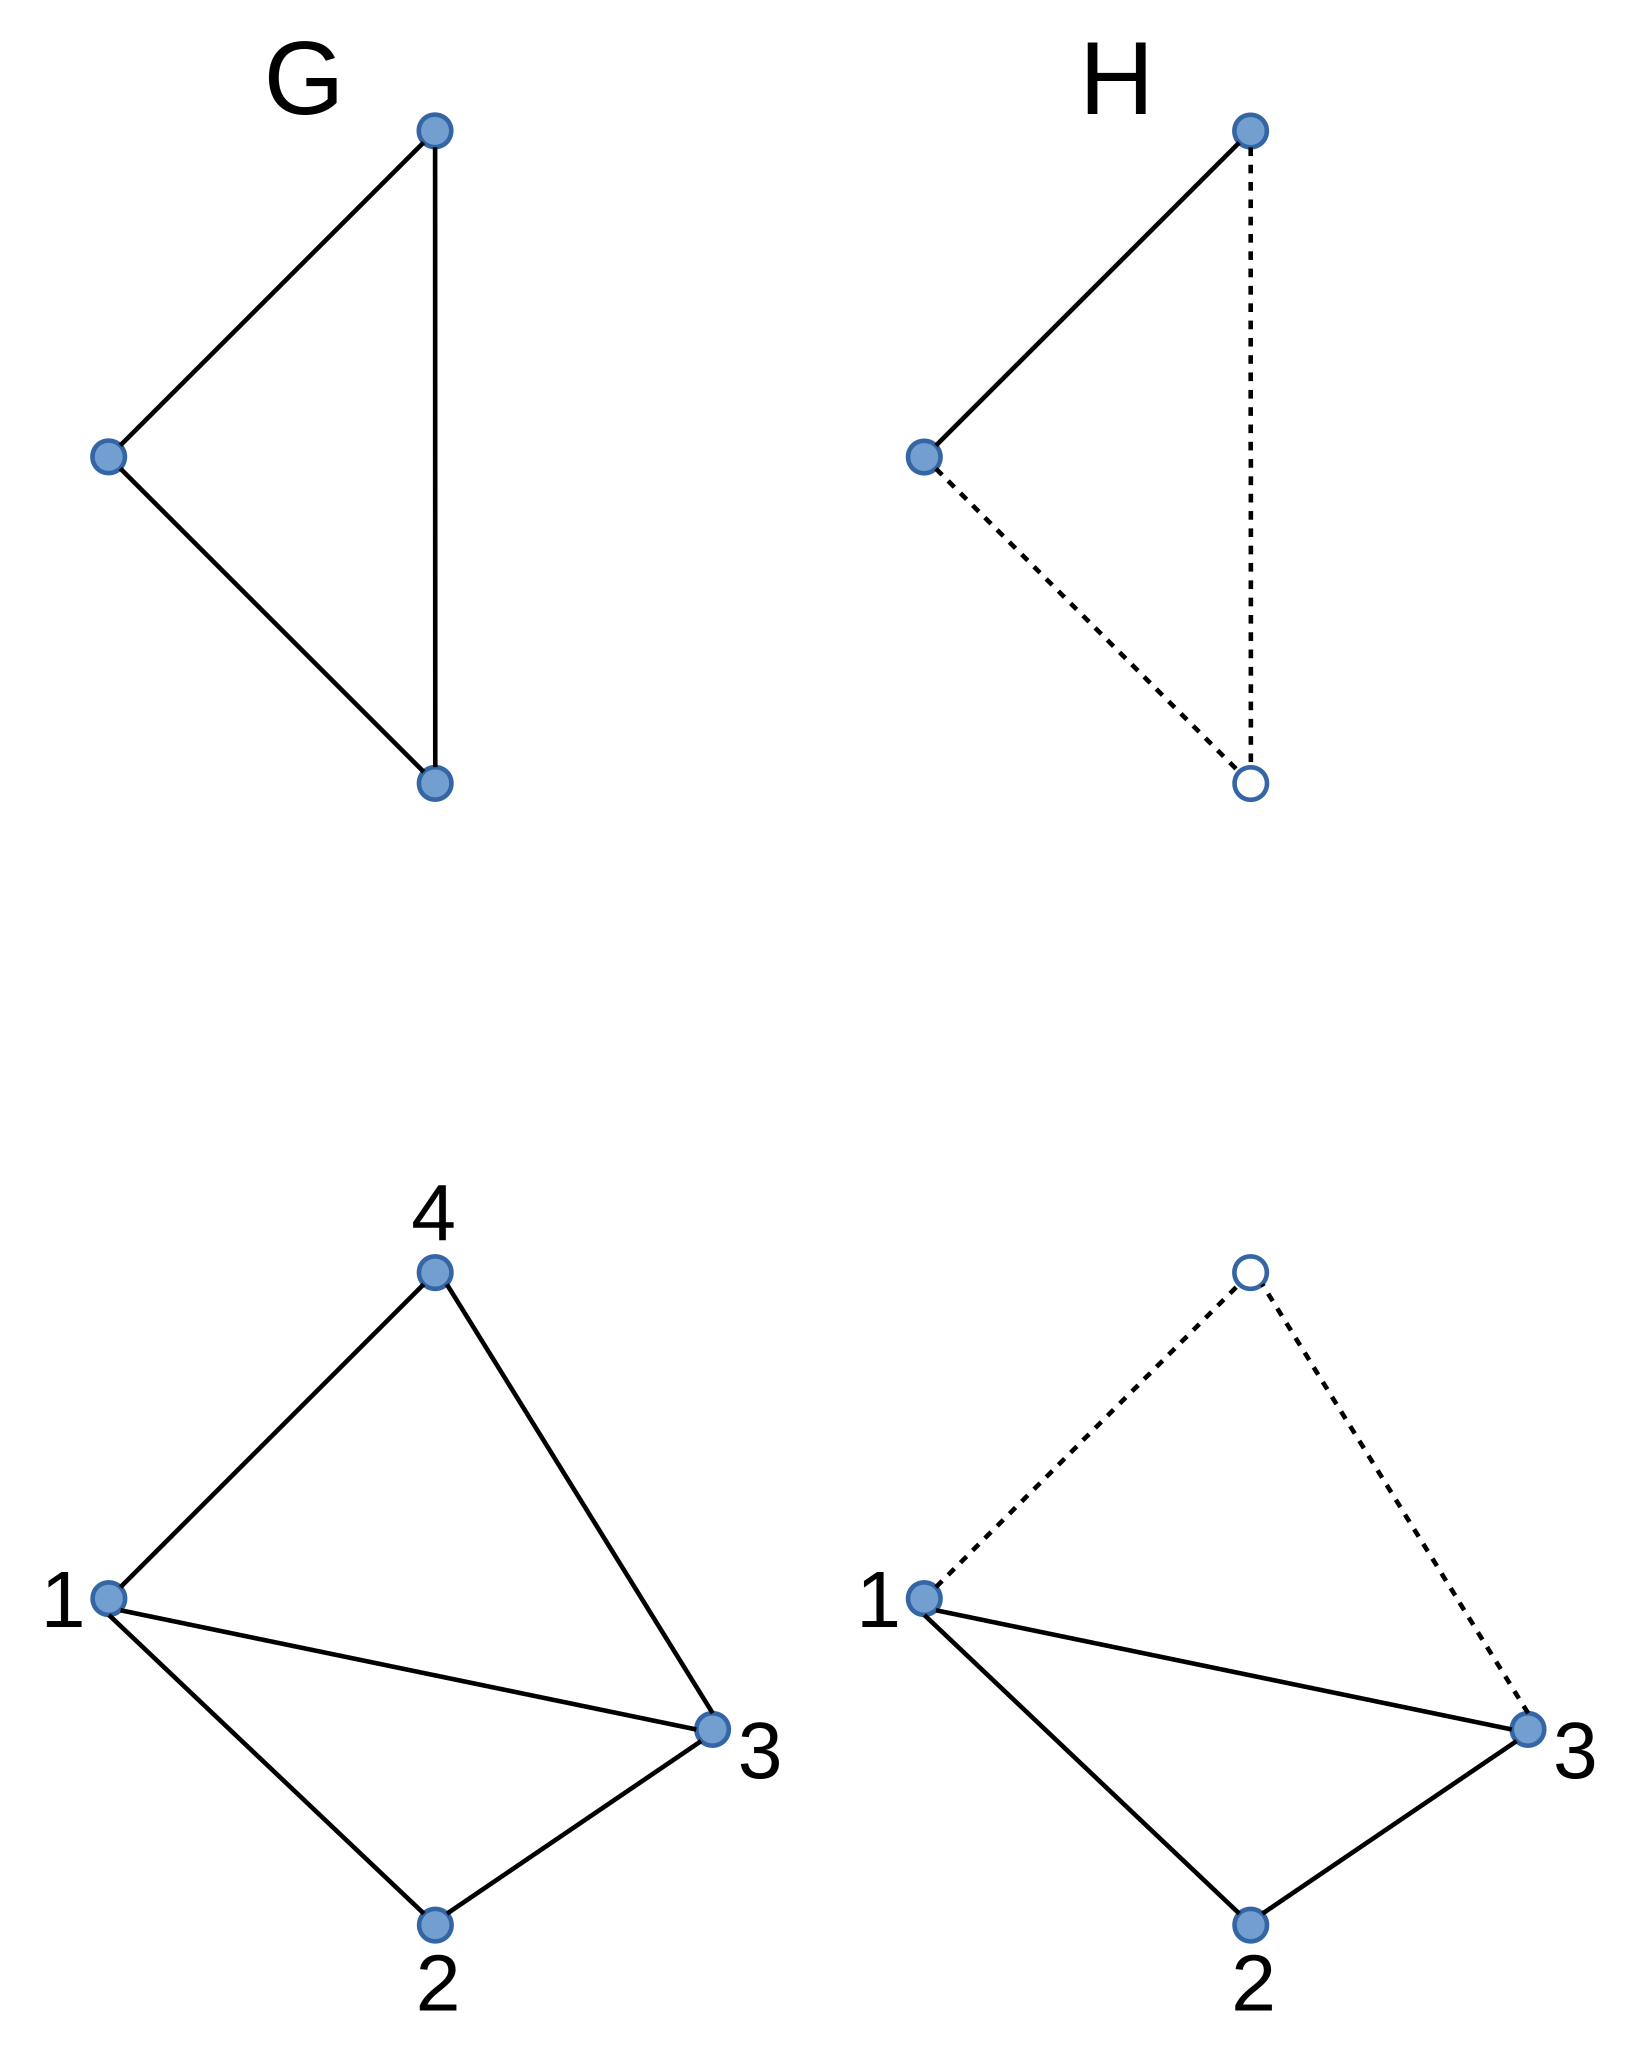
\includegraphics[scale=0.5]{lectures/161125/pix/4.pdf}
        \begin{itemize}
            \item Ereignismengen überlappen
            \item kompliziert
        \end{itemize}
\end{description}

\subsection{Eigenschaften fast aller Graphen}
Falls die Wahrscheinlichkeit, dass $P(G \in \mathcal{G}) \rightarrow 1$ für $n \rightarrow \infty$, dann geschieht $G$ fast sicher.
\begin{description}
    \item[Pro:] Gegeben jedes $H$ als Isomorphie-Klasse, $n \rightarrow \infty$ und $p \in ]0,1[ = (0,1)$, induzierte Kopie von $H$. 
    Dann haben fast alle $G$ in $\mathcal{G}(n,p)$ haben mindestens eine induzierte Kopie von $H$.
    \item[Prf:] Sei $H$ gegeben, $K=V(H)$. Sei $K \leqslant n$. $H$ ist (subgraph-) isomorph zu $G$ mit Wahrscheinlichkeit $r < 0$ ($G$ ist zufällig!). 
        Teile $G$ in $\lfloor {n \over k} \rfloor$ Teilgraphen, um genau so viele ``Versuche'' (für $r > 0$) zu haben. 
        $P(H \not \subseteq G$ induziert) $\leqslant (1-r)^{\lfloor {n \over k} \rfloor} \xrightarrow{n \rightarrow \infty} 0$
\end{description}


\newpage

\section{Vorlesung 25.11.2016}
\subsection{Färbung von Graphen}
\subsubsection{Vertexfärbung}
Zwei durch eine Kante verbundene Knoten haben unterschiedliche Farben.\\
Beispiel wäre eine Landkarte auf der mit so wenig wie möglich Farben die Länder ausgemalt werden, ohne zwei benachbarte Länder gleichfarbig zu haben. Hierbei entspricht jede Facette einen Knoten.\\
\includegraphics[width=0.4\textwidth]{lectures/161125/pix/Vertexfaerbung}
\begin{description}
    \item[Vertexfärbung] Eine Vertexfärbung eines Graphen $G=(V,E)$ ist eine Abbildung $\mathcal{C} \colon V \mapsto \mathcal{S}$, mit $\mathcal{S}=$ Menge der Farben. Es gilt, dass $\mathcal{C}(v) \neq \mathcal{C}(w)$, mit $w,v \in \mathcal{S}$, wenn $v$ und $w$ adjazent ($\{v,w\} \in E$) sind. Die Elemente von $\mathcal{S}$ heißen \emph{Farben}.
    \item[k-Färbung] Ein Graph $G$ ist $k$-färbbar, wenn es für eine Abbildung $\mathcal{C}$ eine Menge $\mathcal{S}=\{1,\dots,k\}$ gibt.
    \item[Chromatische Zahl] Eine chromatische Zahl $\chi(G)$ ist die kleinste natürliche Zahl $k$, sodass G $k$-färbbar ist. $\chi(G) \leqslant \Delta(G) + 1$, mit $\Delta(G) = $ maximaler Grad von $G$
        \begin{description}
            \item[Proof (greedy)] Färbe $v_i$ der Vertices $v_1 \dots v_n$ mit der kleinsten Farbe, die nicht von einem Nachbarn von $v_i$ benutzt wird. Da wir max. $\Delta(G)$ viele Nachbarn für $v_i$ haben, gibt es immer eine freie Farbe.
        \end{description}
        $\chi(G) \geqslant$ Größe der größten Clique
    \item[Lemma] Für jeden einfachen planaren Graphen $G$ ist der Durchschnittsgrad $d(G) < 6$
        \begin{description}
            \item[Proof] $d(G) = 2 \cdot {|E| \over |V|}$ mit $|V| \leqslant 3$, $|E| \leqslant 3  \cdot |V| - 6$, dann $d(G) \leqslant {2(3 \cdot |V|-6) \over |V|} = 6-{12 \over |V|}$
        \end{description}
    \item[Theorem] Jeder simple planare Graph $G$ hat $\chi(G) \leqslant 6$
        \begin{description}
            \item[Proof] Annahme: Jeder simple planare Graph mit $|V| = n$ ist $6$-färbbar.
            \begin{itemize}
                \item Sei $G$ hiermit ein simpler planarer Graph mit $|V| = n+1$
                \item Vom Lemma wissen wir, dass $w \in V$ mit $d(w) \leqslant 5$ existiert
                \item Sei $G' = G \setminus \{w\}$. Via Induktionshypothese ist $G'$ 6-färbbar. Das tun wir dann.
                \item Färbe $w$ mit der (min.) freien Farbe, um $G$ zu färben
            \end{itemize}
        \end{description}
    \item[Theorem] Für jeden simplen planaren Graphen $G$ gilt, dass $\chi(G) \leqslant 5$
        \begin{description}
            \item[Proof] Sei $G=(V,E)$ planar
                \begin{enumerate}
                    \item Falls $|V| \leqslant 5 \rightarrow$ trivial
                    \item Für alle $v \in V(G)$ mit $deg(v) < 5$, färbe $v$ und arbeite mit $G \setminus \{v\}$
                    \item $G$ hat Vertex $v$ mit $deg(v) = 5$
                        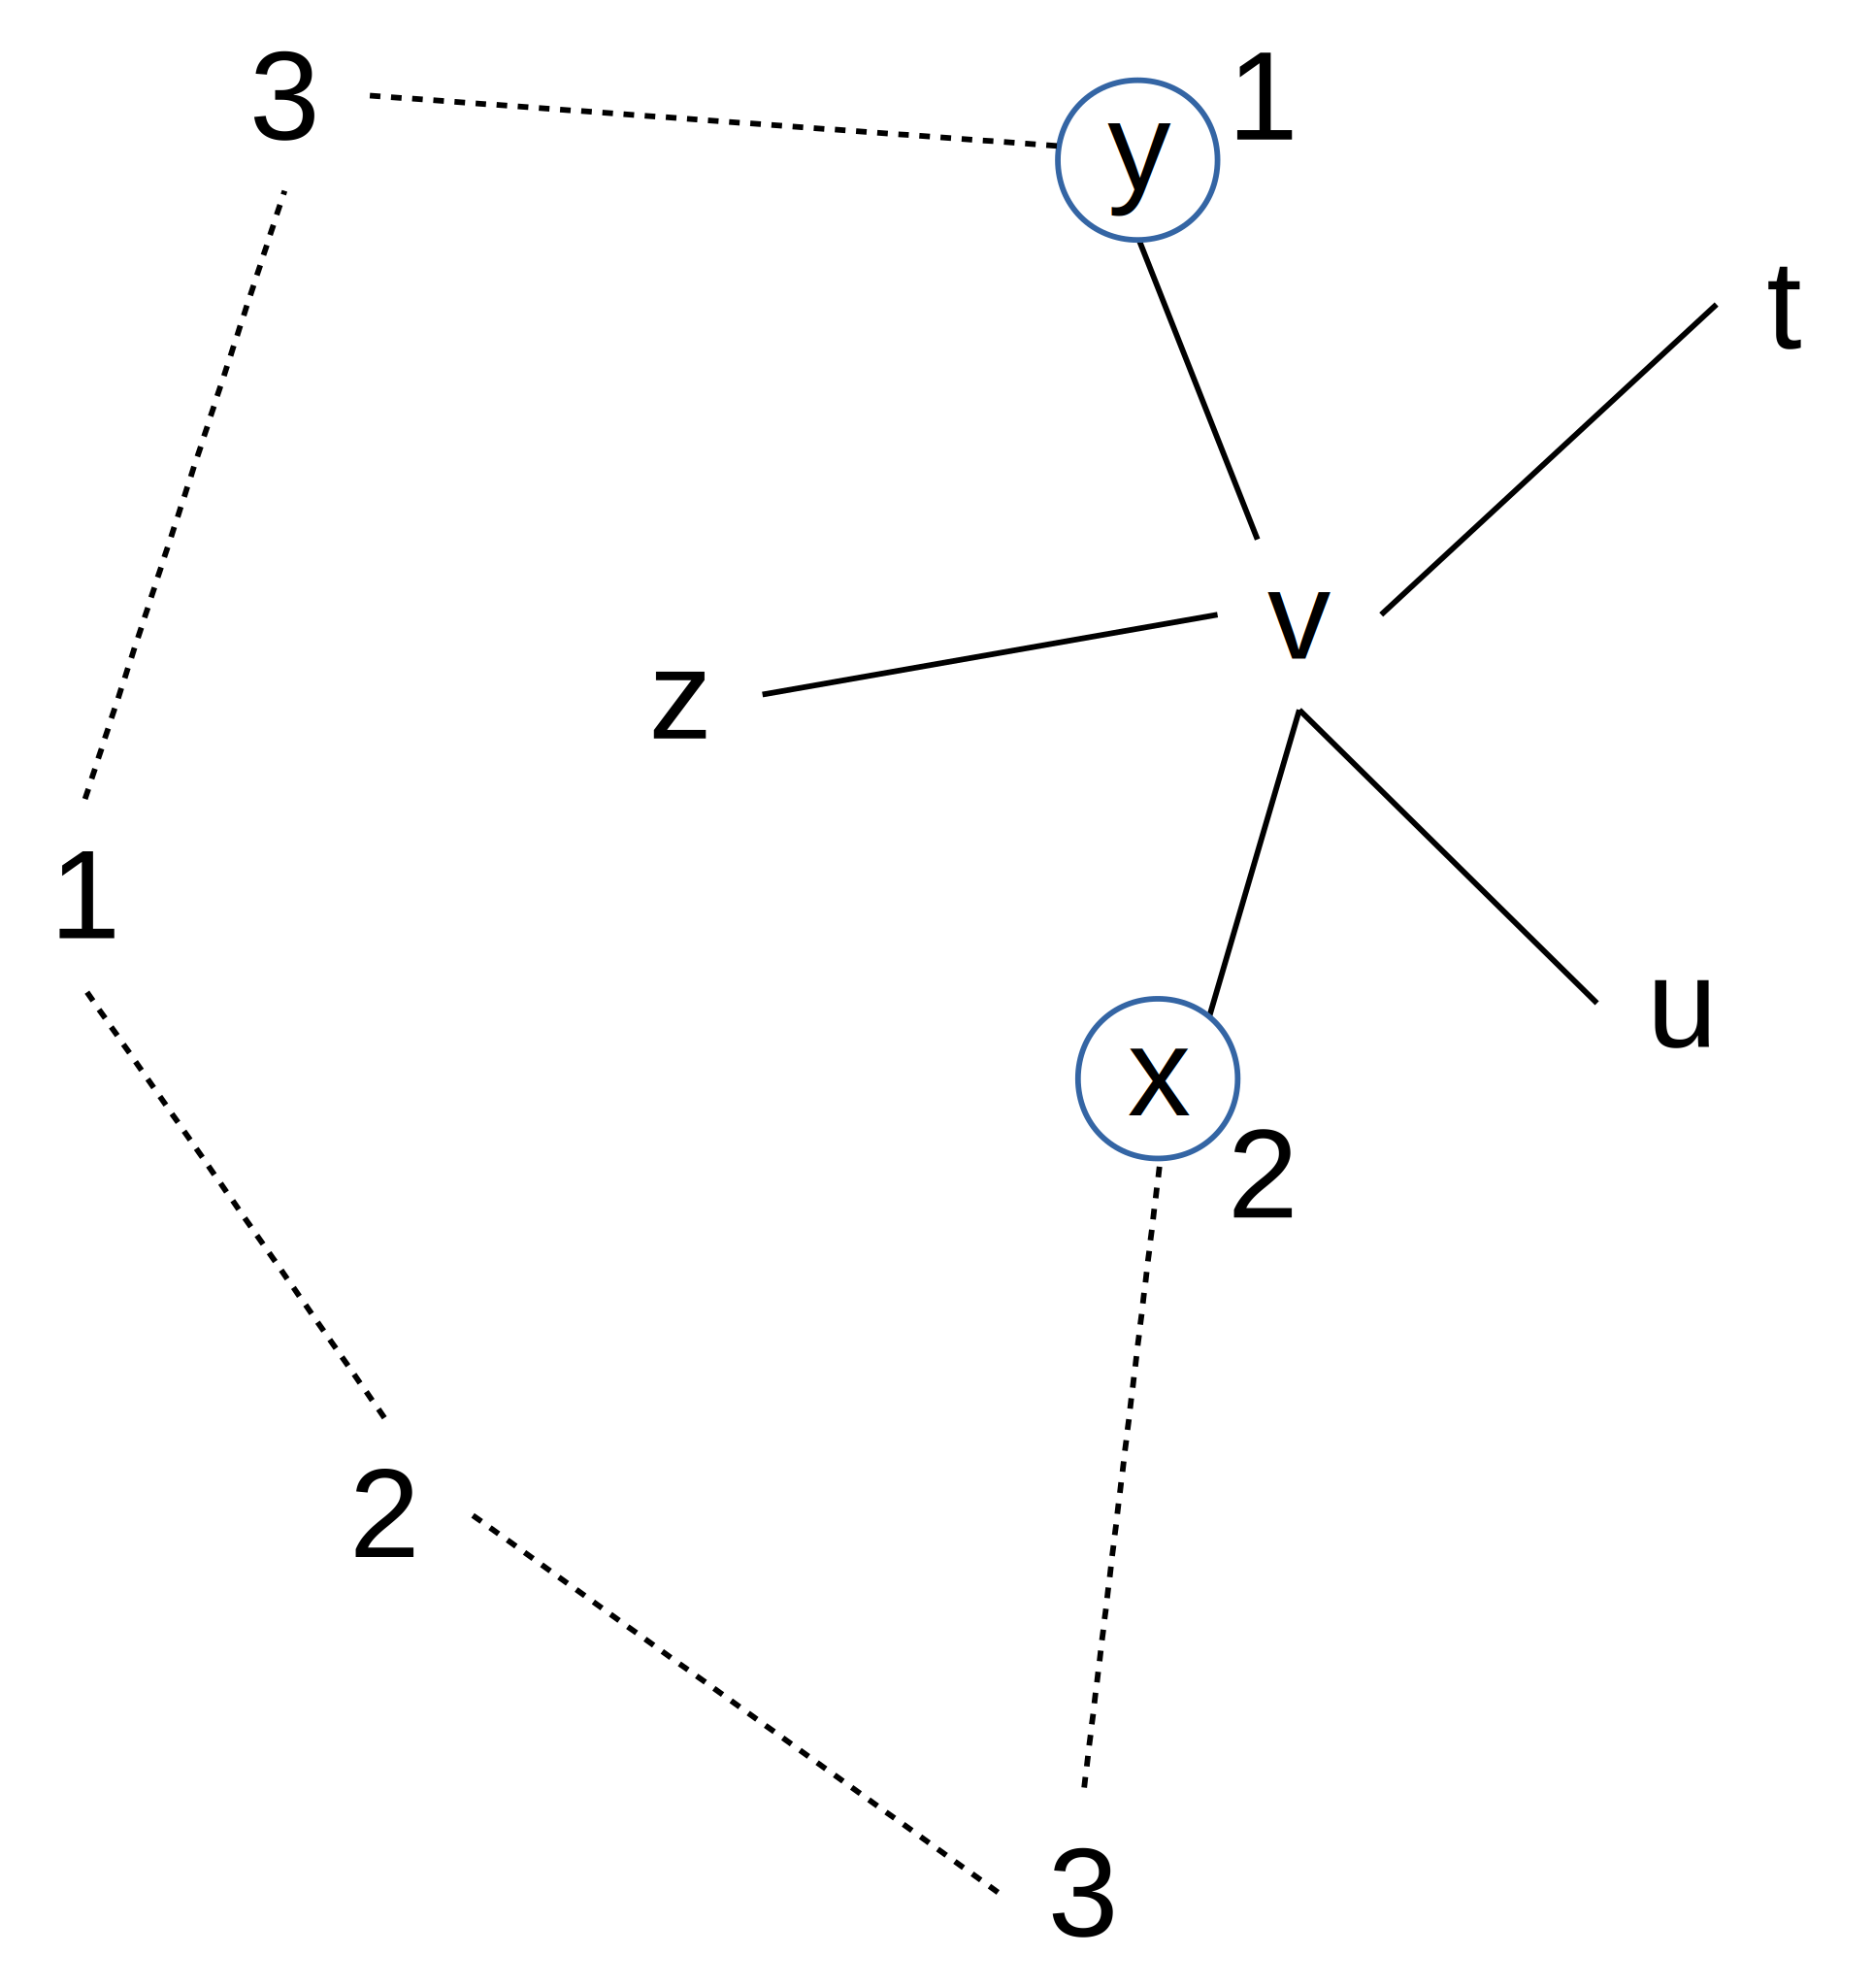
\includegraphics[scale=0.5]{lectures/161125/pix/2.pdf}
                        \begin{itemize}
                            \item betrachte 5-Färbung $\mathcal{C} \colon V(G \setminus \{v\}) \mapsto \{1, \dots, 5\}$, die es nach Rekursion gibt
                            \item betrache $x,y \in V_{xy}$ und sei $V_{xy} \subset V(G)$ die Menge der Knoten mit $\mathcal{C}(x)$- oder $\mathcal{C}(y)$-Färbung
                                \begin{enumerate}
                                    \item es gibt \underline{keinen} Weg von $x \rightsquigarrow y$, der nur Knoten aus $V_{xy}$ nutzt
                                        \begin{itemize}
                                            \item Seien $V'_{xy}$ die $s \in V(G \setminus \{v\})$, die von $x$ nur via $V_{xy}$ erreicht werden
                                            \item Färbe um:
                                            \begin{math}
                                                \mathcal{C'}(s) =
                                                    \begin{cases}
                                                        \mathcal{C}(s) & s \not \in V'_{xy}\\
                                                        \mathcal{C}(y) & s \in V'_{xy}, ~ \mathcal{C}(s) = \mathcal{C}(x)\\
                                                        \mathcal{C}(x) & s \in V'_{xy}, ~ \mathcal{C}(s) = \mathcal{C}(y)
                                                    \end{cases}
                                            \end{math}\\\\
                                            ``Tausche Farben auf $V'_{xy}$'' $\Rightarrow \mathcal{C'}(x) = \mathcal{C'}(y) = \mathcal{C}(y)$
                                        \end{itemize}
                                    \item es gibt einen solchen Pfad $x \rightsquigarrow y$ mit allen Knoten in $V_{xy}$
                                    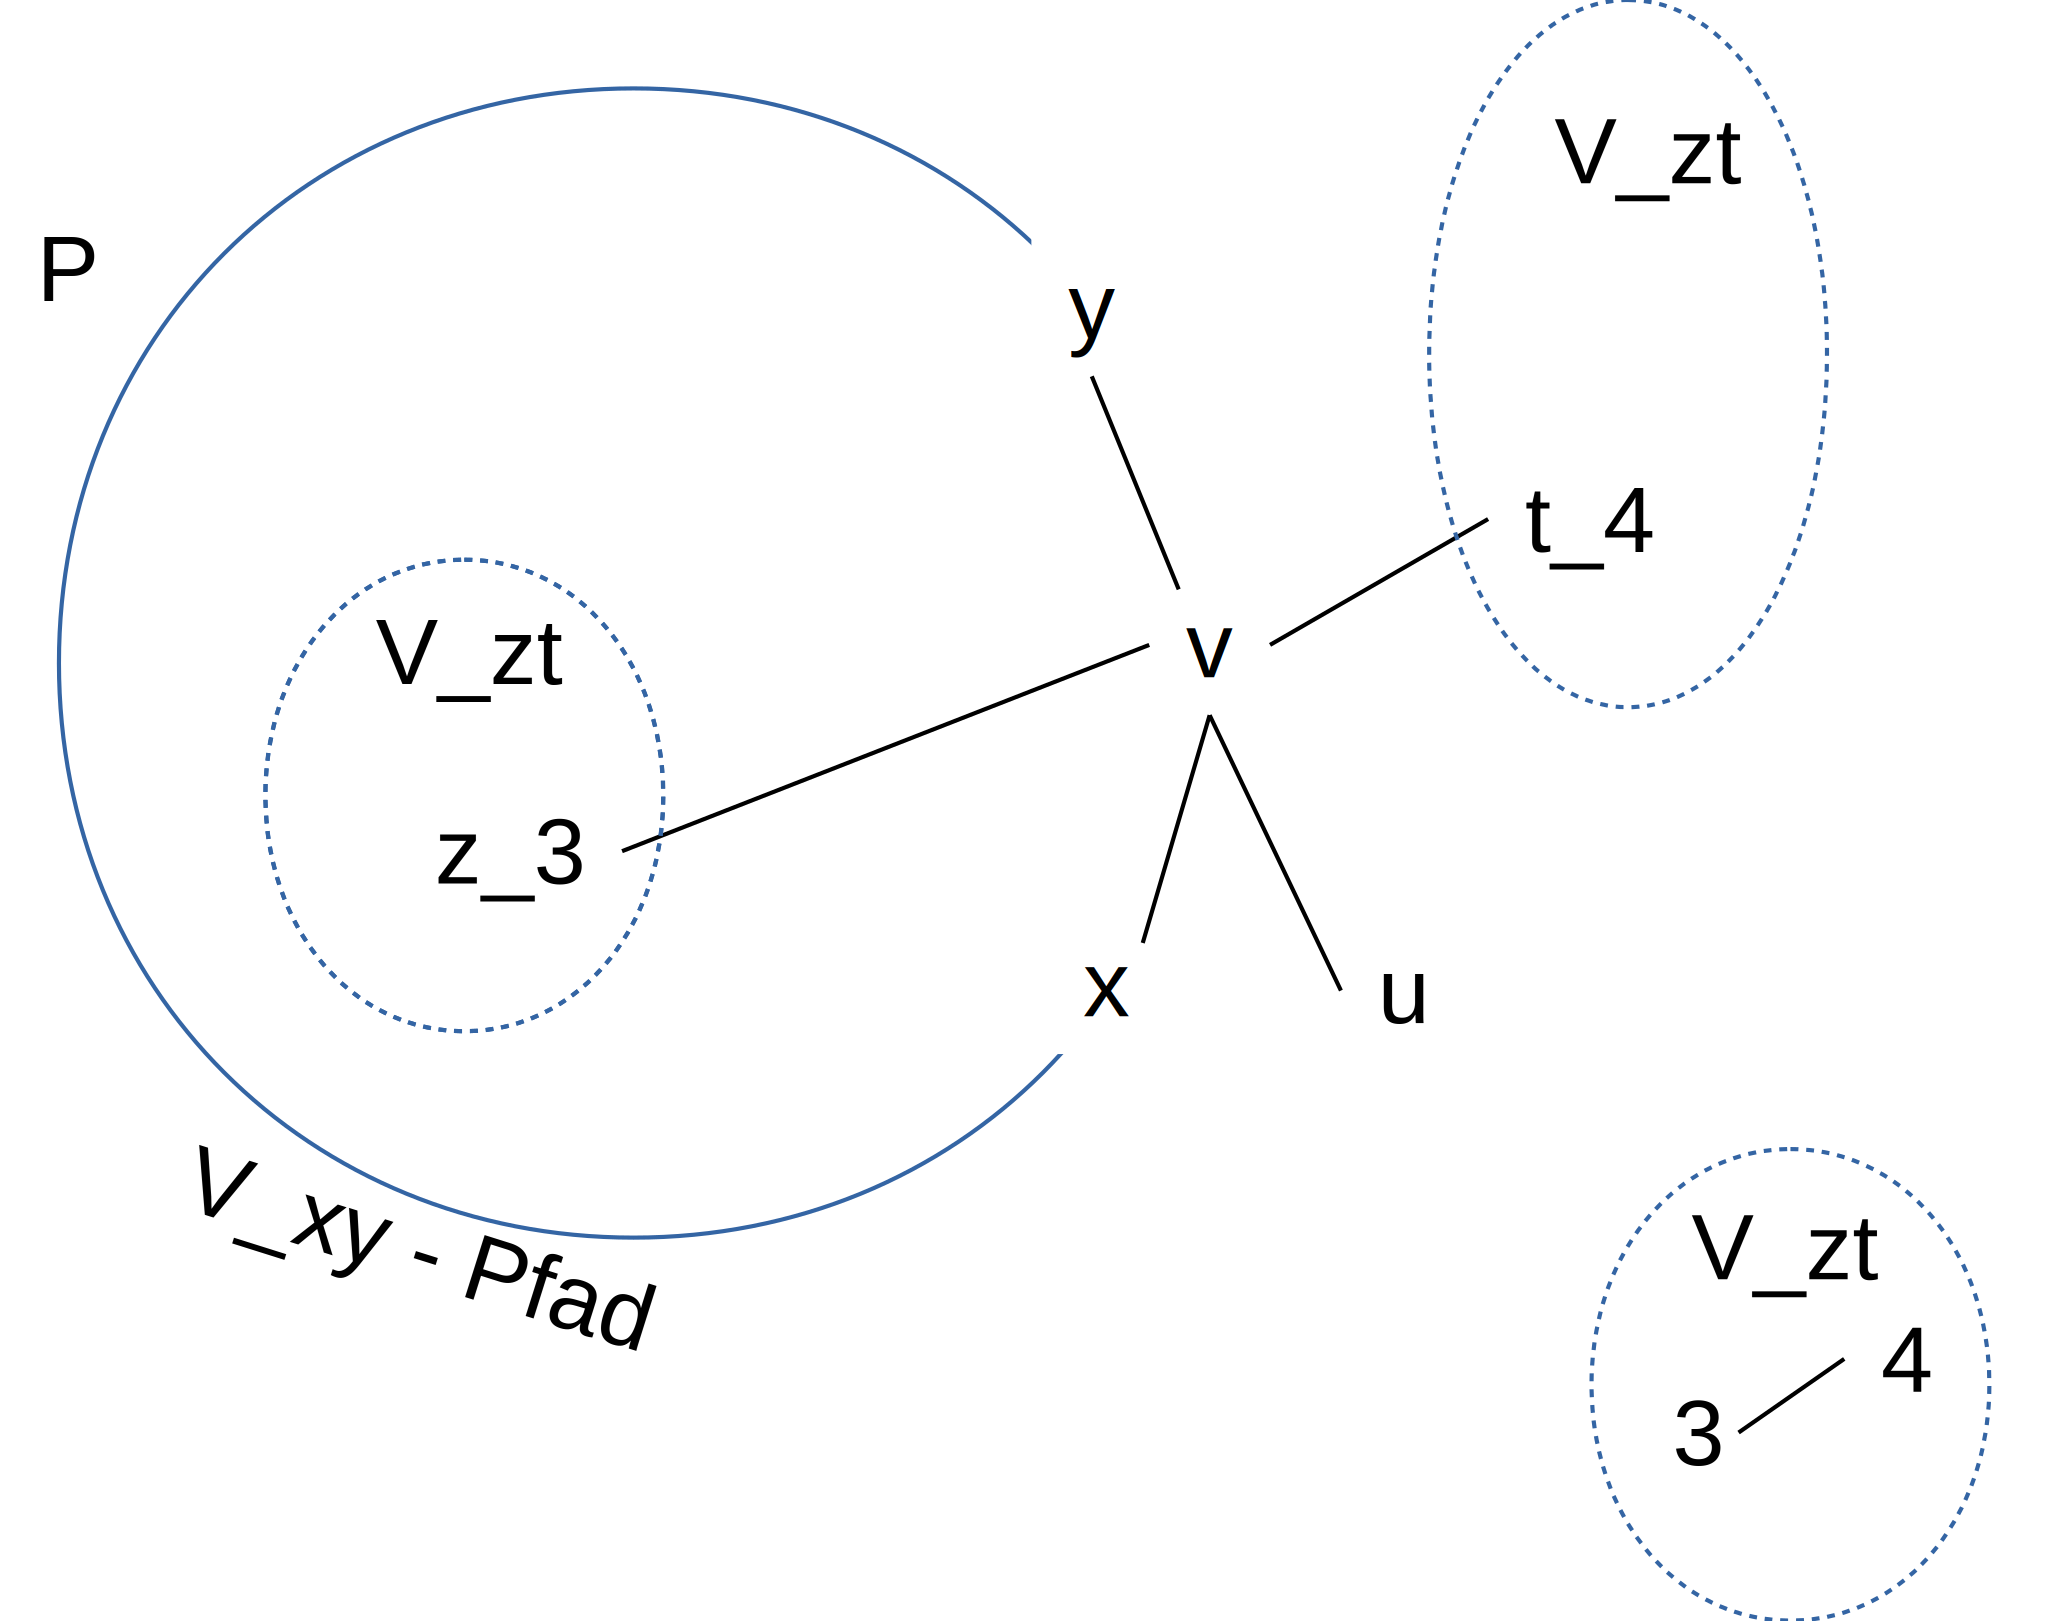
\includegraphics[scale=0.5]{lectures/161125/pix/3.pdf}
                                        \begin{itemize}
                                            \item $V_{zt}$: alle Knoten in $V(G \setminus \{v\})$, die $\mathcal{C}(t)$ oder $\mathcal{C}(z)$ gefärbt sind
                                            \item $V_{xy} \cap V_{zt} = \emptyset$!
                                            \item $V'_{zt}$ kann nur via eines $s \in P$ einen Knoten in $V_{zt} \setminus V'_{zt}$ erreichen
                                        \end{itemize}
                                        Damit lassen sich $z,t$ analog zu Fall (a) färben.
                                \end{enumerate}
                        \end{itemize}
                \end{enumerate}
        \end{description}
    \item[Theorem] Jeder planare Graph ist 4-färbbar
        \begin{description}
            \item[Proof] Es gibt eine Menge von 1936 4-färbbaren Karten, jede nicht Teil eines kleinsten Gegenbeispiels... (Appel, Haken, 1976).
            $\Rightarrow$ Es folgt, dass es kein kleinstes Gegenbeispiel gibt.
        \end{description}
\end{description}

\subsection{Zufallsgraphen}
Sei $G=(V,E)$ mit $V=\{1, \dots, n\}$ fixiert. Wir wollen nun Kanten zufällig auswählen auf dieser fixierten Kantenmenge $\{1, \dots, n\}$, um zufällige Graphen zu generieren. 
Die Menge dieser Zufallsgraphen nennen wir $\mathcal{G}$. \underline{Jede} Kante wird mit Wahrscheinlichkeit $p \in [0, \dots, 1]$ gewählt. 
Sei $G_0$ ein bestimmter Graph. Das Ereignis $\{G_0\}$ mit $G_0$ und m Kanten hat die Wahrscheinlichkeit $p^m \cdot (1-p)^{{n \over 2}-m}$. 
Wahrscheinlichkeitsmaß auf 
$\mathcal{G} ~ \forall e \in [v]^2$\\
$\Omega_e=\{0_e, 1_e\}$\\
$\mathbb{P}(\{1_e\})=p$\\
$\mathbb{P}(\{0_e\})=1-p$\\
$\Omega_\mathcal{G} = \prod\limits_{e \in [v]^2} \Omega_e$

\begin{description}
    \item[Beispiele] Fixiere Graph $H$, $V(H) = V(G)$, ist $H \leqslant G$? \\
        Mit $p^l$, $|E(H)| = l$, $|V(H)| = k$, aber falls $H$ induzierter Teilgraph von $G$ sein soll? \\
         - Nur $p^l (1-p)^{\binom{k}{2} - l}$. \\
        Und was ist mit Subgraph-Isomorphismus?
        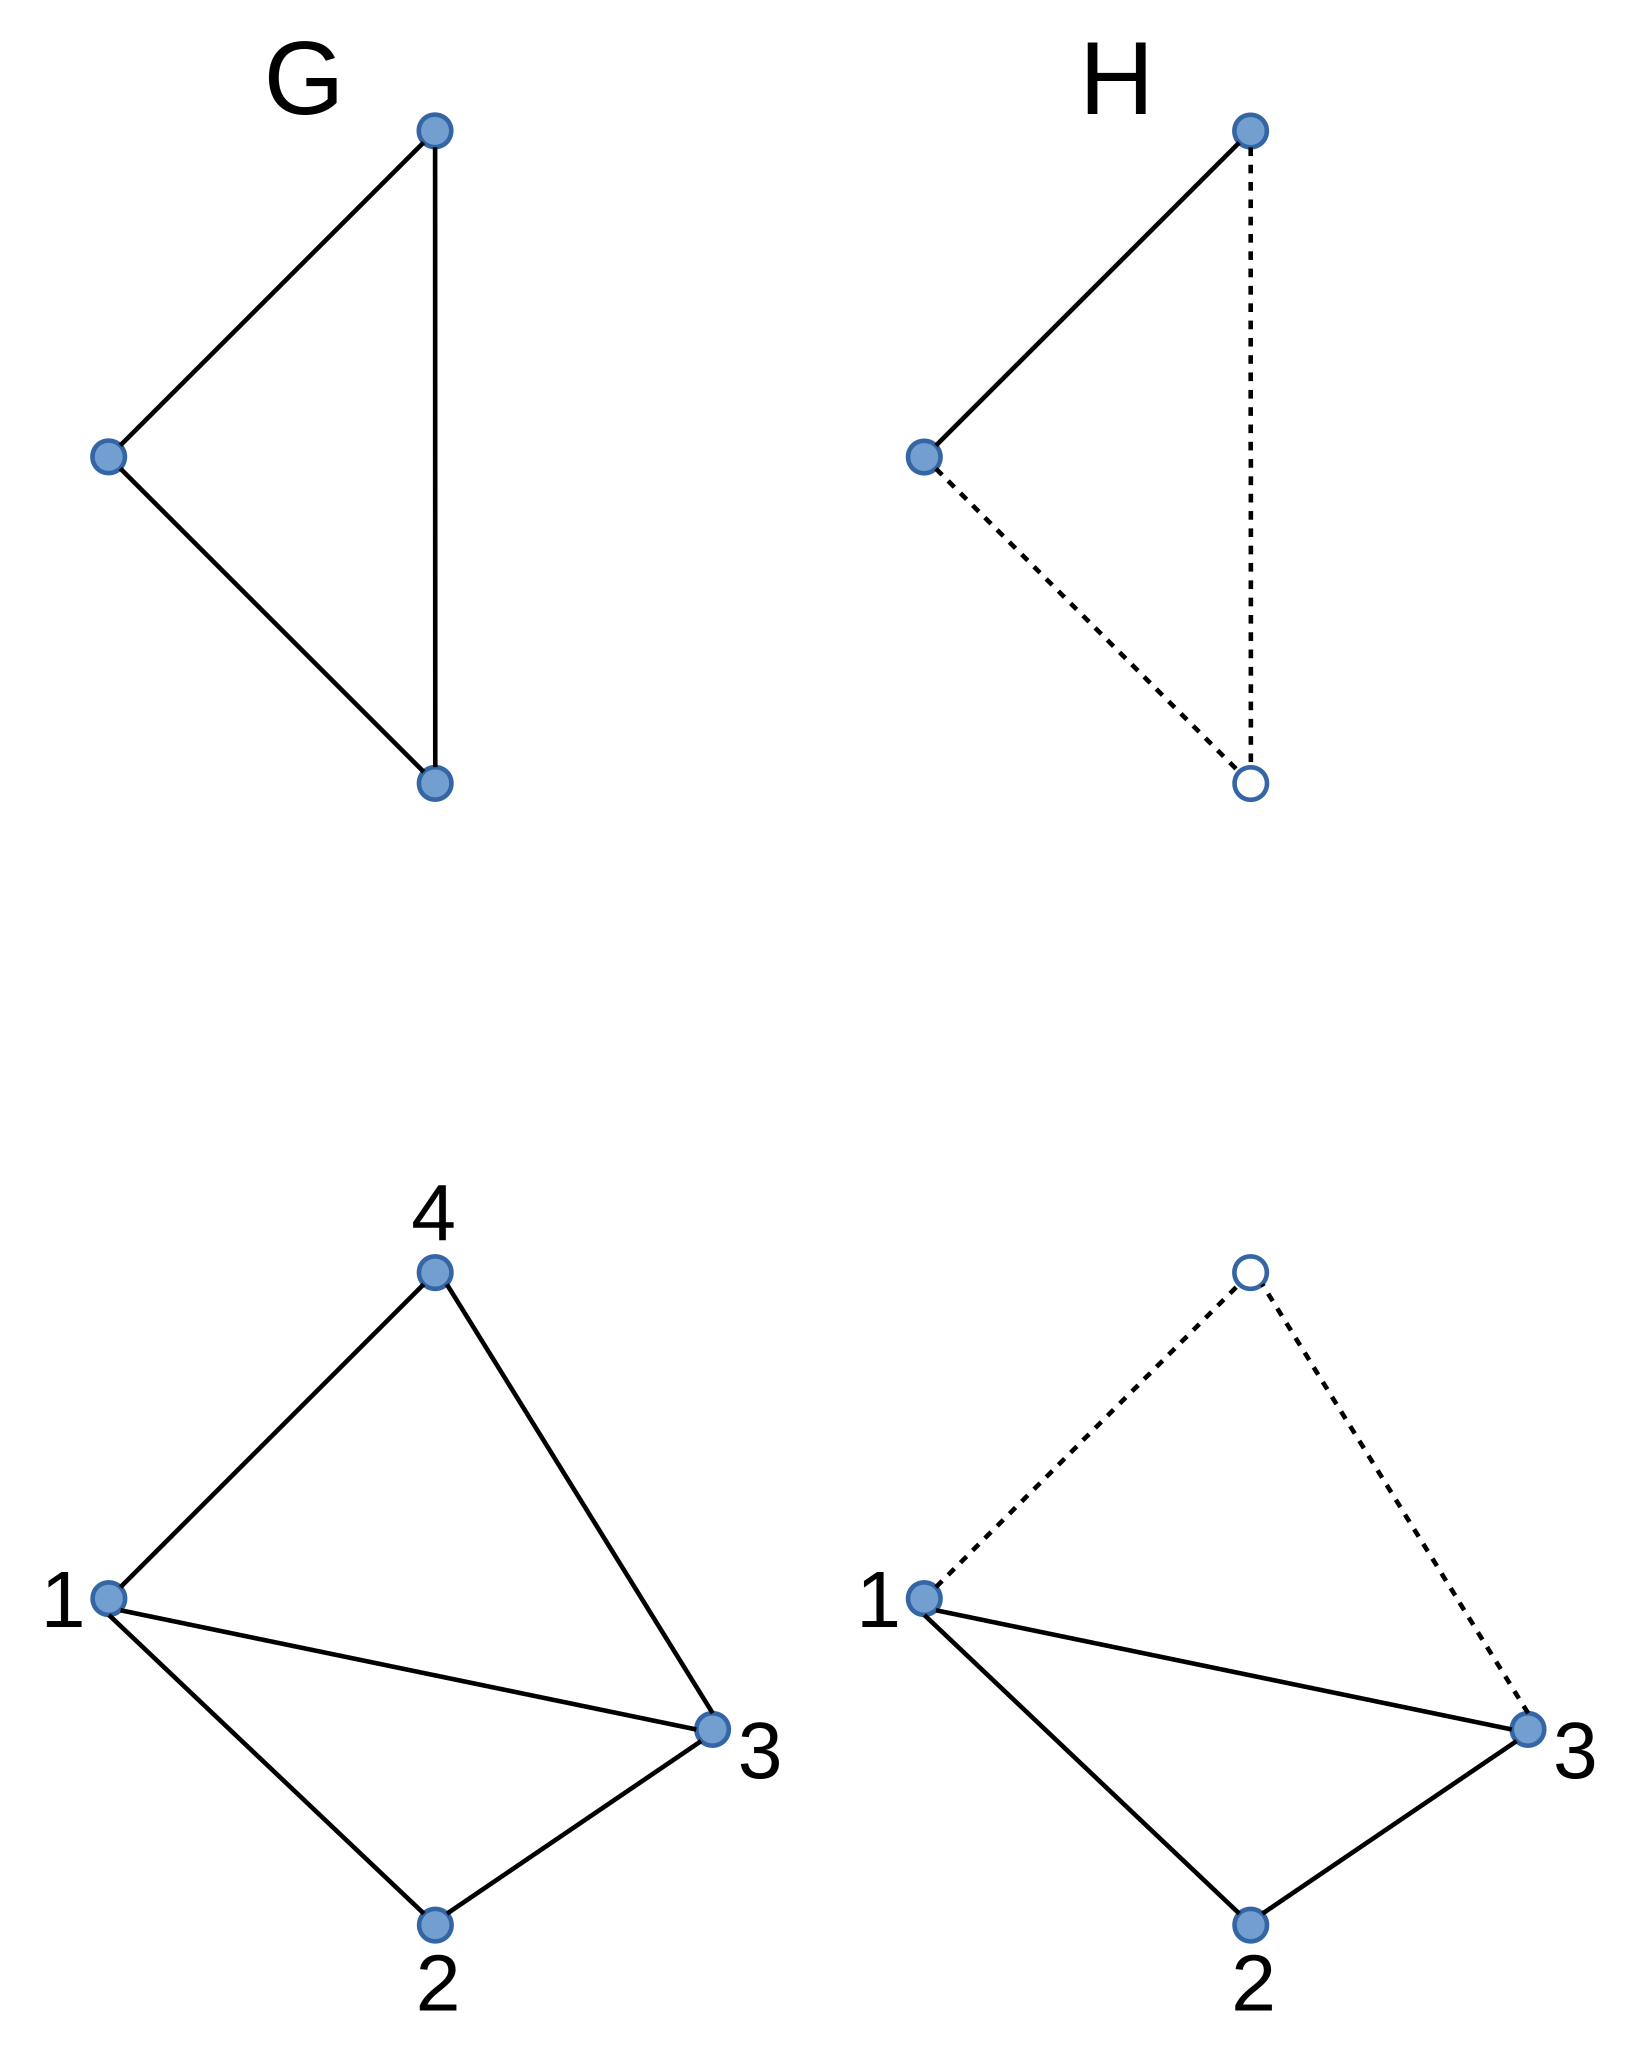
\includegraphics[scale=0.5]{lectures/161125/pix/4.pdf}
        \begin{itemize}
            \item Ereignismengen überlappen
            \item kompliziert
        \end{itemize}
\end{description}

\subsection{Eigenschaften fast aller Graphen}
Falls die Wahrscheinlichkeit, dass $P(G \in \mathcal{G}) \rightarrow 1$ für $n \rightarrow \infty$, dann geschieht $G$ fast sicher.
\begin{description}
    \item[Pro:] Gegeben jedes $H$ als Isomorphie-Klasse, $n \rightarrow \infty$ und $p \in ]0,1[ = (0,1)$, induzierte Kopie von $H$. 
    Dann haben fast alle $G$ in $\mathcal{G}(n,p)$ haben mindestens eine induzierte Kopie von $H$.
    \item[Prf:] Sei $H$ gegeben, $K=V(H)$. Sei $K \leqslant n$. $H$ ist (subgraph-) isomorph zu $G$ mit Wahrscheinlichkeit $r < 0$ ($G$ ist zufällig!). 
        Teile $G$ in $\lfloor {n \over k} \rfloor$ Teilgraphen, um genau so viele ``Versuche'' (für $r > 0$) zu haben. 
        $P(H \not \subseteq G$ induziert) $\leqslant (1-r)^{\lfloor {n \over k} \rfloor} \xrightarrow{n \rightarrow \infty} 0$
\end{description}


\newpage

\section{Vorlesung 25.11.2016}
\subsection{Färbung von Graphen}
\subsubsection{Vertexfärbung}
Zwei durch eine Kante verbundene Knoten haben unterschiedliche Farben.\\
Beispiel wäre eine Landkarte auf der mit so wenig wie möglich Farben die Länder ausgemalt werden, ohne zwei benachbarte Länder gleichfarbig zu haben. Hierbei entspricht jede Facette einen Knoten.\\
\includegraphics[width=0.4\textwidth]{lectures/161125/pix/Vertexfaerbung}
\begin{description}
    \item[Vertexfärbung] Eine Vertexfärbung eines Graphen $G=(V,E)$ ist eine Abbildung $\mathcal{C} \colon V \mapsto \mathcal{S}$, mit $\mathcal{S}=$ Menge der Farben. Es gilt, dass $\mathcal{C}(v) \neq \mathcal{C}(w)$, mit $w,v \in \mathcal{S}$, wenn $v$ und $w$ adjazent ($\{v,w\} \in E$) sind. Die Elemente von $\mathcal{S}$ heißen \emph{Farben}.
    \item[k-Färbung] Ein Graph $G$ ist $k$-färbbar, wenn es für eine Abbildung $\mathcal{C}$ eine Menge $\mathcal{S}=\{1,\dots,k\}$ gibt.
    \item[Chromatische Zahl] Eine chromatische Zahl $\chi(G)$ ist die kleinste natürliche Zahl $k$, sodass G $k$-färbbar ist. $\chi(G) \leqslant \Delta(G) + 1$, mit $\Delta(G) = $ maximaler Grad von $G$
        \begin{description}
            \item[Proof (greedy)] Färbe $v_i$ der Vertices $v_1 \dots v_n$ mit der kleinsten Farbe, die nicht von einem Nachbarn von $v_i$ benutzt wird. Da wir max. $\Delta(G)$ viele Nachbarn für $v_i$ haben, gibt es immer eine freie Farbe.
        \end{description}
        $\chi(G) \geqslant$ Größe der größten Clique
    \item[Lemma] Für jeden einfachen planaren Graphen $G$ ist der Durchschnittsgrad $d(G) < 6$
        \begin{description}
            \item[Proof] $d(G) = 2 \cdot {|E| \over |V|}$ mit $|V| \leqslant 3$, $|E| \leqslant 3  \cdot |V| - 6$, dann $d(G) \leqslant {2(3 \cdot |V|-6) \over |V|} = 6-{12 \over |V|}$
        \end{description}
    \item[Theorem] Jeder simple planare Graph $G$ hat $\chi(G) \leqslant 6$
        \begin{description}
            \item[Proof] Annahme: Jeder simple planare Graph mit $|V| = n$ ist $6$-färbbar.
            \begin{itemize}
                \item Sei $G$ hiermit ein simpler planarer Graph mit $|V| = n+1$
                \item Vom Lemma wissen wir, dass $w \in V$ mit $d(w) \leqslant 5$ existiert
                \item Sei $G' = G \setminus \{w\}$. Via Induktionshypothese ist $G'$ 6-färbbar. Das tun wir dann.
                \item Färbe $w$ mit der (min.) freien Farbe, um $G$ zu färben
            \end{itemize}
        \end{description}
    \item[Theorem] Für jeden simplen planaren Graphen $G$ gilt, dass $\chi(G) \leqslant 5$
        \begin{description}
            \item[Proof] Sei $G=(V,E)$ planar
                \begin{enumerate}
                    \item Falls $|V| \leqslant 5 \rightarrow$ trivial
                    \item Für alle $v \in V(G)$ mit $deg(v) < 5$, färbe $v$ und arbeite mit $G \setminus \{v\}$
                    \item $G$ hat Vertex $v$ mit $deg(v) = 5$
                        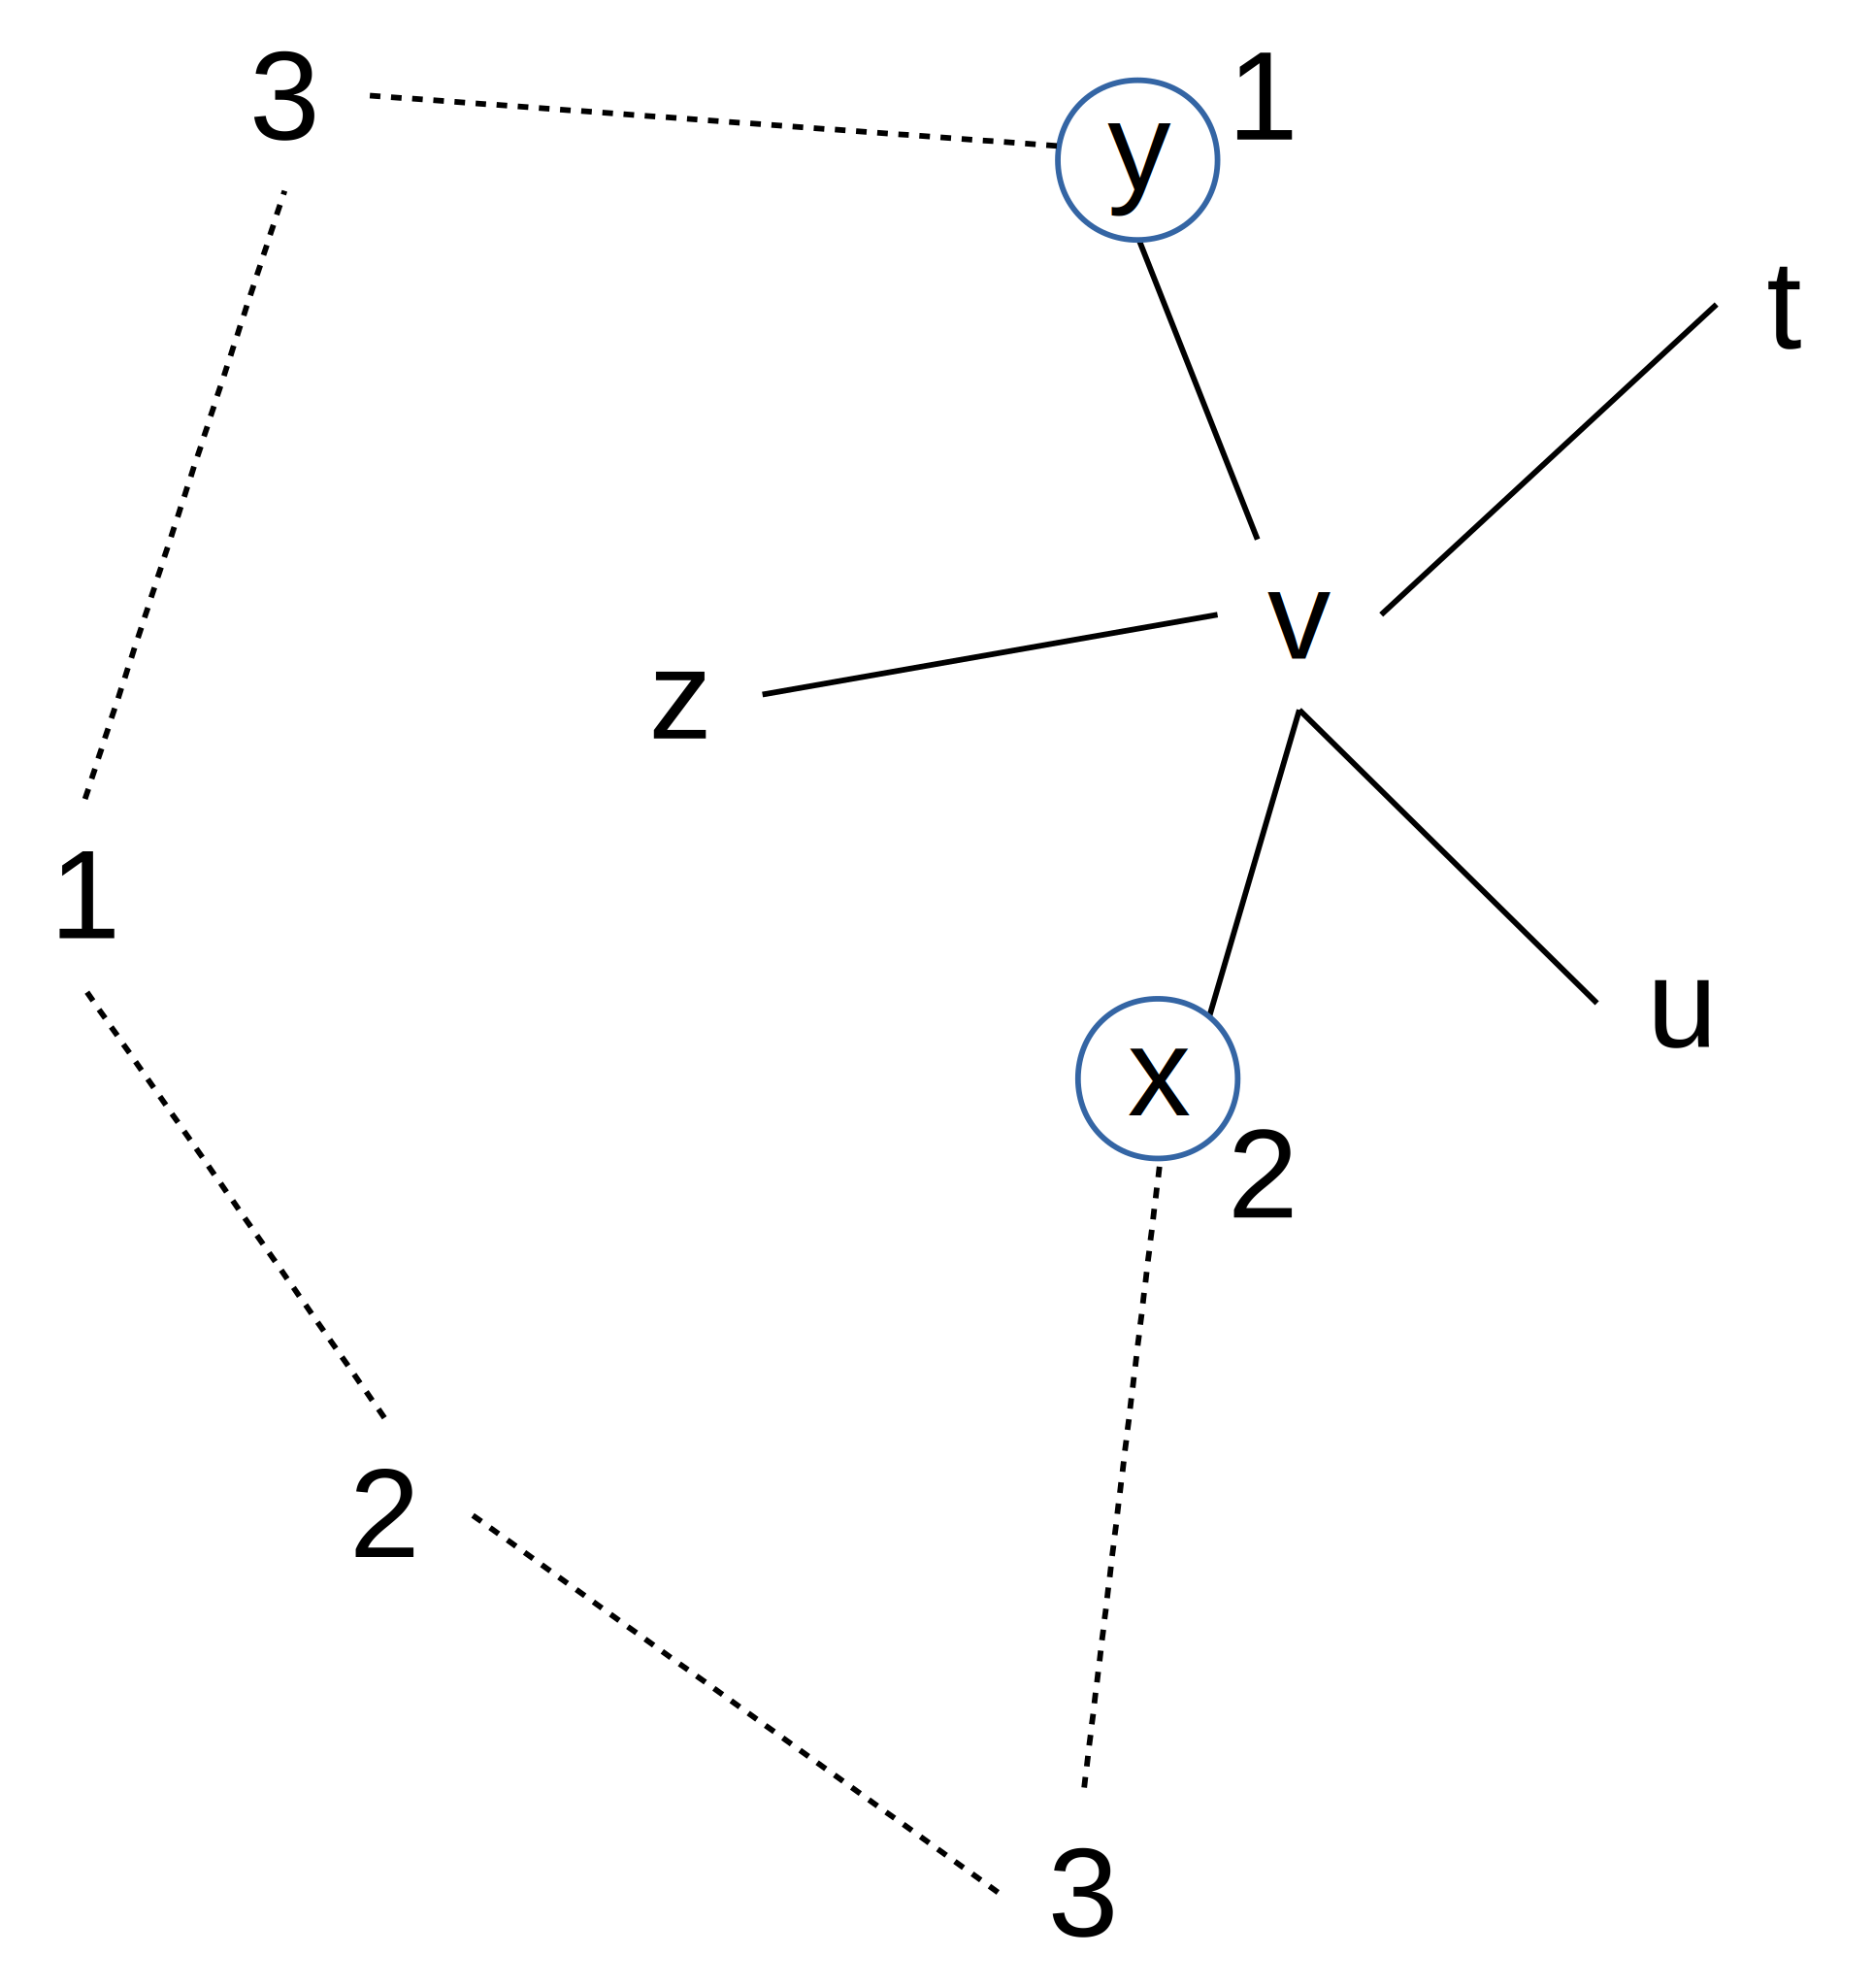
\includegraphics[scale=0.5]{lectures/161125/pix/2.pdf}
                        \begin{itemize}
                            \item betrachte 5-Färbung $\mathcal{C} \colon V(G \setminus \{v\}) \mapsto \{1, \dots, 5\}$, die es nach Rekursion gibt
                            \item betrache $x,y \in V_{xy}$ und sei $V_{xy} \subset V(G)$ die Menge der Knoten mit $\mathcal{C}(x)$- oder $\mathcal{C}(y)$-Färbung
                                \begin{enumerate}
                                    \item es gibt \underline{keinen} Weg von $x \rightsquigarrow y$, der nur Knoten aus $V_{xy}$ nutzt
                                        \begin{itemize}
                                            \item Seien $V'_{xy}$ die $s \in V(G \setminus \{v\})$, die von $x$ nur via $V_{xy}$ erreicht werden
                                            \item Färbe um:
                                            \begin{math}
                                                \mathcal{C'}(s) =
                                                    \begin{cases}
                                                        \mathcal{C}(s) & s \not \in V'_{xy}\\
                                                        \mathcal{C}(y) & s \in V'_{xy}, ~ \mathcal{C}(s) = \mathcal{C}(x)\\
                                                        \mathcal{C}(x) & s \in V'_{xy}, ~ \mathcal{C}(s) = \mathcal{C}(y)
                                                    \end{cases}
                                            \end{math}\\\\
                                            ``Tausche Farben auf $V'_{xy}$'' $\Rightarrow \mathcal{C'}(x) = \mathcal{C'}(y) = \mathcal{C}(y)$
                                        \end{itemize}
                                    \item es gibt einen solchen Pfad $x \rightsquigarrow y$ mit allen Knoten in $V_{xy}$
                                    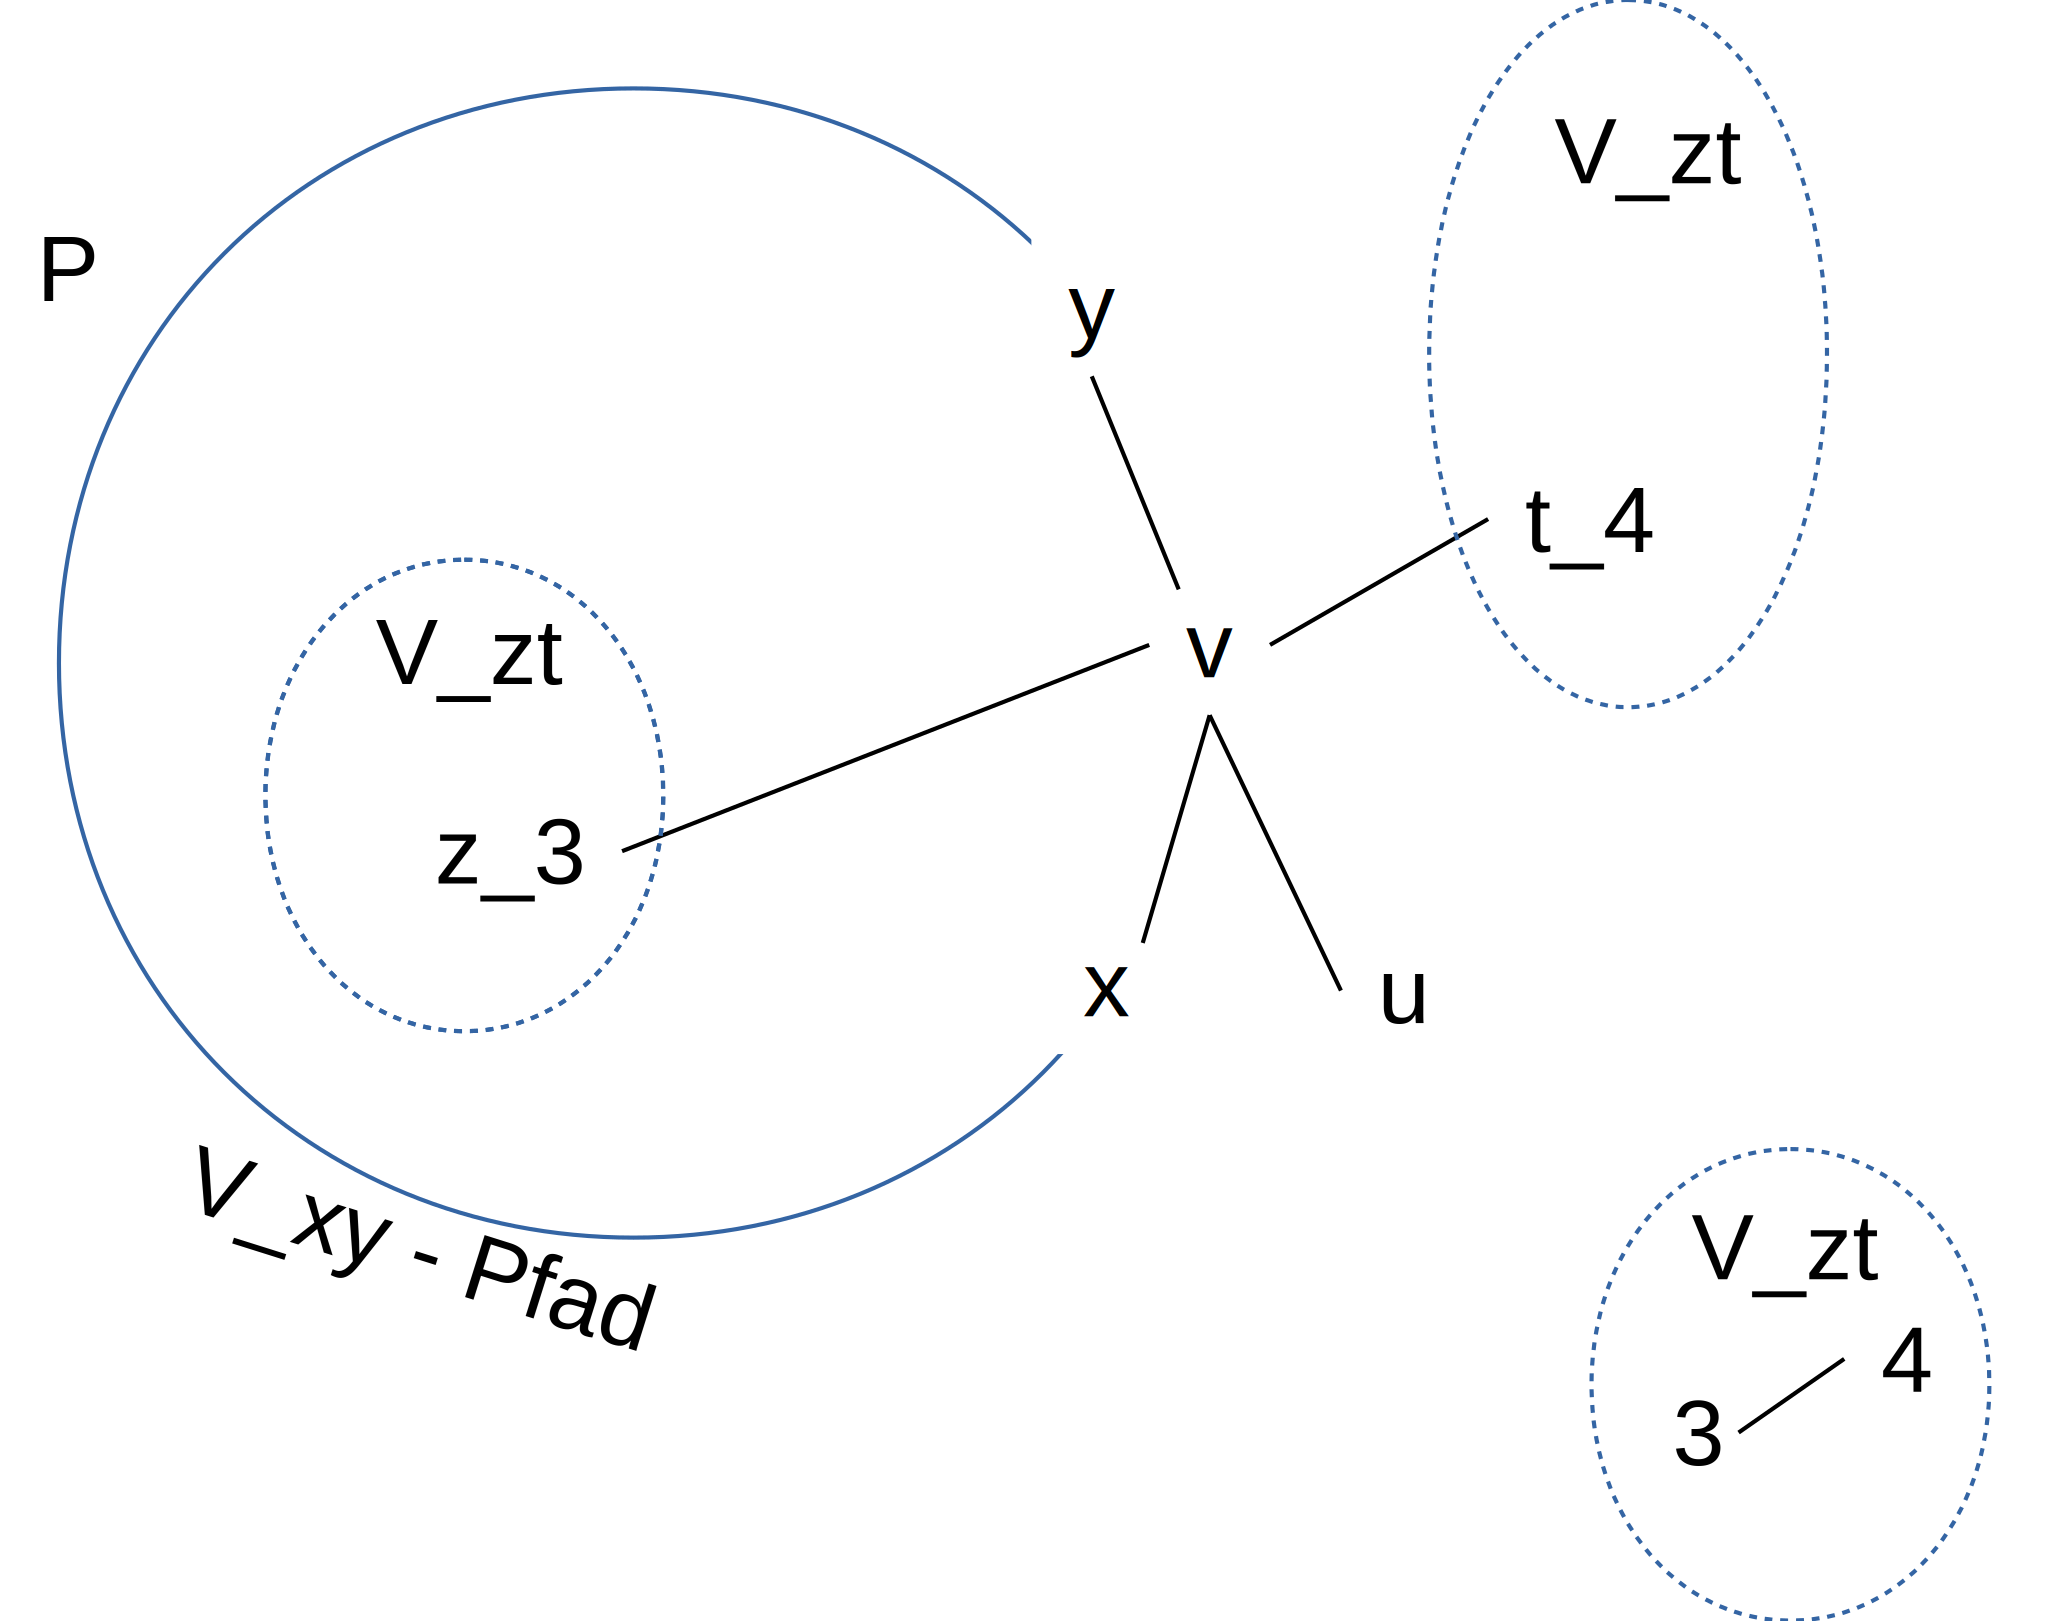
\includegraphics[scale=0.5]{lectures/161125/pix/3.pdf}
                                        \begin{itemize}
                                            \item $V_{zt}$: alle Knoten in $V(G \setminus \{v\})$, die $\mathcal{C}(t)$ oder $\mathcal{C}(z)$ gefärbt sind
                                            \item $V_{xy} \cap V_{zt} = \emptyset$!
                                            \item $V'_{zt}$ kann nur via eines $s \in P$ einen Knoten in $V_{zt} \setminus V'_{zt}$ erreichen
                                        \end{itemize}
                                        Damit lassen sich $z,t$ analog zu Fall (a) färben.
                                \end{enumerate}
                        \end{itemize}
                \end{enumerate}
        \end{description}
    \item[Theorem] Jeder planare Graph ist 4-färbbar
        \begin{description}
            \item[Proof] Es gibt eine Menge von 1936 4-färbbaren Karten, jede nicht Teil eines kleinsten Gegenbeispiels... (Appel, Haken, 1976).
            $\Rightarrow$ Es folgt, dass es kein kleinstes Gegenbeispiel gibt.
        \end{description}
\end{description}

\subsection{Zufallsgraphen}
Sei $G=(V,E)$ mit $V=\{1, \dots, n\}$ fixiert. Wir wollen nun Kanten zufällig auswählen auf dieser fixierten Kantenmenge $\{1, \dots, n\}$, um zufällige Graphen zu generieren. 
Die Menge dieser Zufallsgraphen nennen wir $\mathcal{G}$. \underline{Jede} Kante wird mit Wahrscheinlichkeit $p \in [0, \dots, 1]$ gewählt. 
Sei $G_0$ ein bestimmter Graph. Das Ereignis $\{G_0\}$ mit $G_0$ und m Kanten hat die Wahrscheinlichkeit $p^m \cdot (1-p)^{{n \over 2}-m}$. 
Wahrscheinlichkeitsmaß auf 
$\mathcal{G} ~ \forall e \in [v]^2$\\
$\Omega_e=\{0_e, 1_e\}$\\
$\mathbb{P}(\{1_e\})=p$\\
$\mathbb{P}(\{0_e\})=1-p$\\
$\Omega_\mathcal{G} = \prod\limits_{e \in [v]^2} \Omega_e$

\begin{description}
    \item[Beispiele] Fixiere Graph $H$, $V(H) = V(G)$, ist $H \leqslant G$? \\
        Mit $p^l$, $|E(H)| = l$, $|V(H)| = k$, aber falls $H$ induzierter Teilgraph von $G$ sein soll? \\
         - Nur $p^l (1-p)^{\binom{k}{2} - l}$. \\
        Und was ist mit Subgraph-Isomorphismus?
        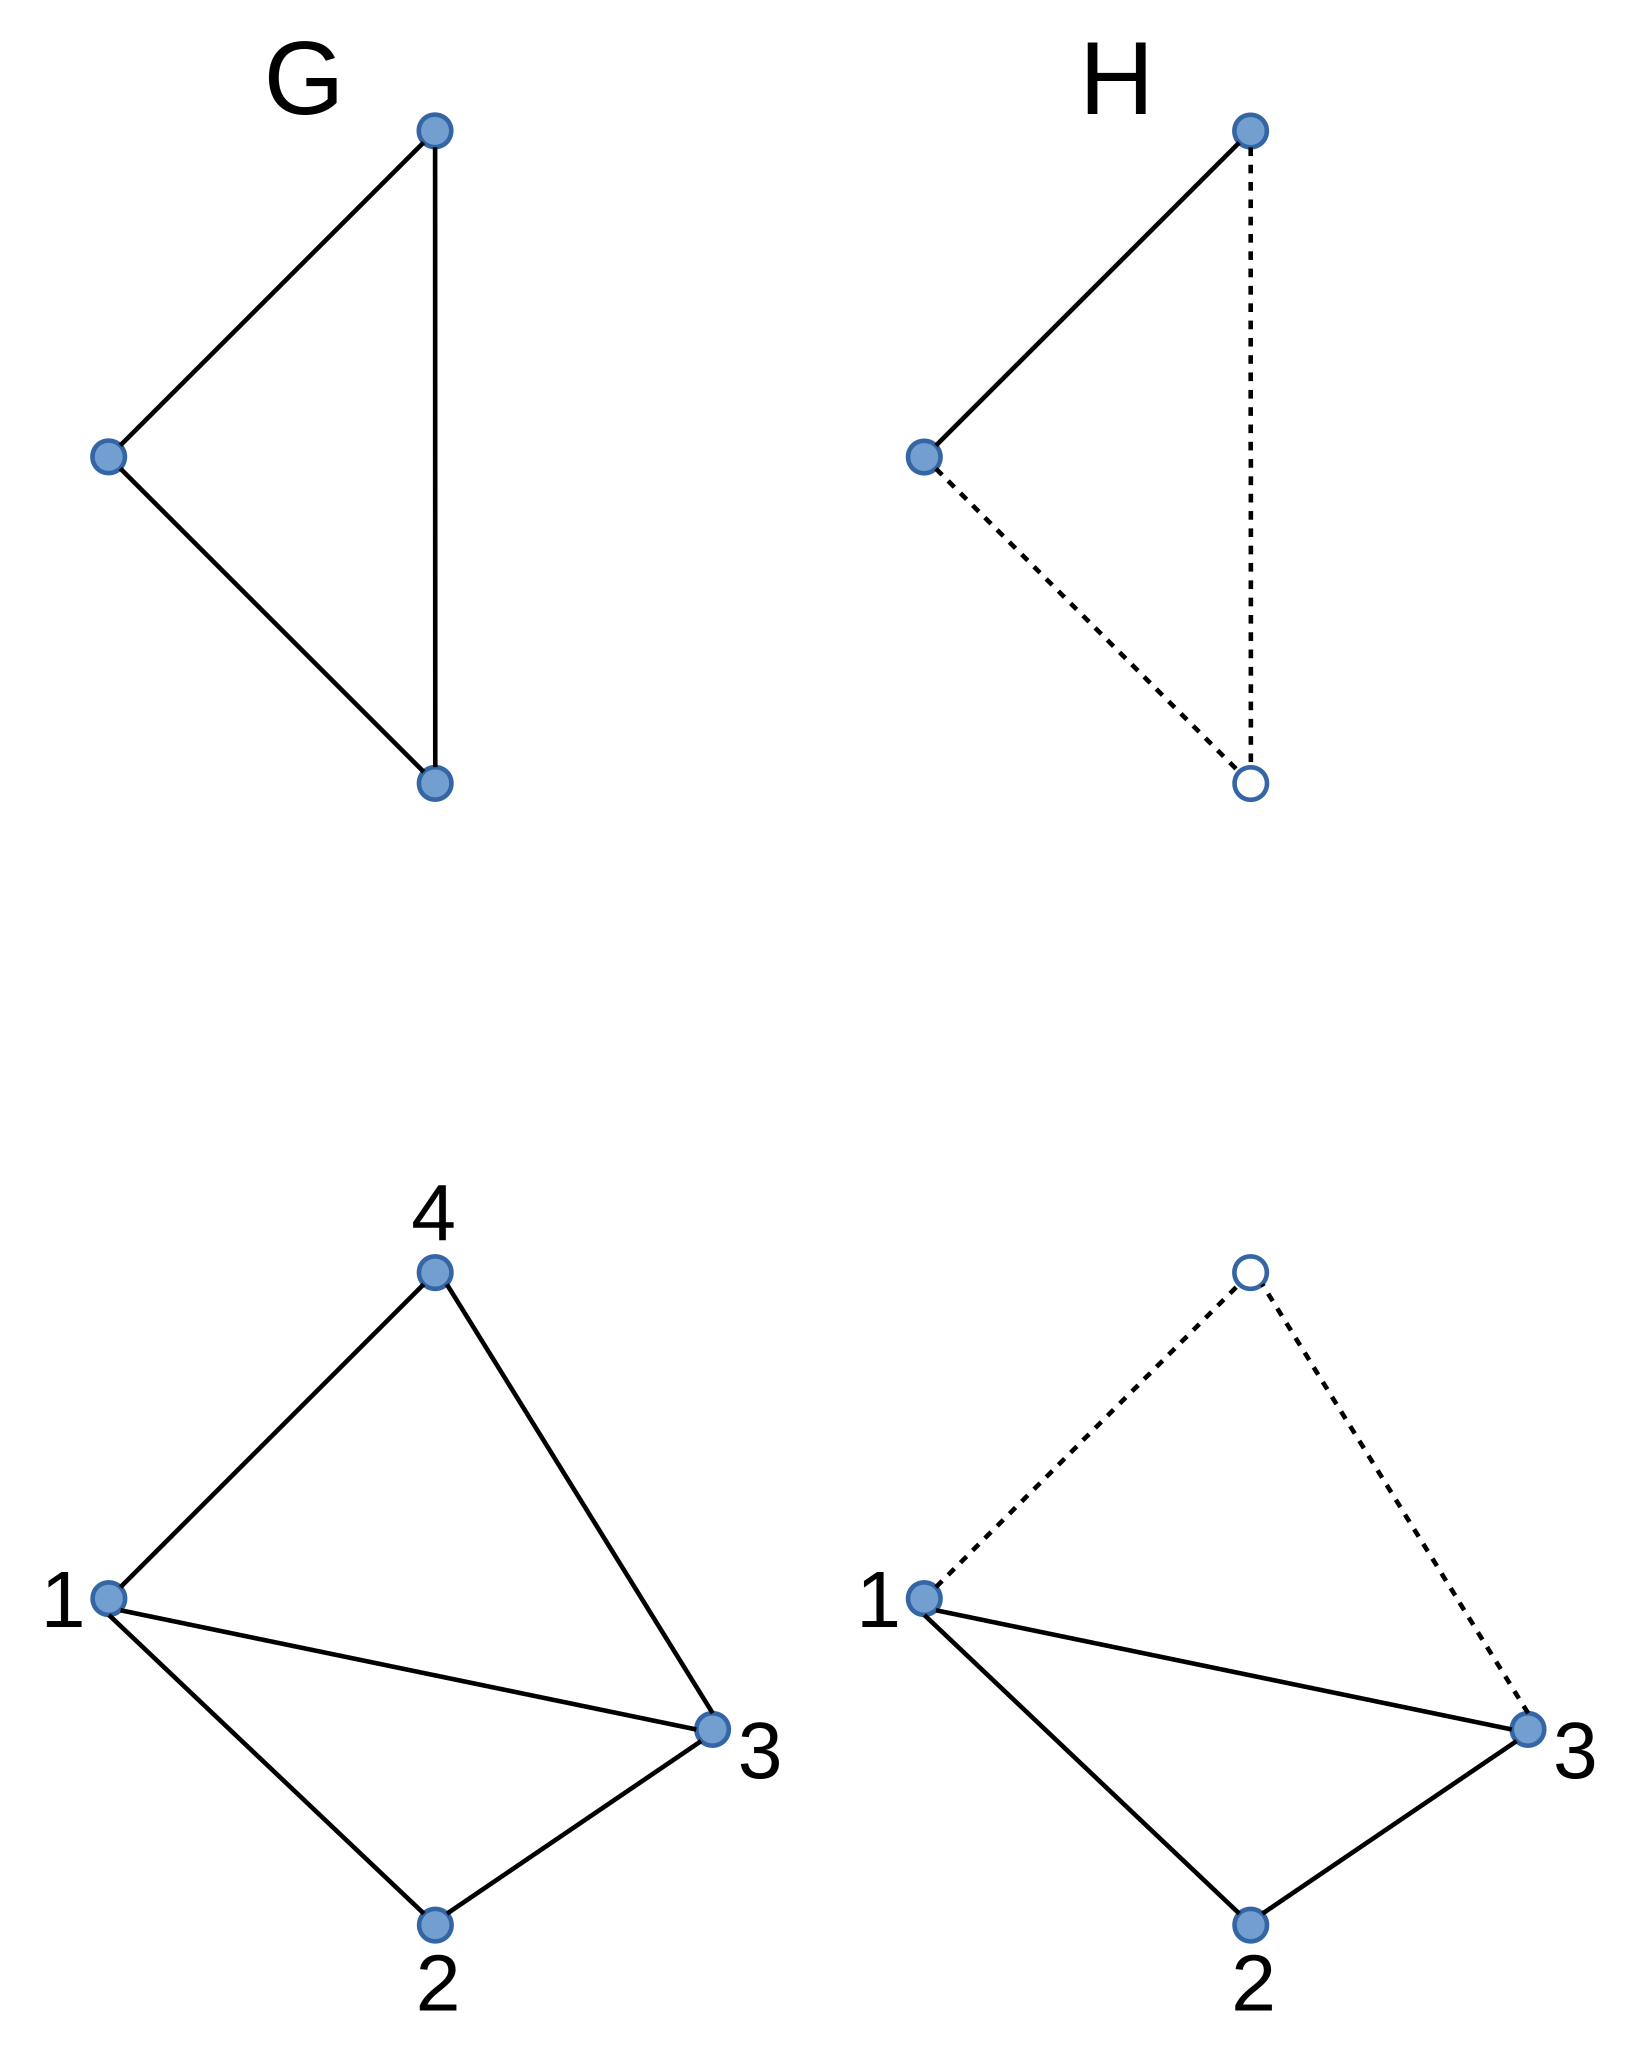
\includegraphics[scale=0.5]{lectures/161125/pix/4.pdf}
        \begin{itemize}
            \item Ereignismengen überlappen
            \item kompliziert
        \end{itemize}
\end{description}

\subsection{Eigenschaften fast aller Graphen}
Falls die Wahrscheinlichkeit, dass $P(G \in \mathcal{G}) \rightarrow 1$ für $n \rightarrow \infty$, dann geschieht $G$ fast sicher.
\begin{description}
    \item[Pro:] Gegeben jedes $H$ als Isomorphie-Klasse, $n \rightarrow \infty$ und $p \in ]0,1[ = (0,1)$, induzierte Kopie von $H$. 
    Dann haben fast alle $G$ in $\mathcal{G}(n,p)$ haben mindestens eine induzierte Kopie von $H$.
    \item[Prf:] Sei $H$ gegeben, $K=V(H)$. Sei $K \leqslant n$. $H$ ist (subgraph-) isomorph zu $G$ mit Wahrscheinlichkeit $r < 0$ ($G$ ist zufällig!). 
        Teile $G$ in $\lfloor {n \over k} \rfloor$ Teilgraphen, um genau so viele ``Versuche'' (für $r > 0$) zu haben. 
        $P(H \not \subseteq G$ induziert) $\leqslant (1-r)^{\lfloor {n \over k} \rfloor} \xrightarrow{n \rightarrow \infty} 0$
\end{description}


\newpage

\section{Vorlesung 25.11.2016}
\subsection{Färbung von Graphen}
\subsubsection{Vertexfärbung}
Zwei durch eine Kante verbundene Knoten haben unterschiedliche Farben.\\
Beispiel wäre eine Landkarte auf der mit so wenig wie möglich Farben die Länder ausgemalt werden, ohne zwei benachbarte Länder gleichfarbig zu haben. Hierbei entspricht jede Facette einen Knoten.\\
\includegraphics[width=0.4\textwidth]{lectures/161125/pix/Vertexfaerbung}
\begin{description}
    \item[Vertexfärbung] Eine Vertexfärbung eines Graphen $G=(V,E)$ ist eine Abbildung $\mathcal{C} \colon V \mapsto \mathcal{S}$, mit $\mathcal{S}=$ Menge der Farben. Es gilt, dass $\mathcal{C}(v) \neq \mathcal{C}(w)$, mit $w,v \in \mathcal{S}$, wenn $v$ und $w$ adjazent ($\{v,w\} \in E$) sind. Die Elemente von $\mathcal{S}$ heißen \emph{Farben}.
    \item[k-Färbung] Ein Graph $G$ ist $k$-färbbar, wenn es für eine Abbildung $\mathcal{C}$ eine Menge $\mathcal{S}=\{1,\dots,k\}$ gibt.
    \item[Chromatische Zahl] Eine chromatische Zahl $\chi(G)$ ist die kleinste natürliche Zahl $k$, sodass G $k$-färbbar ist. $\chi(G) \leqslant \Delta(G) + 1$, mit $\Delta(G) = $ maximaler Grad von $G$
        \begin{description}
            \item[Proof (greedy)] Färbe $v_i$ der Vertices $v_1 \dots v_n$ mit der kleinsten Farbe, die nicht von einem Nachbarn von $v_i$ benutzt wird. Da wir max. $\Delta(G)$ viele Nachbarn für $v_i$ haben, gibt es immer eine freie Farbe.
        \end{description}
        $\chi(G) \geqslant$ Größe der größten Clique
    \item[Lemma] Für jeden einfachen planaren Graphen $G$ ist der Durchschnittsgrad $d(G) < 6$
        \begin{description}
            \item[Proof] $d(G) = 2 \cdot {|E| \over |V|}$ mit $|V| \leqslant 3$, $|E| \leqslant 3  \cdot |V| - 6$, dann $d(G) \leqslant {2(3 \cdot |V|-6) \over |V|} = 6-{12 \over |V|}$
        \end{description}
    \item[Theorem] Jeder simple planare Graph $G$ hat $\chi(G) \leqslant 6$
        \begin{description}
            \item[Proof] Annahme: Jeder simple planare Graph mit $|V| = n$ ist $6$-färbbar.
            \begin{itemize}
                \item Sei $G$ hiermit ein simpler planarer Graph mit $|V| = n+1$
                \item Vom Lemma wissen wir, dass $w \in V$ mit $d(w) \leqslant 5$ existiert
                \item Sei $G' = G \setminus \{w\}$. Via Induktionshypothese ist $G'$ 6-färbbar. Das tun wir dann.
                \item Färbe $w$ mit der (min.) freien Farbe, um $G$ zu färben
            \end{itemize}
        \end{description}
    \item[Theorem] Für jeden simplen planaren Graphen $G$ gilt, dass $\chi(G) \leqslant 5$
        \begin{description}
            \item[Proof] Sei $G=(V,E)$ planar
                \begin{enumerate}
                    \item Falls $|V| \leqslant 5 \rightarrow$ trivial
                    \item Für alle $v \in V(G)$ mit $deg(v) < 5$, färbe $v$ und arbeite mit $G \setminus \{v\}$
                    \item $G$ hat Vertex $v$ mit $deg(v) = 5$
                        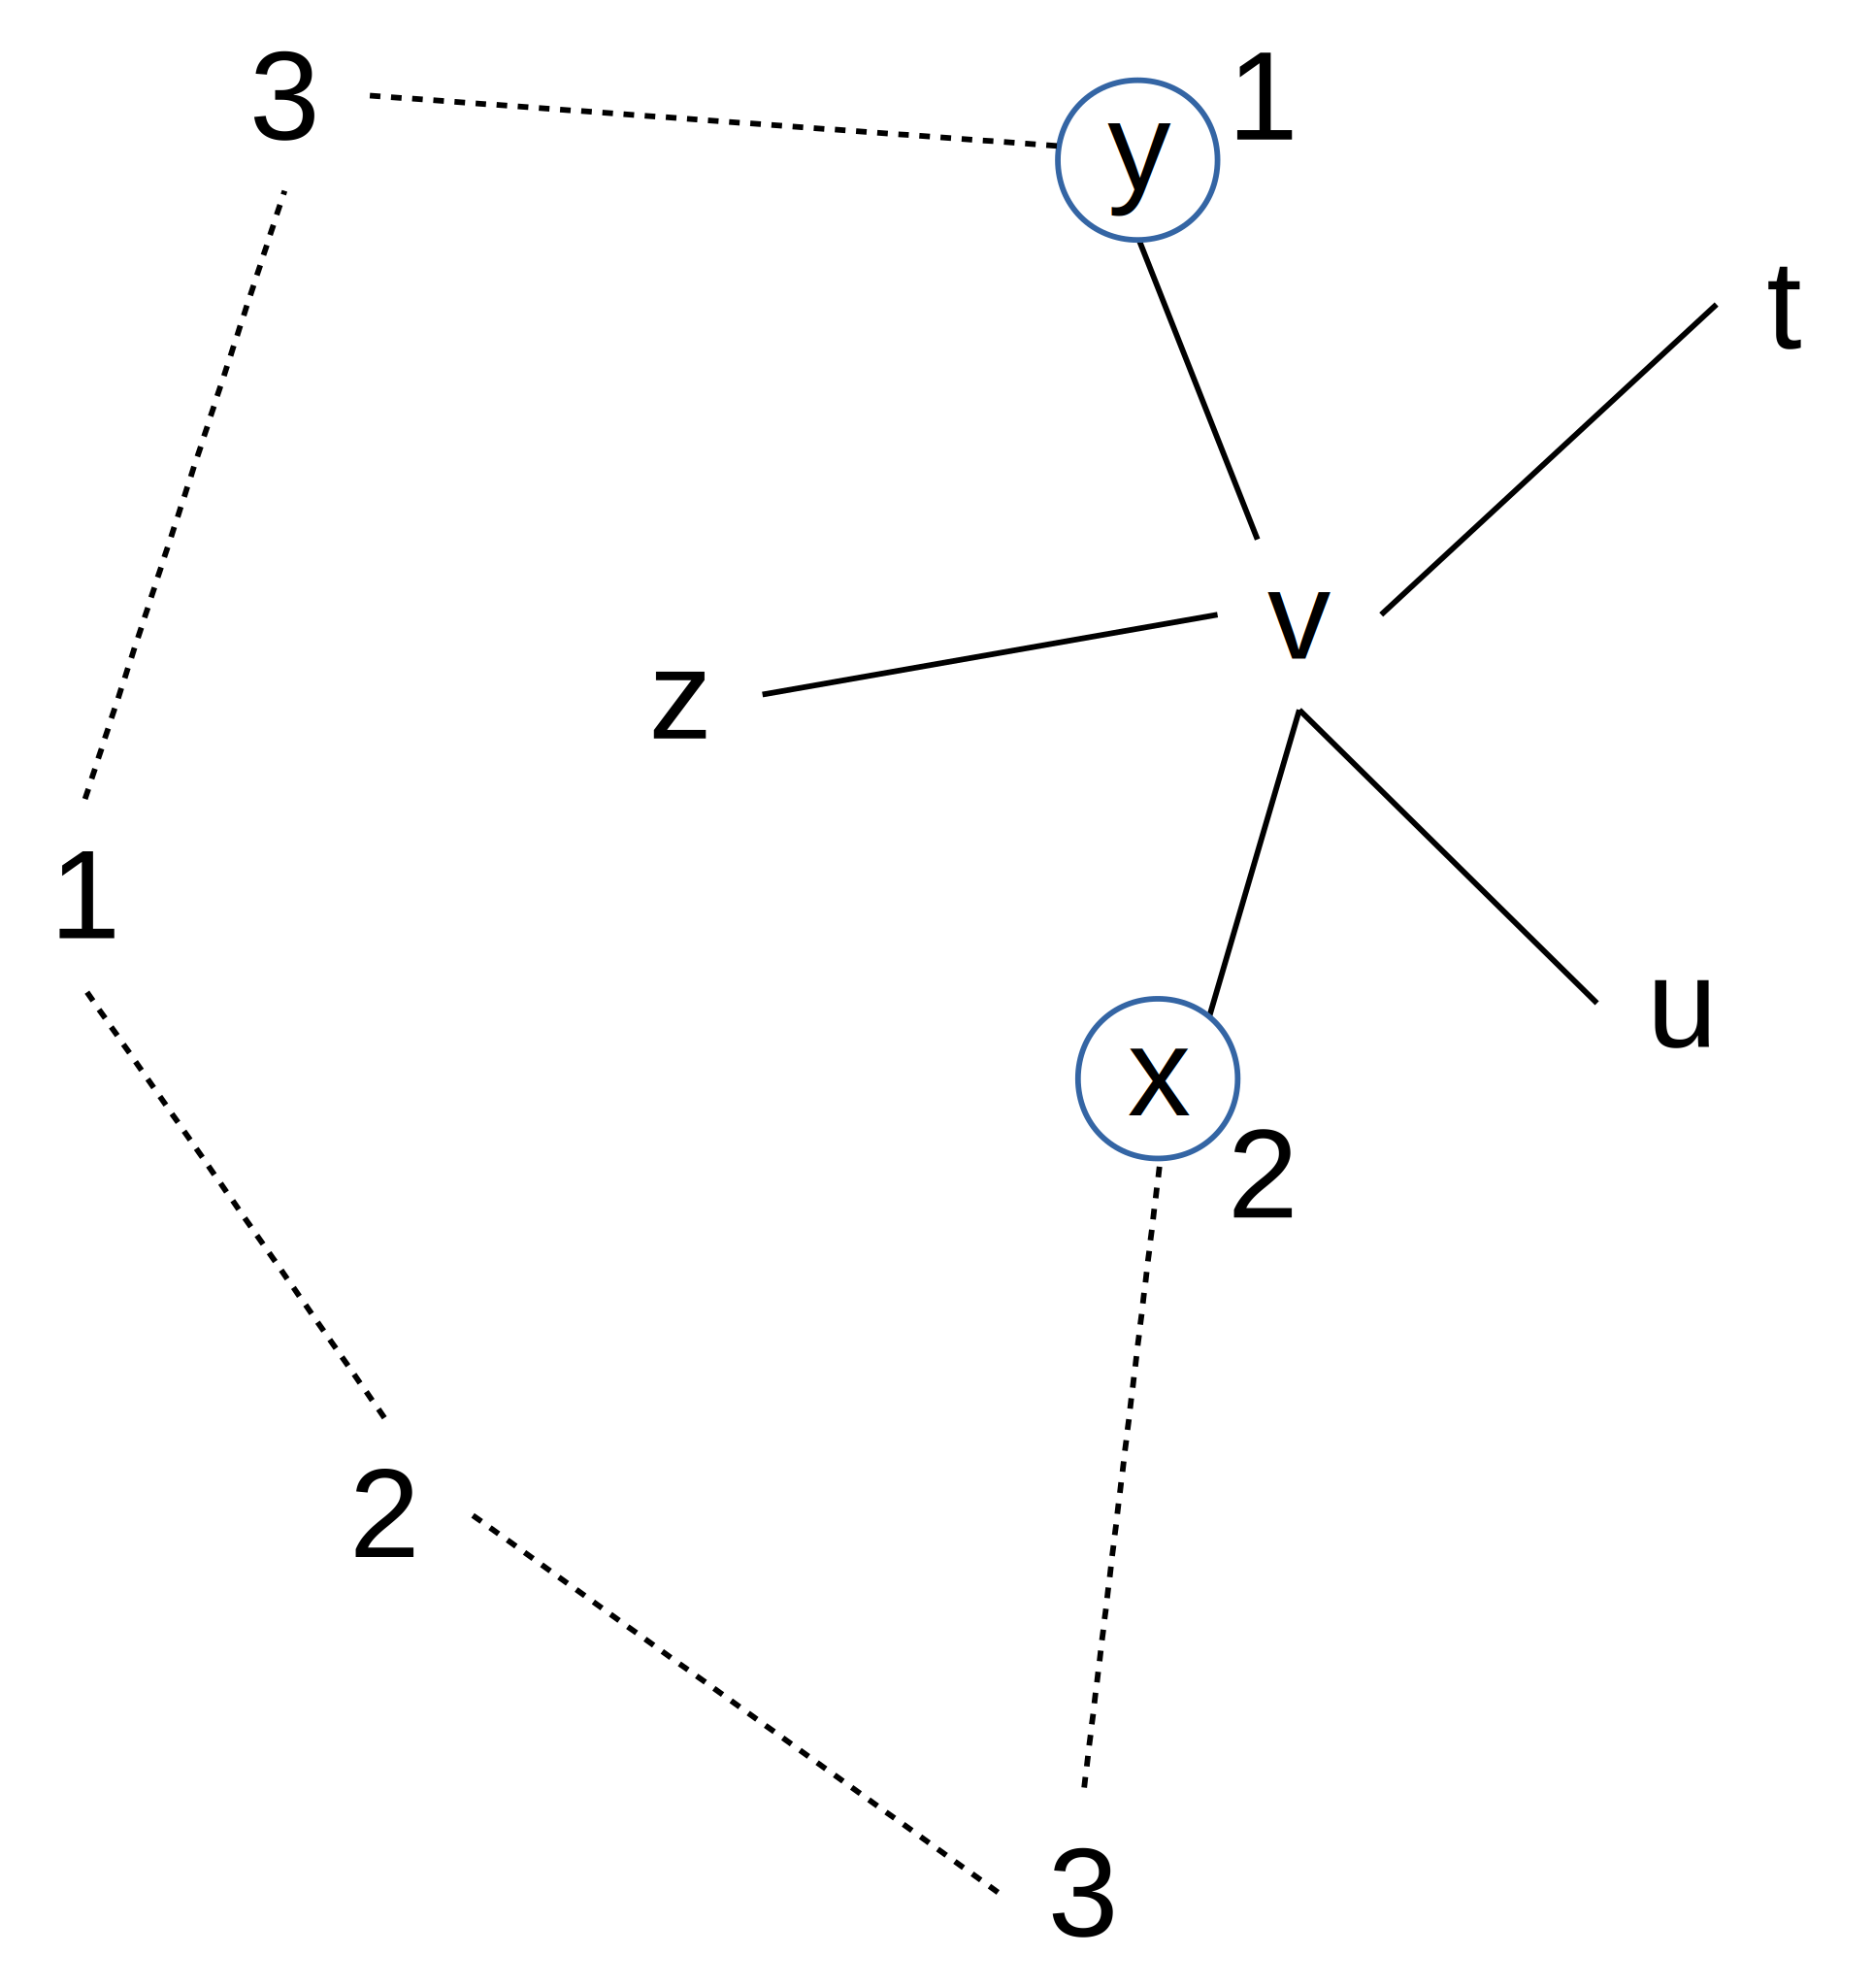
\includegraphics[scale=0.5]{lectures/161125/pix/2.pdf}
                        \begin{itemize}
                            \item betrachte 5-Färbung $\mathcal{C} \colon V(G \setminus \{v\}) \mapsto \{1, \dots, 5\}$, die es nach Rekursion gibt
                            \item betrache $x,y \in V_{xy}$ und sei $V_{xy} \subset V(G)$ die Menge der Knoten mit $\mathcal{C}(x)$- oder $\mathcal{C}(y)$-Färbung
                                \begin{enumerate}
                                    \item es gibt \underline{keinen} Weg von $x \rightsquigarrow y$, der nur Knoten aus $V_{xy}$ nutzt
                                        \begin{itemize}
                                            \item Seien $V'_{xy}$ die $s \in V(G \setminus \{v\})$, die von $x$ nur via $V_{xy}$ erreicht werden
                                            \item Färbe um:
                                            \begin{math}
                                                \mathcal{C'}(s) =
                                                    \begin{cases}
                                                        \mathcal{C}(s) & s \not \in V'_{xy}\\
                                                        \mathcal{C}(y) & s \in V'_{xy}, ~ \mathcal{C}(s) = \mathcal{C}(x)\\
                                                        \mathcal{C}(x) & s \in V'_{xy}, ~ \mathcal{C}(s) = \mathcal{C}(y)
                                                    \end{cases}
                                            \end{math}\\\\
                                            ``Tausche Farben auf $V'_{xy}$'' $\Rightarrow \mathcal{C'}(x) = \mathcal{C'}(y) = \mathcal{C}(y)$
                                        \end{itemize}
                                    \item es gibt einen solchen Pfad $x \rightsquigarrow y$ mit allen Knoten in $V_{xy}$
                                    \includegraphics[scale=0.5]{lectures/161125/pix/3.pdf}
                                        \begin{itemize}
                                            \item $V_{zt}$: alle Knoten in $V(G \setminus \{v\})$, die $\mathcal{C}(t)$ oder $\mathcal{C}(z)$ gefärbt sind
                                            \item $V_{xy} \cap V_{zt} = \emptyset$!
                                            \item $V'_{zt}$ kann nur via eines $s \in P$ einen Knoten in $V_{zt} \setminus V'_{zt}$ erreichen
                                        \end{itemize}
                                        Damit lassen sich $z,t$ analog zu Fall (a) färben.
                                \end{enumerate}
                        \end{itemize}
                \end{enumerate}
        \end{description}
    \item[Theorem] Jeder planare Graph ist 4-färbbar
        \begin{description}
            \item[Proof] Es gibt eine Menge von 1936 4-färbbaren Karten, jede nicht Teil eines kleinsten Gegenbeispiels... (Appel, Haken, 1976).
            $\Rightarrow$ Es folgt, dass es kein kleinstes Gegenbeispiel gibt.
        \end{description}
\end{description}

\subsection{Zufallsgraphen}
Sei $G=(V,E)$ mit $V=\{1, \dots, n\}$ fixiert. Wir wollen nun Kanten zufällig auswählen auf dieser fixierten Kantenmenge $\{1, \dots, n\}$, um zufällige Graphen zu generieren. 
Die Menge dieser Zufallsgraphen nennen wir $\mathcal{G}$. \underline{Jede} Kante wird mit Wahrscheinlichkeit $p \in [0, \dots, 1]$ gewählt. 
Sei $G_0$ ein bestimmter Graph. Das Ereignis $\{G_0\}$ mit $G_0$ und m Kanten hat die Wahrscheinlichkeit $p^m \cdot (1-p)^{{n \over 2}-m}$. 
Wahrscheinlichkeitsmaß auf 
$\mathcal{G} ~ \forall e \in [v]^2$\\
$\Omega_e=\{0_e, 1_e\}$\\
$\mathbb{P}(\{1_e\})=p$\\
$\mathbb{P}(\{0_e\})=1-p$\\
$\Omega_\mathcal{G} = \prod\limits_{e \in [v]^2} \Omega_e$

\begin{description}
    \item[Beispiele] Fixiere Graph $H$, $V(H) = V(G)$, ist $H \leqslant G$? \\
        Mit $p^l$, $|E(H)| = l$, $|V(H)| = k$, aber falls $H$ induzierter Teilgraph von $G$ sein soll? \\
         - Nur $p^l (1-p)^{\binom{k}{2} - l}$. \\
        Und was ist mit Subgraph-Isomorphismus?
        \includegraphics[scale=0.5]{lectures/161125/pix/4.pdf}
        \begin{itemize}
            \item Ereignismengen überlappen
            \item kompliziert
        \end{itemize}
\end{description}

\subsection{Eigenschaften fast aller Graphen}
Falls die Wahrscheinlichkeit, dass $P(G \in \mathcal{G}) \rightarrow 1$ für $n \rightarrow \infty$, dann geschieht $G$ fast sicher.
\begin{description}
    \item[Pro:] Gegeben jedes $H$ als Isomorphie-Klasse, $n \rightarrow \infty$ und $p \in ]0,1[ = (0,1)$, induzierte Kopie von $H$. 
    Dann haben fast alle $G$ in $\mathcal{G}(n,p)$ haben mindestens eine induzierte Kopie von $H$.
    \item[Prf:] Sei $H$ gegeben, $K=V(H)$. Sei $K \leqslant n$. $H$ ist (subgraph-) isomorph zu $G$ mit Wahrscheinlichkeit $r < 0$ ($G$ ist zufällig!). 
        Teile $G$ in $\lfloor {n \over k} \rfloor$ Teilgraphen, um genau so viele ``Versuche'' (für $r > 0$) zu haben. 
        $P(H \not \subseteq G$ induziert) $\leqslant (1-r)^{\lfloor {n \over k} \rfloor} \xrightarrow{n \rightarrow \infty} 0$
\end{description}


\newpage

\section{Vorlesung 25.11.2016}
\subsection{Färbung von Graphen}
\subsubsection{Vertexfärbung}
Zwei durch eine Kante verbundene Knoten haben unterschiedliche Farben.\\
Beispiel wäre eine Landkarte auf der mit so wenig wie möglich Farben die Länder ausgemalt werden, ohne zwei benachbarte Länder gleichfarbig zu haben. Hierbei entspricht jede Facette einen Knoten.\\
\includegraphics[width=0.4\textwidth]{lectures/161125/pix/Vertexfaerbung}
\begin{description}
    \item[Vertexfärbung] Eine Vertexfärbung eines Graphen $G=(V,E)$ ist eine Abbildung $\mathcal{C} \colon V \mapsto \mathcal{S}$, mit $\mathcal{S}=$ Menge der Farben. Es gilt, dass $\mathcal{C}(v) \neq \mathcal{C}(w)$, mit $w,v \in \mathcal{S}$, wenn $v$ und $w$ adjazent ($\{v,w\} \in E$) sind. Die Elemente von $\mathcal{S}$ heißen \emph{Farben}.
    \item[k-Färbung] Ein Graph $G$ ist $k$-färbbar, wenn es für eine Abbildung $\mathcal{C}$ eine Menge $\mathcal{S}=\{1,\dots,k\}$ gibt.
    \item[Chromatische Zahl] Eine chromatische Zahl $\chi(G)$ ist die kleinste natürliche Zahl $k$, sodass G $k$-färbbar ist. $\chi(G) \leqslant \Delta(G) + 1$, mit $\Delta(G) = $ maximaler Grad von $G$
        \begin{description}
            \item[Proof (greedy)] Färbe $v_i$ der Vertices $v_1 \dots v_n$ mit der kleinsten Farbe, die nicht von einem Nachbarn von $v_i$ benutzt wird. Da wir max. $\Delta(G)$ viele Nachbarn für $v_i$ haben, gibt es immer eine freie Farbe.
        \end{description}
        $\chi(G) \geqslant$ Größe der größten Clique
    \item[Lemma] Für jeden einfachen planaren Graphen $G$ ist der Durchschnittsgrad $d(G) < 6$
        \begin{description}
            \item[Proof] $d(G) = 2 \cdot {|E| \over |V|}$ mit $|V| \leqslant 3$, $|E| \leqslant 3  \cdot |V| - 6$, dann $d(G) \leqslant {2(3 \cdot |V|-6) \over |V|} = 6-{12 \over |V|}$
        \end{description}
    \item[Theorem] Jeder simple planare Graph $G$ hat $\chi(G) \leqslant 6$
        \begin{description}
            \item[Proof] Annahme: Jeder simple planare Graph mit $|V| = n$ ist $6$-färbbar.
            \begin{itemize}
                \item Sei $G$ hiermit ein simpler planarer Graph mit $|V| = n+1$
                \item Vom Lemma wissen wir, dass $w \in V$ mit $d(w) \leqslant 5$ existiert
                \item Sei $G' = G \setminus \{w\}$. Via Induktionshypothese ist $G'$ 6-färbbar. Das tun wir dann.
                \item Färbe $w$ mit der (min.) freien Farbe, um $G$ zu färben
            \end{itemize}
        \end{description}
    \item[Theorem] Für jeden simplen planaren Graphen $G$ gilt, dass $\chi(G) \leqslant 5$
        \begin{description}
            \item[Proof] Sei $G=(V,E)$ planar
                \begin{enumerate}
                    \item Falls $|V| \leqslant 5 \rightarrow$ trivial
                    \item Für alle $v \in V(G)$ mit $deg(v) < 5$, färbe $v$ und arbeite mit $G \setminus \{v\}$
                    \item $G$ hat Vertex $v$ mit $deg(v) = 5$
                        \includegraphics[scale=0.5]{lectures/161125/pix/2.pdf}
                        \begin{itemize}
                            \item betrachte 5-Färbung $\mathcal{C} \colon V(G \setminus \{v\}) \mapsto \{1, \dots, 5\}$, die es nach Rekursion gibt
                            \item betrache $x,y \in V_{xy}$ und sei $V_{xy} \subset V(G)$ die Menge der Knoten mit $\mathcal{C}(x)$- oder $\mathcal{C}(y)$-Färbung
                                \begin{enumerate}
                                    \item es gibt \underline{keinen} Weg von $x \rightsquigarrow y$, der nur Knoten aus $V_{xy}$ nutzt
                                        \begin{itemize}
                                            \item Seien $V'_{xy}$ die $s \in V(G \setminus \{v\})$, die von $x$ nur via $V_{xy}$ erreicht werden
                                            \item Färbe um:
                                            \begin{math}
                                                \mathcal{C'}(s) =
                                                    \begin{cases}
                                                        \mathcal{C}(s) & s \not \in V'_{xy}\\
                                                        \mathcal{C}(y) & s \in V'_{xy}, ~ \mathcal{C}(s) = \mathcal{C}(x)\\
                                                        \mathcal{C}(x) & s \in V'_{xy}, ~ \mathcal{C}(s) = \mathcal{C}(y)
                                                    \end{cases}
                                            \end{math}\\\\
                                            ``Tausche Farben auf $V'_{xy}$'' $\Rightarrow \mathcal{C'}(x) = \mathcal{C'}(y) = \mathcal{C}(y)$
                                        \end{itemize}
                                    \item es gibt einen solchen Pfad $x \rightsquigarrow y$ mit allen Knoten in $V_{xy}$
                                    \includegraphics[scale=0.5]{lectures/161125/pix/3.pdf}
                                        \begin{itemize}
                                            \item $V_{zt}$: alle Knoten in $V(G \setminus \{v\})$, die $\mathcal{C}(t)$ oder $\mathcal{C}(z)$ gefärbt sind
                                            \item $V_{xy} \cap V_{zt} = \emptyset$!
                                            \item $V'_{zt}$ kann nur via eines $s \in P$ einen Knoten in $V_{zt} \setminus V'_{zt}$ erreichen
                                        \end{itemize}
                                        Damit lassen sich $z,t$ analog zu Fall (a) färben.
                                \end{enumerate}
                        \end{itemize}
                \end{enumerate}
        \end{description}
    \item[Theorem] Jeder planare Graph ist 4-färbbar
        \begin{description}
            \item[Proof] Es gibt eine Menge von 1936 4-färbbaren Karten, jede nicht Teil eines kleinsten Gegenbeispiels... (Appel, Haken, 1976).
            $\Rightarrow$ Es folgt, dass es kein kleinstes Gegenbeispiel gibt.
        \end{description}
\end{description}

\subsection{Zufallsgraphen}
Sei $G=(V,E)$ mit $V=\{1, \dots, n\}$ fixiert. Wir wollen nun Kanten zufällig auswählen auf dieser fixierten Kantenmenge $\{1, \dots, n\}$, um zufällige Graphen zu generieren. 
Die Menge dieser Zufallsgraphen nennen wir $\mathcal{G}$. \underline{Jede} Kante wird mit Wahrscheinlichkeit $p \in [0, \dots, 1]$ gewählt. 
Sei $G_0$ ein bestimmter Graph. Das Ereignis $\{G_0\}$ mit $G_0$ und m Kanten hat die Wahrscheinlichkeit $p^m \cdot (1-p)^{{n \over 2}-m}$. 
Wahrscheinlichkeitsmaß auf 
$\mathcal{G} ~ \forall e \in [v]^2$\\
$\Omega_e=\{0_e, 1_e\}$\\
$\mathbb{P}(\{1_e\})=p$\\
$\mathbb{P}(\{0_e\})=1-p$\\
$\Omega_\mathcal{G} = \prod\limits_{e \in [v]^2} \Omega_e$

\begin{description}
    \item[Beispiele] Fixiere Graph $H$, $V(H) = V(G)$, ist $H \leqslant G$? \\
        Mit $p^l$, $|E(H)| = l$, $|V(H)| = k$, aber falls $H$ induzierter Teilgraph von $G$ sein soll? \\
         - Nur $p^l (1-p)^{\binom{k}{2} - l}$. \\
        Und was ist mit Subgraph-Isomorphismus?
        \includegraphics[scale=0.5]{lectures/161125/pix/4.pdf}
        \begin{itemize}
            \item Ereignismengen überlappen
            \item kompliziert
        \end{itemize}
\end{description}

\subsection{Eigenschaften fast aller Graphen}
Falls die Wahrscheinlichkeit, dass $P(G \in \mathcal{G}) \rightarrow 1$ für $n \rightarrow \infty$, dann geschieht $G$ fast sicher.
\begin{description}
    \item[Pro:] Gegeben jedes $H$ als Isomorphie-Klasse, $n \rightarrow \infty$ und $p \in ]0,1[ = (0,1)$, induzierte Kopie von $H$. 
    Dann haben fast alle $G$ in $\mathcal{G}(n,p)$ haben mindestens eine induzierte Kopie von $H$.
    \item[Prf:] Sei $H$ gegeben, $K=V(H)$. Sei $K \leqslant n$. $H$ ist (subgraph-) isomorph zu $G$ mit Wahrscheinlichkeit $r < 0$ ($G$ ist zufällig!). 
        Teile $G$ in $\lfloor {n \over k} \rfloor$ Teilgraphen, um genau so viele ``Versuche'' (für $r > 0$) zu haben. 
        $P(H \not \subseteq G$ induziert) $\leqslant (1-r)^{\lfloor {n \over k} \rfloor} \xrightarrow{n \rightarrow \infty} 0$
\end{description}


\end{document}